% input: [mainthesis.tex]
%This template was prepared by Dorothea F. Brosius of the 
%Institute for Electronics and Applied Physics, University of Maryland, College Park, MD
%The template was last updated in March 2013
%Thesis Main Page used with thesis.sty based on the
%University of Maryland Electronic Thesis and Dissertation (ETD) Style Guide

\documentclass[12pt]{thesis}  %12pt is larger than 11pt
%\usepackage[pctex32]{graphics}
\usepackage{titlesec}
   \titleformat{\chapter}
      {\normalfont\large}{Chapter \thechapter:}{1em}{}

\usepackage{longtable}
\usepackage{graphicx}
\usepackage[nocompress]{cite}
\usepackage{notoccite}
%\usepackage{lscape}
\usepackage{indentfirst}
%\usepackage{latexsym}
\usepackage{multirow}
\usepackage{bigstrut}
%\usepackage{tabls}
\usepackage{wrapfig}
\usepackage{slashbox}
\usepackage{supertabular}
%\usepackage{subeqn}
\usepackage{subfigure}
\usepackage{amsmath}
\usepackage{amssymb}
\usepackage{xspace}
\usepackage{setspace}
\usepackage[pagebackref=true,breaklinks=true,linktocpage=true,pdfstartview=FitH,plainpages=false,pdfpagelabels]{hyperref}
\usepackage{array}
\usepackage{afterpage}
\usepackage{pdflscape}

%%%%%%%%%%%%% ptdr definitions %%%%%%%%%%%%%%%%%%%%%
\usepackage{ptdr-definitions}
%%%%%%%%%%%%% Symbols %%%%%%%%%%%%%%%%%%%
% input: [symbols.tex]
%math
%\newcommand\triplet[3]{\left(\genfrac{}{}{0pt}{0}{#1}{\genfrac{}{}{0pt}{0}{#2}{#3}}\right)}
\newcommand\triplet[4][c]{\left(%
        \begin{array}{@{}#1@{}}#2\\#3\\#4%
\end{array}%
\right)%
}
\newcommand\doublet[3][c]{\left(%
        \begin{array}{@{}#1@{}}#2\\#3%
\end{array}%
\right)%
}

\newcommand{\neghphantom}[1]{\settowidth{\dimen0}{#1}\hspace*{-\dimen0}}

\newcommand{\tauh}{\ensuremath{\tau_{\text{h}}}\xspace}
\newcommand{\Pe}{\ensuremath{\cmsSymbolFace{e}}\xspace}
\newcommand{\Pep}{\ensuremath{\cmsSymbolFace{e}^{+}}\xspace}
\newcommand{\Pem}{\ensuremath{\cmsSymbolFace{e}^{-}}\xspace}
\newcommand{\Pp}{\ensuremath{\cmsSymbolFace{p}}\xspace}
\newcommand{\mutau}{\ensuremath{\mu\tauh}\xspace}
\newcommand{\etau}{\ensuremath{\Pe\tauh}\xspace}
%\newcommand{\etau}{\ensuremath{e\tauh}\xspace}
\newcommand{\emu}{\ensuremath{\Pe\mu}\xspace}
\newcommand{\ltau}{\ensuremath{\ell\tauh}\xspace}
\newcommand{\pbwo}{\ensuremath{\text{PbWO}_{4}}\xspace}
\newcommand{\MLQ}{\ensuremath{M_{\text{LQ}}}\xspace}
\newcommand{\Mstop}{\ensuremath{M_{\sTop}}\xspace}

%superfield symbols
\providecommand{\PU}{\ensuremath{\cmsSymbolFace{U}}\xspace}
\providecommand{\PD}{\ensuremath{\cmsSymbolFace{D}}\xspace}
\providecommand{\PQ}{\ensuremath{\cmsSymbolFace{Q}}\xspace}
\providecommand{\PE}{\ensuremath{\cmsSymbolFace{E}}\xspace}
\providecommand{\PL}{\ensuremath{\cmsSymbolFace{L}}\xspace}

%units
\newcommand{\muA}{\ensuremath{\,\mu\text{A}}\xspace}
\newcommand{\degC}{\ensuremath{\,\de\text{C}}\xspace}

\def\BAL{\ensuremath{B_{\met}}}
\def\MET{\ensuremath{{E\!\!\!/}_{\mathrm{T}}}}
\def\METV{\ensuremath{\vec{E\!\!\!/}_{\mathrm{T}}}}
\def\QT{\ensuremath{{q}_{\mathrm{T}}}}
\def\QTV{\ensuremath{\vec{q}_{\mathrm{T}}}}
\def\PT{\ensuremath{{p}_{\mathrm{T}}}}
\def\ET{\ensuremath{{E}_{\mathrm{T}}}}
\def\HT{\ensuremath{{H}_{\mathrm{T}}}}


\def\eslash{\ensuremath{{\hbox{$E$\kern-0.6em\lower-.05ex\hbox{/}\kern0.10em}}}}
\def\vecmet{\mbox{$\vec{\eslash}_\text{T}$}\xspace} %missing ET vector
\def\vecet{\mbox{$\vec{E}_\text{T}$}\xspace} % ET vector
\def\vecpt{\mbox{$\vec{p}_\text{T}$}\xspace} % PT vector
\def\met{\mbox{$\eslash_\text{T}$}\xspace} %missing ET, no space
\def\mex{\mbox{$\eslash_x$}\xspace} %missing Ex
\def\mey{\mbox{$\eslash_y$}\xspace} %missing Ey
\def\mepar{\mbox{$\eslash_\parallel$}\xspace}
\def\meperp{\mbox{$\eslash_\perp$}\xspace}
\def\metvec{\mbox{$\vec{\met}$}\xspace}
\def\metvecrec{\mbox{$\vec{\met}^{\rm rec}$}\xspace}
\def\metvecgen{\mbox{$\vec{\met}^{\rm gen}$}\xspace}
\def\metgen{\mbox{$\met^{\rm gen}$}\xspace}
\def\metparl{\mbox{$\mepar^{\rm rec}$}\xspace}
\def\metperp{\mbox{$\meperp^{\rm rec}$}\xspace}
\def\deltamet{\mbox{$\Delta\met$}\xspace}
\def\pthat{\mbox{$\hat{p}_T$}\xspace}
\def\hslash{{\hbox{$H$\kern-0.8em\lower-.05ex\hbox{/}\kern0.10em}}}
\def\MHT{\mbox{$\hslash_\text{T}$}\xspace}
\def\mht{\mbox{$\hslash_\text{T}$}\xspace}
\def\sumet{\mbox{$\sum E_\text{T}$}\xspace}
\def\scalht{\mbox{$H_\text{T}$}\xspace}
\def\etmiss{\eslash_T}
\def\qt{\ensuremath{{q}_{\mathrm{T}}}}
\def\bigeslash{{\hbox{$E$\kern-0.38em\lower-.05ex\hbox{/}\kern0.10em}}}  
\def\bigmet{\mbox{$\bigeslash_T$}\xspace} 
\def\bighslash{{\hbox{$H$\kern-0.6em\lower-.05ex\hbox{/}\kern0.10em}}}  
\def\bigmht{\mbox{$\bighslash_T$}\xspace} 
\def\vecut{\mbox{$\vec{u}_T$}\xspace}

\def\Lum{\mbox{$\mathcal{L}$}\xspace}
\def\Acc{\mbox{$\mathcal{A}$}\xspace}
\def\eps{\mbox{$\epsilon$}\xspace}

%%%%
%%%% Additional definitions by GHM
%%%%
\def\ERROR#1#2{ \ensuremath{ \pm #1\, (\textrm{#2}) }  }
\def\RESA#1#2#3{ \ensuremath{ #1 \ERROR{#2}{#3} } }
\def\RESB#1#2#3#4#5{ \ensuremath{ \RESA{#1}{#2}{#3} \ERROR{#4}{#5} } }
\def\RESC#1#2#3#4#5#6#7{ \ensuremath{ \RESB{#1}{#2}{#3}{#4}{#5} \ERROR{#6}{#7} } }
\def\RESD#1#2{ \ensuremath{ #1 \pm #2 } }
\def\EFF#1#2{ \ensuremath{ ( \RESA{#1}{#2}{stat.} )\% } }
\def\EFFA#1#2{ \ensuremath{ ( {#1} \pm {#2} )\% } }
\def\EFFB#1#2#3{ \ensuremath{ ( \RESA{#1}{#2}{stat.} \ERROR{#3}{syst.} )\% } }
\def\SIGBR#1#2{  \ensuremath{ \sigma \left( \pp \to #1 X \right) \times {\cal{B}} \left( #1 \to #2 \right) } }
\def\SIGBRSHORT#1{\ensuremath{ [\, \sigma\times{\cal{B}}\, ](#1) }}
\def\SIGSHORT#1{\ensuremath{ \sigma(#1) }}
\def\RESE#1#2#3#4{ \ensuremath{ \RESC{#1}{#2}{stat.}{#3}{syst.}{#4}{lumi.} }}
\def\RESF#1#2#3{ \ensuremath{ \RESB{#1}{#2}{stat.}{#3}{syst.} }}
\def\RATWZ#1#2{ \ensuremath{ {
 \frac{ \sigma(\pp\rightarrow \PW X)\times {\cal{B}}(\PW\rightarrow #1)  }
      { \sigma(\pp\rightarrow \PZ X)\times {\cal{B}}(\PZ\rightarrow #2)  }   }  } }
\def\RESRATWZ#1#2#3#4#5{ \ensuremath{ \RATWZ{#1}{#2} &=& 
                                   #3 \ERROR{#4}{stat.} \ERROR{#5}{syst.} } }
\def\RATWW#1#2{ \ensuremath{ {
 \frac{ \sigma(\pp\rightarrow \PWp X)\times {\cal{B}}(\PWp\rightarrow #1)  }
      { \sigma(\pp\rightarrow \PWm X)\times {\cal{B}}(\PWm\rightarrow #2)  }   }  } }
\def\RESRATWW#1#2#3#4#5{ \ensuremath{ \RATWW{#1}{#2} &=& 
                                   #3 \ERROR{#4}{stat.} \ERROR{#5}{syst.} } }
\def\THEORYRATIO#1#2{\ensuremath{ \RESD{#1}{#2} }}
\def\EPS#1{ \ensuremath{ \epsilon_{\textrm{#1}} } }
\def\EPSTNPALL#1{ \ensuremath{ \EPS{TNP-WP{#1}-ALL}  }  }
\def\EPSTNPREC{ \ensuremath{ \EPS{TNP-REC} }  }
\def\EPSTNPTRG{ \ensuremath{ \EPS{TNP-TRG} }  }
\def\EPSTNPWP#1{ \ensuremath{ \EPS{TNP-WP{#1} } }  }
\def\EPSTNPTRGWP#1{ \ensuremath{ \EPS{TNP-TRG{#1}} }  } 
\def\XVL#1#2{ \ensuremath{#1_{#2}} }
\def\NSIG#1{ \ensuremath{\XVL{N}{#1} } }
\def\EPSB#1{ \ensuremath{\XVL{\varepsilon}{#1} } }
\def\RHO#1{ \ensuremath{\XVL{\rho}{#1} } }
\def\AGEN#1{ \ensuremath{\XVL{A}{#1} } }
\def\APRIM#1{ \ensuremath{\XVL{ {F} }{#1} } }
\def\RPM{\ensuremath{R_{\scriptscriptstyle{+/-}} }}
\def\RWZ{\ensuremath{R_{\scriptscriptstyle{\PW/\PZ}} }}


%%%%%%%%%%%%%%%%%%%%%%%%%%%%%%%%%%%%%%%%%%%%%%%%%%%%%%%%%%%%%%%%%%%%%%
\newcommand{\THELUMI} {\ensuremath{{2.88\pm 0.32}~\mathrm{pb}^{-1}}}%


%%%%%%%%%%%%%%%  Additional definitions %%%%%%%%%%%%%%%%%%%%%%%%
%\renewcommand{\PJgy}{\ensuremath{\mathrm{J}\hspace{-.08em}/\hspace{-.14em}\psi}}
\renewcommand{\ttbar}{\ensuremath{\mathrm{t}\overline{\mathrm{t}}}\xspace}
\newcommand{\singletop}{\ensuremath{\mathrm{single-t}}}
\newcommand{\pp}{\ensuremath{{\Pp\Pp}}\xspace}%
\newcommand{\PZ}{\ensuremath{{\mathrm{Z}}}\xspace}%
\newcommand{\PV}{\ensuremath{{\mathrm{V}}}\xspace}%
\newcommand{\rts}{\ensuremath{\sqrt{s}}\xspace}%
\newcommand{\ra}{\ensuremath{\rightarrow}}%


%\def\Zll{\ensuremath{Z \to \ell\ell}\xspace}
%\def\Wmn{\ensuremath{W \to \mu\nu}\xspace}
%\def\Wen{\ensuremath{W \to e\nu}\xspace}
%\def\Wln{\ensuremath{W \to \ell\nu}\xspace}

\newcommand{\MN}{\ensuremath{\Pgm\nu}}%
\newcommand{\MpN}{\ensuremath{\Pgmp\nu}}%
\newcommand{\MmN}{\ensuremath{\Pgmm\overline{\nu}}}%
\newcommand{\EN}{\ensuremath{\Pe\nu}}%
\newcommand{\EpN}{\ensuremath{\Pep\nu}}%
\newcommand{\EmN}{\ensuremath{\Pem\overline{\nu}}}%
\newcommand{\TN}{\ensuremath{\Pgt\nu}}%
\newcommand{\TpN}{\ensuremath{\Pgt^+\nu}}%
\newcommand{\TmN}{\ensuremath{\Pgt^-\overline{\nu}}}%
\newcommand{\LN}{\ensuremath{\ell\nu}}%
\newcommand{\LpN}{\ensuremath{\ell^+\nu}}%
\newcommand{\LmN}{\ensuremath{\ell^-\overline{\nu}}}%

\newcommand{\EpEm}{\ensuremath{\Pep\Pem}}%
\newcommand{\MpMm}{\ensuremath{\Pgmm\Pgmp}}%
\newcommand{\TpTm}{\ensuremath{\tau^+\tau^-}}%
\newcommand{\LpLm}{\ensuremath{\ell^+\ell^-}}%
%\newcommand{\EE}{\ensuremath{\Pe\Pe}}%
%\newcommand{\MM}{\ensuremath{\Pgm\Pgm}}%
%\newcommand{\TT}{\ensuremath{\tau\tau}}%
%\newcommand{\LL}{\ensuremath{\ell\ell}}%
\newcommand{\MW}{\ensuremath{{m}_\PW}}%
\newcommand{\MZ}{\ensuremath{{m}_\PZ}}%
\newcommand{\MT}{\ensuremath{{M}_{\text{T}}}\xspace}%
\newcommand{\MLL}{\ensuremath{{M}_{\LpLm}}}%

\newcommand{\Wmn}{\ensuremath{\PW \ra \MN}}%
\newcommand{\Wpmn}{\ensuremath{\PWp \ra \MpN}}%
\newcommand{\Wmmn}{\ensuremath{\PWm \ra \MmN}}%
%\newcommand{\Zmm}{\ensuremath{\PZ \ra \MpMm}\xspace}%
\newcommand{\Zmm}{\ensuremath{\Z \ra \mu\mu}\xspace}%
\newcommand{\Znn}{\ensuremath{\PZ \ra \nu\nu}}%
\newcommand{\ZLL}{\ensuremath{\PZ \ra \ell\ell}\xspace}%
\newcommand{\ppWmn}{\pp \ra \PW + X \ra \MN + X}%
\newcommand{\ppWpmn}{\pp \ra \PWp + X \ra \MpN + X}%
\newcommand{\ppWmmn}{\pp \ra \PWm + X \ra \MmN + X}%
\newcommand{\ppZmm}{\pp \ra \PZ + X \ra \MpMm + X}%

\newcommand{\Wen}{\ensuremath{\PW \ra \EN}}%
\newcommand{\Wpen}{\ensuremath{\PWp \ra \EpN}}%
\newcommand{\Wmen}{\ensuremath{\PWm \ra \EmN}}%
\newcommand{\Zee}{\ensuremath{\PZ \ra \EpEm}}%
\newcommand{\ppWen}{\pp \ra \PW + X \ra \EN + X}%
\newcommand{\ppWpen}{\pp \ra \PWp + X \ra \EpN  + X}%
\newcommand{\ppWmen}{\pp \ra \PWm + X \ra \EmN + X}%
\newcommand{\ppZee}{\pp \ra \PZ + X \ra \EpEm + X}%

\newcommand{\Wtn}{\ensuremath{\PW \ra \TN}}%
\newcommand{\Wptn}{\ensuremath{\PWp \ra \TpN}}%
\newcommand{\Wmtn}{\ensuremath{\PWm \ra \TmN}}%
\newcommand{\Ztt}{\ensuremath{\PZ \ra \TpTm}\xspace}%
\newcommand{\Zttll}{\ensuremath{\PZ \ra \TpTm/\LpLm}\xspace}%

%\newcommand{\Wln}{\ensuremath{\PW \ra \LN}}%
\newcommand{\Wln}{\ensuremath{\W \rightarrow \ell\nu}\xspace}%
\newcommand{\Wpln}{\ensuremath{\PWp \ra \LpN}}%
\newcommand{\Wmln}{\ensuremath{\PWm \ra \LmN}}%
\newcommand{\Zll}{\ensuremath{\PZ \ra \LpLm}\xspace}%
\newcommand{\ppZll}{\pp \ra \PZ + X \ra \LpLm + X}%
\newcommand{\ppWln}{\pp \ra \PW + X \ra \LN + X}%
\newcommand{\ppWpln}{\pp \ra \PWp + X \ra \LpN  + X}%
\newcommand{\ppWmln}{\pp \ra \PWm + X \ra \LmN + X}%

\newcommand{\gammaZ}{\ensuremath{\PZ/\gamma^{*}}}
\newcommand{\gammaZmm}{\mbox{$ \gammaZ\rightarrow \MpMm$}}
\newcommand{\gammaZee}{\mbox{$ \gammaZ\rightarrow \EpEm$}}
\newcommand{\gammaZtt}{\mbox{$ \gammaZ\rightarrow \TpTm$}}
\newcommand{\gammaZll}{\mbox{$ \gammaZ\rightarrow \LpLm$}}

\def\ZZ{\ensuremath{\PZ\PZ}\xspace}
\def\WZ{\ensuremath{\PW\PZ}\xspace}
\def\WW{\ensuremath{\PW\PW}\xspace}
\def\NN{\ensuremath{\nu \nu }\xspace }
\def\ZZllnn{\ensuremath{\ZZ \to \ell\ell\nu\nu}\xspace}
\def\ZZllll{\ensuremath{\ZZ \to 4\ell}\xspace}
\def\ZZeenn{\ensuremath{\ZZ \to \Pe\Pe\nu\nu}\xspace}
\def\ZZmmnn{\ensuremath{\ZZ \to \Pgm\Pgm\nu\nu}\xspace}
\def\WWllnn{\ensuremath{\WW \to \LN\LN}\xspace}
\def\WWeenn{\ensuremath{\WW \to \Pe\nu\Pe\nu}\xspace}
\def\WWmmnn{\ensuremath{\WW \to \Pgm\nu\Pgm\nu}\xspace}
\def\WWemnn{\ensuremath{\WW \to \Pe\nu\Pgm\nu}\xspace}
\def\WZllln{\ensuremath{\WZ \to \LN\ell\ell}\xspace}
\def\Zllj{\ensuremath{\ZLL + X}\xspace}
\def\WJ{\ensuremath{\PW+{\mathrm{jets}} }\xspace}
\def\WJo{\ensuremath{\PW+{\mathrm{1-jet}} }\xspace}
\def\ZJ{\ensuremath{\PZ+{\mathrm{jets}} }\xspace}
\def\VJ{\ensuremath{\PV+{\mathrm{jets}} }\xspace}
\def\GJ{\ensuremath{\gamma+{\mathrm{jets}} }\xspace}
\def\GamJ{\ensuremath{\gamma+{\mathrm{jets}} }\xspace}
\def\GZJ{\ensuremath{\gamma/\PZ+{\mathrm{jets}} }\xspace}
\def\VGam{\ensuremath{\PV+\Pgg }\xspace}
\def\WGam{\ensuremath{\PW+\Pgg }\xspace}
\def\ZGam{\ensuremath{\PZ+\Pgg }\xspace}


\newcommand{\mz}{\mbox{$m_{\PZ}$}}
\newcommand{\hta}{\mbox{$\eta$}}
\newcommand{\fh}{\mbox{$\phi$}}
\newcommand{\etot}{\mbox{$\epsilon_{tot}$}}
\newcommand{\eclustering}{\mbox{$ \epsilon_{clustering}$}}
\newcommand{\etracking}{\mbox{$ \epsilon_{tracking}$}}
\newcommand{\egsfele}{\mbox{$ \epsilon_{gsfele}$}}
\newcommand{\epreselection}{\mbox{$ \epsilon_{preselection}$}}
\newcommand{\eisolation}{\mbox{$ \epsilon_{isolation}$}}
\newcommand{\eclassification}{\mbox{$ \epsilon_{classification}$}}
\newcommand{\eelID}{\mbox{$ \epsilon_{elID}$}}
\newcommand{\etrigger}{\mbox{$ \epsilon_{trigger}$}}

\newcommand{\DE}{$\Delta\eta_{in}$}
\newcommand{\DP}{$\Delta\phi_{in}$}
\newcommand{\SEE}{$\sigma_{\eta\eta}$~}
\newcommand{\SEP}{$\sigma_{\eta\phi}$}
\newcommand{\SPP}{$\sigma_{\phi\phi}$}
\newcommand{\SXY}{$\sigma_{XY}$}
\newcommand{\pth}{\hat{p}_{\perp}}
\newcommand{\Lint}{\ensuremath{{\cal L}_{\mathrm{int}}}}
\newcommand{\IECAL}    {I^{\textrm{rel}}_{\scriptscriptstyle{\textrm{ECAL}}}}%
\newcommand{\IHCAL}    {I^{\textrm{rel}}_{\scriptscriptstyle{\textrm{HCAL}}}}%
\newcommand{\ITRK}     {I^{\textrm{rel}}_{\scriptscriptstyle{\textrm{trk}}}}%
\newcommand{\IRelComb} {I^{\textrm{rel}}_{\scriptscriptstyle{\textrm{comb}}}}%
\newcommand{\Nev}    {N_{\mathrm{ev}}}
\newcommand{\Nsig}   {N_{\mathrm{sig}}}
\newcommand{\Nsel}   {N_{\mathrm{sel}}}
\newcommand{\Nbg}    {N_{\mathrm{bg}}}
\newcommand{\rhoeff} {\rho_{\mathrm{eff}}}
\newcommand{\etaSC}  {\eta_{\mathrm{SC}}}


\def\effmc{\ensuremath{\epsilon_{\mathrm{sim}}}\xspace}
\def\effdt{\ensuremath{\epsilon_{\mathrm{data}}}\xspace}
\def\PUMET{\ensuremath{{\MET}^{\mathrm{PU}}}}
\def\PUMETMIN{\ensuremath{{\MET}^{\mathrm{PU,min}}}}
\def\CORRMET{\ensuremath{{\MET}^{\mathrm{corr}}}}

\def\sieie{\ensuremath{\sigma_{i\eta i\eta}}}
\def\sipip{\ensuremath{\sigma_{i\phi i\phi}}}

\def\ST{\ensuremath{S_{\text{T}}}\xspace}

\def\MassTJ{\ensuremath{M(\tauh,\text{jet})}\xspace}
\def\MassLJ{\ensuremath{M(\ell,\text{jet})}\xspace}



\def\tauf{\ensuremath{\tau_{f}}\xspace}

%\def\symexamp{stone}{\stone}
%\def\symexamp{sttwo}{\sttwo}
\def\stone{\ensuremath{\tilde{\rm{t}}_1}}
\def\sttwo{\ensuremath{\tilde{\rm{t}}_2}}

%\def\effdt{\ensuremath{\varepsilon_{\rm data}}\xspace}
%\def\effmc{\ensuremath{\varepsilon_{\rm MC }}\xspace}

%
% results
%



% yields

% integrated luminosity
\newcommand{\thelumi}{\ensuremath{19.7~\fbinv}\xspace}

%acceptance, efficiencies



% fake rate numbers

\def\tfmc{\ensuremath{2.22 \pm 0.50 \%}\xspace}
\def\tfd{\ensuremath{2.44 \pm 0.53 \%}\xspace} 



% background Numbers
\def\ttbbkgElLMass{\ensuremath{ 11.0\pm1.48 \ \mathrm{(stat.)} }\xspace}
\def\dibbkgElLMass{\ensuremath{ 2.14\pm0.81 \ \mathrm{(stat.)} }\xspace}
\def\zttbkgElLMass{\ensuremath{ 0.31\pm0.09 \ \mathrm{(stat.)} }\xspace}

\def\ttbbkgElHMass{\ensuremath{ 6.89\pm1.12 \ \mathrm{(stat.)} }\xspace}
\def\dibbkgElHMass{\ensuremath{ 2.14\pm0.81 \ \mathrm{(stat.)} }\xspace}
\def\zttbkgElHMass{\ensuremath{ 0.17\pm0.07 \ \mathrm{(stat.)} }\xspace}


\def\ttbbkgMuLMass{\ensuremath{ 38.1\pm2.87 \ \mathrm{(stat.)} }\xspace}
\def\dibbkgMuLMass{\ensuremath{ 5.02\pm1.51 \ \mathrm{(stat.)} }\xspace}
\def\zttbkgMuLMass{\ensuremath{ 0.51\pm0.12 \ \mathrm{(stat.)} }\xspace}

\def\ttbbkgMuHMass{\ensuremath{ 27\pm2.42 \ \mathrm{(stat.)} }\xspace}
\def\dibbkgMuHMass{\ensuremath{ 5.02\pm1.51 \ \mathrm{(stat.)} }\xspace}
\def\zttbkgMuHMass{\ensuremath{ 0.41\pm0.11 \ \mathrm{(stat.)} }\xspace}

% uncertainty numbsers

\def\UncPUMax{\ensuremath{6 \%}\xspace}
\def\UncPU{\ensuremath{ 3 \% }\xspace}

\def\UncBTS{\ensuremath{ 3 \% }\xspace}
\def\UncBTB{\ensuremath{ 2 \% }\xspace}
\def\UncBSF{\ensuremath{ 4 \% }\xspace}
\def\UncLSF{\ensuremath{ 10 \% }\xspace}
\def\UncBT{\ensuremath{ 2\mbox{-}3 \% }\xspace}
\def\UncBTSEff{\ensuremath{ 1 \% }\xspace}
\def\UncBTBEff{\ensuremath{ 2 \% }\xspace}
\def\UncBSFSig{\ensuremath{ 2 \% }\xspace}
\def\UncBSFtt{\ensuremath{ 2 \% }\xspace}
\def\UncBSFsinglet{\ensuremath{ 1 \% }\xspace}
\def\UncBSFZtt{\ensuremath{ <1 \% }\xspace}
\def\UncBSFEWK{\ensuremath{ 1 \% }\xspace}
\def\UncLSFSig{\ensuremath{ 2 \% }\xspace}
\def\UncLSFtt{\ensuremath{ 2 \% }\xspace}
\def\UncLSFZtt{\ensuremath{ 7 \% }\xspace}
\def\UncLSFEWK{\ensuremath{ 6 \% }\xspace}
\def\UncLSFsinglet{\ensuremath{ 3 \% }\xspace}

\def\UncBMTS{\ensuremath{ 2 \% }\xspace}
\def\UncBMTB{\ensuremath{ 5 \%  }\xspace}
\def\UncBMT{\ensuremath{ 2\mbox{-}5 \% }\xspace}
\def\UncBMTSEff{\ensuremath{ 1\% }\xspace}
\def\UncBMTBEff{\ensuremath{ 2\mbox{-}12\% }\xspace}

\def\UncTTBNorm{\ensuremath{ 19\mbox{-}22\% }\xspace}
\def\UncZttNorm{\ensuremath{ 2 \%}\xspace}
\def\UncDibNorm{\ensuremath{ 5-14 \% }\xspace} %5,9,14 -> WZ,WW,ZZ
\def\UncSingleTopNorm{\ensuremath{ 14 \% }\xspace} %14 -> t data ; 4-6-9 MC (s,tW,t)

\def\UncFake{\ensuremath{ 16\mbox{-}24\% }\xspace}
\def\UncFakeSEff{\ensuremath{ 0\% }\xspace}
\def\UncFakeBEff{\ensuremath{ 22\% }\xspace}
%\def\UncFakeMu{\ensuremath{ \% }\xspace}

\def\UncElESEB{\ensuremath{ 1 \% }\xspace}
\def\UncElESEE{\ensuremath{ 2.5 \% }\xspace}


\def\UncMuES{\ensuremath{ 1 \% }\xspace}
\def\UncTauES{\ensuremath{ 3 \% }\xspace}
\def\UncTauER{\ensuremath{ 10 \% }\xspace}
\def\UncJES{\ensuremath{ \sim 4 \% }\xspace}
\def\UncJER{\ensuremath{ 5\mbox{-}10 \% }\xspace}

\def\UncLumi{\ensuremath{2.6 \% }\xspace}
\def\UncTrig{\ensuremath{ 2 \% }\xspace}

\def\UncElId{\ensuremath{ 2 \% }\xspace}
\def\UncElIdSEff{\ensuremath{ 2 \% }\xspace}
\def\UncElIdBEff{\ensuremath{ 2 \% }\xspace}

\def\UncMuId{\ensuremath{ 2 \% }\xspace}
\def\UncMuIdSEff{\ensuremath{ 2 \% }\xspace}
\def\UncMuIdBEff{\ensuremath{ 2 \% }\xspace}

\def\UncTauId{\ensuremath{ 6 \% }\xspace}
\def\UncTauIdSEff{\ensuremath{ 6 \% }\xspace}
\def\UncTauIdBEff{\ensuremath{ 6 \% }\xspace}

%\def\TotUncSig{\ensuremath{ 6.5 \% }\xspace}
\def\TotUncSig{\ensuremath{ 8.6-13.9 \% }\xspace}
\def\TotUncBkg{\ensuremath{ 23-32\%}\xspace}
\def\TotUncBkgFake{ \ensuremath{ 16\mbox{-}24\%}\xspace}
\def\TotUncBkgTtb{ \ensuremath{ 13\mbox{-}17\%}\xspace}


%% tau/jet ES ER
\def\UncJESBkg{\ensuremath{0-7\%}\xspace}
\def\UncJERBkg{\ensuremath{0-5\%}\xspace}
\def\UncTESBkg{\ensuremath{5-19\%}\xspace}
\def\UncTERBkg{\ensuremath{20 \%}\xspace}

\def\UncJESSig{\ensuremath{\sim 1\%}\xspace}
\def\UncJERSig{\ensuremath{\sim 1\%}\xspace}
\def\UncTESSig{\ensuremath{0-5\%}\xspace}
\def\UncTERSig{\ensuremath{1-9\%}\xspace}


\newcommand{\tbsp}{\rule{0pt}{18pt}} %used to get a vertical distance after \hline
\renewcommand{\baselinestretch}{2}
\setlength{\textwidth}{5.9in}
\setlength{\textheight}{9in}
\setlength{\topmargin}{-.50in}
%\setlength{\topmargin}{0in}    %use this setting if the printer makes the the top margin 1/2 inch instead of 1 inch
\setlength{\oddsidemargin}{.55in}
\setlength{\parindent}{.4in}
\pagestyle{empty}
\setcounter{tocdepth}{3}
\setcounter{secnumdepth}{3}

%adjust spacing between equations and text
\makeatletter
\g@addto@macro\normalsize{%
  \setlength\abovedisplayskip{0.1\baselineskip}
  \setlength\belowdisplayskip{0.1\baselineskip}
  \setlength\abovedisplayshortskip{0.1\baselineskip}
  \setlength\belowdisplayshortskip{0.1\baselineskip}
}
\makeatother

\begin{document}

% input: [Abstract.tex]
%Abstract Page 

\hbox{\ }

\renewcommand{\baselinestretch}{1}
\small \normalsize

\begin{center}
\large{{ABSTRACT}} 

\vspace{3em} 

\end{center}

\begin{singlespace}

\noindent
\begin{tabular}{@{}ll}
Title of dissertation:    & {\large  Search for Pair Production of}\\
                          & {\large  Third-Generation Scalar Leptoquarks} \\
                          & {\large  and R-Parity Violating Top Squarks} \\
                          & {\large  in Proton-Proton Collisions at $\sqrt{s} = 8\TeV$} \\
                          & \\
                          & {\large  Kevin Pedro, Doctor of Philosophy, 2014} \\
                          & \\
Dissertation directed by: & {\large  Professor Sarah C. Eno} \\
                          & {\large  Department of Physics } \\
\end{tabular}

\end{singlespace}

\vspace{3em}

\renewcommand{\baselinestretch}{2}
\large \normalsize

insert abstract here


 % input: [Titlepage.tex]
%Titlepage

\thispagestyle{empty}
\hbox{\ }
\vspace{1in}
\renewcommand{\baselinestretch}{1}
\small\normalsize
\begin{center}

\large{Search for Pair Production of Third-Generation Scalar Leptoquarks and R-Parity Violating Top Squarks in Proton-Proton Collisions at $\sqrt{s} = 8\TeV$}\\
\ \\
\ \\
\large{by} \\
\ \\
\large{Kevin Pedro}%Your full name as it appears in University records.
\ \\
\ \\
\ \\
\ \\
\normalsize
Dissertation submitted to the Faculty of the Graduate School of the \\
University of Maryland, College Park in partial fulfillment \\
of the requirements for the degree of \\
Doctor of Philosophy \\
2014
\end{center}

\vspace{7.5em}

\noindent Advisory Committee: \\
Professor Sarah C. Eno, Chair/Advisor \\
Professor Nick Hadley \\
Assistant Professor Alberto Belloni \\
Associate Professor Zackaria Chacko \\
Professor Alice Mignerey, Dean's Representative
 % input: [Copyright.tex]
%Copyright

\thispagestyle{empty}
\hbox{\ }

\vfill
\renewcommand{\baselinestretch}{1}
\small\normalsize

\vspace{-.65in}

\begin{center}
\large{\copyright \hbox{ }Copyright by\\
Kevin Pedro  %Type your name as it appears in University records
\\
2014}
\end{center}

\vfill
 
%Pages from this point start at lower-case Roman number ii)
\pagestyle{plain}
\pagenumbering{roman}
\setcounter{page}{2}

%\include{Preface}  %(if present, start at lower-case Roman number ii)
%\include{Foreword} %(if present, lower-case Roman)
% input: [Dedication.tex]
%Dedication

\renewcommand{\baselinestretch}{2}
\small\normalsize
\hbox{\ }
 
\vspace{-.65in}

\begin{center}
\large{Dedication}
\end{center} 

\begin{center}
To my parents, Philip and Lisa
\end{center} % input: [Acknowledgements.tex]
%Acknowledgments

\renewcommand{\baselinestretch}{2}
\small\normalsize
\hbox{\ }
 
\vspace{-.65in}

\begin{center}
\large{Acknowledgments} 
\end{center} 

\vspace{1ex}

insert acknowledgments here
 
\renewcommand{\baselinestretch}{1}
%\begin{singlespace}
\normalsize
\phantomsection
\addcontentsline{toc}{chapter}{Table of Contents}
\protect\tableofcontents %(required, lower-case Roman)
\newpage
\protect\listoftables %(if present, lower-case Roman)
\newpage
\protect\listoffigures %(if present, lower-case Roman)
\newpage
%\end{singlespace}

% LIST OF ABBREVIATIONS
\phantomsection
\addcontentsline{toc}{chapter}{List of Abbreviations}
% input: [Abbreviations.tex]
%List of Abbreviations

\renewcommand{\baselinestretch}{1}
\small\normalsize
\hbox{\ }

\vspace{-4em}

\begin{center}
\large{List of Abbreviations}
\end{center} 

\vspace{3pt}

\begin{longtable}[l]{@{}l@{\ \ \ \ \ \ \ \ \ \ \ \ }l}
ALICE      & A Large Ion Collider Experiment \\
APD        & Avalanche Photodiode \\
APV        & Atomic Parity Violation \\
ASIC       & Application-Specific Integrated Circuits \\
ATLAS      & A Toroidal LHC ApparatuS \\
BDT        & Boosted Decision Tree \\
BICEP      & Background Imaging of Cosmic Extragalactic Polarization \\
BPTX       & Beam Pick-up Timing for the eXperiments \\
BRW        & Buchm\"{u}ller-R\"{u}ckl-Wyler \\
BSM        & Beyond Standard Model \\
CDF        & Cumulative Distribution Function \\
CERN       & European Organization for Nuclear Research \\
CH         & Charged Hadron \\
CKM        & Cabibbo-Kobayashi-Maskawa \\
CL         & Confidence Level \\
CMS        & Compact Muon Solenoid \\
CMSSW      & CMS Software \\
CP         & Charge-Parity \\
CPU        & Central Processing Unit \\
CSC        & Cathode Strip Chamber \\
CSCTF      & Cathode Strip Chamber Track Finder \\
CTEQ       & Coordinated Theoretical-Experimental Project on QCD \\
CTF        & Combinatorial Track Finder \\
DAQ        & Data Acquisition \\
DAS        & Data Aggregation System \\
DGLAP      & Dokshitzer-Gribov-Lipatov-Altarelli-Parisi \\
DT         & Drift Tube \\
DTTF       & Drift Tube Track Finder \\
EB         & ECAL Barrel \\
ECAL       & Electromagnetic Calorimeter \\
EE         & ECAL Endcap \\
EM         & Electromagnetic \\
ES         & ECAL Preshower \\
EWSB       & Electroweak Symmetry Breaking \\
FCNC       & Flavor-Changing Neutral Current \\
FPGA       & Field-Programmable Gate Array \\
FSR        & Final-State Radiation \\
GSF        & Gaussian Sum Filter \\
GUT        & Grand Unified Theory \\
HB         & HCAL Barrel \\
HCAL       & Hadron Calorimeter \\
HE         & HCAL Endcap \\
HF         & HCAL Forward \\
HO         & HCAL Outer \\
HPD        & Hybrid Photodiode \\
HLT        & High-Level Trigger \\
IP         & Interaction Point \\
ISR        & Initial-State Radiation \\
L1         & Level 1 \\
L1A        & Level-1 Accept \\
LEAR       & Low Energy Antiproton Ring \\
LEIR       & Low Energy Ion Ring \\
LEP        & Large Electron-Positron Collider \\
LHC        & Large Hadron Collider \\
LHCb       & Large Hadron Collider beauty \\
LO         & Leading Order \\
LQ         & Leptoquark \\
LSP        & Lightest Supersymmetric Particle \\
LUT        & Lookup Table \\
mBRW       & minimal Buchm\"{u}ller-R\"{u}ckl-Wyler \\
MB         & Muon Barrel \\
MC         & Monte Carlo \\
ME         & Muon Endcap \\
MET        & Missing Transverse Energy \\
MIP        & Minimum Ionizing Particle \\
MSSM       & Minimal Supersymmetric Model \\
MSTW       & Martin-Stirling-Thorne-Watt \\
MVA        & Multivariate \\
NH         & Neutral Hadron \\
NLO        & Next-to-Leading Order \\
NNLO       & Next-to-Next-to-Leading Order \\
NNLL       & Next-to-Next-to-Leading Logarithmic \\
PD         & Primary Dataset \\
PF         & Particle Flow \\
PDF        & Parton Distribution Function \\
PDF        & Probability Density Function \\
PMNS       & Pontecorvo-Maki-Nakagawa-Sakata \\
PMT        & Photomultiplier Tube \\
PS         & Proton Synchrotron \\
PSB        & Proton Synchrotron Booster \\
PU         & Pileup \\
QED        & Quantum Electrodynamics \\
QCD        & Quantum Chromodynamics \\
RF         & Radio Frequency \\
RG         & Renormalization Group \\
RMS        & Root Mean Square \\
RPC        & Resistive Plate Chamber \\
RPC        & R-Parity Conserving \\
RPV        & R-Parity Violating \\
SiPM       & Silicon Photomultiplier \\
SLHA       & SUSY Les Houches Accord \\
SM         & Standard Model \\
SPS        & Super Proton Synchrotron \\
SS/OS      & Same-Sign/Opposite-Sign \\
SUSY       & Supersymmetry \\
TCS        & Trigger Control System \\
TEC        & Tracker End Cap \\
TIB        & Tracker Inner Barrel \\
TID        & Tracker Inner Disks \\
TOB        & Tracker Outer Barrel \\
TPG        & Trigger Primitive Generator \\
TTC        & Timing, Trigger and Control \\
VEV        & Vacuum Expectation Value \\
VPT        & Vacuum Phototriode \\
WIMP       & Weakly Interacting Massive Particle \\
WLS        & Wavelength-Shifting \\
\end{longtable}

\newpage
\setlength{\parskip}{0em}
\renewcommand{\baselinestretch}{2}
\normalsize

%Pages from this point start at Arabic numeral 1
\setcounter{page}{1}
\pagenumbering{arabic}
% input: [introduction.tex]
\chapter{Introduction
\label{ch:introduction}}
% input: [theory.tex]
\chapter{Theoretical Motivations
\label{ch:theory}}

\setcounter{section}{-1}

\section{The Standard Model}

The standard model (SM) of particle physics includes three fundamental forces and all of the particles of ordinary matter using a quantum field theory framework. When forces are weak enough, quantum field theory calculations use a perturbative method in which the leading order (LO) term is calculated, then the next-to-leading order (NLO) correction is added, then the next-to-next-to-leading order correction (NNLO), and so forth. The three fundamental forces are electromagnetism, the weak force, and the strong force. These forces are carried by spin-1 gauge bosons, while the matter particles consist of quarks and leptons, two categories of spin-1/2 fermions. In addition, the standard model contains a scalar spin-0 boson, the Higgs boson, which is part of the Higgs field that provides masses to certain gauge bosons and fermions. Figure \ref{fig:sm-particles} summarizes the particles in the standard model, including the spin, electric charge, and mass values of each particle. The standard model and quantum field theory are described in more detail in Refs. \cite{Griffiths} and \cite{Peskin}.

\begin{figure}[hbt]
\begin{center}
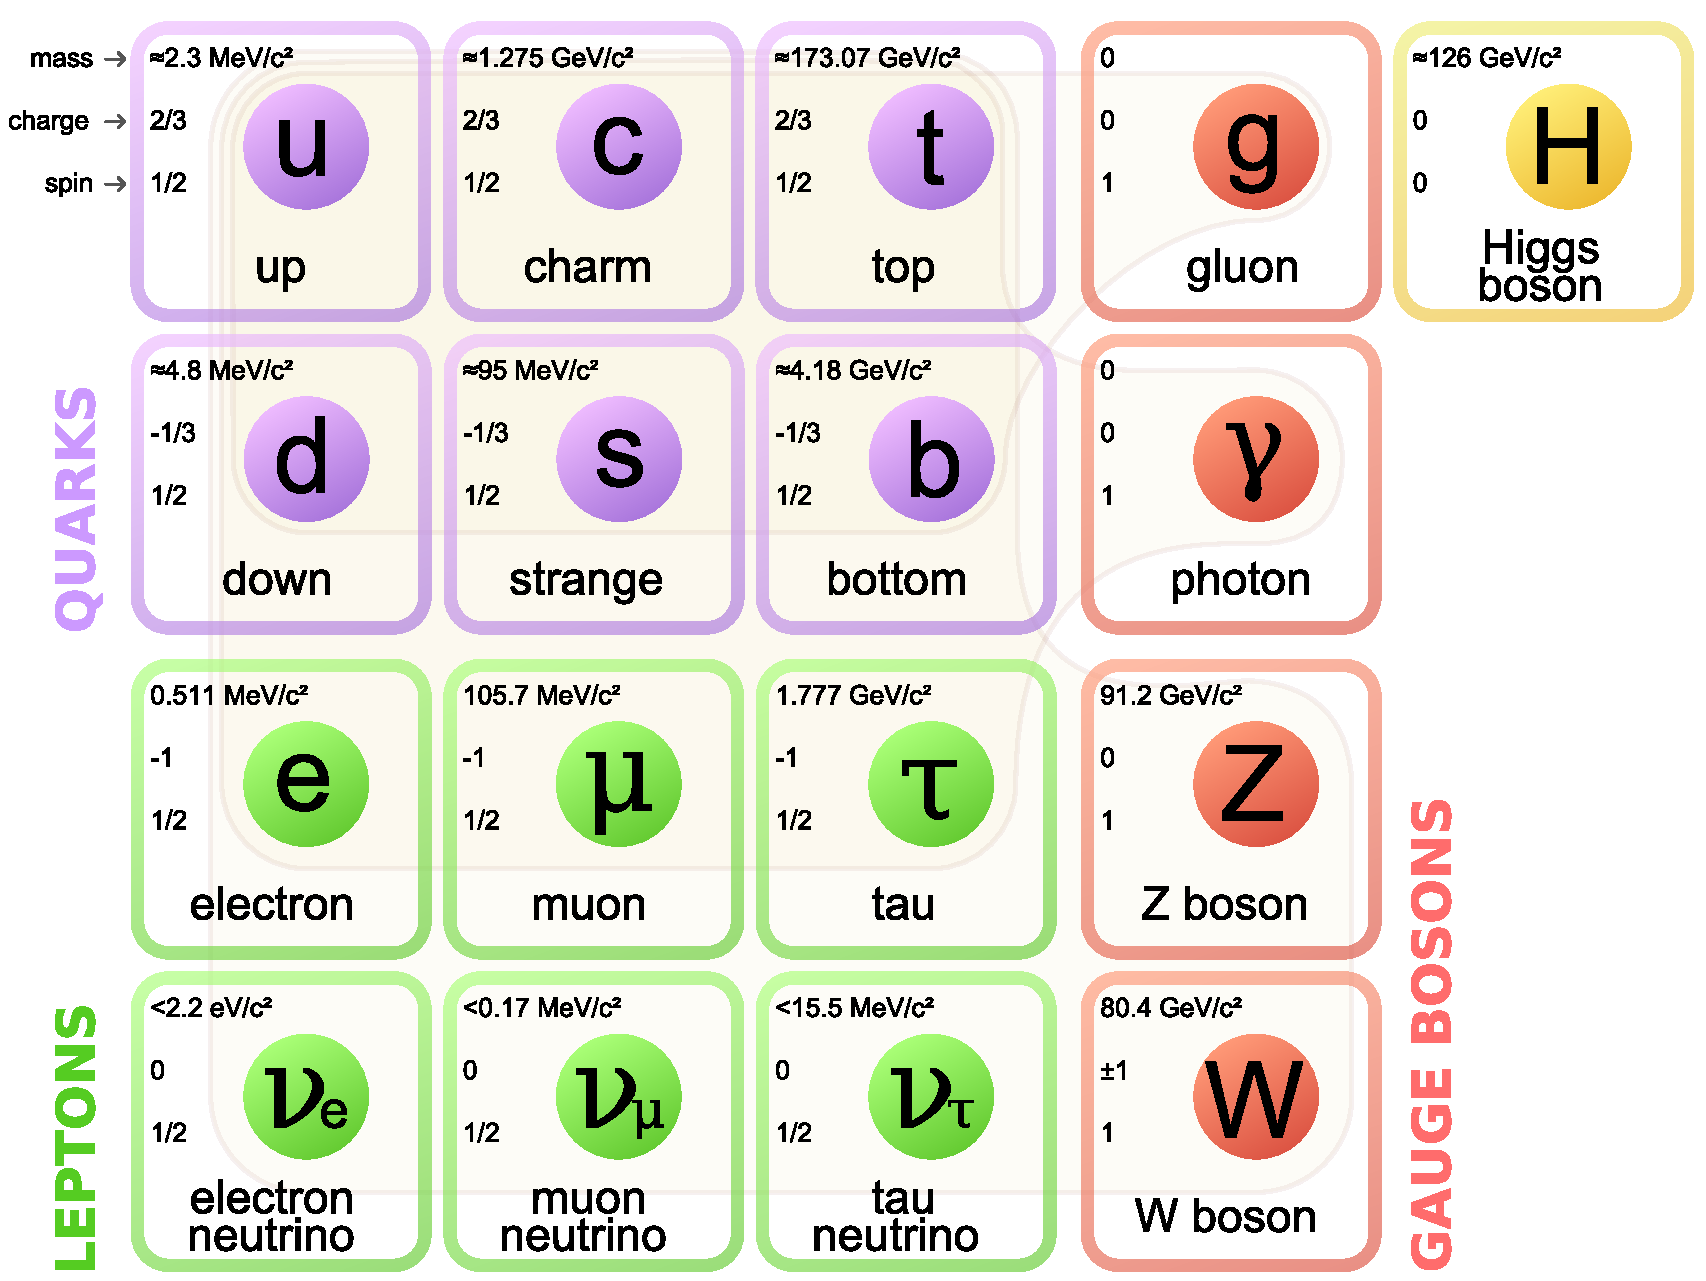
\includegraphics[width=0.95\textwidth]{figures/Standard_Model_of_Elementary_Particles.pdf}
\caption{A table of all the elementary particles in the standard model, with the spin, electric charge, and mass values of each particle \cite{MissMJ}. The faint gray lines indicate which gauge bosons interact with which fermions.}
\label{fig:sm-particles}
\end{center}
\end{figure}

The electromagnetic force is mediated by photons ($\gamma$), spin-1 gauge bosons which have no mass or electric charge $Q$. This force causes interactions between electrically charged particles and has infinite range due to the masslessness of the photon. Quantum electrodynamics (QED) is the quantum field theory description of electromagnetism, which can be represented by a $U(1)$ symmetry group. The weak force is mediated by the massive \Wpm and \Z bosons and can be represented by an $SU(2)$ symmetry group. The weak force acts on particles carrying weak isospin $T$. Weak isospin is a quantum number whose third component $T_3$ is conserved in all interactions and which can be mathematically treated in the same way as angular momentum, though the two quantities are physically distinct. The massiveness of the weak carrier bosons means that the weak force has a limited range, approximately $10^{-18}\unit{m}$. The charged current weak interaction, mediated by the \Wpm bosons, is sensitive to the chirality of fermions; only left-handed fermions and right-handed antifermions participate in this interaction. The neutral current weak interaction, mediated by the \Z boson, is not sensitive to chirality.

As suggested by the inclusion of both forces in the previous paragraph, the electromagnetic and weak forces can be unified to form the electroweak force, represented by the symmetry group $SU(2) \times U(1)$. In this unification, the quantum numbers of electromagnetism and the weak force are related by a new conserved quantum number, weak hypercharge $Y = 2(Q - T_3)$. The Higgs mechanism is responsible for electroweak symmetry breaking (EWSB). In order for the electroweak theory to be gauge invariant, the gauge bosons must be massless, but the \Wpm and \Z bosons are observed to have mass. The Higgs mechanism solves this dilemma via spontaneous EWSB due to its non-zero vacuum expectation value (VEV). The Higgs field consists of a doublet, with two charged particles and two neutral particles, all scalar bosons. The two charged particles and one of the neutral particles act as Goldstone bosons, combining with the \Wpm and \Z bosons to produce their masses. The remaining neutral particle is the Higgs boson, which was discovered at the LHC in 2012 \cite{NewBoson}.

The strong force, quantum chromodynamics (QCD), is mediated by gluons (\cPg) and can be represented by an $SU(3)$ symmetry group. Gluons, like photons, are spin-1 gauge bosons without mass or electric charge. However, gluons do possess color charge, the quantum number on which the strong force acts. Color charge is so named because the charge has three possible values, which are labeled red, green, or blue. Because gluons both mediate and participate in the strong interaction, the force between quarks does not decrease as they become spatially separated. The energy in the gluon field between the separated quarks can become large enough to form one or more quark-antiquark pairs. This phenomenon is known as confinement and prevents quarks or gluons from existing in a bare state. Correspondingly, the range of the strong force is limited to ${\sim} 10^{-15}\unit{m}$. Bound states of quarks and gluons, the only way they have ever been observed in nature, are called hadrons, and the formation of those bound states is called hadronization. States with one quark and one antiquark are mesons, while states with three quarks are baryons. Mesons and baryons are the two allowed types of bound states because they represent color singlets. Complementarily, as quarks get closer together, the strong force between them weakens. This behavior is known as asymptotic freedom; because short distances are equivalent to high energies, the strong interactions of quarks at a high-energy collider like the LHC can be calculated perturbatively. A residual form of the strong force acts on nucleons, protons and neutrons, to form atomic nuclei.

As mentioned, fermions are the particles of matter, which are separated into two groups: quarks and leptons. Quarks have fractional electric charge, weak isospin, and color charge, so they are affected by all three fundamental forces. There are two types of quarks: up-type quarks that have $Q = 2/3$ and down-type quarks that have $Q = -1/3$. Leptons consist of charged leptons and neutrinos. Charged leptons possess electric charge and weak isospin, while neutrinos only possess weak isospin. Three generations exist for each type of particle, with the different particles called flavors. The flavors of up-type quarks are the up, charm, and top quarks; of down-type quarks are the down, strange, and bottom quarks; of charged leptons are the electron, muon, and tau lepton; and of the neutrinos are the electron, muon, and tau neutrinos. The charged current weak interaction mixes the different flavors of quarks, with the amount of mixing between any two flavors given by the unitary Cabibbo-Kobayashi-Maskawa (CKM) matrix. The top quark is the heaviest elementary particle and is so heavy that it decays before hadronizing, making it an exception to the rule that bare quarks are not observed. Quarks possess an additively conserved quantum number called baryon number $B$, which is defined as $B = \frac{1}{3}(n_{\cPq} - n_{\overline{\cPq}})$. Similarly, lepton number $L$ is defined for leptons as $L = n_{\ell} - n_{\overline{\ell}}$. Specific lepton flavor numbers $L_{\Pe}$, $L_{\mu}$, $L_{\tau}$ are defined for each flavor pair of leptons.

The fermions are arranged into multiplets based on their chirality. The left-handed up- and down-type quarks are grouped together in a doublet $\cPq_L$, as are the left-handed charged leptons and neutrinos in $\ell_L$. The right-handed particles are singlets. It is important to note that right-handed neutrinos, and correspondingly left-handed antineutrinos, do not exist in the standard model. The Higgs field spontaneously provides masses to the quarks and charged leptons through a Yukawa interaction which couples the left- and right-handed versions of each flavor of particle. For a fermion $f$, this interaction takes the form $-y_{f} \overline{f}_{L} \PH f_{R}$, where $y_{f}$ is the Yukawa coupling. The quantum numbers of each type of particle are summarized in Table \ref{tab:q-num}, and the interactions among all the particles are illustrated in Fig. \ref{fig:sm-interactions}.

\begin{table}[htb]
  \begin{center}
%    \def\arraystretch{2.0} %1 is the default
    \begin{tabular}{|l||l|r|r|r|r|r|}
\hline
      & \multicolumn{1}{c|}{Particle} & \multicolumn{1}{c|}{$Q$} & \multicolumn{1}{c|}{$T_3$} & \multicolumn{1}{c|}{$Y$} & \multicolumn{1}{c|}{$B$} & \multicolumn{1}{c|}{$L$} \\
\hline
\hline
\multirow{3}{*}{Quarks}  
\rule{0pt}{24pt}         & $\cPq_L = \doublet[r]{\cPqu}{\cPqd}_L$ & $\doublet[r]{2/3}{-1/3}$ & $\doublet[r]{1/2}{-1/2}$ & $1/3$  & $1/3$ & 0 \\
                         & $\cPqu_R$                              & $2/3\hphantom{\bigg)}$   & $0\hphantom{\bigg)}$     & $4/3$  & $1/3$ & 0 \\
                         & $\cPqd_R$                              & $-1/3\hphantom{\bigg)}$  & $0\hphantom{\bigg)}$     & $-2/3$ & $1/3$ & 0 \\
\hline
\hline
\multirow{2}{*}{Leptons} 
\rule{0pt}{24pt}         & $\ell_L = \doublet[r]{\nu}{\Pe}_L$     & $\doublet[r]{0}{-1}$     & $\doublet[r]{1/2}{-1/2}$ & $-1$   & 0     & 1 \\
                         & $\Pe_R$                                & $-1\hphantom{\bigg)}$    & $0\hphantom{\bigg)}$     & $-2$   & 0     & 1 \\
\hline
    \end{tabular}
    \caption{The quantum numbers of each category of fermions, based on chirality and particle type: up-type quarks, down-type quarks, charged leptons, and neutrinos. The various flavors of each category, also called the first, second, and third generations of matter, possess the same quantum numbers and differ only in their masses.}
    \label{tab:q-num}
  \end{center}
\end{table}

\begin{figure}[hbt]
\begin{center}
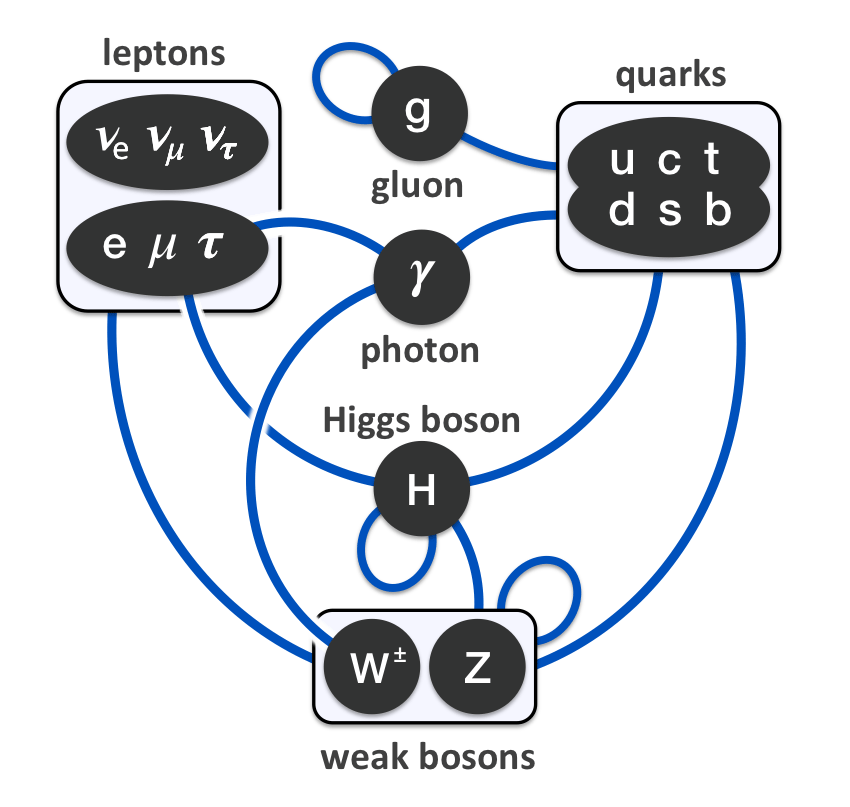
\includegraphics[width=0.95\textwidth]{figures/Elementary_particle_interactions_in_the_Standard_Model.png}
\caption{A diagram illustrating the leading order interactions between particles in the standard model, including self-interactions \cite{Drexler}.}
\label{fig:sm-interactions}
\end{center}
\end{figure}

%\addtocounter{section}{-1}
\renewcommand{\thesection}{\thechapter.{$\frac{1}{2}$}}
\section{Beyond the Standard Model}
\newcounter{sectionprime}
\addtocounter{sectionprime}{\value{section}}
\addtocounter{sectionprime}{-1}
\renewcommand{\thesection}{\thechapter.\arabic{sectionprime}} % use offset numbering

The predictions of the standard model have been confirmed by decades of precise experimental tests. However, as an effective field theory, its domain of applicability is ultimately limited; at a high enough energy, the theory will break down. Further, the standard model is unable to account for some observations. These limitations and indications of new phenomena motivate various searches for physics beyond the standard model (BSM), include the searches which will be presented in this dissertation.

The most obvious limitation of the standard model is that it depends on 19 free parameters which must be determined by experiment. These parameters include the nine fermion masses, the Higgs mass and VEV, the gauge couplings for the three forces, the three mixing angles and one phase from the CKM matrix, and finally the QCD vacuum angle. It is conceivable that a BSM theory could reduce the number of free parameters. Electroweak unification and charge quantization suggest that a Grand Unified Theory (GUT) could unify all three fundamental forces, at an expected energy scale of ${\sim} 10^{16}\GeV$. The observation of neutrino oscillations is now well established, indicating that neutrinos have small but non-zero masses. The oscillation of neutrinos between mass and flavor eigenstates is described by the Pontecorvo-Maki-Nakagawa-Sakata (PMNS) matrix. Like the CKM matrix for quarks, the PMNS matrix is unitary and has four parameters: three mixing angles and one phase. The values of the neutrino masses have not been directly measured, but are indirectly limited to the \eVns scale. Because right-handed neutrinos do not exist in the Standard Model, neutrinos cannot gain mass via a Yukawa interaction with the Higgs field. Though the Higgs mass is a parameter of the SM, it can be calculated in many BSM theories. Unless unnatural fine-tuning occurs, the presence of new massive particles makes this calculation produce a value near the Planck scale of $10^{19}\GeV$, orders of magnitude higher than the observed value of 125\GeV, which characterizes the electroweak scale. This is known as the hierarchy problem. To construct a natural theory which avoids such fine-tuning while making predictions that agree with observation, it is necessary to cancel divergent contributions to the Higgs mass. The hierarchy problem is an important motivation to search for new physics at the LHC \cite{Morrissey20121}.

Astrophysics provides numerous indications of the need for BSM theories. Most notably, gravity is not included in the standard model. A successful unification of general relativity and quantum field theory has not been achieved, due to the difficulty of constructing a renormalizable theory for the spin-2 graviton. At the Planck scale, gravitational effects become comparable to SM interactions, which calls for a new theory. The measurement of galactic rotation curves and galaxy cluster collisions \cite{BulletCluster} indicates that ${\sim} 85\%$ of the matter in the universe is dark matter, which interacts gravitationally but not electromagnetically. Dark matter is likely to be a new particle not present in the standard model. The most popular type of dark matter candidate is a weakly interacting massive particle (WIMP) \cite{Morrissey20121}, but many other candidates have been proposed. The dearth of antimatter relative to the amount of matter in the universe requires greater violation of charge-parity (CP) symmetry than is contained in the SM. The accelerating expansion of the universe, observed using standard candle supernovae \cite{Supernova98,Supernova99}, implies that ${\sim} 70\%$ of the energy of the universe exists in a unknown form called dark energy. Dark energy may be a result of the cosmological constant of the universe, which can be related to the energy of the vacuum in quantum field theory. However, the standard model predicts that this cosmological constant would be $10^{120}$ times larger than the observed value, a clear failure of the theory. The recent tentative evidence for cosmic inflation from the Background Imaging of Cosmic Extragalactic Polarization (BICEP) experiment \cite{BICEP} implies the existence of the inflaton, a new scalar field.

The following sections discuss the theories of leptoquarks and R-parity violating supersymmetry. The existence of leptoquarks can be a consequence of grand unification or other theories that address the parallels between leptons and quarks in the standard model. Supersymmetry is motivated by basic considerations of quantum field theory, the hierarchy problem, grand unification, and dark matter. The introduction of R-parity violation in supersymmetry evades existing limits on signatures with large missing transverse energy due to the stability of the lightest supersymmetric particle, while retaining some of the other desirable characteristics of supersymmetry. R-parity violating supersymmetry can also act as a signature generator to suggest novel searches which might discover or rule out other BSM theories \cite{EvansSigGen}.

\stepcounter{sectionprime}
\section{Leptoquarks
\label{sec:LQ}}

Many BSM theories include a deeper relationship between leptons and quarks. Such a relationship is indicated by the cancellation of SM gauge anomalies from triangle diagrams, which requires each generation of matter to consist of quarks and leptons with the specific weak hypercharge values and multiplet arrangements that they possess in the SM \cite{Peskin}. Such theories introduce a class of particles called leptoquarks (LQs), which possess lepton number, baryon number, color charge, and fractional electric charge. Leptoquarks are bosons, either scalar with spin 0 or vector with spin 1. The values of the LQ quantum numbers, including those listed previously as well as weak isospin, which they may or may not possess, are model-dependent. A total fermion number $F$ can be defined as $F = 3B + L$ to characterize the combinations of lepton and baryon numbers found in LQs. The possible values are $F=0$ for LQs which couple to $\overline{\ell}\cPq$ or $\ell\overline{\cPq}$ pairs and $|F|=2$ for coupling to $\ell\cPq$ or $\overline{\ell}\overline{\cPq}$ pairs.

The first BSM theory to include leptoquarks was Pati-Salam $SU(4)$ \cite{SU4}, a GUT which casts lepton number as the fourth type of color charge, hence the $SU(4)$ symmetry instead of the SM $SU(3)$. Another GUT, Georgi-Glashow $SU(5)$ \cite{GUT}, also contains leptoquarks. In general, grand unified theories group leptons and quarks together in multiplets. However, the symmetry breaking in these theories typically occurs at the GUT scale, rendering the expected LQ masses very large and therefore unable to be directly produced at colliders. $E_6$ superstring theory \cite{SUPERSTR} can also contain LQs, as it behaves similarly to GUTs below the string compactification scale, which is typically near the Planck scale. In other models, leptoquarks may be composite particles \cite{LQ3b}. These include extended technicolor theories \cite{TC3}, which postulate a new strong interaction similar to QCD and provide spontaneous masses to SM fermions using technifermions. A techniquark and anti-technilepton can bind together to form a technimeson which interacts with SM fermions as a leptoquark with a model-dependent coupling. Technicolor, though, has become disfavored with the confirmation of the Higgs mechanism for EWSB and fermion masses.

The Buchm\"{u}ller-R\"{u}ckl-Wyler (BRW) model of leptoquarks includes all renormalizable Lagrangian terms compatible with the standard model \cite{BRW}. There are several constraints imposed in the BRW model:
\begin{enumerate}
\item LQ interactions are dimensionless, in order to be renormalizable.
\item LQ interactions are invariant under the overall SM symmetry $SU(3) \times SU(2) \times U(1)$.
\item LQ interactions conserve $B$ and $L$, to avoid contributions to proton decay.
\item LQs couple only to SM particles.
\end{enumerate}
Further consideration of experimental limits imposes two additional constraints, creating the minimal BRW (mBRW) model:
\begin{enumerate}
\setcounter{enumi}{4}
\item LQ couplings are chiral, involving either only left-handed fermions or only right-handed fermions, due to limits on otherwise chirally-suppressed decays such as $\pi^{+} \rightarrow \Pe^{+} \nu_{\Pe}$.
\item LQ couplings involve only a single generation of leptons and quarks, to evade limits on flavor-changing neutral currents (FCNCs).
\end{enumerate}
The Lagrangian terms are given for scalar LQs in Eq. \eqref{eq:Lagrangian-SLQ} and for vector LQs in Eq. \eqref{eq:Lagrangian-VLQ} below, using the ``Aachen'' notation as specified in Ref. \cite{ModelIndLQ}.
\begin{align}
\label{eq:Lagrangian-SLQ}
\mathcal{L}_{S} = &\hphantom{+~}(\lambda_{L,S_{0}} \overline{\cPq}_{L}^{c} i\sigma_{2} \ell_{L} + \lambda_{R,S_{0}} \overline{\cPqu}_{R}^{c} \Pe_{R})S_{0}^{\dagger}
+ \lambda_{R,\widetilde{S}_{0}} \overline{\cPqd}_{R}^{c} \Pe_{R} \widetilde{S}_{0}^{\dagger} \nonumber \\
&+ (\lambda_{L,S_{1/2}} \overline{\cPqu}_{R} \ell_{L} + \lambda_{R,S_{1/2}} \overline{\cPq}_{L} i\sigma_{2} \Pe_{R})S_{1/2}^{\dagger}
+ \lambda_{L,\widetilde{S}_{1/2}} \overline{\cPqd}_{R} \ell_{L} \widetilde{S}_{1/2}^{\dagger} \nonumber \\
&+ \lambda_{L,S_{1}} \overline{\cPq}_{L}^{c} i\sigma_{2}\boldsymbol{\sigma} \ell_{L} \cdot \boldsymbol{S}_{1}^{\dagger} + \text{h.c.} \\
%\end{align}
%\begin{align}
\label{eq:Lagrangian-VLQ}
\mathcal{L}_{V} = &\hphantom{+~}(\lambda_{L,V_{0}} \overline{\cPq}_{L} \gamma_{\mu} \ell_{L} + \lambda_{R,V_{0}} \overline{\cPqd}_{R} \gamma_{\mu} \Pe_{R})V_{0}^{\mu\dagger}
+ \lambda_{R,\widetilde{V}_{0}} \overline{\cPqu}_{R} \gamma_{\mu} \Pe_{R} \widetilde{V}_{0}^{\mu\dagger} \nonumber \\
&+ (\lambda_{L,V_{1/2}} \overline{\cPqd}_{R}^{c} \gamma_{\mu} \ell_{L} + \lambda_{R,V_{1/2}} \overline{\cPq}_{L}^{c} \gamma_{\mu} \Pe_{R})V_{1/2}^{\mu\dagger}
+ \lambda_{L,\widetilde{V}_{1/2}} \overline{\cPqu}_{R}^{c} \gamma_{\mu} \ell_{L} \widetilde{V}_{1/2}^{\mu\dagger} \nonumber \\
&+ \lambda_{L,V_{1}} \overline{\cPq}_{L} \gamma_{\mu}\boldsymbol{\sigma} \ell_{L} \cdot \boldsymbol{V}_{1}^{\mu\dagger} + \text{h.c.}
\end{align}
In these equations, scalar leptoquarks are denoted by $S$ and vector leptoquarks are denoted by $V$. The subscripts 0, 1/2, and 1 denote singlet, doublet, and triplet states, respectively. The $\widetilde{S}$ and $\widetilde{V}$ leptoquarks have different quantum numbers compared to the corresponding $S$ and $V$ leptoquarks. The coupling constants for the Yukawa couplings between leptoquarks, leptons, and quarks are represented by $\lambda$, with the chirality $L$ or $R$ and the leptoquark type indicated in the subscript. The generation indices for the couplings and fermion multiplets are suppressed. The Pauli matrices are denoted by $\sigma_{i}$ and the Dirac matrices by $\gamma_{\mu}$. The Hermitian conjugate terms are indicated as ``h.c.'' The quantum numbers for the different types of mBRW leptoquarks are listed in Table \ref{tab:lq-num}.

\begin{table}[htb]
  \begin{center}
%    \def\arraystretch{3.0} %1 is the default
    \begin{tabular}{|l||l|r|r|r|r|}
\hline
      & \multicolumn{1}{c|}{Particle} & \multicolumn{1}{c|}{$Q$} & \multicolumn{1}{c|}{$T_3$} & \multicolumn{1}{c|}{$Y$} & \multicolumn{1}{c|}{$F$} \\
\hline
\hline
\multirow{10}{*}{Scalar} & $S_{0}$               & $-1/3\hphantom{\bigg)}$                            & $0\hphantom{\bigg)}$                              & $-2/3$ & $2$ \\
                         & $\widetilde{S}_{0}$   & $-4/3\hphantom{\bigg)}$                            & $0\hphantom{\bigg)}$                              & $-8/3$ & $2$ \\
\rule{0pt}{24pt}         & $S_{1/2}$             & $\doublet[r]{-2/3}{-5/3}$ & $\doublet[r]{1/2}{-1/2}$ & $-7/3$ & $0$ \\
\rule{0pt}{24pt}         & $\widetilde{S}_{1/2}$ & $\doublet[r]{1/3}{-2/3}$  & $\doublet[r]{1/2}{-1/2}$ & $-1/3$ & $0$ \\
\rule{0pt}{36pt}         & $S_{1}$               & $\triplet[r]{2/3}{-1/3}{-4/3}$       & $\triplet[r]{1\vphantom{/}}{0\vphantom{/}}{-1\vphantom{/}}$             & $-2/3$ & $2$ \\
\hline
\hline
\multirow{10}{*}{Vector} & $V_{0}$               & $-2/3\hphantom{\bigg)}$                            & $0\hphantom{\bigg)}$                              & $-4/3$  & $0$ \\
                         & $\widetilde{V}_{0}$   & $-5/3\hphantom{\bigg)}$                            & $0\hphantom{\bigg)}$                              & $-10/3$ & $0$ \\
\rule{0pt}{24pt}         & $V_{1/2}$             & $\doublet[r]{-1/3}{-4/3}$ & $\doublet[r]{1/2}{-1/2}$ & $-5/3$  & $2$ \\
\rule{0pt}{24pt}         & $\widetilde{V}_{1/2}$ & $\doublet[r]{2/3}{-1/3}$  & $\doublet[r]{1/2}{-1/2}$ & $1/3$   & $2$ \\
\rule{0pt}{36pt}         & $V_{1}$               & $\triplet[r]{1/3}{-2/3}{-5/3}$       & $\triplet[r]{1\vphantom{/}}{0\vphantom{/}}{-1\vphantom{/}}$             & $-4/3$  & $0$ \\
\hline
    \end{tabular}
    \caption{The quantum numbers of the different types of scalar and vector leptoquarks in the mBRW model.}
    \label{tab:lq-num}
  \end{center}
\end{table}

As color-charged particles, leptoquarks are primarily produced by strong interactions in $\Pp\Pp$ collisions. For pair production of leptoquarks, these interactions include gluon-gluon fusion and quark-antiquark annihilation, whose LO forms are shown in Fig. \ref{fig:lq-diagrams}. An additional contribution to quark-antiquark annihilation may proceed through the Yukawa coupling $\lambda$ of the leptoquark to the quark and lepton pair. However, the ratio $\MLQ/\lambda$, where $\MLQ$ is the leptoquark mass, is restricted by limits from low-energy processes including $\pi^{+} \rightarrow \Pe^{+} \nu_{\Pe}$ and atomic parity violation. The limits on $\MLQ/\lambda$ range from 1800--6400\GeVcc, depending on the type of leptoquark \cite{Leurer:1993em, MuchAdo, LQreview}. The expected accessible mass range for leptoquarks at the LHC with $\sqrt{s}=14\TeV$ ranges from 900--1200\GeVcc for scalar LQs and 1200--1500\GeVcc for vector LQs, depending on the desired number of events \cite{LQPairHad}. Up to these masses, $\lambda$ will be small enough that its contribution to leptoquark production can be neglected. This applies both to the Yukawa-based pair production diagram in Fig. \ref{fig:lq-diagrams} and the single production diagrams from quark-gluon scattering in Fig. \ref{fig:lq-single}.

\begin{figure}[hbt]
\begin{center}
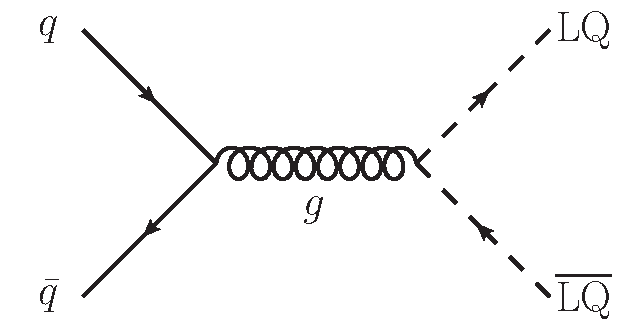
\includegraphics[width=0.49\textwidth]{figures/LO_FD_LQ_pair_a.pdf}
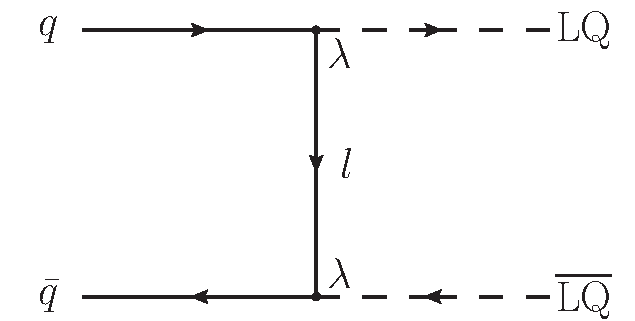
\includegraphics[width=0.49\textwidth]{figures/LO_FD_LQ_pair_b.pdf}
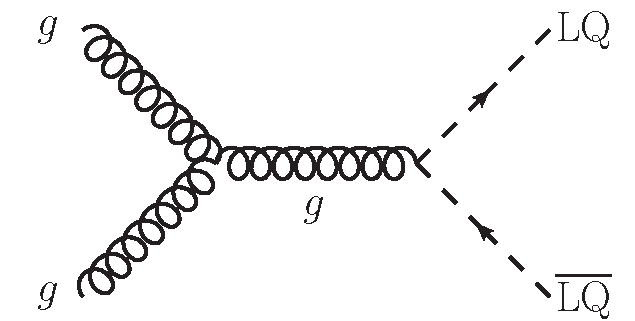
\includegraphics[width=0.49\textwidth]{figures/LO_FD_LQ_pair_c.pdf}
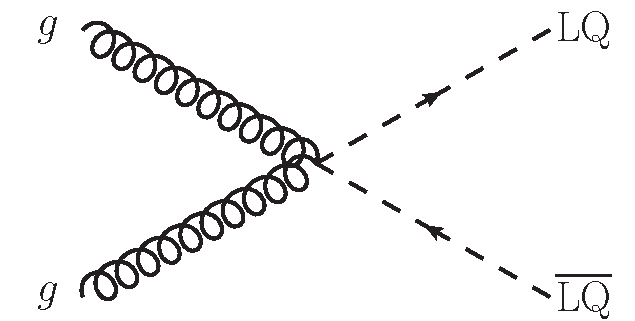
\includegraphics[width=0.49\textwidth]{figures/LO_FD_LQ_pair_d.pdf}
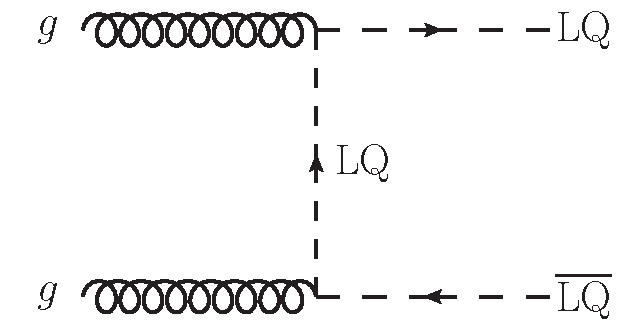
\includegraphics[width=0.49\textwidth]{figures/LO_FD_LQ_pair_e.pdf}
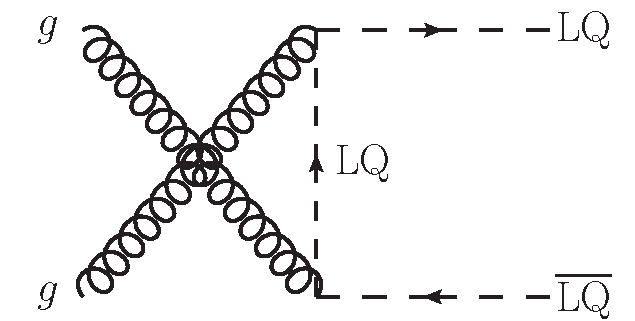
\includegraphics[width=0.49\textwidth]{figures/LO_FD_LQ_pair_f.pdf}
\caption{The LO diagrams for leptoquark pair production from quark-antiquark annihilation (top) and gluon-gluon fusion (middle, bottom).}
\label{fig:lq-diagrams}
\end{center}
\end{figure}

\begin{figure}[hbt]
\begin{center}
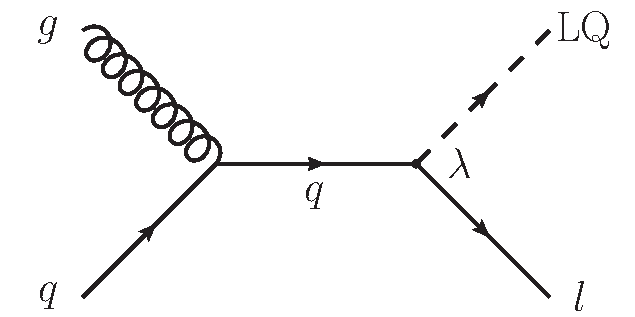
\includegraphics[width=0.49\textwidth]{figures/LO_FD_single_LQ_a.pdf}
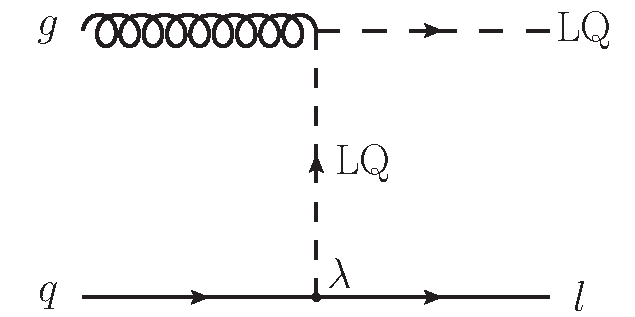
\includegraphics[width=0.49\textwidth]{figures/LO_FD_single_LQ_b.pdf}
\caption{The LO diagrams for single leptoquark production from quark-gluon scattering. The LQ is produced in association with a lepton.}
\label{fig:lq-single}
\end{center}
\end{figure}

Table \ref{tab:lq-xsec} lists the pair production cross sections for a range of scalar leptoquark masses. They have been calculated using the CTEQ6 parton distribution functions (PDFs) \cite{CTEQ6r1,CTEQ6r2} with $K$-factors applied to include NLO corrections from QCD \cite{LQxsec}. Theoretical uncertainties are calculated by propagating the PDF uncertainty and varying the factorization/renormalization scale $\mu$. These cross sections are sensitive only to the leptoquark mass and spin, so they are largely model-independent. For vector leptoquarks, the cross sections may be modified by anomalous triple and quartic gauge couplings. The decay widths for scalar and vector leptoquarks can be calculated according to Eqs. \eqref{eq:SLQ-width} and \eqref{eq:VLQ-width}, respectively \cite{BRW}:
\begin{align}
\label{eq:SLQ-width} \Gamma_{S} &= \sum_{i}{\frac{\lambda_{i}^{2}}{16\pi}\MLQ}, \\
\label{eq:VLQ-width} \Gamma_{V} &= \sum_{i}{\frac{\lambda_{i}^{2}}{24\pi}\MLQ}.
\end{align}
Equations \eqref{eq:SLQ-width} and \eqref{eq:VLQ-width} sum over all Yukawa couplings for a given leptoquark. Given the limits on $\lambda$ discussed above, leptoquarks accessible at the LHC with a single Yukawa coupling can be expected to have a fractional decay width of less than 0.1--0.2\%.

\begin{table}[htb]
\begin{center}
{\footnotesize
\begin{tabular}{|l||c|c||c|c|}
\hline
$\MLQ$ & $\sigma (\mu = \MLQ)$ & $\delta (\text{PDF}) $ & $\sigma (\mu = \MLQ/2)$ & $\sigma (\mu = 2\MLQ)$ \\
\hline
\hline
 200 & 17.4 & 1.24 & 15.0 & 19.7  \\
 250 & 5.26 & 0.487 & 4.54 & 5.94  \\
 300 & 1.89 & 0.214 & 1.63 & 2.13  \\
 350 & 0.77 & 0.102 & 0.663 & 0.866  \\
 400 & 0.342 & 0.052 & 0.295 & 0.385  \\
 450 & 0.163 & 0.0278 & 0.14 & 0.183  \\
 500 & 0.082 & 0.0155 & 0.0704 & 0.0922  \\
 550 & 0.0431 & 0.00893 & 0.037 & 0.0485  \\
 600 & 0.0235 & 0.0053 & 0.0201 & 0.0265  \\
 650 & 0.0132 & 0.00322 & 0.0113 & 0.0149  \\
 700 & 0.00761 & 0.002 & 0.00648 & 0.00858  \\
 750 & 0.00448 & 0.00126 & 0.00381 & 0.00506  \\
 800 & 0.00269 & 0.00081 & 0.00228 & 0.00304  \\
 850 & 0.00164 & 0.000527 & 0.00139 & 0.00186  \\
 900 & 0.00101 & 0.000347 & 0.000856 & 0.00115  \\
 950 & 0.000634 & 0.000231 & 0.000534 & 0.000722  \\
 1000 & 0.000401 & 0.000155 & 0.000337 & 0.000458  \\
\hline
\end{tabular}
}
\caption{The pair production cross sections for a range of scalar leptoquark masses at $\sqrt{s}=8\TeV$. Theoretical uncertainties from the PDFs and from varying the factorization/renormalization scale $\mu$ from $\mu=\MLQ/2$ to $\mu=2\MLQ$ are indicated.}
\label{tab:lq-xsec}
\end{center}
\end{table}

In this dissertation, a search is performed for pair production of scalar leptoquarks decaying to third generation fermions. The symbol $\mathcal{B}$ is used for the branching fraction for the decay $\text{LQ} \rightarrow \tau \cPqb$. This results a final state with two tau leptons and two bottom quarks. One tau lepton is required to decay leptonically: $\tau \rightarrow \ell \overline{\nu_{\ell}} \nu_{\tau}$, where $\ell$ can be a muon or an electron, which are collectively called light leptons. The other tau lepton is required to decay hadronically, denoted as \tauh; see Sec. \ref{sec:hpstau} for more information about hadronic decays of tau leptons. These decays result in two channels based on the leptonic decay of the tau, which are labeled as \etau and \mutau, or collectively \ltau when the light lepton flavor is unimportant. Both bottom quarks hadronize into b-jets, as described in Sec. \ref{sec:b-tagging}. Currently, the strongest mass limits on such third-generation scalar leptoquarks come from direct searches. Assuming $\mathcal{B}=100\%$, the lower limit is approximately 530\GeV, set by both the CMS \cite{CMSLQ3} and ATLAS \cite{ATLASLQ3} experiments using 4.7--4.8\fbinv of data from $\Pp\Pp$ collisions with $\sqrt{s}=7\TeV$. Indirect limits from low-energy processes are discussed in Refs. \cite{ModelIndLQ,Leurer:1993em, MuchAdo, LQreview}.

%talk about reinterpreted search to cover low B?

\stepcounter{sectionprime}
\section{R-Parity Violating Supersymmetry
\label{sec:RPVSUSY}}

At the most basic level, supersymmetry proposes a symmetry between bosons and fermions. Such a symmetry appeals to mathematical considerations in quantum field theory by simplifying many calculations \cite{Peskin}. However, the primary motivation for a theory of SUSY with effects at the electroweak scale and therefore accessible at the LHC is the hierarchy problem. The mass of the Higgs boson, experimentally measured as $M_{\PH} = 125\GeV$, is theoretically sensitive to quantum corrections via loop diagrams from any particle that couples to it. This sensitivity makes the experimentally-measured value highly suspicious. Precise cancellations must occur among the various quantum corrections to produce such a small mass value, relative to the expected energy scales of new physics. Any BSM theory lacking a simple mechanism to produce such cancellations must undergo unnatural fine-tuning in order to arrive at the correct value of $M_{\PH}$. The following discussion of supersymmetry is drawn primarily from Ref. \cite{Primer}.

The Higgs mass parameter $m_{\PH}^{2}$ appears in the Higgs potential:
\begin{equation}
V = m_{\PH}^{2}|\PH|^{2} + \lambda_{\PH}|\PH|^{4}.
\end{equation}
Consider the one-loop contribution to $m_{\PH}^{2}$ from a fermion $f$ which has a Yukawa coupling to the Higgs field, $-y_{f} \overline{f}_{L} \PH f_{R}$. The correction term in the mass parameter calculation can be written as follows:
\begin{equation}
\Delta_{f} m_{\PH}^{2} = -\frac{|y_{f}|^{2}}{8\pi^{2}}\Lambda_{\text{UV}}^{2} + \cdots. \label{eq:DMH-fermion}
\end{equation}
The factor $\Lambda_{\text{UV}}$ is the cutoff scale used to handle the ultraviolet divergence in the loop integral through regularization. This cutoff scale is typically related to the energy scale of new physics, e.g. the GUT scale or Planck scale. Even if the cutoff scale is small, the contribution to the Higgs mass from any new heavy fermion will be proportional to its Yukawa coupling $y$, which could itself be large. Similarly, consider the one-loop contribution from a scalar boson $S$ with a coupling to the Higgs written as $-y_{S} |\PH|^{2} |S|^{2}$, which produces a correction term:
\begin{equation}
\Delta_{S} m_{\PH}^{2} = \frac{y_{S}}{16\pi^{2}}\Lambda_{\text{UV}}^{2} + \cdots. \label{eq:DMH-scalar}
\end{equation}
Both one-loop diagrams are shown in Fig. \ref{fig:higgs-cancel}. The leading terms of Eqs. \eqref{eq:DMH-fermion} and \eqref{eq:DMH-scalar} have opposite signs, which suggests that the two terms could cancel if there were two scalars for each fermion, with $y_{S} = |y_{f}|^2$.

\begin{figure}[hbt]
\begin{center}
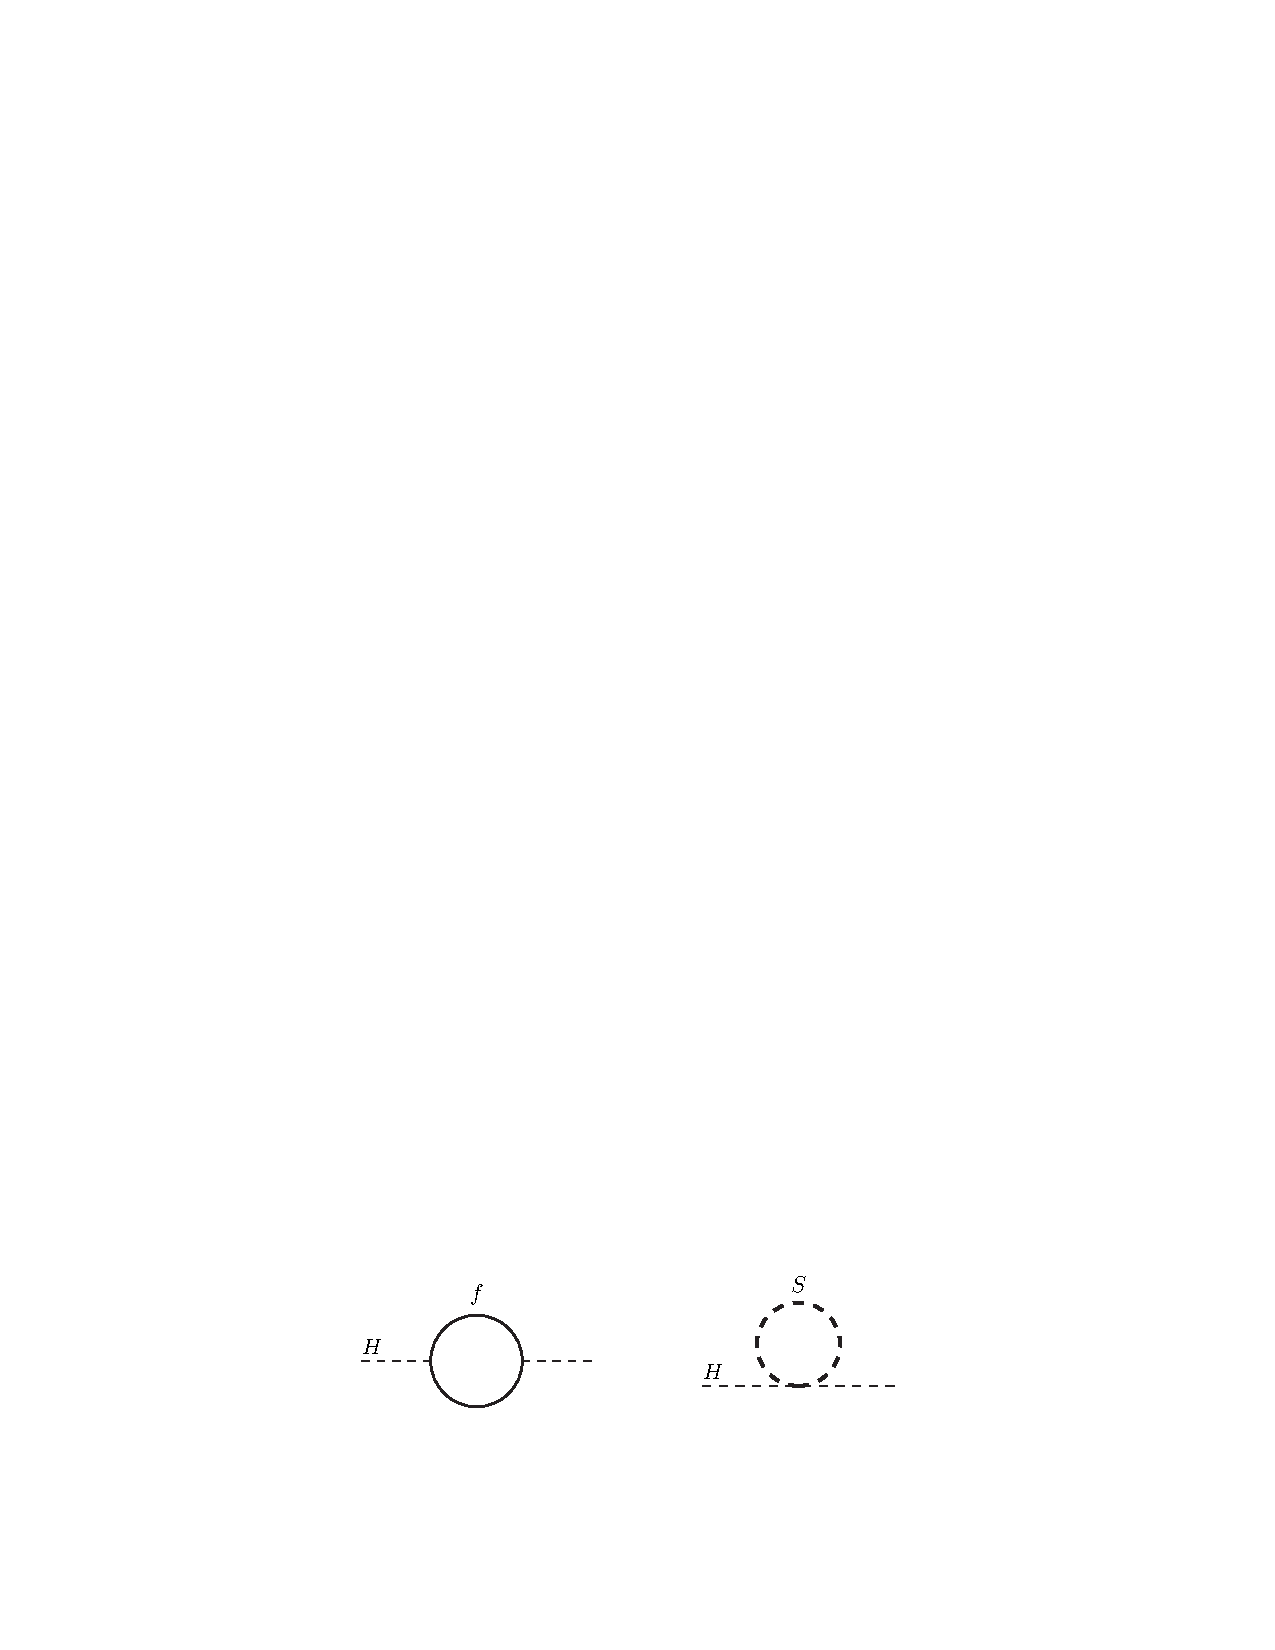
\includegraphics[width=0.95\textwidth]{figures/9709356v6-higgs-cancel.pdf}
\caption{One-loop diagrams for contributions to the Higgs mass parameter $m_{\PH}^{2}$ from a fermion $f$ (left) and a scalar $S$ (right) \cite{Primer}.}
\label{fig:higgs-cancel}
\end{center}
\end{figure}

This observation motivates SUSY as an extension of the standard model. While many formulations of SUSY exist, it is instructive to consider the minimal supersymmetric model (MSSM) to understand the fundamental components of the class of SUSY theories. SM particles are paired with new particles called superpartners with a spin difference of 1/2; SM fermions have scalar boson superpartners and SM bosons have spin-1/2 fermion superpartners. The scalar superpartners are named after the corresponding SM fermions with the prefix ``s-'', e.g. squarks and sleptons. The fermionic superpartners are named after the corresponding SM bosons with the suffix ``-ino'', e.g. higgsinos and gauginos. The symbols for superpartners are indicated by a tilde $\widetilde{\hphantom{H}}$. SM particles and their superpartners are arranged together in supermultiplets which extend the multiplets listed in Table \ref{tab:q-num}. Chiral supermultiplets contain scalar bosons and spin-1/2 fermions, while gauge supermultiplets contain spin-1/2 fermions and vector bosons. The superpartners possess the same quantum numbers as the corresponding SM particles, except for spin.

The Higgs boson, as a scalar, therefore becomes part of a chiral supermultiplet with weak hypercharge values $Y = \pm 1/2$. However, the existence of such chiral higgsinos creates new triangle gauge anomalies which must be cancelled to preserve the consistency of the theory. In addition, the weak hypercharge values of the Higgs supermultiplet restrict the possible Yukawa interactions with the other chiral supermultiplets, which are necessary for spontaneous fermion masses. For both of these reasons, the MSSM contains two Higgs doublets, conventionally labeled \Hone and \Htwo to indicate their couplings to up-type quarks or down-type quarks and charged leptons, respectively. Each Higgs doublet has its own VEV, labeled $v_{\cPqu}$ and $v_{\cPqd}$, which are considered to be two components of an underlying $v$, implying an angle $\beta$ can be defined as $\text{tan}(\beta) = v_{\cPqu}/v_{\cPqd}$.

Given these details, the superpotential of the MSSM, $W_{\text{MSSM}}$, contains these terms:
\begin{equation}
W_{\text{MSSM}} = y_{\cPqu,ij}\PU_{i}^{c}\PQ_{j}\Hone + y_{\cPqd,ij}\PD_{i}^{c}\PQ_{j}\Htwo + y_{\Pe,ij}\PE_{i}^{c}\PL_{j}\Htwo + \mu \Hone \Htwo. \label{eq:WMSSM}
\end{equation}
Equation \eqref{eq:WMSSM} is written in terms of superfields. $\PU$ is the up-type quark singlet superfield; $\PD$ is the down-type quark singlet superfield; $\PQ$ is the quark doublet superfield; $\PE$ is the charged lepton singlet superfield; and $\PL$ is the lepton doublet superfield. The Yukawa couplings $y$ are labeled by the fermion type $\cPqu$, $\cPqd$, or $\Pe$ with generation indices $i$, $j$. As an example, the top quark Yukawa coupling is $y_{\cPqu,33} = y_{\cPqt}$. The higgsino mass parameter is denoted as $\mu$.

The superpotential is limited to these terms by requiring the conservation of $R$-parity. The quantity $R$ is related to the baryon and lepton numbers as well as the particle spin $S$ and may be defined in two equivalent ways \cite{Barbier}, as shown in Eq. \eqref{eq:Rdef}. Equation \eqref{eq:Rparity} defines $R$-parity based on $R$.
\begin{align}
R &= 3B+L+2S = 3(B-L)+2S, \label{eq:Rdef} \\
R_{p} &= (-1)^{R}. \label{eq:Rparity}
\end{align}
All SM particles have $R_{p} = +1$, while all superpartners have $R_{p} = -1$. If $R$-parity is conserved, interactions which violate lepton or baryon number are not allowed. Notably, there must necessarily be a lightest supersymmetric particle (LSP) that is stable in order to conserve $R$-parity in the decay of any SUSY particle. In many models, the LSP is the lightest neutralino, a state created by mixing between the neutral higgsinos and gauginos due to EWSB. As a weakly interacting massive particle, the neutralino LSP is a promising candidate for WIMP dark matter.

If supersymmetry were unbroken, superpartners would have the same masses as their corresponding SM particles and would already have been detected. Therefore, there must be some mechanism responsible for breaking supersymmetry. In order for broken SUSY to continue to solve the hierarchy problem, it must preserve the conditions such as $y_{S} = |y_{f}|^2$ that lead to natural cancellations in the Higgs mass correction terms. So-called ``soft'' supersymmetry breaking accomplishes this by separating the Lagrangian into two separate terms:
\begin{equation}
\mathcal{L} = \mathcal{L}_{\text{SUSY}} + \mathcal{L}_{\text{soft}},
\end{equation}
where $\mathcal{L}_{\text{SUSY}}$ is made up of the SUSY-preserving terms, including the Yukawa interactions from the superpotential as well as the gauge interactions, and $\mathcal{L}_{\text{soft}}$ is made up of the SUSY-violating terms. The contributions to $\mathcal{L}_{\text{soft}}$ must be only mass terms and couplings whose parameters have positive mass dimension. These include interactions between three scalars, two sfermions and a Higgs, such as $a_{\cPqu,ij} \sUp_{i}^{c} \sQua_{j} \Hone$, where $a_{\cPqu,ij}$ are the soft couplings for those interactions. All such soft couplings are either at or below the mass scale $m_{\text{soft}}$, which is expected to be around the TeV scale from hierarchy problem considerations.

In general, the soft SUSY breaking terms can introduce FCNCs and CP violation that are strictly limited by precision measurements. This can be avoided by assuming the sfermion masses are universal; in other words, all sfermions should have the same mass regardless of flavor. This ``flavor-blindness'' eliminates mixing between flavors, and as a bonus, greatly reduces the number of free parameters in the MSSM. For first- and second-generation sfermions, flavor-blind universal masses are the norm. However, in the third generation, the sfermion masses can differ from the other two generations. In SUSY calculations, the couplings and mass parameters are treated as running factors which change based on renormalization group (RG) equations. These RG equations lead to corrections which tend to be small for Yukawa interactions, except for third generation particles which have relatively large Yukawa couplings. The effects of RG evolution in SUSY on the gauge couplings for the three fundamental forces significantly aid grand unification, which is another motivation for SUSY.

The concept of naturalness, described in Ref. \cite{NaturalSUSY}, indicates that the third-generation sfermion masses should in fact be significantly lighter than the other superpartners. The tree level relationship $M_{\Z}^{2} \propto |\mu|^{2} + |m_{\Hone}^{2}|$ implies that the superpartners with the largest contributions to $\mu$ and $m_{\Hone}^{2}$ must have masses near the electroweak scale. This applies especially to the higgsinos due to their involvement with $\mu$ and to the top squark which generates the largest correction to $m_{\Hone}^{2}$. To some extent, the other third-generation sfermions and the gluino are also affected by this consideration. In addition, because the top squark masses are not flavor-blind, the mass eigenstates can involve significant mixing between the chiral eigenstates. The top squark mass matrix is written as follows:
\begin{equation}
\mathbf{m_{\sTop}^{2}} =
\begin{pmatrix}
m_{\PQ 3}^{2} + m_{\cPqt}^{2} + \Delta_{\sUp_{L}} & v(a_{\cPqt}^{\ast}\text{sin}(\beta) - \mu y_{\cPqt}\text{cos}(\beta)) \\
v(a_{\cPqt}\text{sin}(\beta) - \mu^{\ast} y_{\cPqt}\text{cos}(\beta)) & m_{\PU 3}^{2} + m_{\cPqt}^{2} + \Delta_{\sUp_{R}}
\end{pmatrix}.
\end{equation}
The terms $\Delta_{\sUp_{L}}$ and $\Delta_{\sUp_{R}}$ arise via hyperfine splitting from quartic interactions and are defined in Ref. \cite{Primer}. When this mass matrix is diagonalized, a large mixing angle typically occurs because of the off-diagonal entries, which contain terms involving the large top Yukawa coupling and soft coupling. This means that one top squark mass eigenstate will be lighter than the other, and in fact it will be the lightest squark. This mass splitting, together with the general consideration of naturalness that implies a light top squark mass, suggests that top squarks are likely to be accessible at the LHC.

In $R$-parity conserving (RPC) SUSY, all decays of superpartners eventually produce at least one LSP. As a weakly interacting particle, the LSP will escape a particle detector without being detected, leading to events with signatures including large missing transverse energy or \met. The precise details of the production and decay of SUSY particles depend on which model is considered. This section has focused on the MSSM, but many variations of this model exist. These include, but are not limited to \cite{PDG}: the constrained MSSM, in which there are only five parameters: the sfermion mass $m_0$, the gaugino mass $m_{1/2}$, the soft parameter scale $A_{0}$, $\text{tan}(\beta)$, and $\mu$; the phenomenological MSSM, which uses experimental limits to restrict the number of free parameters to ${\sim}19$; and the next-to-MSSM, which introduces a gauge singlet field to explain the electroweak-scale value of $\mu$ \cite{NMSSM}. In order to produce results with the broadest possible applicability, the CMS experiment uses simplified models, sometimes called decoupled models, in which the SUSY particles not under direct consideration are assumed to have masses too large to contribute significantly to the interactions. The latest results from the broad program of SUSY searches at the CMS experiment with $\sqrt{s}=8\TeV$ are summarized in Fig. \ref{fig:cms-susy-limits}. The requirements for naturalness introduced in Ref. \cite{NaturalSUSY}, which include top squark and bottom squark masses less than 500--700\GeV and gluino mass less than 900-1500\GeV, are very nearly excluded at this point. In addition, recent measurements of the decay $\Bz_{\cPqs} \rightarrow \mu^{+} \mu^{-}$ from the CMS \cite{CMS-BSmumu} and LHCb \cite{LHCb-BSmumu} experiments are in agreement with the SM prediction, further limiting the possible forms of SUSY, which would enhance this decay.

\afterpage{
\begin{landscape}
\begin{figure}%[hbtp]
\begin{center}
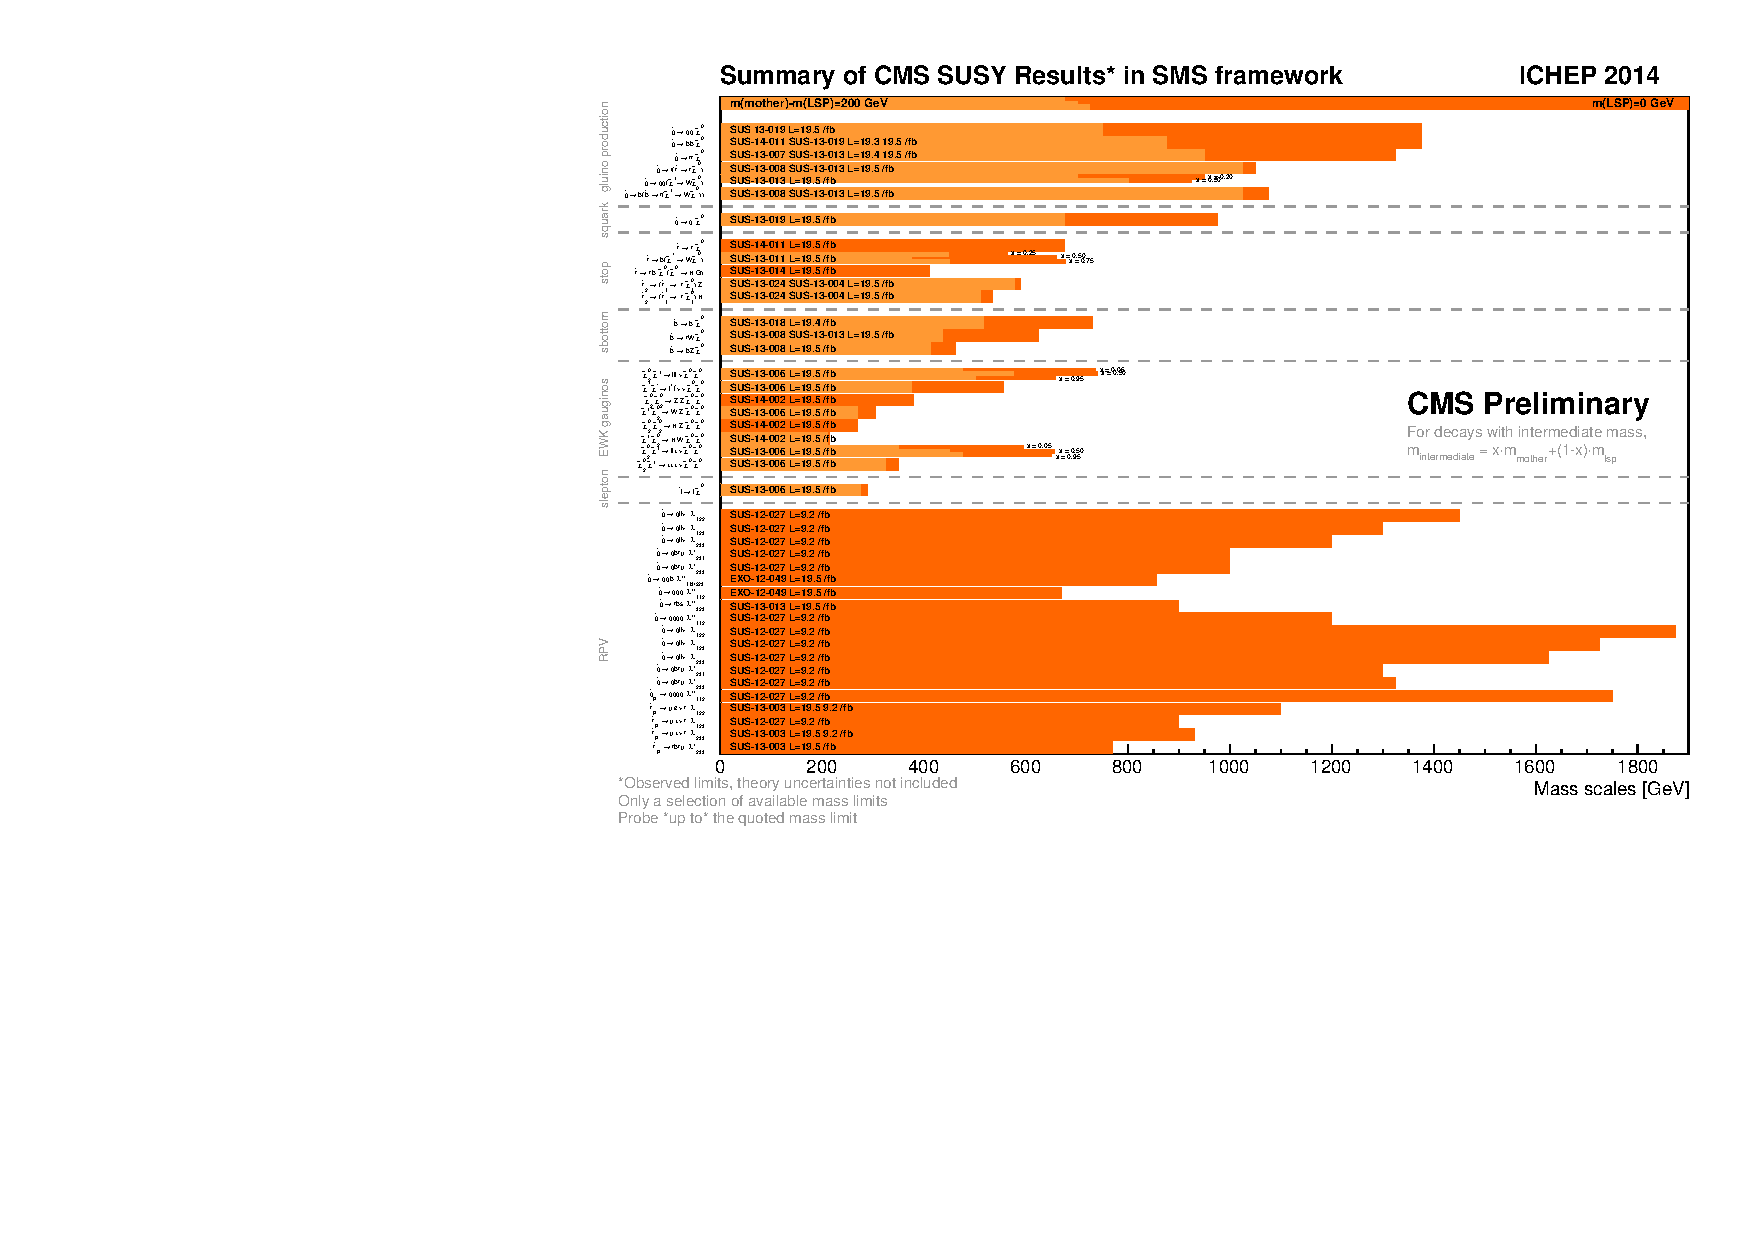
\includegraphics[height=350pt]{figures/barplot_ICHEP2014.pdf}
\caption{Summary of CMS exclusion limits for the masses of various SUSY particles with $\sqrt{s}=8\TeV$ \cite{CMS-SUSY-LIMITS}. These limits assume simplified models and unity branching fractions for the specified decays. Two scenarios are presented: the dark shades show $m(\text{LSP})=0$ and the light shades show $m(\text{mother})-m(\text{LSP})=0$.}
\label{fig:cms-susy-limits}
\end{center}
\end{figure}
\end{landscape}
}

The introduction of $R$-parity violating (RPV) terms in the SUSY Lagrangian is one way to evade these limits. If $R$-parity is violated, SUSY particles can decay to final states containing only SM particles, avoiding the characteristically large \met from the LSP, which is no longer stable. This generally eliminates the LSP as a dark matter candidate, making it a less popular option. However, RPV SUSY still solves the hierarchy problem and assists in grand unification. The possible RPV terms in the superpotential are \cite{Barbier}:
\begin{equation}
W_{\text{RPV}} = \frac{1}{2}\lambda_{ijk}\PL_{i}\PL_{j}\PE_{k}^{c} + \lambda_{ijk}^{\prime}\PL_{i}\PQ_{j}\PD_{k}^{c} + \frac{1}{2}\lambda_{ijk}^{\prime \prime}\PU_{i}^{c}\PD_{j}^{c}\PD_{k}^{c} + \mu_{i}\PL_{i}\Hone. \label{eq:WRPV}
\end{equation}
The different RPV coupling constants are denoted as $\lambda_{ijk}$, $\lambda^{\prime}_{ijk}$, $\lambda^{\prime \prime}_{ijk}$, and $\mu_{i}$, where $i$, $j$, and $k$ are generation indices. Figure \ref{fig:trilinear-RPV} shows the tree-level diagrams for the trilinear RPV couplings. As indicated by Fig. \ref{fig:trilinear-RPV} and the definition of $R$ in Eq. \eqref{eq:Rdef}, violating $R$ is equivalent to violating lepton number or baryon number. Scenarios which include all of the RPV couplings include large contributions to proton decay, due to the violation of both $B$ and $L$, and are therefore ruled out. Scenarios in which only a certain type of RPV coupling is allowed can still be viable.

\begin{figure}[hbt]
\begin{center}
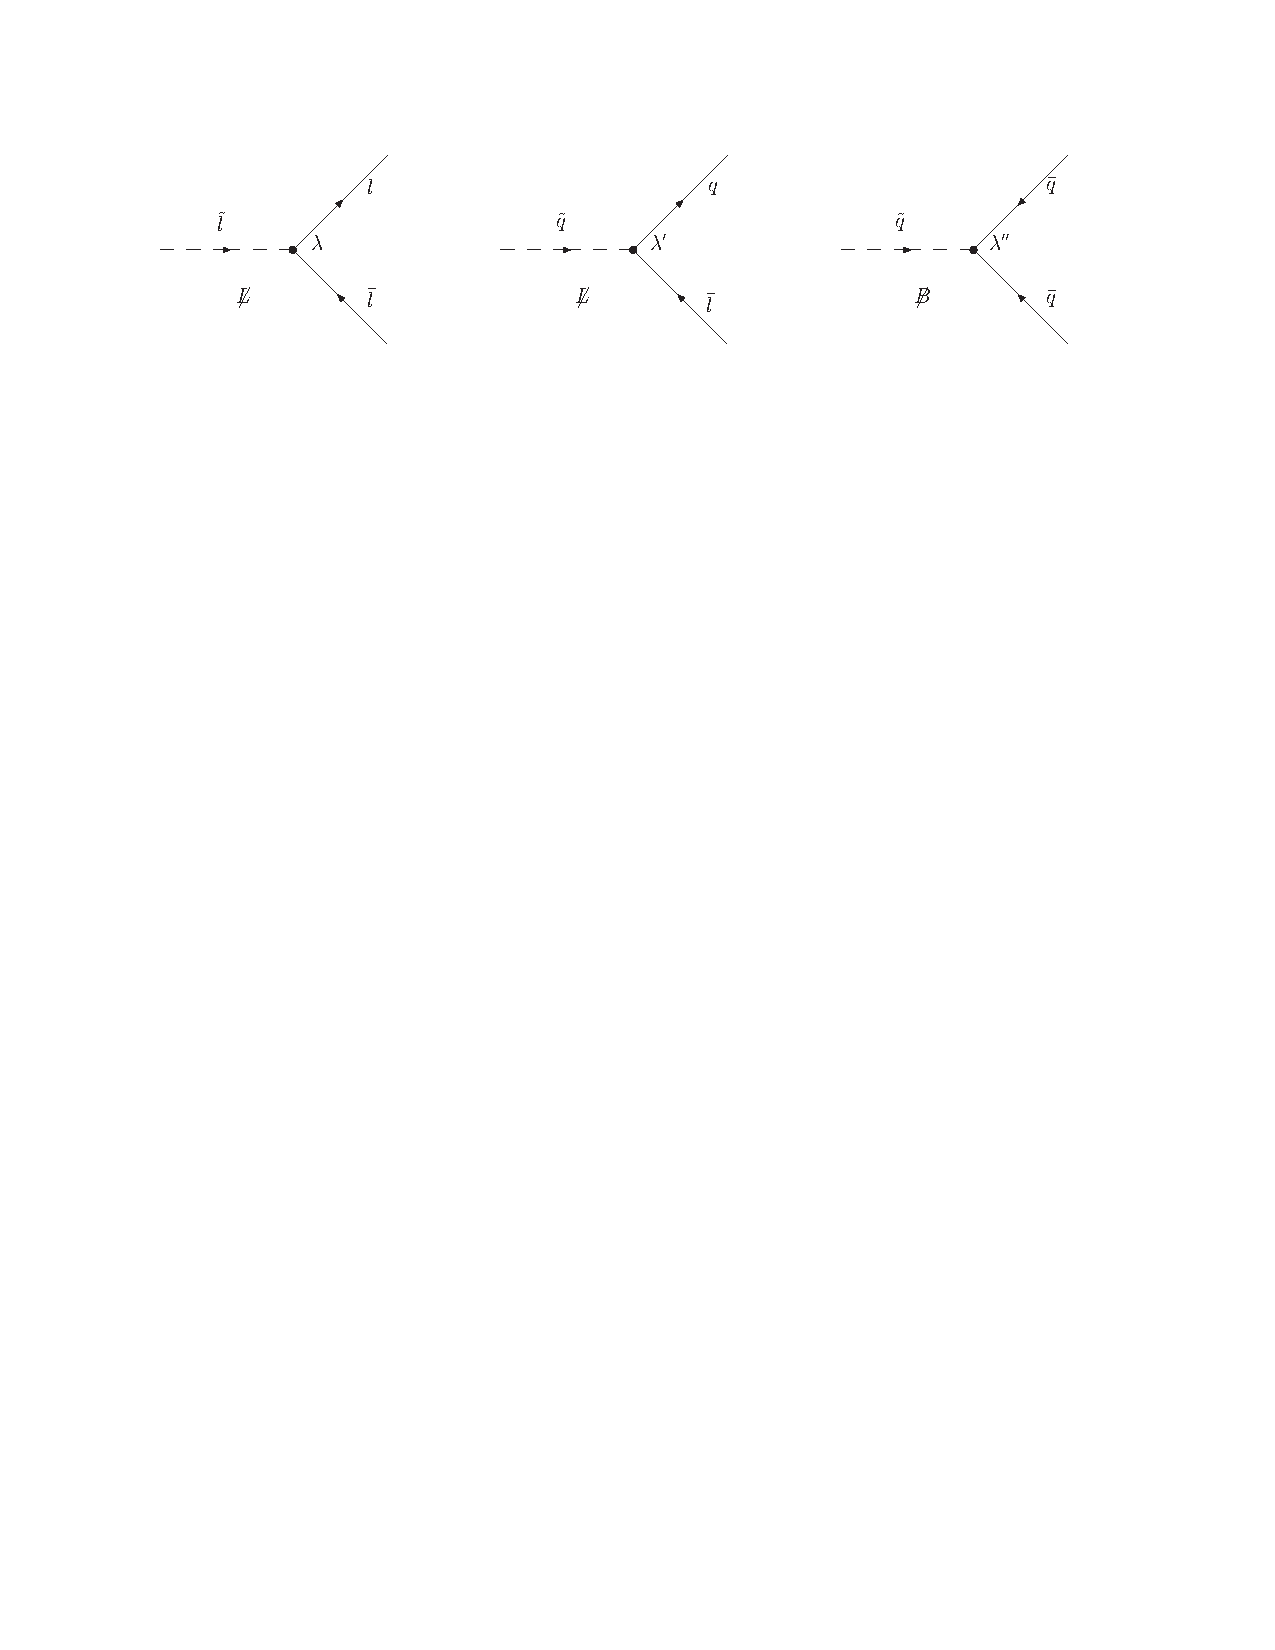
\includegraphics[width=0.95\textwidth]{figures/0406039v2_trilinear.pdf}
\caption{The LO diagrams for the three trilinear RPV couplings $\lambda$ (left), $\lambda^{\prime}$ (middle), and $\lambda^{\prime \prime}$ (right) \cite{Barbier}. These couplings violate lepton number, lepton number, and baryon number, respectively.}
\label{fig:trilinear-RPV}
\end{center}
\end{figure}

This dissertation considers the pair production of top squarks with two different RPV decays, using a decoupled model as described above. As a strongly-interacting scalar particle, the top squark production cross section is identical to the leptoquark production cross section at leading order. In decoupled models, the cross section depends on the squark mass scale and the top squark mixing angle only at higher order, and the corrections from these terms amount to less than 2\% \cite{StopCrossSec}. The first decay considered is $\sTop \rightarrow \tau \cPqb$ via the coupling $\lambda_{333}^{\prime}$. The final-state signature and kinematic distributions of this signal are identical to those from the pair production of third-generation scalar leptoquarks, as described in Sec. \ref{sec:LQ}. Therefore, the results of the leptoquark search can be directly reinterpreted to apply to the $\lambda_{333}^{\prime}$ decay of top squarks.

In some natural SUSY models, if the higgsinos are lighter than the top squark, or if the RPV couplings that allow direct decays to SM particles are sufficiently small, the top squark decay may preferentially proceed via superpartners \cite{Jared}. This motivates the second search in the dissertation, which focuses on a scenario in which the dominant RPC decay of the top squark is $\sTop \rightarrow \chipm\cPqb$. This requires the mass splitting between the top squark and the chargino to be less than the mass of the top quark, so it is chosen to be 100\GeV. The chargino is assumed to be a pure higgsino and to be nearly degenerate in mass with the neutralino, with a decay $\chipm \rightarrow \sNu\tau^{\pm} \rightarrow \cPq\cPq\tau^{\pm}$. The decay of the sneutrino occurs via the RPV coupling $\lambda_{3jk}^{\prime}$, where the cases $j, k = 1, 2$ are considered. Such a signal can only be probed by searches that do not require large \met, as chiral suppression prevents the other possible decay of the chargino, $\chipm\to\nu\sTau$, from contributing to scenarios involving the $\lambda_{3jk}^{\prime}$ coupling.

The final state from pair production of top squarks undergoing this chargino-mediated RPV decay contains two tau leptons, two b-jets, and at least four additional jets. The search for the signal with this final state is called the top squark search, to distinguish it from the similar but not identical final state in the leptoquark search. As in the leptoquark search, the analysis is divided into two channels \etau and \mutau based on the required leptonic decay of one of the tau leptons. The symbol $\mathcal{B}$ in the top squark search is used to represent the branching fraction for the decay $\sTop \rightarrow \chipm\cPqb, \chipm \rightarrow \sNu\tau^{\pm} \rightarrow \cPq\cPq\tau^{\pm}$.  This dissertation presents the first search for the chargino-mediated $\lambda_{3jk}^{\prime}$ decay of the top squark.

\renewcommand{\thesection}{\thechapter.\arabic{section}} % back to regular numbering
% input: [cmsexperiment.tex]
\chapter{Compact Muon Solenoid Experiment
\label{ch:cmsexperiment}}
\setcounter{section}{-1}

The Compact Muon Solenoid (CMS) experiment is one of two general-purpose detectors at the LHC. It is located about 100\unit{m} underground at Point 5 of the LHC ring, near Cessy, France. The detector is cylindrically shaped, with total length 22\unit{m}, diameter 15\unit{m}, and weight 14000\unit{tons}. Figure \ref{fig:cms-overall} shows the overall layout of the detector. The following sections describe the LHC, based on Ref. \cite{LHCmachine}, and the CMS subdetector systems, based on Ref. \cite{CMSJINST}.

\begin{figure}[hbt]
\begin{center}
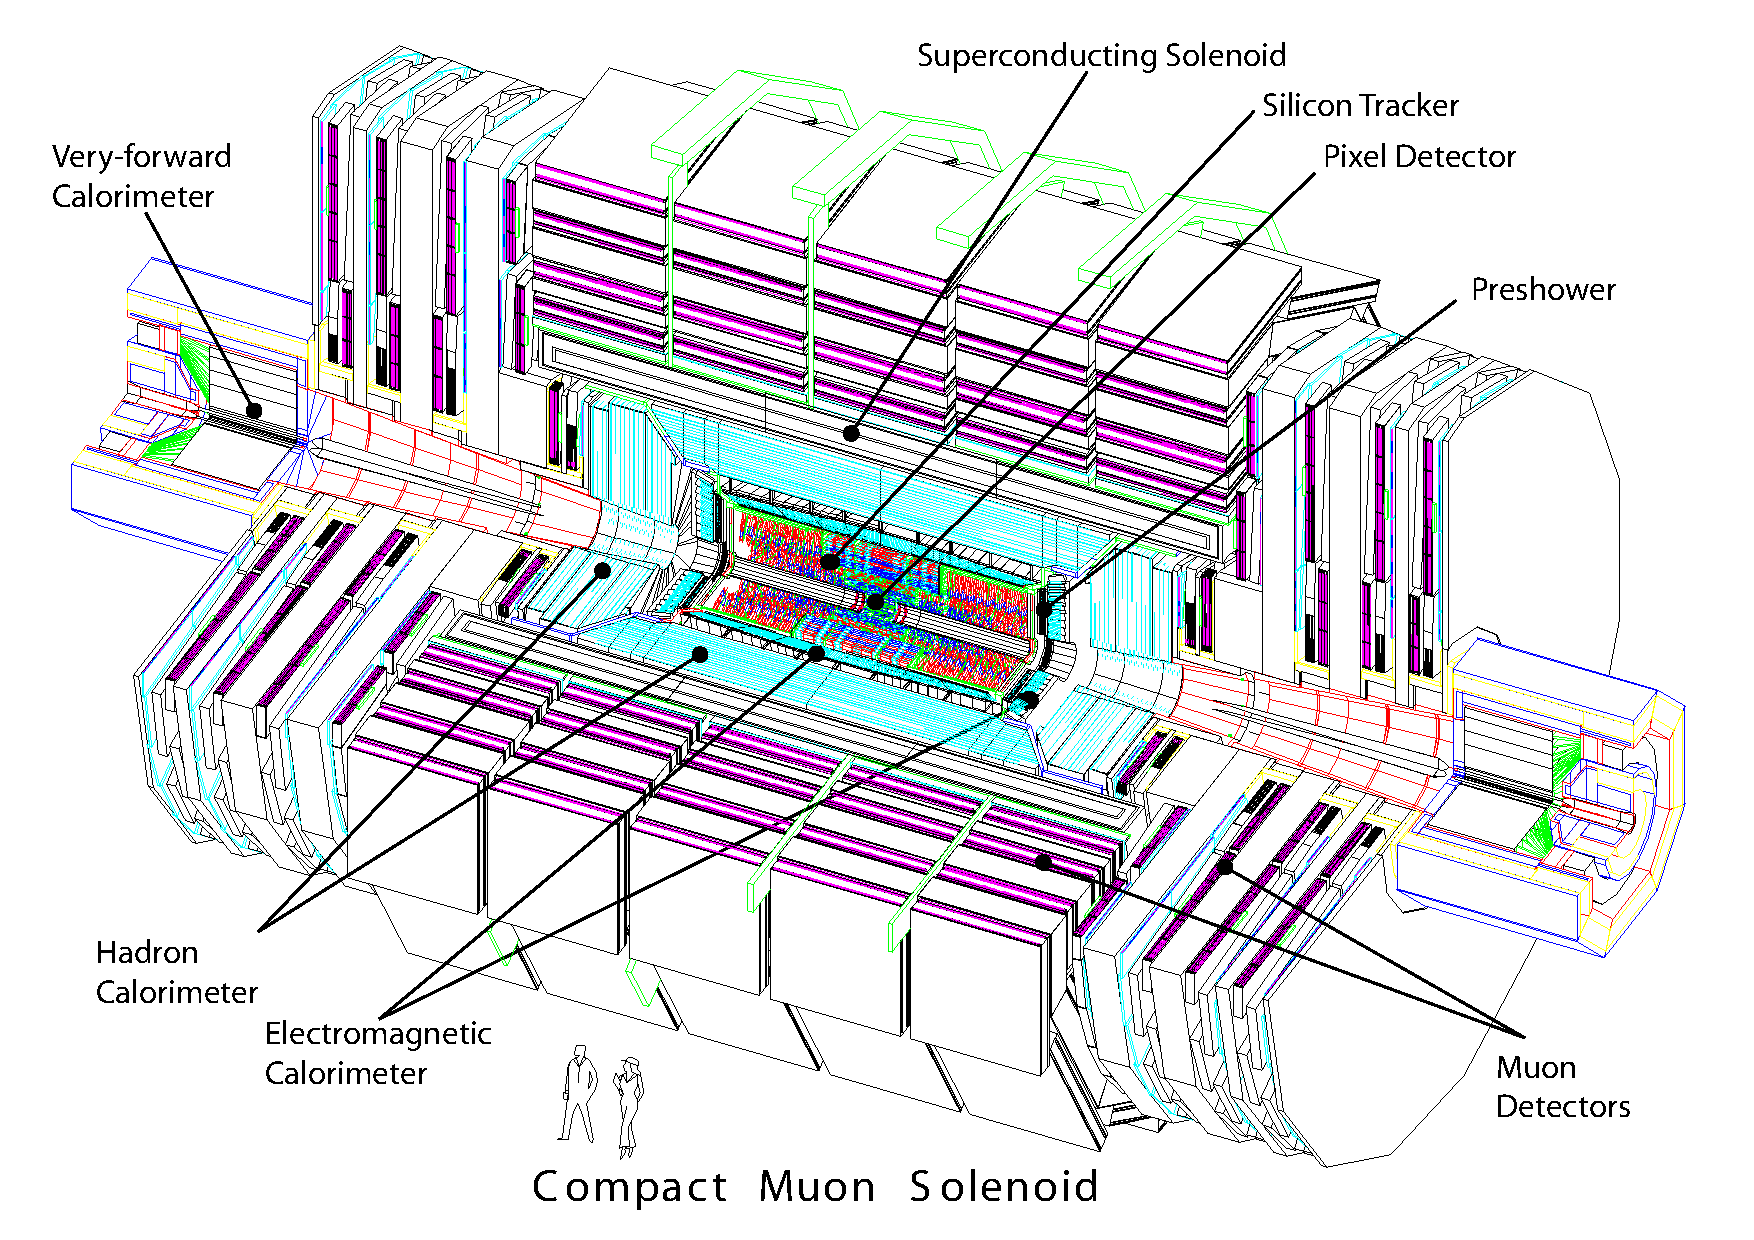
\includegraphics[width=0.95\textwidth]{figures/cms_complete_labelled.pdf}
\caption{The layout of the CMS detector, with the subdetectors labeled and two humans shown for a height reference.}
\label{fig:cms-overall}
\end{center}
\end{figure}

The center of the detector, the interaction point (IP), is used as the origin of the right-handed coordinate system that describes locations and directions within the detector. The $z$-axis is assigned to the direction of the LHC beam line. The polar angle $\theta$ is often transformed into pseudorapidity, defined as $\eta = -\text{ln}[\text{tan}(\theta/2)]$. Differences in pseudorapidity are Lorentz invariant for boosts in the $z$ direction, and particle production is approximately uniform in $\eta$. The plane transverse to the $z$-axis comprises the $x$- and $y$-axes, with the $x$-axis pointing toward the center of the LHC ring and the $y$-axis pointing upward in the normal direction. The azimuthal angle $\phi$ and the radial coordinate $r$ are also defined in the transverse plane. The magnitude of the component of momentum in the transverse plane is labeled \pt.

\section{The Large Hadron Collider}

The Large Hadron Collider is the largest machine ever built and the highest-energy collider in the world. It uses the tunnel originally constructed for the Large Electron-Positron Collider (LEP) with a circumference of 26.7\unit{km}. The tunnel is located underground in Switzerland and France, near Geneva. Figure \ref{fig:lhc-diagram} shows a diagram of the LHC. The location of the CMS experiment is provided and the other major experiments are also indicated.

\begin{figure}[hbt]
\begin{center}
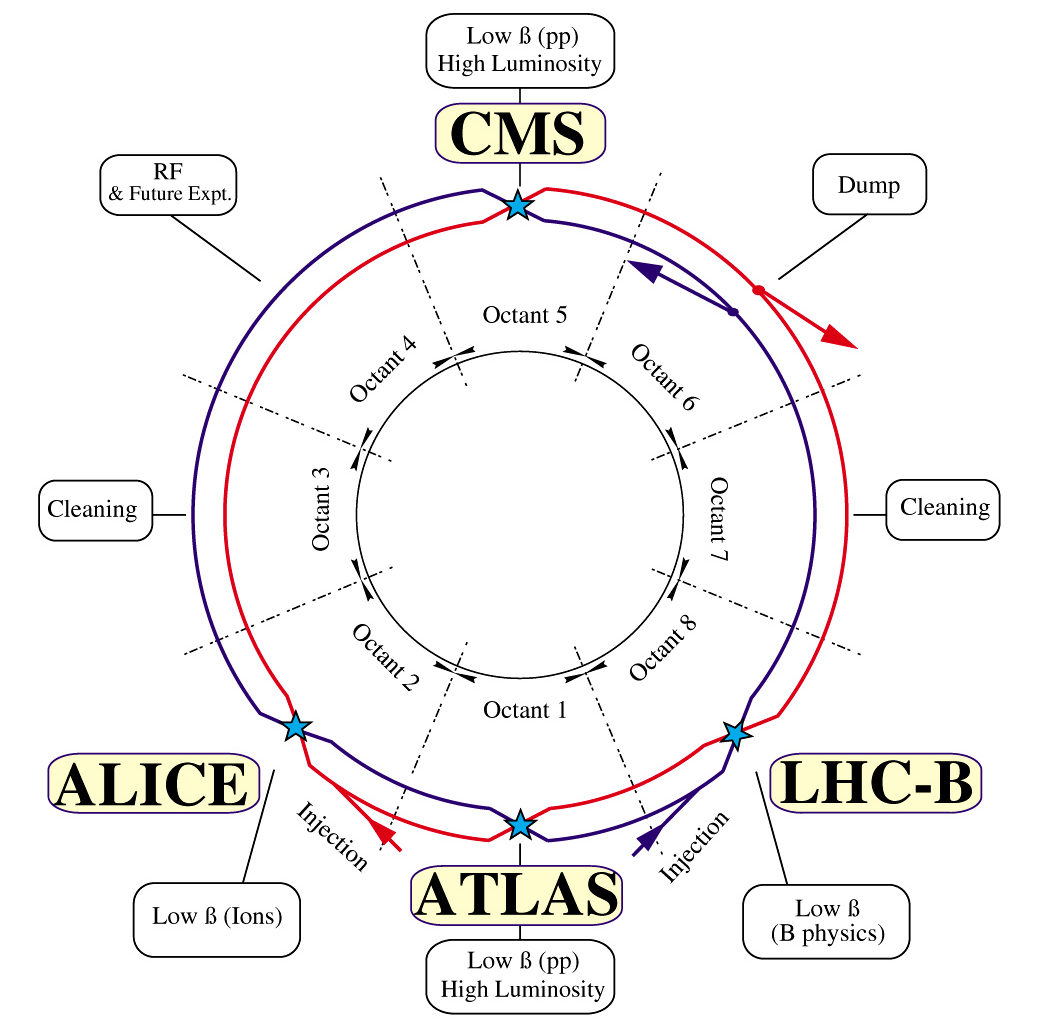
\includegraphics[width=0.95\textwidth]{figures/lhc-pho-1997-060.png}
\caption{A diagram of the LHC with the major experiments labeled \cite{Jean-Luc:841573}.}
\label{fig:lhc-diagram}
\end{center}
\end{figure}

The LHC is designed to accelerate two beams of protons up to energies of 7\TeV each, at instantaneous luminosities up to $10^{34}\percms$. The use of supercooled superconducting magnets, discussed below, is crucial. Several stages of CERN accelerators are used to inject proton beams into the LHC, as shown in Fig. \ref{fig:lhc-injectors}. These include the linear accelerator Linac2, the Proton Synchrotron Booster (PSB), the Proton Synchrotron (PS), and the Super Proton Synchrotron (SPS). The accelerated protons are grouped into bunches using radio frequency (RF) electromagnetic fields. The LHC is designed to accommodate a bunch spacing of 25\unit{ns}.

\begin{figure}[hbt]
\begin{center}
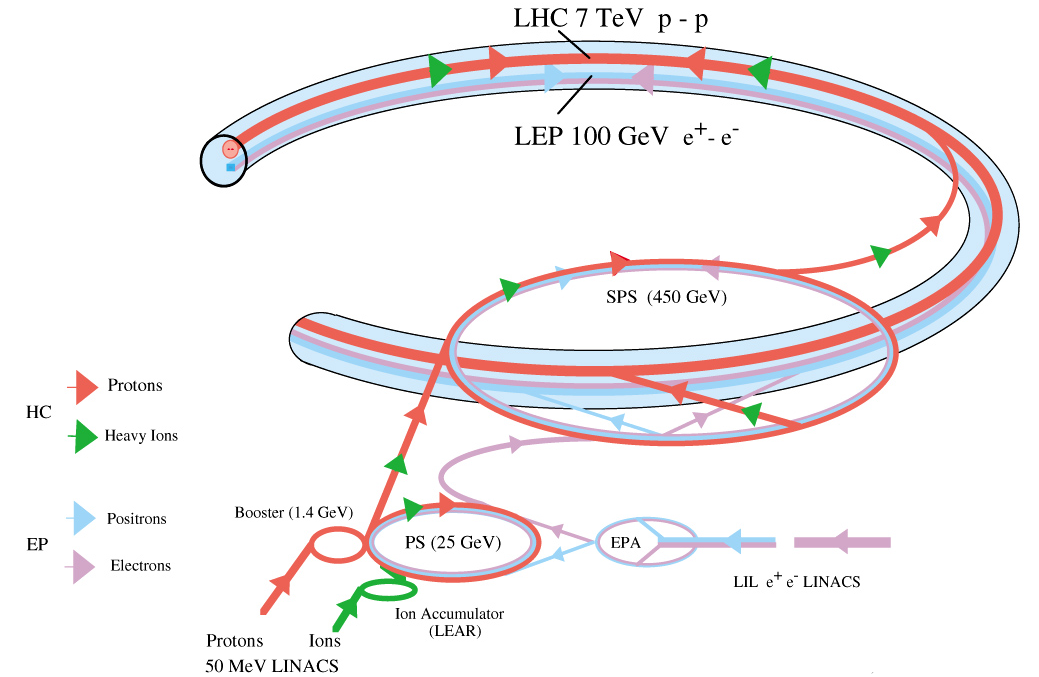
\includegraphics[width=0.95\textwidth]{figures/lhc-pho-1993-008.png}
\caption{A diagram of the CERN accelerators which form the LHC injector \cite{Jean-Luc:841568}.}
\label{fig:lhc-injectors}
\end{center}
\end{figure}

Due to size limitations in the tunnel, the two rings used to accelerate the two proton beams are formed by twin bore magnets. Each magnet has a single mechanical structure and cryostat, in which are placed two coils and two beam channels. The dipole magnet coils use superconducting NbTi Rutherford cables cooled to 1.9\unit{K}, as shown in Fig. \ref{fig:lhc-dipole}, with a design field strength of 8.33\unit{T} for acceleration of protons up to 7\TeV. This extreme cooling is accomplished using superfluid helium. In total, the LHC contains 1232 dipole magnets. Thousands of quadrupole, sextupole, octupole, and decapole magnets are used to correct and focus the beam.

\begin{figure}[hbt]
\begin{center}
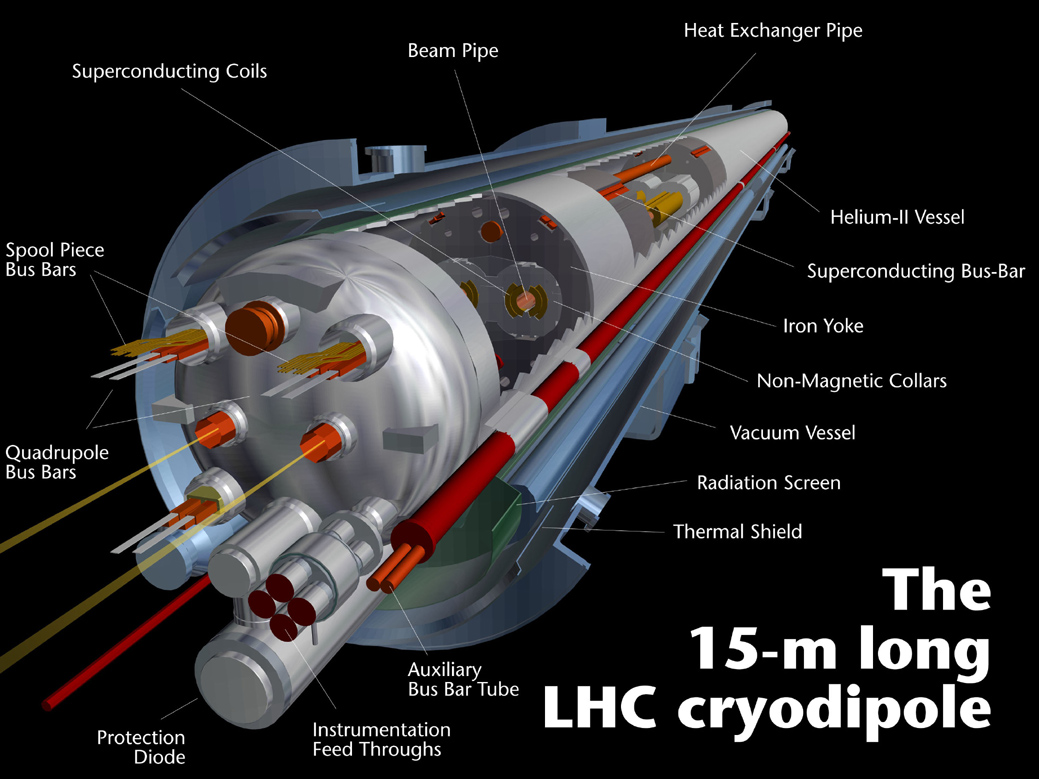
\includegraphics[width=0.95\textwidth]{figures/lhc-pho-1998-299.jpg}
\caption{A diagram of an LHC dipole magnet, with the major components labeled \cite{Dailler:842253}.}
\label{fig:lhc-dipole}
\end{center}
\end{figure}

In 2012, the LHC accelerated proton beams to energies of 4\TeV each, with a peak instantaneous luminosity of $7.67\times10^{33}\percms$ and a bunch spacing of 50\unit{ns}. During that year, it delivered 23.30\fbinv of integrated luminosity to the CMS detector, of which 21.79\fbinv was recorded \cite{LumiPublic}. In the upcoming 2015 run, the LHC will achieve its design energy, instantaneous luminosity, and bunch spacing.

\section{Tracker}
\label{sec:tracker}

The CMS tracker is the first subdetector to measure charged particles produced in collisions at the IP. It is 5.8\unit{m} long and 2.5\unit{m} in diameter, covering the pseudorapidity range $-2.5 < \eta < 2.5$. Two subsystems make up the tracker: the pixel detector and the silicon strip tracker. The layout of the tracker, with these subsystems labeled, is shown in Fig. \ref{fig:tk-layout}. Due to the tracker's location close to the IP, it experiences severe radiation doses that are expected to range from 0.18 to 84\unit{Mrad} after 500\fbinv of data. Hence, the tracker must be robust against radiation damage, requiring operation at $-10\degC$ and influencing the design of the sensors and electronics. For tracks with momentum of 100\GeV, the tracker has a transverse momentum resolution of 1--2\% for $|\eta|<1.6$; at higher $\eta$, the reduced transverse depth of the tracker degrades the resolution.

\begin{figure}[hbt]
\begin{center}
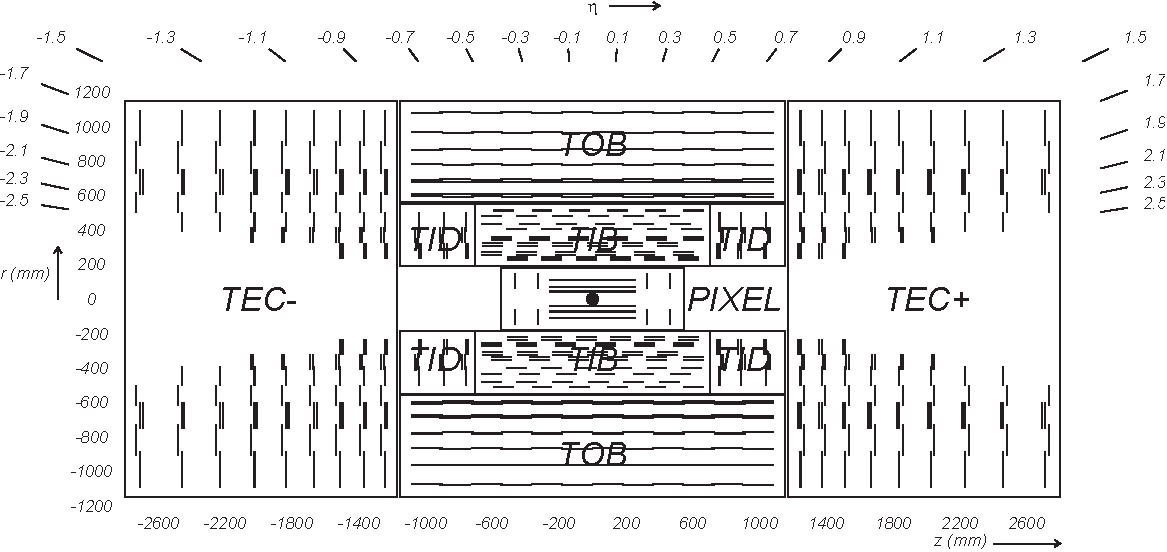
\includegraphics[width=0.95\textwidth]{figures/CMS_tracker.pdf}
\caption{The layout of the CMS tracker, with subsystems labeled.}
\label{fig:tk-layout}
\end{center}
\end{figure}

The pixel detector is the innermost portion of the tracker. It consists of three barrel layers, collectively called BPIX, and two endcap layers, called FPIX. Each pixel cell is a hybrid silicon detector with dimensions $100\times150\mum^{2}$. The small pixel size enables precise track resolutions of 10\mum in the $r$-$\phi$ direction and 20\mum in the $z$ direction. In total, the BPIX comprises 48 million pixels and the FPIX comprises 18 million pixels. The pixel detector is important for many key components of CMS physics analysis. These include the reconstruction of secondary vertices from decays of tau leptons and bottom quarks, as well as producing seed tracks for the strip tracker and the high level trigger.

The silicon strip detector consists of four subsystems. The Tracker Inner Barrel (TIB) has four layers with the three-layer Tracker Inner Disks (TID) at each end; both systems' strips are 320\mum thick. Surrounding the TIB/TID is the Tracker Outer Barrel (TOB), which has six layers. The first four layers of the TOB use 500\mum thick strips, while the last two layers use 122\mum thick strips. The Tracker EndCaps (TEC) have nine disks with up to seven layers of strips, 320\mum thick in the inner four rings and 500\mum thick in the outer three rings. In total, all of these layers contain 9.3 million silicon strips.

The tracker maintained excellent performance during the 2012 run of the LHC. The pixel detector had 97.7\% of channels operational in BPIX and 92.8\% of channels operational in FPIX, while 97.5\% of channels in the strip detector were active. The hit reconstruction efficiencies were greater than 99\% for each layer of the strip detector and greater than 99.5\% for each layer of the pixel except for the first layer of BPIX, which had an efficiency greater than 99.2\% \cite{Veszpremi:2014hpa}. 

\section{Electromagnetic Calorimeter}

The electromagnetic calorimeter (ECAL) is a homogeneous calorimeter constructed entirely of lead tungstate (\pbwo) crystals. The ECAL is divided into two subsystems: the ECAL barrel (EB) and the ECAL endcap (EE). In the endcap region, there is an additional ECAL preshower (ES) detector in front of the EE. Figure \ref{fig:ecal-layout} displays these subsystems. \pbwo has a peak emission wavelength of 425\unit{nm} and many desirable material properties. These properties include high density ($8.28\unit{g/cm}^3$), short radiation length (0.89\cm), short Moli\`{e}re radius (2.2\cm), and fast decay time (6\unit{ns}). The use of homogeneous \pbwo crystals enables precise energy resolution for electromagnetic objects. For photons with $\ET \approx 60\GeV$, the energy resolution ranges from 1.1\% to 2.6\% for the EB and 2.2\% to 5.0\% for the EE. In general, the energy resolution $\sigma$ varies as a function of energy $E$ in \GeVns:
\begin{equation}
\label{eq:ecal-res} \left(\frac{\sigma}{E}\right)^{2} = \left(\frac{S}{\sqrt{E}}\right)^{2} + \left(\frac{N}{E}\right)^{2} + C^{2}.
\end{equation}
In Eq. \eqref{eq:ecal-res}, $S$ is the stochastic term, $N$ is the noise term, and $C$ is the constant term. Typical values for these terms were measured by a test beam to be $S=2.8\%$, $N=12\%$, $C=0.30\%$.

\begin{figure}[hbt]
\begin{center}
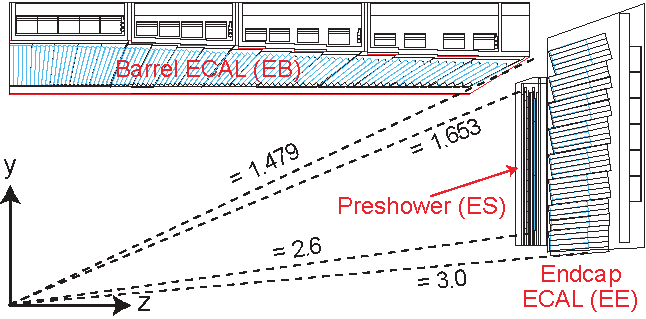
\includegraphics[width=0.95\textwidth]{figures/ECAL_transverse_section.pdf}
\caption{A diagram of the CMS ECAL, with subsystems and $\eta$ ranges labeled.}
\label{fig:ecal-layout}
\end{center}
\end{figure}

The EB contains 61200 \pbwo crystals and covers the range $|\eta|<1.479$. The crystals are arranged in a projective geometry with a tapered shape. The crystal granularity is approximately $0.0174\times0.0174$ in $\eta$-$\phi$, corresponding to dimensions of $22\times22\mm^{2}$ at the front face and $26\times26\mm^{2}$ at the back face. The EB has a depth of 230\mm or 25.8 radiation lengths ($X_{0}$). The scintillation light produced by the \pbwo crystals is read out using avalanche photodiodes (APDs). At 18\degC, the APDs measure approximately 4.5 photoelectrons per \MeVns. The dark current of the APDs is sensitive to radiation exposure. Over the course of the 2012 run, the dark current ranged from 0.3--1.3\muA on average, corresponding to an average noise of 47--57\MeV \cite{CMS:2013ecal}.

The EE contains 14648 \pbwo crystals and covers the range $1.479<|\eta|<3.0$. The crystals are arranged in a non-projective $x$-$y$ geometry, with dimensions of $28.62\times28.62\mm^{2}$ at the front face and $30\times30\mm^{2}$ at the back face. The EE has a depth of 220\mm or 24.7$\,X_{0}$. Vacuum phototriodes (VPTs) are used as the photodetectors to read out the scintillation light from the \pbwo crystals. They collect approximately 4.5 photoelectrons per \MeVns at 18\degC. During the 2012 run, the average noise ranged from 180--220\MeV, with a more dramatic increase up to 600\MeV at high $\eta$ because of the high radiation dose \cite{CMS:2013ecal}.

The ES is intended to identify neutral pions in the endcap region, covering the range $1.653<|\eta|<2.6$. It is a sampling calorimeter with two layers of lead absorber and silicon strip detectors. The first layer of lead absorber has a thickness of 2$\,X_{0}$, while the second layer has a thickness of 1$\,X_{0}$. Each layer of silicon strips is 320\mum thick and can collect 3.6\unit{fC} of charge from a minimum ionizing particle.

%add percentage of live channels for EB and EE in 2012 run? and HE raddam?

\section{Hadron Calorimeter}

The hadron calorimeter (HCAL) is a sampling calorimeter which measures the energy of hadronic particles. The HCAL is especially important for measuring neutral hadrons, which do not leave tracks in the tracker. In addition, by containing all hadronic activity in each event within $|n|<5$, the HCAL enables the measurement of \met caused by neutrinos and other theoretical weakly-interacting particles. The HCAL consists of four subsystems. Three of these subsystems use similar technology: the HCAL barrel (HB), the HCAL endcap (HE), and the HCAL outer (HO). The fourth subsystem, the HCAL forward (HF), uses an alternative technology necessary to survive the high radiation doses at its forward location. The locations of the various HCAL subsystems in the CMS detector are shown in Fig. \ref{fig:hcal-layout}. The calorimeter system, combining the ECAL and the HCAL, can measure jets with a resolution $\sigma/E \approx 100\% / \sqrt{E\,[\GeVns]} \oplus 5\%$ that varies with the jet energy $E$.

\begin{figure}[hbt]
\begin{center}
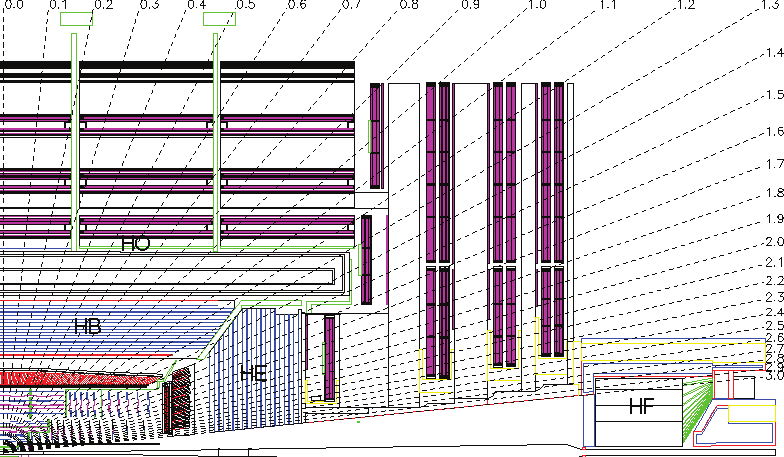
\includegraphics[width=0.95\textwidth]{figures/HCAL_subdet.pdf}
\caption{The layout of the HCAL subsystems HB, HE, HO, and HF in the CMS detector.}
\label{fig:hcal-layout}
\end{center}
\end{figure}

The HB is a 16-layer sampling calorimeter covering the range $|\eta|<1.3$. The absorbing layers are made of C26000 cartridge brass, composed of 70\% copper and 30\% zinc. Cartridge brass has a density of $8.53\unit{g/cm}^3$, a radiation length of 1.49\cm, and a nuclear interaction length of 16.42\cm. The first absorbing layer in the HB is a 40-mm-thick steel plate. The next eight absorbing layers are 50.5-mm-thick brass plates, and the subsequent six absorbing layers are 56.5-mm-thick brass plates. The last absorbing layer is a 75-mm-thick steel plate. The overall thickness of the HB absorber ranges from 5.82$\,\lambda_{0}$ at $\eta=0$ to 10.6$\,\lambda_{0}$ at $|\eta|=1.3$. The EB in front of the HB has a thickness of 1.1$\,\lambda_{0}$ and can measure the electromagnetic portions of early developing hadronic showers. The scintillating layers consist of 3.7-mm-thick Kuraray SCSN81 plastic scintillator, a polystyrene base doped with fluors. The exception is Layer 16, which has a thickness of 9\mm, in order to sample more from late developing hadronic showers. At the front of the HB, before the first absorbing layer, is the scintillator Layer 0, which is 9\mm of Bicron BC408 plastic scintillator, a polyvinyltoluene base doped with fluors. Layer 0 samples the energy deposited by hadronic showers in the dead material between the EB and the HB. The scintillator tiles are arranged in a projective geometry with a granularity of $0.087\times0.087$ in $\eta$-$\phi$. In total, the HB has 16 $\eta$ divisions called towers, 36 $\phi$ divisions, and approximately 70000 tiles. The light from the scintillators is collected by Kuraray Y-11 green wavelength shifting (WLS) fiber, which is placed in a $\sigma$-shaped groove in the scintillator tiles. The wavelength-shifted light from multiple layers is brought together and read out by hybrid photodiodes (HPDs). These photodetectors were chosen because of their large dynamical range and low sensitivity to magnetic fields.

The thinness of the HB at low $\eta$ prevents it from fully containing hadronic showers, so the HO is added to act as an extension of the calorimeter system. The HO uses the same scintillator tile technology as the HB: 3.7-mm-thick SCSN81 with Y-11 WLS fiber and granularity $0.087\times0.087$ in $\eta$-$\phi$, read out by HPDs. The HO is divided into five rings, each with a width of 2.536\unit{m} in the $z$ direction, based on the structure of the iron return yoke outside of the solenoid. In the central Ring 0, the HO has two scintillating layers, one inside the solenoid and one outside of it. In the other rings, the HO has one scintillating layer outside of the solenoid. The thickness of the absorbing iron layer formed by the solenoid is 19.5\cm, extending the total depth of the calorimeter system to a minimum of 11.8$\,\lambda_{0}$.

The HE is a 17-layer sampling calorimeter covering the range $1.3<|\eta|<3.0$. Each absorbing layer consists of 79-mm-thick cartridge brass, the same material used for the HB absorbing layers. The scintillating layers use the same technology as the HB and the HO. In total, the HE contains 20916 scintillator tiles. The granularity of the tiles is the same as HB for $|eta|<1.6$; for higher $\eta$, they become coarser at approximately $0.17\times0.17$ in $\eta$-$\phi$. Unlike the HB, the scintillating layers in each tower are split into multiple groups called depths before being read out by HPDs. A diagram of the depth segmentation scheme is shown in Fig. \ref{fig:hcal-depths}. This depth segmentation allows for more precise recalibration of the HE, which experiences a higher radiation dose than the HB. Towers 27, 28, and 29, which are the closest to the beamline, have three readout depths, while the other towers have two readout depths. The crossover region between the HB and the HE, towers 15 and 16, also utilize depth segmentation. As in the HB, Layer 0 in the HE consists of 9-mm-thick BC408 to sample from the dead material between the EE and the HE. The combined calorimeter system, including both the EE and the HE, has an approximate thickness of 10$\,\lambda_{0}$.

The HF covers the range $3.0<|\eta|<5.0$, with no ECAL in front of it. It consists of a steel absorber structure with a thickness of 165\cm or 10$\,\lambda_{0}$. Polymer-cladded quartz fibers with diameter 800\mum are embedded in the steel absorber. The fibers are bundled together to form 13 towers in a non-projective $x$-$y$ geometry with granularity $0.175\times0.175$ in $\eta$-$\phi$. Over 1000\unit{km} of fiber is used in the HF. Half of the fibers run for the full 165\cm depth of the detector, while the other half start 22\cm into the detector. Each type of fiber is read out separately in order to distinguish electromagnetic showers from hadronic showers. The fibers measure particle showers using Cherenkov light, which is read out by photomultiplier tubes (PMTs). They measure approximately 1 photoelectron for every 4\GeV of energy deposited. This alternative design was necessary to ensure the radiation hardness of the HF, parts of which can experience 100\unit{Mrad/year}.

\begin{figure}[hbt]
\begin{center}
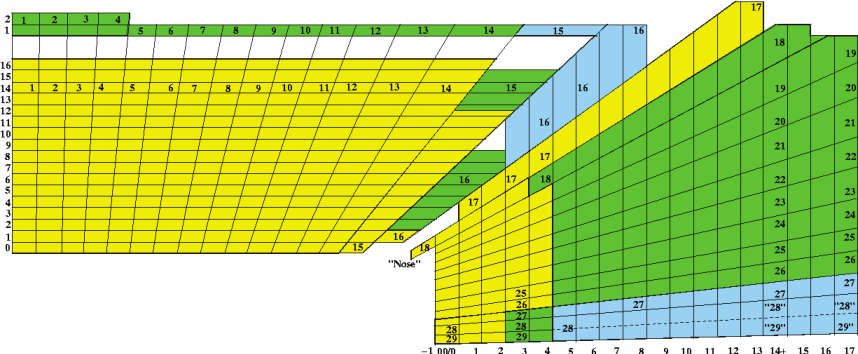
\includegraphics[width=0.95\textwidth]{figures/HCAL_tower_segmentation.pdf}
\caption{A diagram of the depth segmentation scheme in the HB and the HE.}
\label{fig:hcal-depths}
\end{center}
\end{figure}

%add percentage of live channels for HCAL in 2012 run?

\section{Solenoid}

The superconducting solenoid is the central feature of the CMS detector. The solenoid provides a magnetic field of 3.8\unit{T} within the volume formed by its diameter of 6\unit{m} and length of 12.5\unit{m}. This strong magnet field is necessary so that high energy charged particles bend sufficiently for the tracker to measure their momenta accurately. At full current, the solenoid has a stored energy of 2.35\unit{GJ}. The magnet is constructed from a 4-layer winding of reinforced NbTi conductor, cooled to 4.5\unit{K}. It is split into five rings of equal length. The cold mass of the magnet is 220 tons, and the high ratio between the stored energy and the cold mass, 11.6\unit{KJ/kg}, causes a significant mechanical deformation of 0.15\% when the magnet is powered. Figure \ref{fig:solenoid} shows an artistic rendering of the solenoid.

\begin{figure}[hbt]
\begin{center}
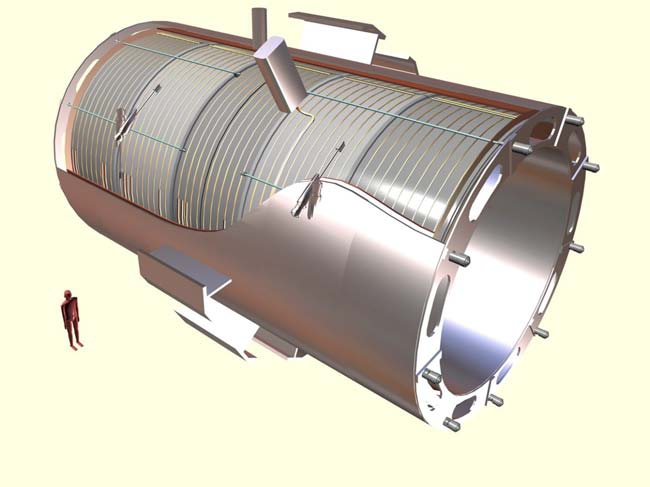
\includegraphics[width=0.95\textwidth]{figures/CMS_solenoid.jpg}
\caption{An artistic rendering of the CMS solenoid, showing the five rings placed inside the cryostat, along with the support structure.}
\label{fig:solenoid}
\end{center}
\end{figure}

\section{Muon System}
\label{sec:muon-system}

The identification and measurement of muons is a major focus of the CMS experiment. The CMS muon system comprises three subsystems, each utilizing different gaseous particle detection technology. In the barrel region, drift tubes (DTs) are used. In the endcap region, cathode strip chambers (CSCs) are used. Resistive plate chambers (RPCs) are also used in both regions. The muon systems are built into the iron yoke, which consists of five barrel rings and six endcap disks weighing 10000 tons in total. The yoke confines the outer magnetic field from the return flux from the solenoid and absorbs stray hadrons. The layout of the muon system is shown in Fig. \ref{fig:muon-system}. The momentum resolution of the muon system by itself is approximately 9\% for $\pt<200\GeV$ with low $\eta$ and low $p$. For 1\TeV muons, the resolution varies between 15\% and 40\%, depending on $|\eta|$. When the muon system measurements are combined with measurements from the tracker, the 1\TeV muon resolution is improved to 5\%.

\begin{figure}[hbt]
\begin{center}
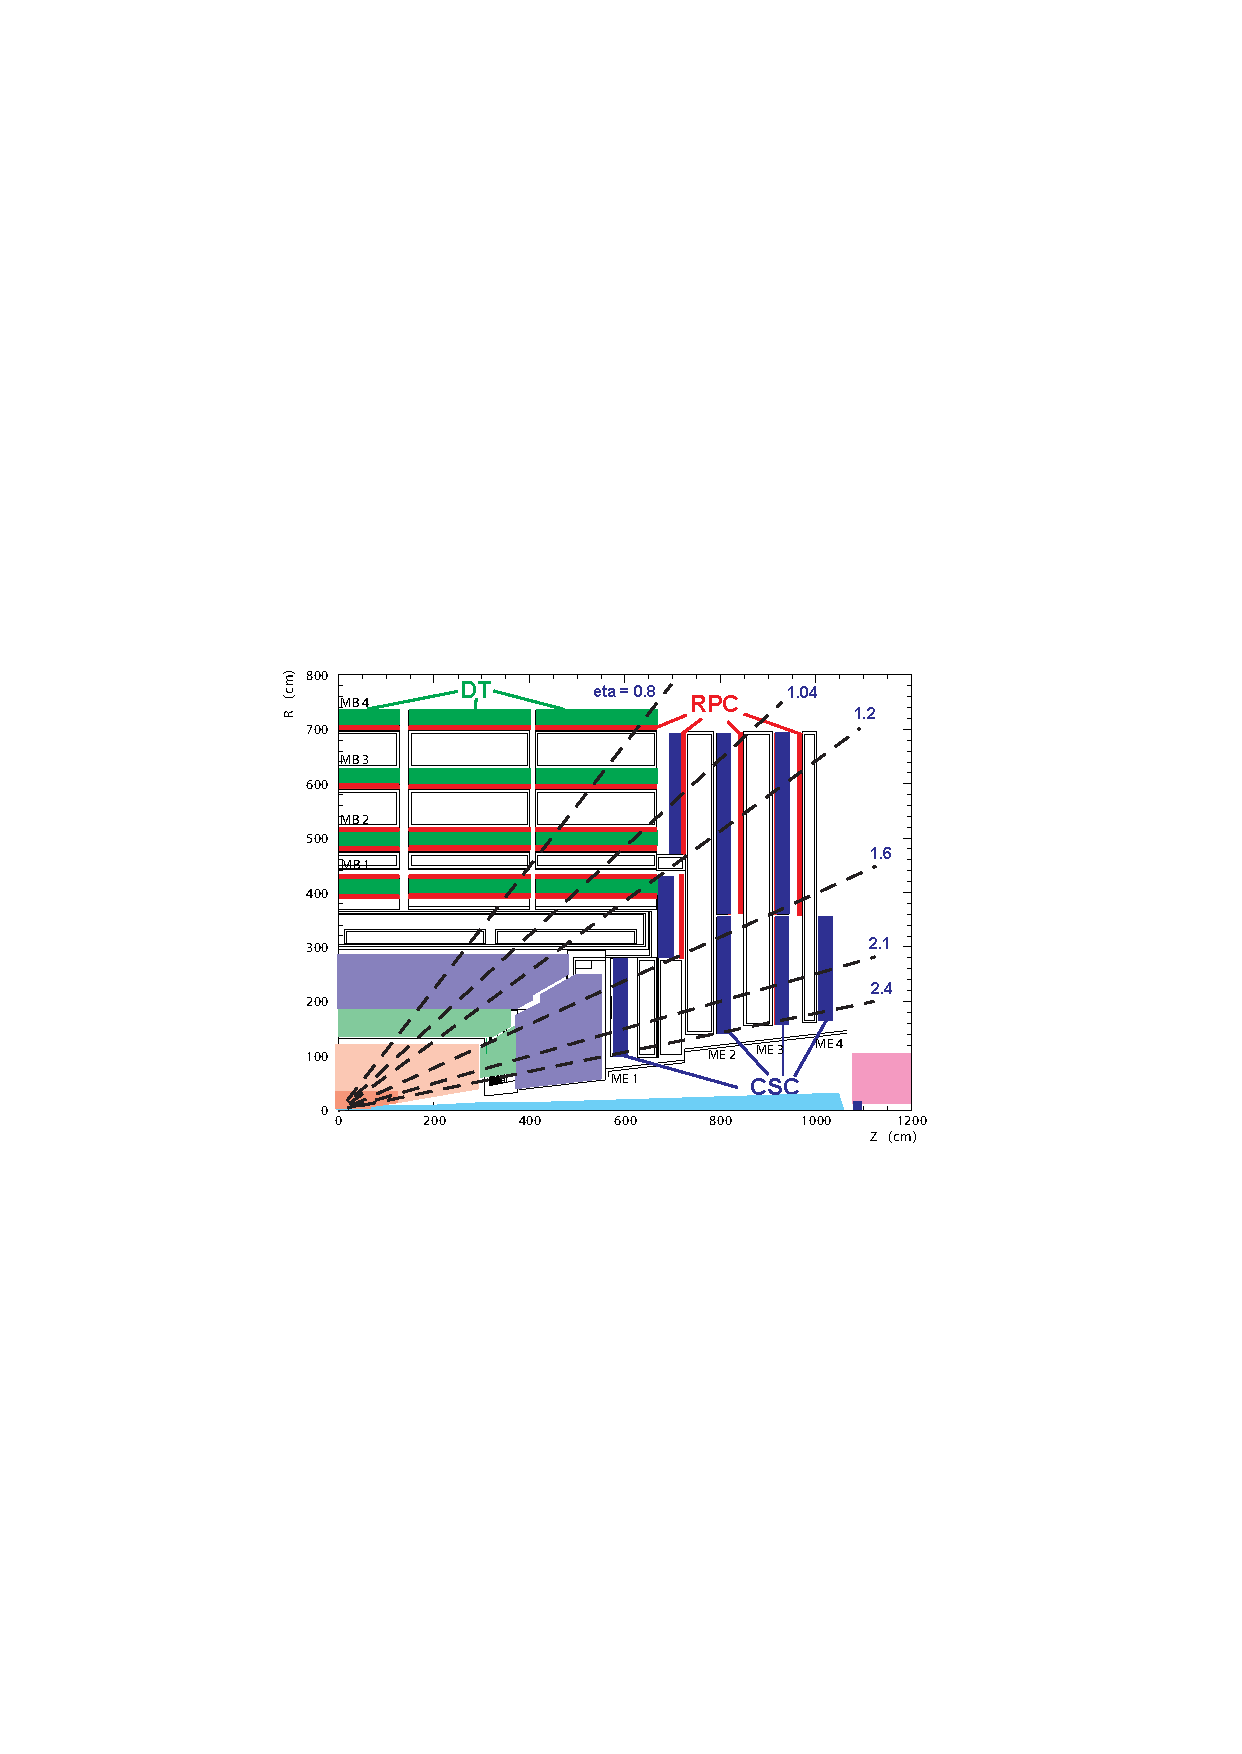
\includegraphics[width=0.95\textwidth]{figures/CMS_muon_system.pdf}
\caption{The layout of the muon system, with the three subsystems labeled.}
\label{fig:muon-system}
\end{center}
\end{figure}

The DTs are divided into four stations, which together cover the range $|\eta|<1.2$ and are labeled MB1 through MB4 (Muon Barrel). The first three stations each contain twelve chambers divided into three groups of four. Two of the groups of four measure the $r$-$\phi$ coordinate of muons, while the third group of four measures the $z$ coordinate. MB4 does not include a group of chambers that measures $z$. All four stations together contain 250 DTs with a total of 172000 sensitive wires. The gas used in the DTs is a mixture of 85\% Ar and 15\% $\text{CO}_2$, and the anode wires are gold-plated stainless steel with a diameter of 50\mum. Within $|\eta|<0.8$, the MB stations alone can reconstruct high-\pt muon tracks with an efficiency exceeding 95\%. The global $r$-$\phi$ resolution is 100\mum.

The CSCs are also divided into four stations and cover the range $0.9<|\eta|<2.4$. The four stations are labeled ME1 through ME4 (Muon Endcap). Each station is divided into several groups as follows: ME1 has three groups of 72 CSCs; ME2 and ME3 each have one group of 36 CSCs and another group of 72 CSCs; ME4 has one group of 36 CSCs. The total number of CSCs is thus 468. The cathode strips are arranged in the radial direction to measure the $r$-$\phi$ coordinate, while the anode wires are perpendicular to the strips to measure $\eta$. There are approximately 220000 cathode strip readout channels and 180000 anode wire readout channels. The CSC gas mixture is set at 40\% AR, 50\% $\text{CO}_2$, and 10\% $\text{CF}_4$. The cathode strips are formed from a fiberglass/epoxy material called FR4, coated with 36-$\mu$m-thick copper. The anode wires are made of gold-plated tungsten with a diameter of 50\mum. The first group of ME1 CSCs uses slightly thinner wire with 30\mum diameter and has some other slightly modified properties.

To complement the DTs and CSCs, RPCs are installed in both the barrel and endcap regions, covering the range $|\eta|<1.6$. The RPCs are primarily used to provide muon trigger information, due to fast tagging capabilities which allow them to precisely identify the bunch crossing time of muon candidate events. MB1 and MB2 each have one internal and one external group of RPCs, relative to the DTs; MB3 and MB4 each have two internal groups of RPCs. These groups together comprise 480 chambers. In the endcap, there are three RPC stations mounted in concentric circles on the iron yoke disks, with a total of 144 chambers. The RPCs are parallel plate detectors filled with a gas mixture of 96.2\% $\text{C}_2\text{H}_2\text{F}_4$, 3.5\% $i\text{C}_4\text{H}_{10}$, and 0.3\% $\text{SF}_6$.

%add percentage of live channels for muon system in 2012 run?

\section{Trigger}

The LHC operates at a high instantaneous luminosity, up to $10^{34}\percms$. With an expected proton-proton cross section of 100\unit{mb} at the LHC center-of-mass energies, the collision rate is approximately 1\unit{MHz}. The CMS trigger is necessary to reduce this high rate of collision events to a rate which can be stored and processed. The trigger system consists of two stages. The first stage uses hardware and is called the Level-1 (L1) Trigger. The L1 Trigger is designed to have a maximum output rate of 100\unit{kHz}. The second stage is the High Level Trigger (HLT), which uses software and reduces the output rate to $\mathcal{O}(100\unit{Hz})$.

The L1 Trigger uses custom-built programmable electronics, including field-programmable gate arrays (FPGAs), memory lookup tables (LUTs), and application-specific integrated circuits (ASICs). All of the subdetectors send input to the L1 Trigger, which is organized into local, regional, and global components as shown in Fig. \ref{fig:L1-trigger}. The local components, Trigger Primitive Generators (TPGs), are constructed from energy deposits in the calorimeters and track segments or hit patters from the muon system.

The TPGs from the ECAL, the HCAL, and the HF are combined into the Regional Calorimeter Trigger (RCT). The RCT groups calorimeter trigger towers into regions, which are made up of four towers in the barrel and endcap, and one tower in the HF. These regions are used to determine electron and photon candidates, as well as transverse energy sums (\sumet) and tau-jet vetoes. The RCT also passes MIP and isolation information to the muon triggers. Using information from the RCT, the Global Calorimeter Trigger (GCT) determines jet candidates and counts, providing up to four jets and four tau-jets from the central HCAL and four jets from the HF. The GCT also determines total \ET, \met, and \HT, which is calculated as \sumet for all jets above a certain threshold.

In parallel, the muon DT, CSC, and RPC systems each produce their own local triggers. The Regional Muon Trigger (RMT) contains the DT and CSC Track Finders (DTTF, CSCTF) which make tracks using segments from their respective subdetectors. As mentioned in Sec. \ref{sec:muon-system}, the RPCs act as a dedicated trigger using their timing resolution of 1\unit{ns} to determine bunch crossing times. The Global Muon Trigger (GMT) combines the information from the RMT and RPCs to produce up to four muon candidates in each of the barrel and endcap regions. These candidates include the following information: \pt, charge, $\eta$, $\phi$, a quality code, MIP, and isolation.

Finally, the Global Trigger (GT) combines the GCT and GMT candidates and quantities to decide whether or not to keep the event, based on a set of L1 triggers with different criteria. The GT also uses information from the Trigger Control System (TCS) regarding the status of the subdetector readout and data acquisition systems. The Timing, Trigger, and Control (TTC) system is used to return the GT decision, called the Level-1 Accept (L1A), to the various subdetectors. This entire process is completed within 3.2\mus.

\begin{figure}[hbt]
\begin{center}
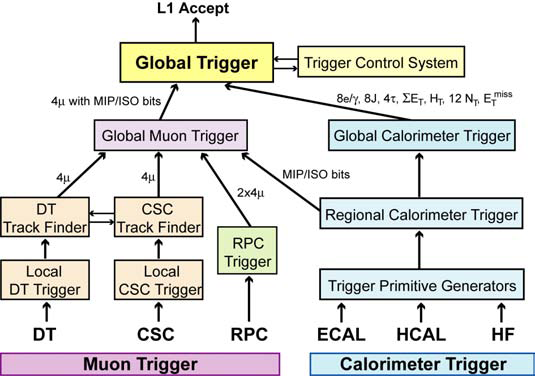
\includegraphics[width=0.95\textwidth]{figures/L1_architecture.png}
\caption{The architecture of the L1 Trigger.}
\label{fig:L1-trigger}
\end{center}
\end{figure}

The HLT further analyzes events which pass the L1A decision. Using a farm of roughly 1000 commercial processors comprised of over 13000 central processing units (CPUs), it approximately emulates the full offline reconstruction algorithms described in Ch. \ref{ch:reconstruction}. Like the L1 Trigger, the HLT uses a set of triggers with different criteria, called the trigger menu. Different trigger menus are constructed for various conditions, including different instantaneous luminosity levels and different types of collisions or measurements. The selected menu can be changed during the operation of the detector in response to new conditions. Events which pass the HLT decision are sorted into primary datasets (PDs) with minimal overlap. The HLT output includes several streams, including monitoring and calibration streams in addition to the primary stream of physics events.

During the 2012 run, the L1 Trigger operated at rates up to 100\unit{kHz} with only 3\% dead time \cite{Brooke:2013hnf}. The HLT operated at rates up to 1\unit{kHz} and took an average of 200\unit{ms} to process an event \cite{Trocino:2014jya}. This processing speed is two orders of magnitude faster than the full offline reconstruction. Around 600\unit{Hz} of HLT output data was ``parked'', or recorded to disk in a raw format before being processed. This data parking scheme took advantage of the impending 2013-2014 long shutdown for collider and detector upgrades, when CPUs would be available to process the extra data. The parked data was collected using alternative trigger menus designed to enable precision measurements and new physics searches in unexplored kinematic regions. CMS also engaged in ``data scouting'', performing simple analyses on partially-reconstructed events, for example keeping only HLT-reconstructed jets, from processes which would normally have rates too high to be accepted by the trigger. These simple analyses searched for noticeable deviations from SM predictions in order to indicate possible advantageous changes to the trigger menus.

\section{Luminosity Measurement}

The fine resolution of the CMS pixel detector (Sec. \ref{sec:tracker}) implies that a given pixel will tend to be activated by one track at most per bunch crossing. A minimum bias interaction creates an average of 200 clusters, with each cluster containing an average of 5 pixels \cite{CMS-PAS-LUM-12-001}. Even with 100 pileup events per bunch crossing, the pixel detector will have an occupancy as low as 0.1\%. The number of pixel hits should thus scale linearly with the number of interactions per bunch crossing for instantaneous luminosities up to and even beyond the LHC design performance. Equation \eqref{eq:pixel-lumi} shows how the instantaneous luminosity $\mathcal{L}$ is related to the average number of pixel clusters per event $\langle n \rangle$ \cite{CMS-PAS-LUM-13-001}:
\begin{equation} \label{eq:pixel-lumi}
\mathcal{L} = \frac{\nu \langle n \rangle}{\sigma_\text{vis}}.
\end{equation}
Here, $\nu = 11246\unit{Hz}$ is the LHC revolution frequency, $\langle n \rangle$ is defined as $\mu n_{1}$ where $\mu$ is the number of collisions per bunch crossing and $n_{1}$ is the average number of clusters per collision, and the visible cross section $\sigma_\text{vis}$ is defined as $\sigma_\text{T} n_{1}$ where $\sigma_\text{T}$ is the total inelastic cross section. A Van der Meer scan is used to calibrate $\sigma_\text{vis}$. In 2012, CMS measured the total integrated luminosity with a systematic uncertainty of 2.6\% using this method.

The HF is used as a second method of measuring the luminosity. This is possible because the HF can be run safely during unstable beams \cite{CMS-PAS-LUM-13-001}. Information from the HF can be used to measure the luminosity in two different ways. The average fraction of empty towers can be related to the mean number of interactions per crossing, or the average transverse energy per tower can be linearly related to the luminosity. It can make an online determination of the average luminosity to a statistical uncertainty of 1\% in under 1\unit{s}. However, the calibration of this measurement can drift over long time periods due to changes in the gain of the HF PMTs. In practice, the increase in pileup interactions observed during the 2012 run moves the HF response into a nonlinear regime, limiting the accuracy of this method. Because of these limitations, the HF method is utilized primarily as a cross-check for the pixel cluster counting method.
% input: [reconstruction.tex]
\chapter{Event Reconstruction
\label{ch:reconstruction}}

Particles created in proton-proton collisions pass through the CMS detector and leave signals in different subdetectors. Figure \ref{fig:cms-slice} shows examples of typical signals for different types of particles. Each type of particle has a different characteristic signature from which it can be identified using information from the various subdetectors. Muons, electrons, and charged hadrons create tracks in the tracker, while photons and neutral hadrons do not. Muons also create hits in the muon systems. Electrons and photons deposit energy in the ECAL, while charged and neutral hadrons deposit most of their energy in the HCAL. Neutrinos do not deposit any energy in the detector. Their presence must be inferred from missing transverse momentum, defined as the negative vector sum of \vecpt for all particles in the event: $\vecmet = - \sum_{i} \vecpt^{(i)}$. The magnitude of this quantity is called the missing transverse energy, denoted as \met. Because the incident proton beams have momentum only in the $z$ direction, any imbalance of measured momentum in the tranverse plane indicates particles which were not detected.

\begin{figure}[hbt]
\begin{center}
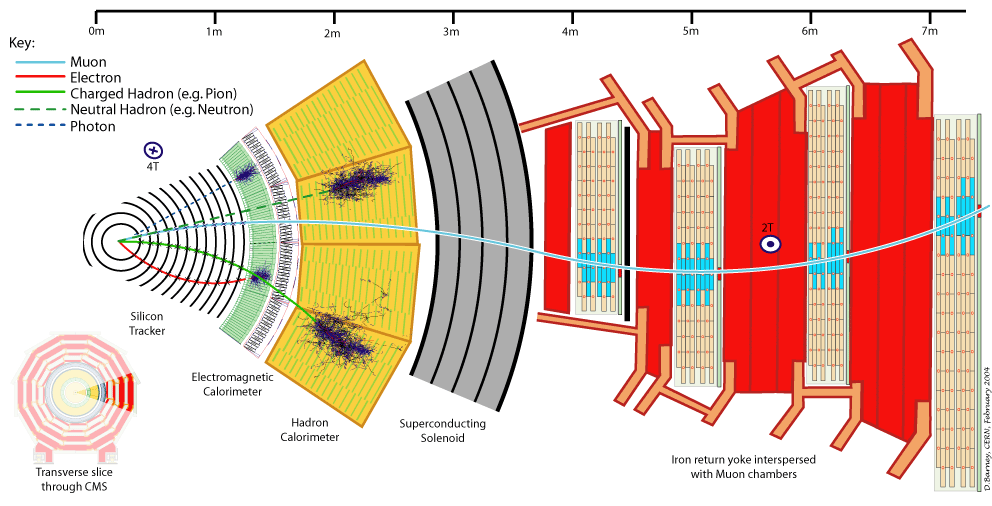
\includegraphics[width=0.95\textwidth]{figures/CMS_slice.png}
\caption{A cross-sectional view of the CMS detector with all subdetectors labeled and examples of signals left by muons, electrons, charged hadrons, neutral hadrons, and photons \cite{CMS-slice}.}
\label{fig:cms-slice}
\end{center}
\end{figure}

The raw output from each subdetector is processed in several steps in order to reconstruct the different types of particles \cite{TDR-software}. The first step is local reconstruction, which involves the creation of reconstructed hits or ``RecHits'' for each subsystem of each subdetector. The tracker RecHits include information about the positions of signals in the form of clusters, which are combinations of contiguous strips or pixels. The muon system RecHits also provide the positions of signals. In the DT and CSC subsystems, these RecHits can be combined into three-dimensional track segments. The ECAL and HCAL RecHits contain the energy, position, and time of energy deposits from traversing particles.

In the second step, global reconstruction, the RecHits from the different subsystems of a given subdetector are combined and further processed. In the tracker, pattern recognition algorithms are employed to reconstruct tracks for various cases, including displaced vertices, low \pt tracks, and high \pt tracks. The ECAL and HCAL RecHits are combined into calorimeter towers or ``CaloTowers'' using a projective $\eta$-$\phi$ geometry. ``Standalone'' muons are created by the muon system global reconstruction, which associates RecHits and track segments in a radial trajectory, accounting for bending by the residual magnetic field, and uses a vertex-constrained fit.

High-level reconstruction is the final step, in which information from all subdetectors is used to reconstruct various types of particles as precisely as possible. The particle types used in this search include electrons, muons, taus, jets, and b-jets. The reconstruction algorithms for these particles will be described in more detail in the following sections of this chapter. Many of these algorithms use a particle flow technique that is unique to CMS and will be described in Sec. \ref{sec:particle-flow}.

The CMS experiment uses detailed simulations to predict the performance of the detector and reconstruction algorithms and to model various physics processes. Each simulated event is generated from the interaction of partons in proton-proton collisions and the decays of the resulting particles, based on theoretical calculations. The traversal of the final state particles through the CMS detector is simulated, and after some processing, the results can be treated identically to the raw data from real events and used as input for the reconstruction software.

\section{Event Generation}

Protons are most basically considered to be composed of two up quarks and one down quark. However, as a QCD bound state, it is more accurate to consider those three quarks as valence quarks, the most prominent features in a quark-gluon sea of virtual particles. At high energies such as those present in LHC collisions, the presence of additional quarks and gluons, collectively called partons, becomes significant. The fraction of the momentum of a proton $A$ carried by a parton $a$ is defined as $x_a$, and the parton distribution function (PDF) for that parton is $f_{a/A}(x_a,Q^2)$, where $Q^2$ is the momentum scale of the interaction, typically the square of the total four-momentum in a collision. PDFs are calculated using experimental data sets, with different groups taking different approaches to analyzing the data and modeling proton behavior. The CMS experiment primarily uses PDFs from Martin-Stirling-Thorne-Watt (MSTW) and the Coordinated Theoretical-Experimental Project on QCD (CTEQ). Figure \ref{fig:pdf-mstw} shows an example set of PDFs calculated at NLO by MSTW \cite{MSTW09}. At high momentum scales, even bottom quarks may be present in the quark-gluon sea of a proton. The dependence of the PDFs on $Q^2$ is given by the Dokshitzer-Gribov-Lipatov-Altarelli-Parisi (DGLAP) equations \cite{QuarkGluon}.

\begin{figure}[hbt]
\begin{center}
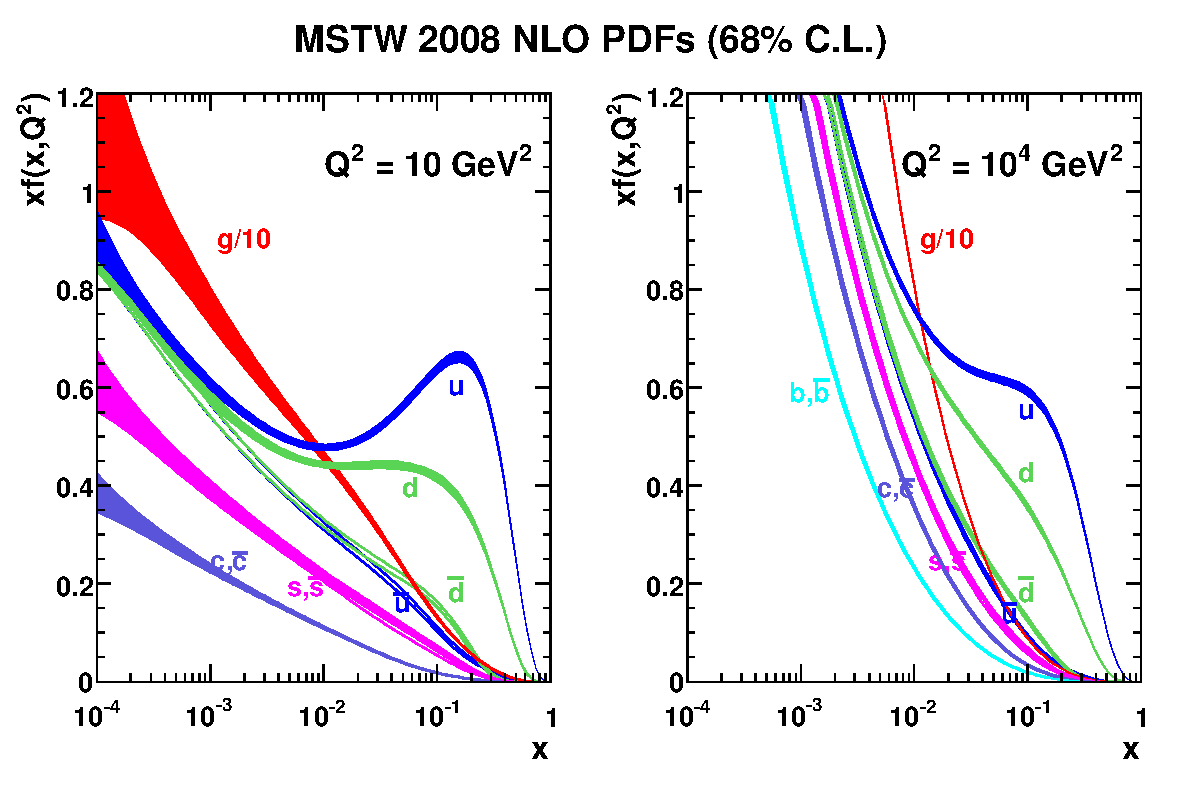
\includegraphics[width=0.95\textwidth]{figures/mstw2008nlo68cl_allpdfs.pdf}
\caption{PDFs calculated at NLO by MSTW, plotted against momentum fraction $x$ for two different values of the momentum scale $Q^2$ \cite{MSTW09}.}
\label{fig:pdf-mstw}
\end{center}
\end{figure}

The DGLAP equations allow large logarithmic factors, for example from col\-lin\-ear emission of gluons, to be included in the definition of the PDFs. This statement is the QCD factorization theorem, which applies to all hard-scattering processes. With this theorem, the interaction of parton $a$ in proton $A$ with parton $b$ in proton $B$, producing the final state $X$, can be written simply:
\begin{equation} \label{eq:hard-scatter}
\sigma_{AB \rightarrow X}(s) = \int{\text{dx}_{a}\text{dx}_{b} f_{a/A}(x_a,\mu_{F}^{2}) f_{b/A}(x_b,\mu_{F}^{2}) \hat{\sigma}_{ab \rightarrow X}(\hat{s},\mu_{R}^{2})}
\end{equation}
For such an interaction at high energy, the center-of-mass energy is $\sqrt{\hat{s}} = \sqrt{x_a x_b s}$, where $\sqrt{s}$ is the center-of-mass energy of the proton-proton system. There are two scales in Eq. \ref{eq:hard-scatter}: the factorization scale $\mu_{F}$ which separates long-distance physics from short-distance physics, and the renormalization scale $\mu_{R}$ of the QCD running coupling. Values for these scales are typically chosen to be characteristic of the hard scattering, with $\mu_{F} = \mu_{R}$. In addition to the primary hard-scattering process, the incoming protons and outgoing final state particles may radiate photons and gluons in processes called, respectively, initial state radiation (ISR) and final state radiation (FSR). The remnant partons which did not participate in the primary hard scatter may undergo soft interactions; these are collectively considered to be the ``underlying event''. All of these possible interactions in a proton-proton collision are visualized in Fig. \ref{fig:pp-collision}.

\begin{figure}[hbt]
\begin{center}
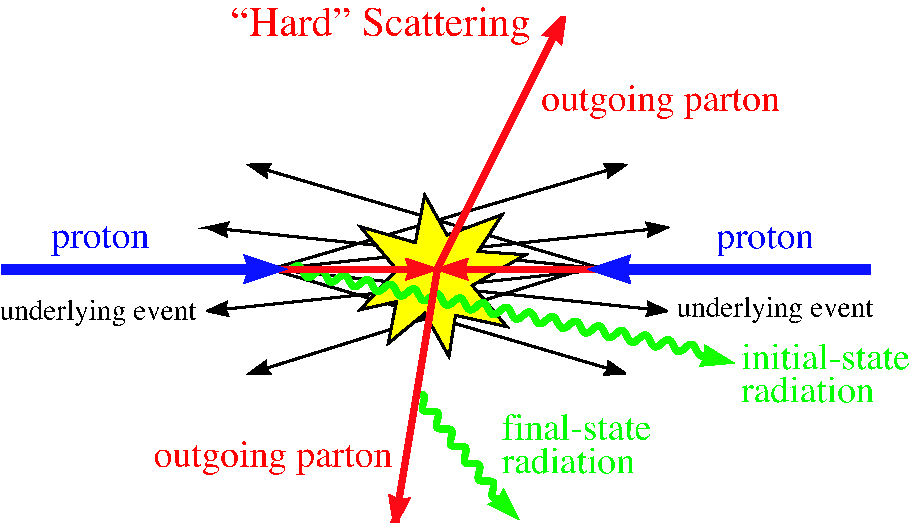
\includegraphics[width=0.95\textwidth]{figures/pp_collision_schematic.pdf}
\caption{An illustration of a proton-proton collision, showing the hard scattering, ISR, FSR, and the underlying event \cite{QuarkGluon}.}
\label{fig:pp-collision}
\end{center}
\end{figure}

Various event generation programs exist to simulate proton-proton collisions. The simulation of the hard scattering relies on a $2\rightarrow2$ matrix element to calculate $\hat{\sigma}_{ab \rightarrow X}(\hat{s},\mu_{R}^{2})$. Usually, the LO matrix element and PDFs are used for the simulation, and the results are scaled to NLO or NNLO using a $K$-factor derived from the ratio of the relevant cross sections. The program \PYTHIA \cite{Sjostrand:2006za} uses a parton showering approach to model ISR and FSR. Other generators such as \MADGRAPH \cite{MadGraph} use alternate approaches which more accurately simulate additional hard radiation outside of the primary hard scattering process, but must be combined with a program like \PYTHIA for showering from soft and collinear radiation. \POWHEG \cite{Alioli:2010xd} is a generator which uses NLO matrix elements and PDFs by matching them with parton shower contributions to prevent double counting. After the initial event generation, \MADGRAPH and \POWHEG are interfaced with \PYTHIA for hadronization. In addition, a specialized program called \TAUOLA \cite{TAUOLA} can be applied for accurate handling of tau lepton decays.

\section{Detector Simulation}

The response of the CMS detector to a proton-proton collision event is simulated using the stable final state particles output by event generators. The progression of each particle through the detector is tracked using the \GEANTfour software \cite{geant4nim,geant4ieee}. The geometry of every subdetector and subsystem is carefully simulated to ensure the accuracy of the simulation. The conditions of the real detector, including alignment and calibration changes, are measured periodically and stored in a database which can be used to configure the simulation. \GEANTfour includes customizable physics lists containing models of various physical processes to simulate the interactions of particles with matter. The detector simulation creates simulated hits or ``SimHits'' for each subdetector from the deposition of energy or charge based on those interactions. The effects of photodetectors and readout electronics on these SimHits are then simulated, mimicing the real subdetectors' data acquisition processes.

\section{Tracks and Vertices
\label{sec:tracks}}

Hits from the different tracker subsystems are reconstructed into charged-particle tracks using the Combinatorial Track Finder (CTF) algorithm \cite{TrackingJINST}. CTF is an iterative algorithm which finds the easiest tracks first, in order to remove the associated hits from consideration. This reduces the complexity of finding more difficult tracks in subsequent iterations. Each iteration follows the same four-step procedure, varying the type of seed used and the selection criteria applied.
\begin{enumerate}
\item A seed is generated using only a few hits.
\item Additional hits are added to the track based on the extrapolated trajectory of the seed.
\item The parameters of the track are estimated using a fit which considers all hits in the trajectory.
\item Selection criteria are applied to determine the quality of the track, and tracks which do not pass the selection are excluded.
\end{enumerate}

The types of seeds are categorized based on the number of hits included and the source of those hits. Initial iterations use pixel triplet and pair seeds, created from three and two pixel hits, respectively. These are the highest-quality seeds and are used to reconstruct prompt tracks, those emitting from primary vertices near the IP. A subsequent iteration uses a mixed triplet seed, containing 1--3 pixel hits and ${<}3$ strip hits. This iteration typically finds displaced tracks from heavy flavor decays, nuclear interactions, and photons which convert to \EpEm\xspace pairs in the tracker. The final iterations use strip pair seeds, consisting of two matched hits from the strip detectors, usually generated by charged particles which did not enter the pixel detector.

The iterations that use seeds with strip hits may also find prompt tracks which lack pixel hits. The specific sequence of iterations has been modified several times to improve the computing and physics performance of CMS tracking \cite{Tracking2012}. Table \ref{tab:tracking} lists the sequence used during the 2012 run. The selection criteria for each iteration are given, including cuts on \pt, transverse impact parameter $d_0$, and longitudinal impact parameter $z_0$. Some of the $z_0$ cuts are in terms of $\sigma$, the length of the beam spot in the $z$-direction used as a Gaussian standard deviation.

\begin{table}[htb]
  \begin{center}
    \begin{tabular}{llllll}
\hline
step  & seed type & seed subdetectors & \pt $[\GeVcns]$ & $d_0$ [cm] & $|z_0|$ \\
\hline
0     & triplet   & pixel             & ${>}0.6$     & ${<}0.02$  & ${<}4.0\sigma$ \\
1     & triplet   & pixel             & ${>}0.2$     & ${<}0.02$  & ${<}4.0\sigma$ \\
2     & pair      & pixel             & ${>}0.6$     & ${<}0.015$ & ${<}0.09\cm$ \\
3     & triplet   & pixel             & ${>}0.3$     & ${<}1.5$   & ${<}2.5\sigma$ \\
4     & triplet   & pixel/TIB/TID/TEC & ${>}0.5$--0.6 & ${<}1.5$   & ${<}10.0\cm$ \\
5     & pair      & TIB/TID/TEC       & ${>}0.6$     & ${<}2.0$   & ${<}10.0\cm$ \\
6     & pair      & TOB/TEC           & ${>}0.6$     & ${<}2.0$   & ${<}30.0\cm$ \\
\hline
    \end{tabular}
    \caption{The sequence of tracking iterations used during the 2012 run, including information on the seeds and selection criteria used in each step \cite{Tracking2012}.}
    \label{tab:tracking}
  \end{center}
\end{table}

The reconstructed tracks are used to reconstruct the primary vertices from the event \cite{TrackingJINST}. This includes both the main hard scatter vertex and additional vertices from pileup collisions. First, selection requirements are imposed on the tracks, in order to consider only prompt tracks near the IP. The selection requirements include cuts on the significance of $d_0$, the number of pixel and strip hits in the track, and the normalized $\chi^2$ from the fit of the track trajectory. The tracks which pass the selection requirements are clustered together using their $z$-coordinates, determined at each track's closest approach to the beam spot. A deterministic annealing algorithm is used to perform this clustering, in which each track may have a different probability to be associated with each vertex. The algorithm uses analogues of statistical mechanics quantities, slowly reducing the ``temperature'' and minimizing the ``free energy'' during each temperature iteration.

Once the deterministic annealing algorithm produces a list of vertex candidates, an adaptive vertex fitter is applied to each vertex candidate. This fitter weights each track in the vertex based on the agreement between the track and vertex positions. Using those weights, it fits the parameters of the vertex, including the $(x,y,z)$ position, the covariance matrix, and the number of degrees of freedom, $n_{\text{dof}} = -3 + 2 \sum{w_i}$, where $w_i$ is the weight for the $i$th track. The variable $n_{\text{dof}}$ can be used to select vertices which correspond to actual proton-proton interactions, as it is closely related to the number of tracks compatible with the vertex.

Several requirements are applied to the reconstructed primary vertices to ensure high quality \cite{CMS-PAS-TRK-10-005}. The number of degrees of freedom $n_{\text{dof}}$ must be greater than 4. The longitudinal position $z$ of the vertex must obey $|z|<24\mm$, and the transverse position $\rho$ must obey $|\rho|<2\mm$. In addition, the vertex must be reconstructed by a fit to tracks. The other reconstructed objects described below can be assigned to a reconstructed vertex. The closest vertex to the track associated with the object is chosen as its vertex. For electrons, the GSF track is used; for muons, the best track is used; and for hadronically decaying tau leptons, the track of the leading charged hadron is used.

%add 2012 performance (efficiency, fake rate, vtx resolution)? references only have 2011 performance...

\section{Particle Flow
\label{sec:particle-flow}}

The CMS experiment uses a technique called particle flow (PF) to combine information from all subdetectors in order to identify all stable particles in each event \cite{CMS-PAS-PFT-09-001}. As described at the beginning of this chapter and shown in Fig. \ref{fig:cms-slice}, each type of stable particle is expected to create signals in a certain subset of the subdetectors. The performance of the PF algorithm was validated using early CMS data \cite{CMS-PAS-PFT-10-002,CMS-PAS-PFT-10-003}, along with newer CMS data for more recent uses of the algorithm \cite{Beaudette:2014cea}, demonstrating significant improvement over simpler approaches. The reconstructed particles are known as PF candidates, which can be treated as input particles by the various high-level reconstruction algorithms. PF candidates can also be used to compute the isolation of a reconstructed object, by summing the energy of candidates topologically close to the selected object.

The RecHits from the local reconstruction process are used to create the basic elements for this technique: tracks and clusters. Charged-particle tracks are created from tracker RecHits using an iterative algorithm as described in Sec. \ref{sec:tracks}, and muon tracks are created from muon system RecHits. Calorimeter energy deposits are grouped into clusters by identifying seed hits as local energy maxima exceeding a certain threshold, and then adding neighboring hits with energy above subsystem-specific thresholds meant to eliminate photodetector noise. Further removal of noise from the calorimeters is performed by rejecting clusters with characteristics matching those expected from leading sources of noise. Tracks and clusters are associated together using a linking algorithm that determines if they were likely produced by the same particle. The algorithm considers a possible link between each algorithm based on the $\eta$-$\phi$ distance between a charged-particle track and a cluster, accounting for propagation in the magnetic field, or between two clusters. For links between a charged-particle track and a muon track, the $\chi^{2}$ value from a global fit is used as the link distance. Groups of elements are associated based on minimizing the link distance and are called ``blocks''.

PF reconstruction algorithms classify the blocks as different types of particles. When a block is classified as a certain type of particle, it is removed from the list of unclassified blocks. A global muon block is accepted as a PF muon if the momentum of the combined charged-particle and muon tracks agrees with the momentum of the charged-particle track alone. The energy expected to have been deposited by the PF muons in the calorimeters due to minimum ionization is subtracted from the clusters. The remaining charged-particle tracks are checked for compatibility with electrons, which tend to leave short tracks and radiate energy via bremsstrahlung. A Gaussian Sum Filter (GSF) is applied to the compatible tracks in order to identify spatially-matched ECAL clusters, and the combination of a track and one or more clusters is classified as a PF electron.

The remaining tracks are linked to clusters to form PF charged hadrons, if the total cluster energy is similar to but smaller than the total track momentum. More than one track can link to a given cluster, but for a given track, only the link to the closest cluster is kept. This reflects the coarser segmentation of the calorimeter system as compared to that of the tracker. In cases where the total cluster energy is significantly smaller than the total track momentum, additional PF muons may be found using tracks from the block, and some tracks may be classified as fake and removed from consideration. Finally, an excess of energy in the clusters, above the total track momentum, is assumed to come from neutral particles. The excess energy is typically classified as a PF photon. If the total excess cluster energy in a block is larger than the total ECAL energy in the cluster, a PF neutral hadron is created from the excess energy remaining after assigning the ECAL excess energy to a PF photon. The remaining clusters not linked to any tracks are used to create PF photons in ECAL and PF neutral hadrons in HCAL.

\section{Electrons
\label{sec:ele-reco}}

The electron candidates reconstructed by the PF algorithm are considered to be ``tracker-driven'' \cite{CMS-PAS-EGM-10-004}. This approach is suitable for low-\pt electrons and electrons produced by jets. For higher-\pt electrons, an alternative ``ECAL-driven'' approach is used. ECAL clusters are grouped into superclusters to account for bremsstrahlung photons radiated by electrons as they traverse the tracker, as well as the spread of energy in the $\phi$-direction due to the magnetic field \cite{ElectronReco}. Similarly to the PF algorithm, these superclusters are matched with track seeds and a GSF is used to reconstruct the trajectory of the electron track. Using a mixture of Gaussians to select the electron track better accounts for the energy loss from bremsstrahlung, as compared to the standard CMS track finding procedure \cite{ElectronGSF}. The lists of tracker-driven and ECAL-driven electron candidates are compared to avoid double counting.

Quality cuts on various kinematic variables are applied to the GSF electron candidates to identify whether or not they are genuine electrons \cite{ElectronCutBased}. A set of cut values is called a working point, and multiple working points are defined based on the strictness of the cut values. The $\eta$ width of the supercluster, $\sigma_{i\eta i\eta}$, is taken from the covariance matrix of the $\eta$ positions of the included crystals compared to the seed cluster. A modified $\eta$ variable which accounts for the crystal spacing is used, and each crystal's contribution is weighted using the logarithm of the ratio of its energy to the seed cluster energy \cite{EgammaShowerShape}. The differences in position of the supercluster, $(\eta_{\text{sc}},\phi_{\text{sc}})$, and the extrapolated track, $(\eta_{\text{in}}^{\text{extrap}},\phi_{\text{in}}^{\text{extrap}})$, are defined as $|\Delta \eta_{\text{in}}| = |\eta_{\text{sc}} - \eta_{\text{in}}^{\text{extrap}}|$ and $|\Delta \phi_{\text{in}}| = |\phi_{\text{sc}} - \phi_{\text{in}}^{\text{extrap}}|$. The leakage energy $H$ in the HCAL tower located behind the ECAL seed cluster is compared to the energy of the seed cluster $E$ in the variable $H/E$. The transverse and longitudinal impact parameters of the vertex associated with the electron, $d_{0}^{\text{vtx}}$ and $z_{0}^{\text{vtx}}$, are used. The variable $|1/E - 1/p|$, comparing the electron energy and momentum, is also considered. Finally, the isolation is computed by summing the \pt of charged hadron (CH), neutral hadron (NH), and photon ($\gamma$) PF candidates within a cone of $\Delta R < 0.3$ of the electron candidate, including a correction for contributions from pileup based on the median energy per area $\rho$ and the effective area of the electron $A_{\text{eff}}$:
\begin{equation}
I^{\text{PF}}_{\Pe} = \sum_{\Delta R < 0.3}{\pt^{(\text{CH})}} + \text{max}\left( \sum_{\Delta R < 0.3}{\pt^{(\text{NH})}} + \sum_{\Delta R < 0.3}{\pt^{(\gamma)}} - \rho A_{\text{eff}}, 0 \right).
\end{equation}
The relative isolation $I^{\text{PF}}_{\Pe}/\pt^{(\Pe)}$, scaled by the \pt of the electron, is used for the quality cuts.

Two working points for the quality cuts described in Sec. \ref{sec:ele-reco} are used to identify reconstructed electrons in this dissertation. Table \ref{tab:eleWP} lists the various requirements for each working point. Electrons are required to be in the barrel with $|\eta|<1.444$ or in the endcap with $1.56<|\eta|<2.5$. The leading electron in the \etau channel is selected with the medium working point. In addition to these quality cuts, it is required to have $\pt>30\GeV$ to match the specifications of the HLT criterion used to collect the primary dataset, as described in Sec. \ref{sec:obsdatasamples}. The loose working point is used to veto additional electrons and for selections in some control regions. The less restrictive kinematic cut $\pt>20\GeV$ is applied to electrons identified with the loose working point.

\begin{table}[htb]
  \begin{center}
    \begin{tabular}{|r|c|c|c|c|}
      \hline
      \multirow{3}{*}{Cut Variable} & \multicolumn{4}{|c|}{Cut Value} \\
      \cline{2-5}
                                    & \multicolumn{2}{|c|}{Medium} & \multicolumn{2}{|c|}{Loose} \\
      \cline{2-5}
                                    & Barrel & Endcap & Barrel  & Endcap    \\
      \hline
      $I^{\text{PF}}_{\Pe}/\pt<$    & 0.15     & 0.15     & 0.15      & 0.15      \\      
      $\sigma_{i\eta i\eta}<$       & 0.01     & 0.03     & 0.01      & 0.03    \\ 
      $|\Delta\phi_{\text{in}}|<$   & 0.06     & 0.03     & 0.15      & 0.10    \\ 
      $|\Delta\eta_{\text{in}}|<$   & 0.004    & 0.007    & 0.007     & 0.009    \\ 
      $H/E<$                        & 0.12     & 0.10     & 0.12      & 0.10     \\ 
      $|d_0^{\text{vtx}}|<$         & 0.02     & 0.02     & 0.02      & 0.02     \\              
      $|d_z^{\text{vtx}}|<$         & 0.1      & 0.1      & 0.2       & 0.2      \\              
      $|1/E - 1/p|<$                & 0.05     & 0.05     & 0.05      & 0.05     \\
      \hline
    \end{tabular}
    \caption{The quality cuts for the medium and loose working points of the electron identification. }
    \label{tab:eleWP}
  \end{center}
\end{table}

\section{Muons
\label{sec:muon-reco}}

The PF muon candidates are used for muon reconstruction. In addition, two supplementary methods are used to reconstruct muons \cite{CMS-PAS-MUO-10-002}. The first method considers all charged-particle tracks from the tracker, above minimal \pt and $p$ cuts, and creates a tracker muon from any track whose extrapolated position matches a track segment in the muon system. This method is efficient for low-momentum muons. The second method produces global muons. This method starts with a standalone muon from a track segment in the muon system and finds a matching track from the tracker. A global muon fit is then performed using both the muon system and tracker tracks, which can provide better momentum resolution for high-\pt muons. The global and track muon candidates, along with any remaining standalone muons which were not matched to a charged-particle track, are combined into one collection in order to prevent double counting.

As with electrons, working points are defined based on sets of quality cuts with different strictness. These cuts can include minimum numbers of muon system hits and segments, as well as minimum numbers of pixel hits and overall tracker hits. The reduced $\chi^2$ from the global muon fit is considered. The distances between the primary vertex and the transverse and longitudinal impact parameters $d_0$ and $d_z$ of the tracker track are also used. The isolation is calculated using PF candidates within a cone of $\Delta R < 0.4$ of the muon:
\begin{equation}
I^{\text{PF}}_{\mu} = \sum_{\Delta R < 0.4}{\pt^{(\text{CH})}} + \text{max}\left( \sum_{\Delta R < 0.4}{\pt^{(\text{NH})}} + \sum_{\Delta R < 0.4}{\pt^{(\gamma)}} - \Delta\beta \sum_{\Delta R < 0.4}{\pt^{(\text{PU})}}, 0 \right).
\end{equation}
A $\Delta\beta$ pileup (PU) correction is applied using the \pt of PU particles, which are identified as charged PF candidates from a different vertex than the muon. The $\Delta\beta$ factor is assigned a value of 0.5 based on the expected ratio of charged to neutral particles in pileup \cite{CMS-PAS-PFT-10-002}. Again, cuts are made on the relative isolation $I^{\text{PF}}_{\mu}/\pt^{(\mu)}$. The selections on these quantities are intended to minimize the contribution from cosmic ray muons, muons from heavy flavor decays, and leakage from hadronic showers. They also ensure precise measurement of the muon \pt.

Two working points for these quality cuts are used to identify reconstructed muons in this dissertation. Table \ref{tab:muonWP} lists the various requirements for each working point. The leading muon in the \mutau channel is selected with the tight working point. In addition to these quality cuts, it is required to have $\pt>30\GeV$ and $|\eta|<2.1$ to match the specifications of the HLT criterion used to collect the primary dataset, as described in Sec. \ref{sec:obsdatasamples}. The loose working point is used to veto additional muons and for selections in some control regions. Less restrictive kinematic cuts $\pt>20\GeV$ and $|\eta|<2.4$ are applied to muons identified with the loose working point.

\begin{table}[htb]
  \begin{center}
    \begin{tabular}{|l|l|}
\hline
\multicolumn{2}{|c|}{Working Point}\\
\hline
\multicolumn{1}{|c|}{Tight} & \multicolumn{1}{c|}{Loose} \\
\hline
PF muon & PF muon \\
Global muon & Global muon OR tracker muon \\
$\begin{aligned}
I^{\text{PF}}_{\mu}/\pt &< 0.12 \\
d_0 &< 0.2\cm \\
d_z &< 0.5\cm \\
\text{Global track fit } \chi^2/n_{\text{dof}} &< 10 \\
\text{Global track fit } n_{\text{muon segment}} &> 0 \\
n_{\text{hits}}(\text{pixel}) &> 0 \\
n_{\text{layers}}(\text{tracker}) &> 5 \\
n_{\text{stations}}(\text{muon}) &> 1
\end{aligned}$
&
$\begin{aligned}
I^{\text{PF}}_{\mu}/\pt &< 0.3 \\
\\
\\
\\
\\
\\
\\
\\
\end{aligned}$ \\
\hline
    \end{tabular}
    \caption{The quality cuts for the tight and loose working points of the muon identification.}
    \label{tab:muonWP}
  \end{center}
\end{table}

\section{Jets
\label{sec:jet-reco}}

Due to QCD confinement, strongly interacting particles, quarks and gluons, cannot exist in a bare state. They immediately form multiple color singlet bound states, hadrons, using the energy from the gluon field in a process called hadronization. These hadrons tend to be produced in a narrow spray, which is called a jet \cite{Salam:2009jx}. To reconstruct a jet, the component particles must be clustered together. CMS uses the anti-\kt algorithm \cite{Cacciari:2008gp} to perform this clustering. This algorithm is a specific case of a generalized iterative cone algorithm, using the following equations:
\begin{align}
d_{ij} &= \text{min}(p_{\text{T}i}^{2p},p_{\text{T}j}^{2p})\frac{\Delta R_{ij}^{2}}{R^{2}}, \\
\Delta R_{ij}^{2} &= (\eta_i - \eta_j)^2 + (\phi_i - \phi_j)^{2}, \\
d_{iB} &= p_{\text{T}i}^{2p}.
\end{align}
Two distance variables are defined: the distance between particles $i$ and $j$, $d_{ij}$, and the distance between particle $i$ and the beam, $d_{iB}$. These distances are weighted by the \pt of the particles as indicated, and $R$ is a size parameter. At each iteration, both distance variables are calculated for all particles. If the minimum distance is $d_{iB}$, particle $i$ is considered to be a fully-clustered jet and removed from the list of particles. Otherwise, particles $i$ and $j$ from the minimum $d_{ij}$ are grouped together in the particle list. The algorithm continues to iterate until the particle list is empty. The anti-\kt algorithm is a special case of these equations with parameter $p=-1$. It has many desirable properties, including infrared and collinear safety, and the creation of circular jets with radius $R$ as shown in Fig. \ref{fig:ak5-example}.

\begin{figure}[hbt]
\begin{center}
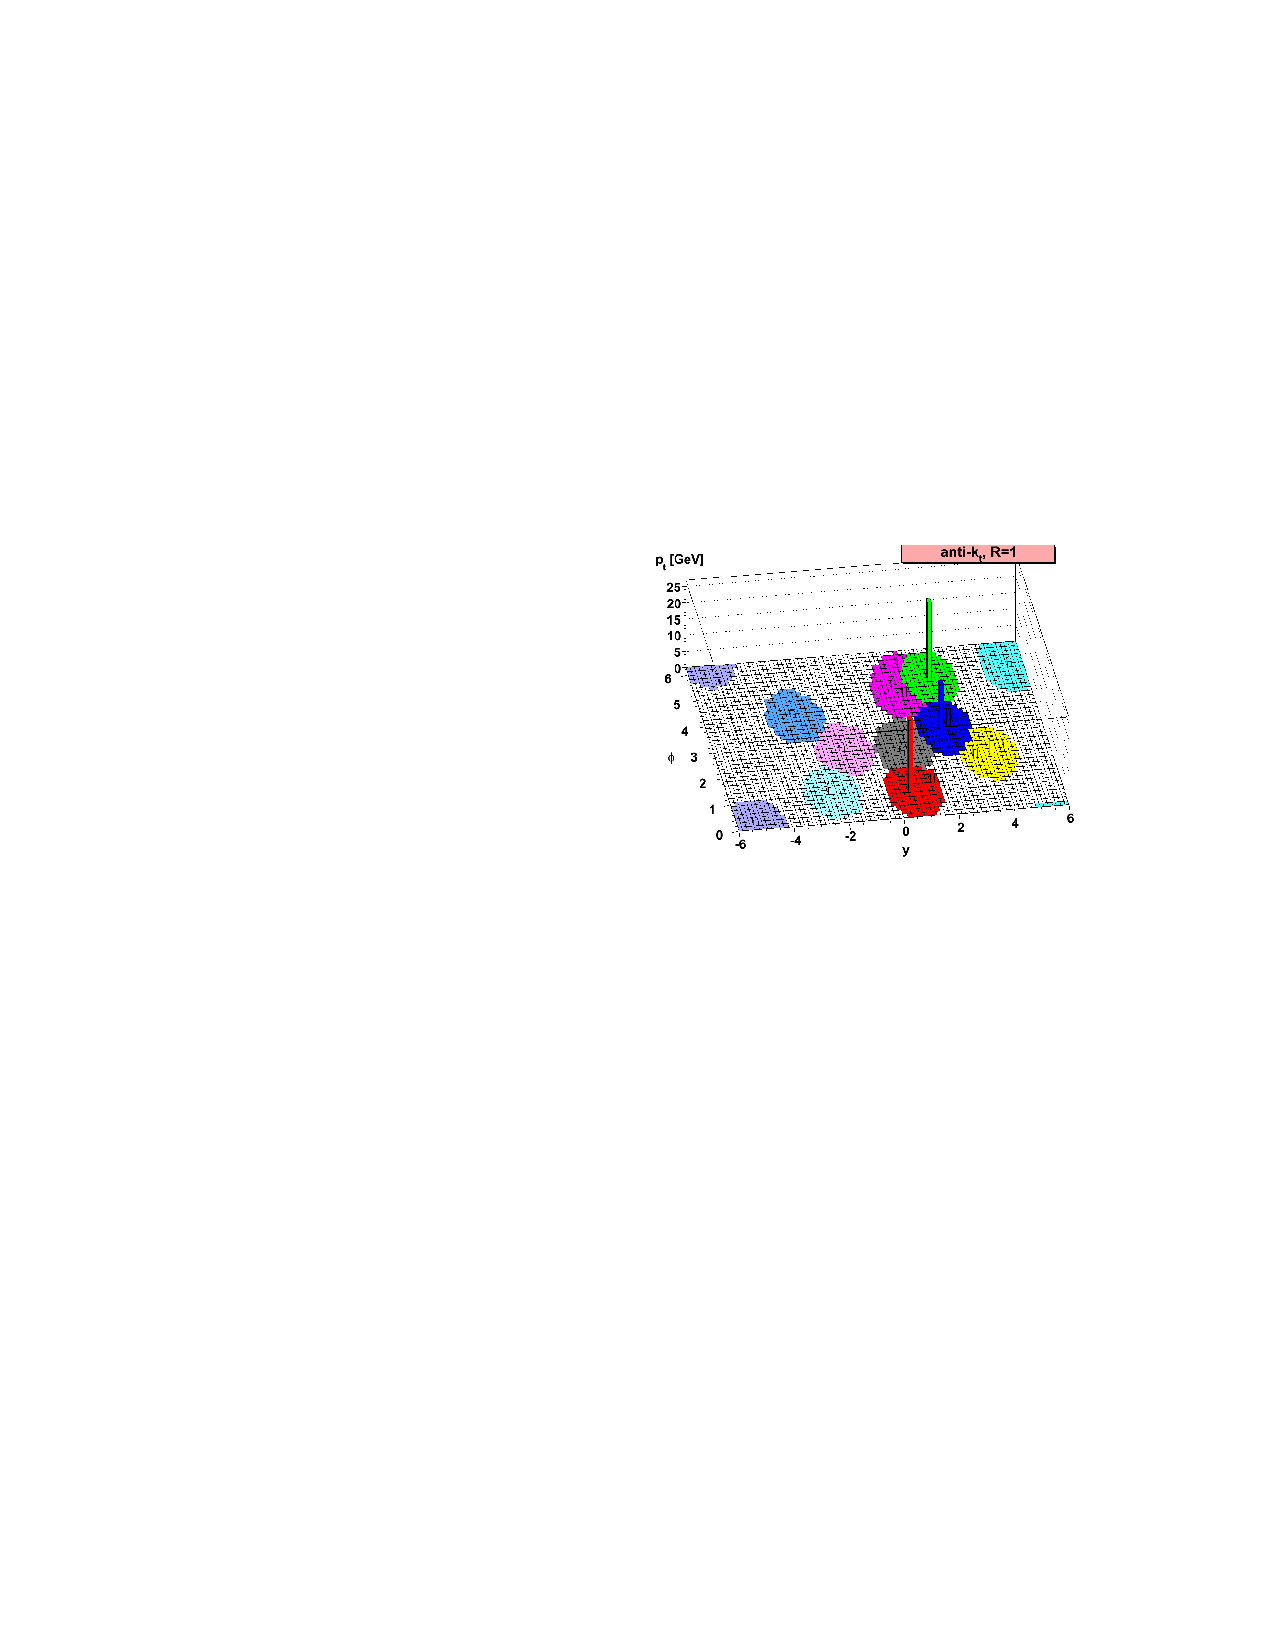
\includegraphics[width=0.95\textwidth]{figures/08021189v2-fig.pdf}
\caption{An example of jets reconstructed with the anti-\kt algorithm, demonstrating the characteristic circular shape \cite{Cacciari:2008gp}.}
\label{fig:ak5-example}
\end{center}
\end{figure}

CMS chooses the value $R = 0.5$ for the size parameter and uses PF candidates for clustering, producing PF jets \cite{CMS-PAS-PFT-09-001, CMS-PAS-PFT-10-002}. Alternative jet methods use CaloTowers and charged-particle tracks separately or together, but these do not perform as well as PF jets. Typically, 65\% of jet energy goes into charged particles, 25\% goes into photons, and 10\% goes into neutral hadrons. Using PF candidates takes advantage of the excellent energy and position resolution for charged particles and photons provided by the combination of the tracker and the calorimeters in the PF algorithm.

Once a jet is reconstructed, several important types of corrections are applied to its energy response \cite{CMS-JEC}. First, minimum bias events are used to estimate the contributions from electronic noise and pileup, and those are subtracted in the offset correction. Next, the energy response is made uniform in $\eta$ using the multiplicative relative correction, derived from dijet events. Finally, the multiplicative absolute correction is derived from \GZJ events, exploiting the precise energy resolution of the ECAL and the tracker, and applied to make the energy response uniform in \pt.

To ensure the quality of reconstructed jets used in data analysis, a set of variables is used for PF jet identification \cite{CMS-AN-2010-003}. These variables include: the fraction of neutral hadrons in the jet $f_{\text{NH}}$, the fraction of neutral EM particles $f_{\gamma}$, the fraction of charged hadrons $f_{\text{CH}}$, the fraction of charged EM particles $f_{\text{EM}}$, the number of constituents $n_{\text{constituents}}$, and the multiplicity of charged particles $n_{\text{charged}}$. Multiple sets of cuts on these variables are defined as working points \cite{PFJetID}. The loose working point of the PF jet identification algorithm is used to identify reconstructed jets in this dissertation. The requirements for the loose working point are summarized in Table \ref{tab:jetWP}. To eliminate jets from pileup interactions, each selected jet is required to have $\pt>30\GeV$. The cut $|\eta|<2.4$ is also applied, in order to include only jets measured in the best-performing regions of the detector.

\begin{table}[htb]
  \begin{center}
    \begin{tabular}{|r|c|}
      \hline
      \multirow{2}{*}{Cut Variable} & Cut Value \\
      \cline{2-2}
                                    & Loose \\
      \hline
      $f_{\text{CH}}>$              & 0.0 \\
      $f_{\text{NH}}<$              & 0.99 \\
      $f_{\gamma}<$                 & 0.99 \\
      $f_{\text{EM}}<$              & 0.99 \\
      $n_{\text{charged}}>$         & 0 \\
      $n_{\text{constituents}}>$    & 1 \\
      \hline
    \end{tabular}
    \caption{The quality cuts for the loose working point of the jet identification. }
    \label{tab:jetWP}
  \end{center}
\end{table}

\section{Taus
\label{sec:hpstau}}

Tau leptons decay into hadrons approximately 64.76\% of the time \cite{PDG}. These hadronic decays produce objects similar to jets, but typically narrower and more isolated. For this reason, PF jets are used as the basis for reconstructing hadronically decaying tau leptons (hadronic taus or $\tauh$s). The Hadron Plus Strips (HPS) algorithm is used to identify tau leptons \cite{TauPerfCMS,Calabria:1516071}. The vast majority of \tauh decays consist of a tau neutrino $\nu_{\tau}$, one or three charged hadrons $h^{-}$ that are either $\pi^{-}$ or $K^{-}$, and zero or more neutral hadrons $\pi^{0}$ that almost immediately decay to two photons. The HPS algorithm only considers the visible decay products, so the $\nu_{\tau}$ is ignored. Table \ref{tab:tauh-decay} lists the leading hadronic decays, including intermediate hadronic resonances when present.

\begin{table}[htb]
  \begin{center}
    \begin{tabular}{|l|l|l|l|}
\hline
Decay                                                       & Resonance   & Mass (\MeVccns) & Branching fraction (\%) \\
\hline
$\tau^{-} \rightarrow h^{-} \nu_{\tau}$                     &             &                 & 11.53\% \\
$\tau^{-} \rightarrow h^{-} \pi^{0} \nu_{\tau}$             & $\rho^{-}$  & 775             & 25.95\% \\
$\tau^{-} \rightarrow h^{-} \pi^{0} \pi^{0} \nu_{\tau}$     & $a_{1}^{-}$ & 1230            & 9.52\% \\
$\tau^{-} \rightarrow h^{-} h^{+} h^{-} \nu_{\tau}$         & $a_{1}^{-}$ & 1230            & 9.80\% \\
$\tau^{-} \rightarrow h^{-} h^{+} h^{-} \pi^{0} \nu_{\tau}$ &             &                 & 4.76\% \\
\hline
    \end{tabular}
    \caption{The leading hadronic decays of tau leptons, including branching fractions and intermediate hadronic resonances \cite{PDG}. The symbol $h^{-}$ can be either $\pi^{-}$ or $K^{-}$. }
    \label{tab:tauh-decay}
  \end{center}
\end{table}

The strips in the HPS algorithm consist of PF photon candidates. Starting with the most energetic photon in the PF jet, the strip is built using an iterative search for other photons within a range $0.20\times0.05$ in $\eta$-$\phi$ around the center of the strip. Each iteration accepts the most energetic photon found and then recalculates the four-momentum of the updated strip. The strip is complete once no remaining photons are found in the given window, and it is kept if it passes a minimum \pt cut. The procedure is repeated with any remaining ungrouped photons in the jet. The formation of strips from photons accounts for spreading of their energy due to the effect of the magnetic field on conversions in the tracker.

Using the constituents of the PF jet, all combinations of strips with one or three charged hadrons are tested, with the charged hadrons assumed to be pions. All strips and charged hadrons must be found within a cone of $\Delta R = \text{max}(\text{min}(0.10,3.0/\pt^{\tauh}),0.05)$, where $\pt^{\tauh}$ is the \pt of the \tauh candidate in \GeVns. Several decay mode topologies are included in the algorithm, with mass ranges enforced for candidates based on the expectation of hadronic resonances in decays \cite{CMS-AN-2014-008}. Figure \ref{fig:tau-modes} shows a simple diagram of the different topologies.
\begin{enumerate}
\item Single hadron, when no strips are found.
\item One hadron + one strip, when the $\pi^0$ decay creates one strip from two narrowly separated photons. The invariant mass of the \tauh candidate, $M_{\tauh}$, must be in the range $0.3 < M_{\tauh} < \text{max}(1.3,\text{min}(1.3\sqrt{\pt^{\tauh}/200},2.1))\GeV$.
\item One hadron + two strips, when the $\pi^0$ decay creates one strip from two narrowly separated photons. In this case, the invariant mass of the two strips combined, $M_{\text{strips}}$, must be in the range $50 < M_{\text{strips}} < 200\MeV$, and $M_{\tauh}$ must be in the range $0.4 < M_{\tauh} < \text{max}(1.2,\text{min}(1.2\sqrt{\pt^{\tauh}/200},2.0))\GeV$.
\item Three hadrons, which requires all three charged hadron candidates to originate from the same primary vertex and to have the appropriate electric charges. $M_{\tauh}$ must be in the range $0.8 < M_{\tauh} < 1.5\GeV$.
\end{enumerate}
If more than one combination of PF constituents passes these decay mode finding requirements, the combination with the highest $\pt^{\tauh}$ is selected.

\begin{figure}[hbt]
\begin{center}
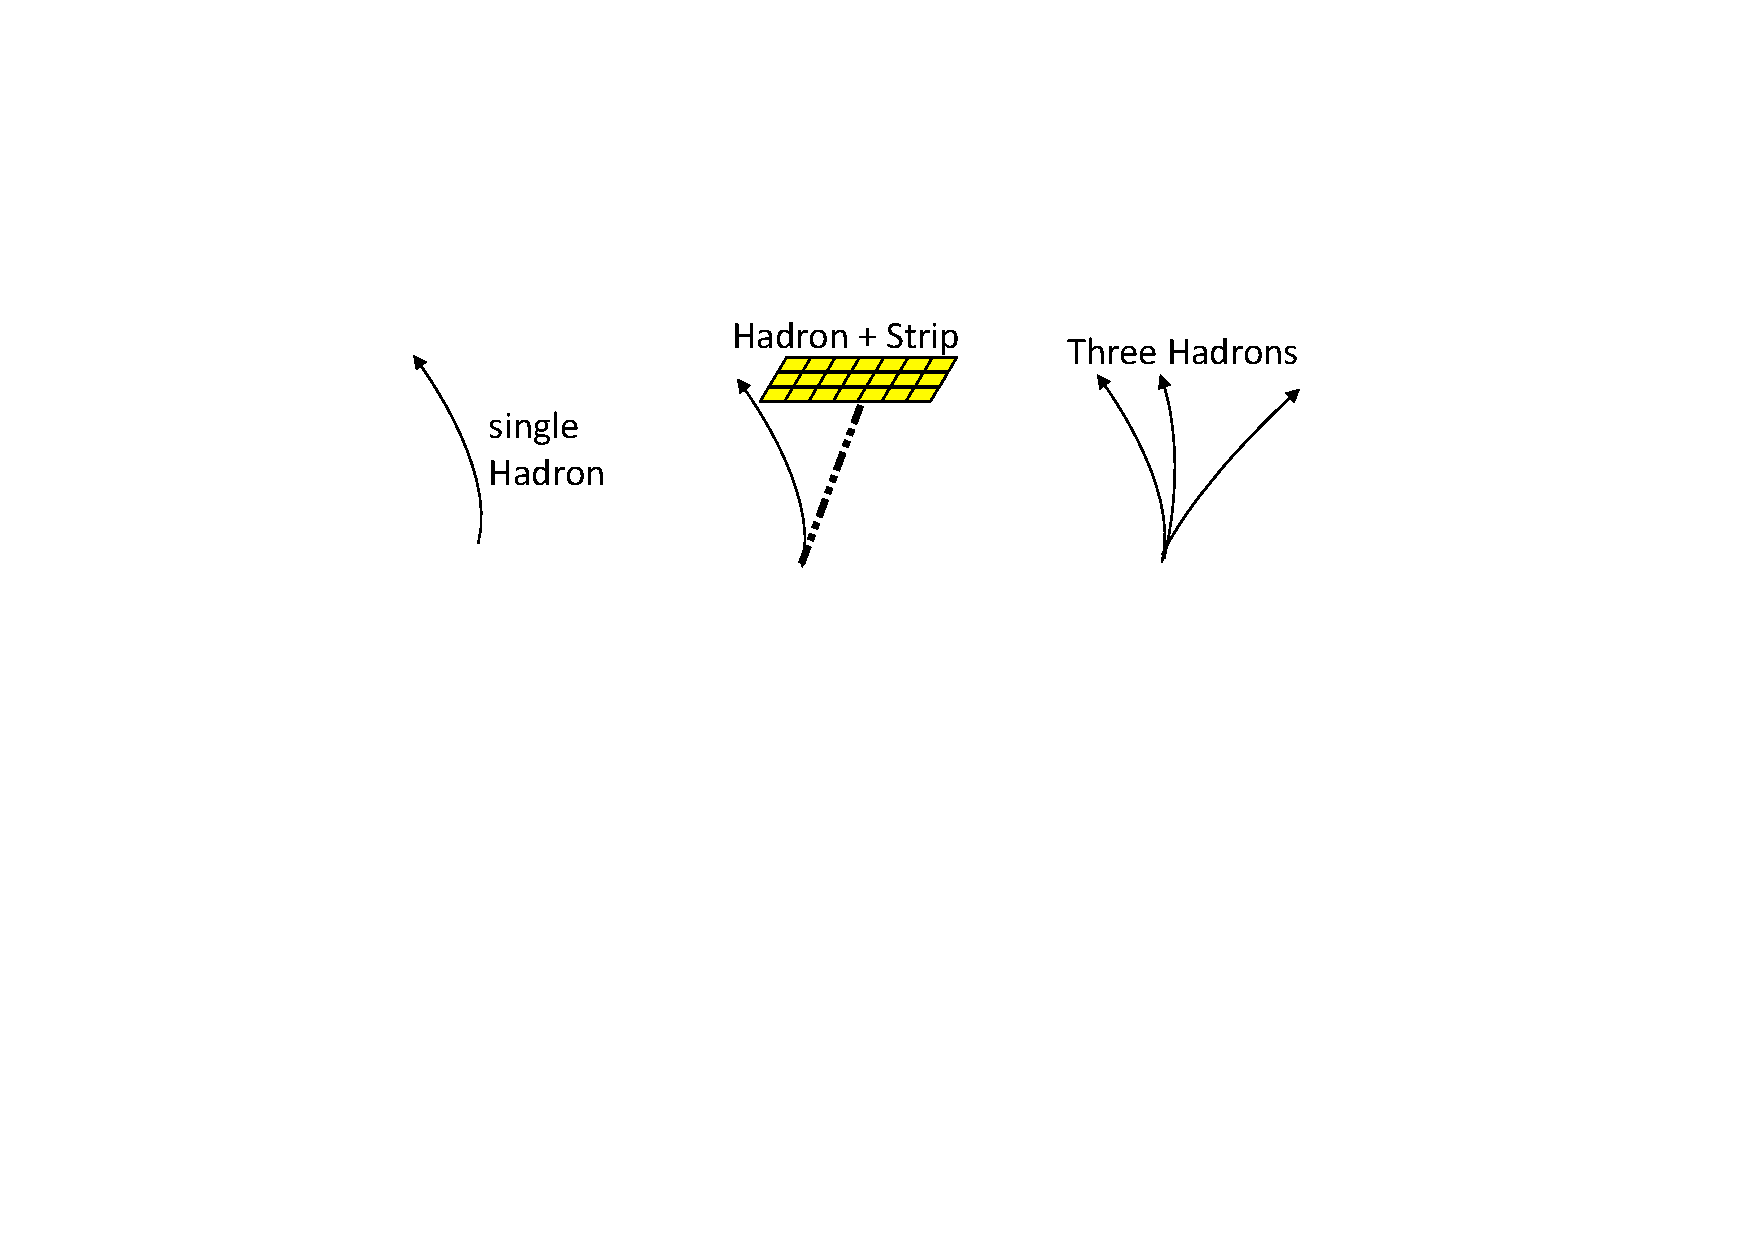
\includegraphics[width=0.95\textwidth]{figures/DP2014_015-fig.pdf}
\caption{A simple diagram of the different hadronic tau decay mode topologies reconstructed by the HPS algorithm \cite{CMS-DP-2014-015}.}
\label{fig:tau-modes}
\end{center}
\end{figure}

Isolation is an important tool in discriminating between $\tauh$s and jets. The isolation variable is computed using charged hadron and photon PF candidates within a cone of $\Delta R < 0.5$ around the \tauh candidate. A $\Delta\beta$ PU correction is applied using PU particles within a cone of $\Delta R < 0.8$ which originate from a different vertex than the \tauh candidate, with the factor $\Delta\beta = 0.4576$ \cite{CMS-DP-2014-015}.
\begin{equation}
I^{\text{PF}}_{\tauh} = \sum_{\Delta R < 0.5}{\pt^{(\text{CH})}} + \text{max}\left( \sum_{\Delta R < 0.5}{\pt^{(\gamma)}} - \Delta\beta \sum_{\Delta R < 0.8}{\pt^{(\text{PU})}}, 0 \right).
\end{equation}
The HPS algorithm uses the absolute isolation $I^{\text{PF}}_{\tauh}$ for the different working point quality cuts. The isolation discrimination also requires that each track associated with the \tauh contain at least three hits in the tracker. In addition to isolation, it is necessary to discriminate against electrons and muons which are misidentified as $\tauh$s. The electron-tau discriminator uses a multivariate (MVA) approach, training boosted decision trees (BDTs) using numerous variables depending on different cases of \tauh. These cases include: the possible association of the primary charged hadron in the \tauh with a GSF track; the possible association of the \tauh with a GSF electron within a cone of $\Delta R < 0.3$; whether or not the \tauh includes strips; and whether the \tauh $\eta$ coordinate lies in the EB or EE range. Multiple trainings for the anti-electron MVA discriminator were performed and multiple working points are defined. The muon-tau discriminator uses a cut-based approach, with multiple sets of cuts and working points defined. The cuts include requirements to minimize the activity in the muon system in the direction of the \tauh and to veto MIP muons based on energy and momentum. 
%The \tauh candidate must not match any muon track segments or any hits in the two outermost muon stations within a cone of $\Delta R < 0.5$. In the single hadron decay mode, the charged hadron in the \tauh must have $(E_{\text{ECAL}} + E_{\text{ECAL}})/p_{\text{track}} > 0.2$.

In this dissertation, the working points for each discriminator can differ for each channel, as listed in Table \ref{tab:tauWP}. The loose working point for the combined isolation requires $I^{\text{PF}}_{\tauh}<2\GeV$. A tighter working point for the muon-tau discriminator is used in the \mutau channel to increase the rejection of muons misidentified as tau leptons from, e.g., the $\Z \rightarrow \mu\mu$ process. The loose working point for the electron-tau discriminator was found to be optimal for both channels. In addition to these discriminators, each reconstructed tau lepton is required to have $\pt>30\GeV$ and $|\eta|<2.3$.

\begin{table}[htb]
  \begin{center}
    \begin{tabular}{|c|c|c|}
      \hline
      \multirow{2}{*}{Discriminator} & \multicolumn{2}{|c|}{Working Point} \\
      \cline{2-3}
                                    & \etau & \mutau \\
      \hline
      Isolation                     & Loose (3 hits)   & Loose (3 hits) \\
      $\Pe$-$\tau$                  & Loose MVA (v3)   & Loose MVA (v3) \\
      $\mu$-$\tau$                  & Loose (v2)       & Tight (v2) \\
      \hline
    \end{tabular}
    \caption{The working points for the different tau discriminators used in the tau lepton identification. }
    \label{tab:tauWP}
  \end{center}
\end{table}

\section{b-tagging
\label{sec:b-tagging}}

Bottom quarks are associated with many interesting physical signatures, including decays of top quarks and Higgs bosons, as well as many BSM theories, including supersymmetry, that privilege or otherwise relate to third-generation fermions. Jets generated by bottom quark hadronization, b-jets, can be identified using certain properties which set them apart from jets from lighter quarks or gluons \cite{BTV-12-001}. Bottom quarks form hadrons with relatively long lifetimes whose decay products tend to have high \pt. Numerous algorithms have been created to identify b-jets based on information from tracks or reconstructed secondary vertices from b-hadron decays. The most successful of these algorithms is the Combined Secondary Vertex (CSV) algorithm, which uses secondary vertices and adds information from the tracks. The CSV algorithm calculates a likelihood-based discriminator to separate b-jets and other jets. Loose, medium, and tight working points are defined for this discriminator, based on setting the probability of misidentifying a light quark or gluon jet as a b-jet to be 10\%, 1\%, and 0.1\%, respectively \cite{CMS-PAS-BTV-13-001}. In this dissertation, the loose working point is used to select b-tagged jets, which requires the discriminator calculated by the CSV algorithm to have a value greater than 0.244.

For a given jet, the CSV algorithm subjects the tracks within that jet to additional purity requirements, beyond those specified in Sec. \ref{sec:tracks}. The track must fall within a cone of $\Delta R < 0.3$ relative to the direction of the jet and the distance between the track and the jet at closest approach must be less than 0.07\cm. The track must include at least two pixel hits and at least eight total tracker hits, with $\chi^2/n_{\text{dof}} < 5$. The impact parameters between the track and the primary vertex must satisfy $d_0 < 0.2\cm$ and $d_z < 17\cm$. Finally, the track must have $\pt>1\GeVc$ and decay length less than 5\cm, where decay length is the distance between the primary vertex and the closest approach of the track and the jet. The significance of the track's impact parameter $S_{\text{ip}}$, defined as the value of the impact parameter divided by its uncertainty, is a powerful observable. The number of high-quality tracks in the jet is also used.

Secondary vertices are reconstructed using the adaptive vertex fitter, which was described in Sec. \ref{sec:tracks}. Candidates are rejected if ${\geq}65\%$ of their tracks are also associated with the primary vertex; if they are outside a cone $\Delta R < 0.5$ with respect to the jet direction; or if they are radially separated from the primary vertex by more than 2.5\cm with an invariant mass close to the $\cmsSymbolFace{K}^{0}$ mass. The CSV algorithm assigns jets into one of three categories based on the presence of a secondary vertex: real vertex, pseudo-vertex, and no vertex. In the pseudo-vertex case, the algorithm uses tracks with $S_{\text{ip}} > 2$ to create an effective secondary vertex when the adaptive vertex fitter fails. In the no vertex case, the algorithm defaults to use only the track-based variables described previously. Otherwise, the vertex variables used include:
\begin{itemize}
\item The significance of the flight distance between the secondary and primary vertices in the transverse plane.
\item The mass of the secondary vertex.
\item The number of tracks in the secondary vertex.
\item The ratio between the energy in the secondary vertex tracks and the energy in all the tracks in the jet.
\item The $\Delta\eta$ values between each the secondary vertex track and the jet.
\item The transverse impact parameter significance for the track that pushes the invariant mass of the secondary vertex above 1.5\GeVcc, the threshold for charm quarks. This is calculated by sorting the tracks by $S_{\text{ip}}$ and combining them one by one.
\end{itemize}
% input: [analysis.tex]
\chapter{Data Analysis
\label{ch:analysis}}

% input: [samples.tex]
\section{Data Samples}

\subsection{Observed Data
\label{sec:obsdatasamples}}

The observed data analyzed in this dissertation consist of 19.712\fbinv of integrated luminosity, collected by the CMS detector during the 2012 run of the LHC. Figure \ref{fig:lumipublic-dqm} shows the total delivered, recorded, and validated integrated luminosity over time throughout the 2012 run. Events are included in the validated data only if the LHC and the CMS detector were fully operational when the event was recorded. The single electron and single muon primary datasets, listed in Table \ref{tab:data-samples}, are used for the \etau and \mutau channels, respectively. Within the single electron dataset, events are selected if they pass the HLT criterion HLT\_Ele27\_WP80, which requires a reconstructed electron with $\pt>27\GeV$ using the identification working point with 80\% efficiency. Similarly, in the single muon dataset, events are selected if they pass the HLT criterion HLT\_IsoMu24, which requires an isolated reconstructed muon with $\pt>24\GeV$. The average number of interactions per bunch crossing was 21 \cite{LumiPublic}.

\begin{figure}[hbt]
\begin{center}
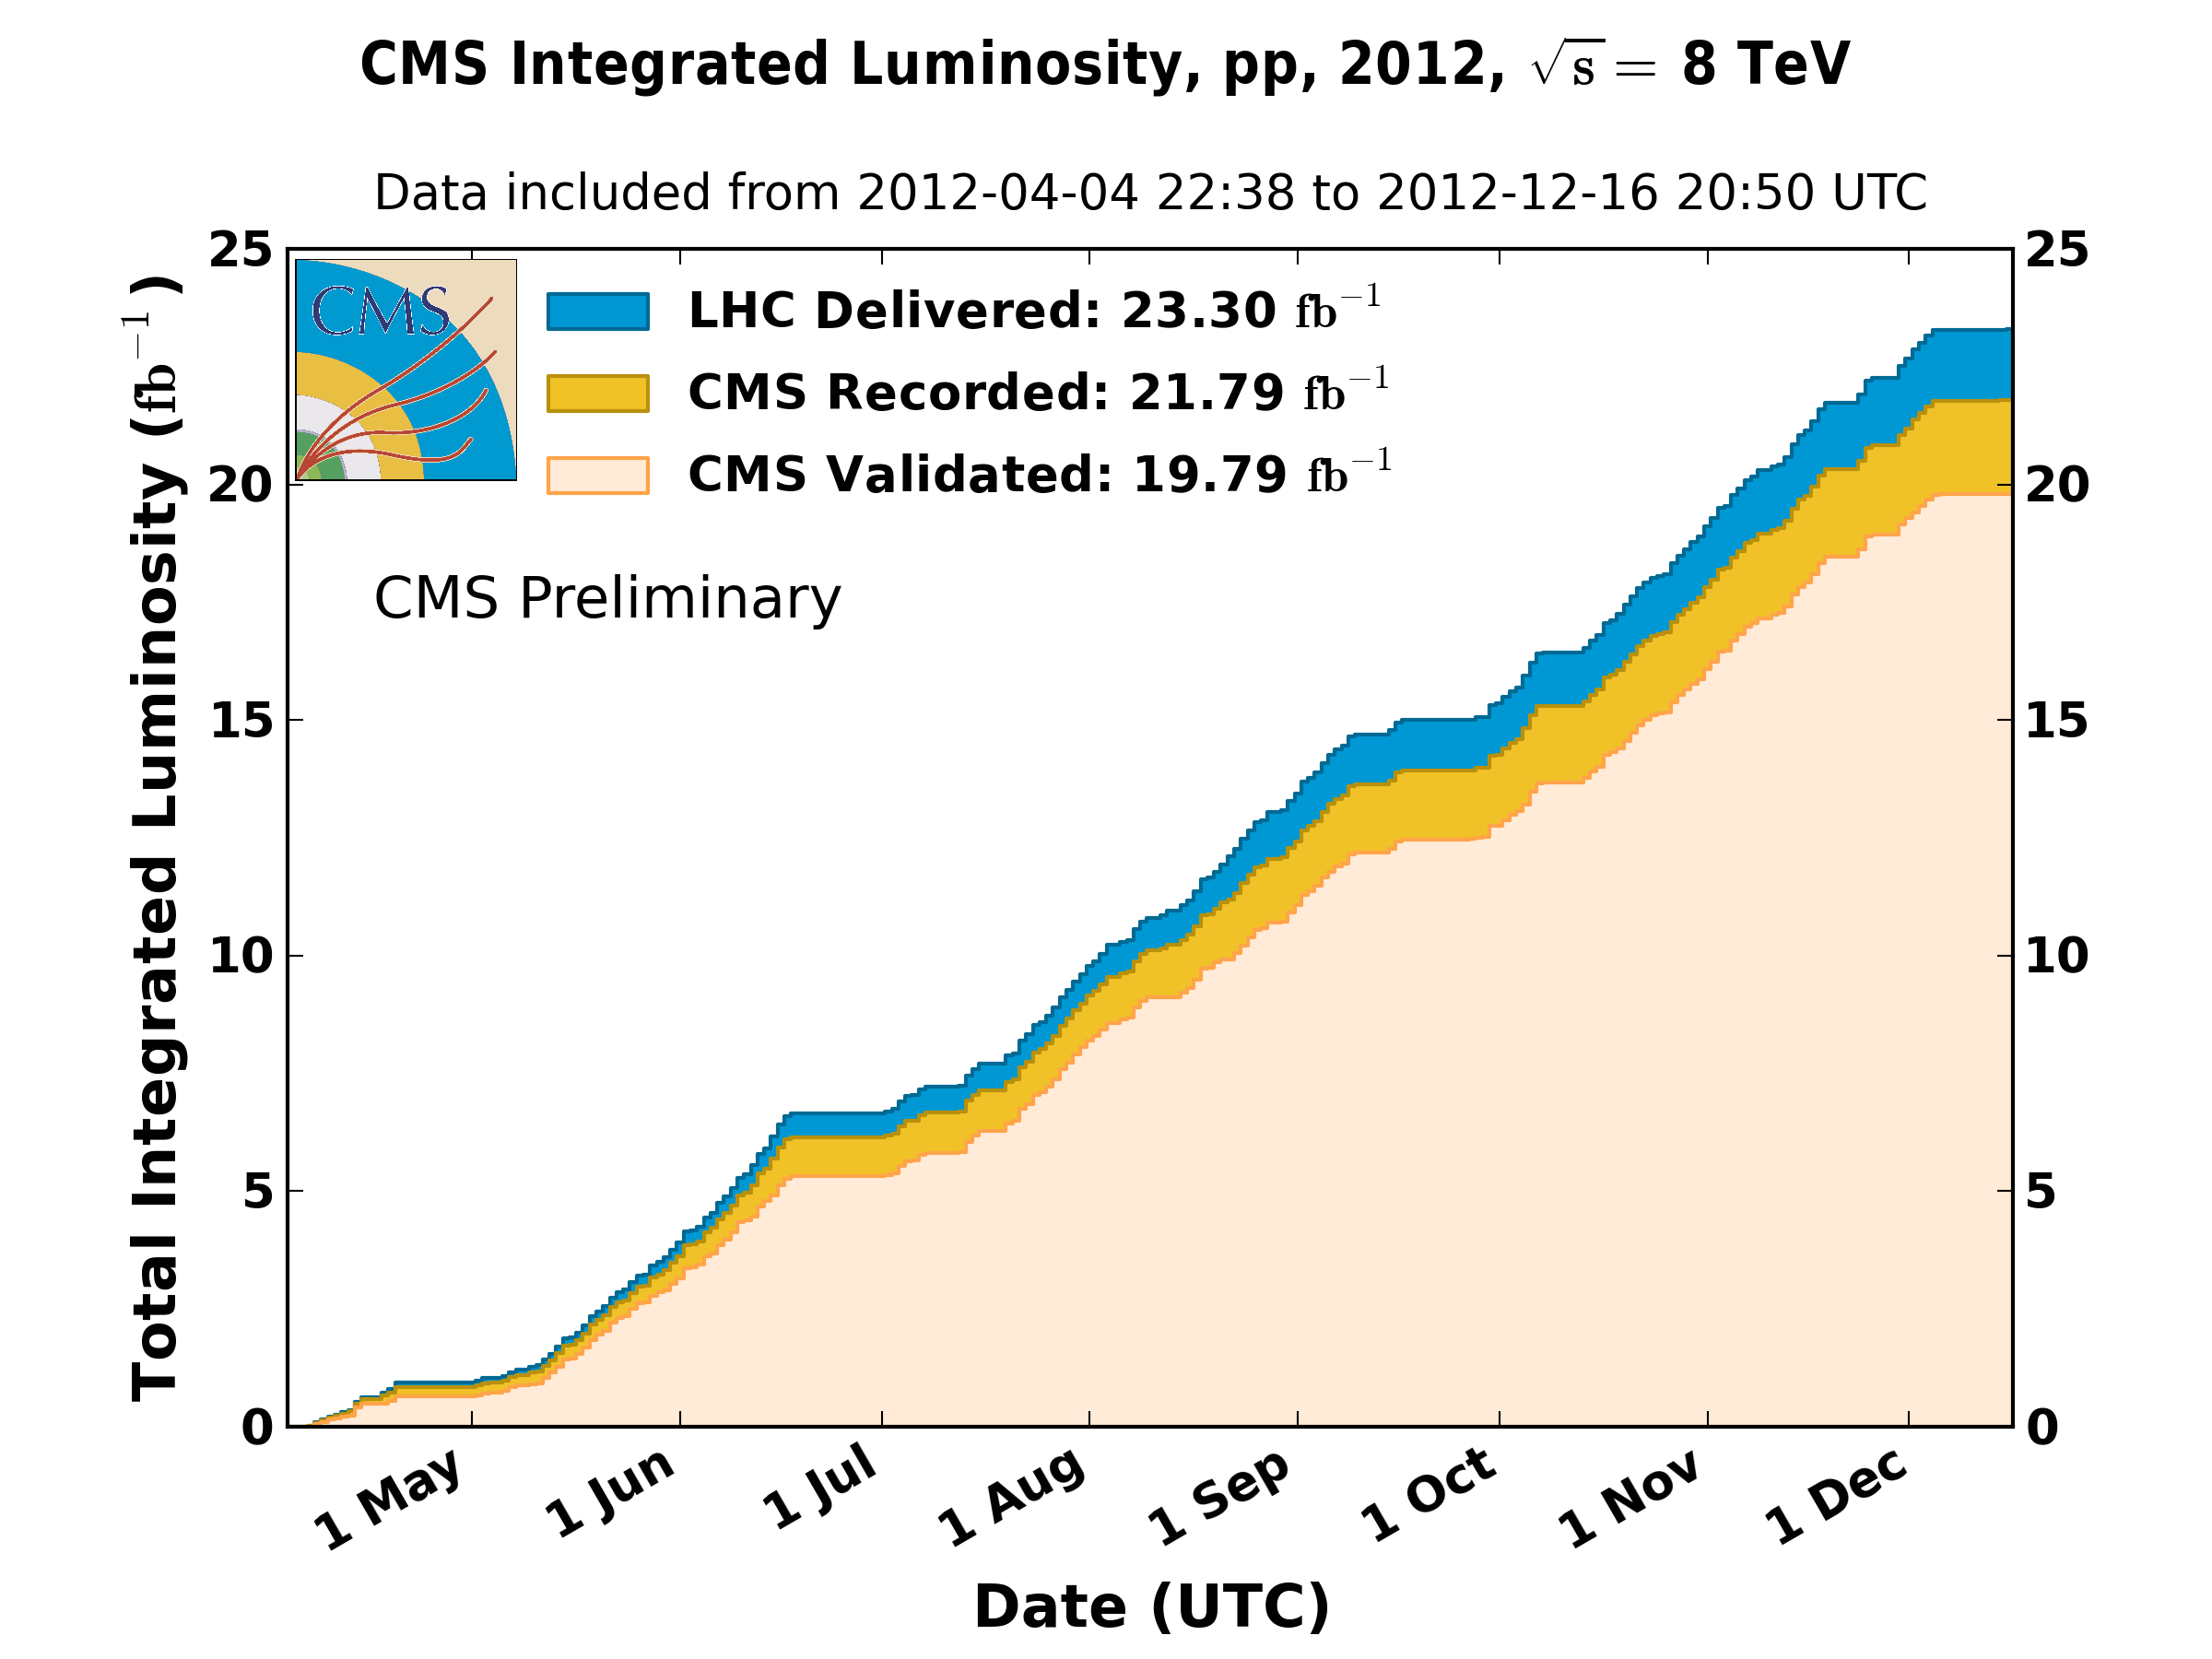
\includegraphics[width=0.95\textwidth]{figures/int_lumi_per_day_cumulative_pp_2012_SummerConf.png}
\caption{A plot of the total integrated luminosity over time for the 2012 run of the LHC, showing the luminosity delivered by the LHC (blue), recorded by the CMS detector (dark orange), and validated as good for physics analysis (light orange) \cite{DataQuality}.}
\label{fig:lumipublic-dqm}
\end{center}
\end{figure}

\begin{table}[hbt]
\begin{center}
\begin{tabular}{|l|}
\multicolumn{1}{c}{$\etau$ channel} \\
\hline
Dataset Name \\
\hline
/SingleElectron/Run2012A-22Jan2013-v1/AOD \\
/SingleElectron/Run2012B-22Jan2013-v1/AOD \\
/SingleElectron/Run2012C-22Jan2013-v1/AOD \\
/SingleElectron/Run2012D-22Jan2013-v1/AOD \\
\hline
\multicolumn{1}{c}{$\mutau$ channel} \\ 
\hline
Dataset Name \\
\hline
/SingleMu/Run2012A-22Jan2013-v1/AOD \\
/SingleMu/Run2012B-22Jan2013-v1/AOD \\
/SingleMu/Run2012C-22Jan2013-v1/AOD \\
/SingleMu/Run2012D-22Jan2013-v1/AOD \\
\hline
\end{tabular}
\caption{The list of observed data samples used in each channel.}
\label{tab:data-samples}
\end{center}
\end{table}

\subsection{Monte Carlo}

Monte Carlo (MC) simulation is used to study the SM background processes which can mimic the signatures of the signal processes. For some processes, the MC simulation is used for the estimation of the final yields and kinematic distributions. For other processes, the final yields and/or kinematic distributions may be estimated from control regions in the observed data. More details on the final background estimations are provided in Sec. \ref{sec:background}. The leptoquark and top squark signal processes are also modeled using MC. A full list of the MC samples used in this dissertation can be found in App. \ref{ch:datasets}.

The \MADGRAPH v5.1.3.30 generator \cite{MadGraph} is used to model the \ttbar, \W + jets, and \Z + jets processes. This generation includes contributions from heavy-flavor and extra jets. For the \ttbar process, an inclusive sample is generated including all decay modes of the two \W bosons from the top quark decays. Exclusive samples with larger numbers of events are also generated, each including only one of three categories for the \W decays: fully leptonic, semileptonic, and fully hadronic. For the \W + jets and \Z + jets processes, inclusive samples including any number of jets are generated. Exclusive samples with larger numbers of events are also generated separately for events with 1 jet, 2 jets, 3 jets, and 4 jets. The single top quark production is modeled with the \POWHEG 1.0 r138 \cite{POWHEG2,POWHEG:singlet,POWHEG:singletW} generator. The \PYTHIA v6.4.24 generator \cite{Sjostrand:2006za} is used to model the diboson processes, including the production of $\W^{+}\W^{-}$, $\Wpm\Z$, and $\Z\Z$, collectively denoted as VV. Both the \MADGRAPH and \POWHEG generators are interfaced with \PYTHIA for hadronization and showering. The \TAUOLA program~\cite{TAUOLA} is used for tau lepton decays in all processes which produce genuine tau leptons. The cross sections for the \ttbar and single top quark processes are calculated at next-to-next-to-leading logarithmic (NNLL) accuracy \cite{TOPCrossSec}. The cross sections for the inclusive \W + jets and \Z + jets processes are calculated at NNLO accuracy, while the cross sections for the exclusive production with a specific number of jets are calculated at LO accuracy \cite{FEWZ}. For the VV processes, the cross sections are calculated at NLO accuracy \cite{MCFM}.

The leptoquark and top squark signal processes are generated using \PYTHIA v6.4.24 \cite{Sjostrand:2006za}. The leptoquark pair production process is generated for $\MLQ=200\GeV$ to $\MLQ=1000\GeV$ in steps of 50\GeV, with the decay $\text{LQ} \rightarrow \tau \cPqb$ required. The cross section for leptoquark pair production is calculated at NLO accuracy \cite{LQxsec}. The theoretical uncertainties on these cross sections have been discussed in Sec. \ref{sec:LQ} and are listed in Table \ref{tab:lq-xsec}. As mentioned in Sec. \ref{sec:RPVSUSY}, the deviation between these LQ production cross sections and the corresponding top squark production cross sections is less than 2\%, so the same cross sections can be used to normalize the samples for both signals. The simulation of the chargino-mediated $\lambda_{3jk}^{\prime}$ decay of the top squark is summarized in Table \ref{tab:LQD321-samples}. Samples are generated for $\Mstop=200\GeV$ to $\Mstop=900\GeV$ in steps of 100\GeV. The MSSM parameters for the event generation are $M_1=1000\GeV$, $M_2=1000\GeV$, $M_3=1500\GeV$, $m_{\sLep}=1500\GeV$, $m_{\sQua}=1500\GeV$, $m_{\sNu}=2000\GeV$ and $\text{tan}(\beta)=40$. Here, $M_1$ is the bino mass term, $M_2$ is the wino mass term, and $M_3$ is the gluino mass term. The $\lambda_{321}^{\prime}$ coupling is selected for the generation; because reconstructed light-quark jets are generally indistinguishable regardless of the flavor of the initial quark, these samples can be used to model signals for all $\lambda_{3jk}^{\prime}$ couplings with $j,k=1,2$.

\begin{table}[htb]
  \begin{center}
    \begin{tabular}{|c|c|c|c|r|}
\hline
$\Mstop$ $[\GeVns]$    &    $M_{\chipm}$ $[\GeVns]$    &   $\mu$ $[\GeVns]$  & $\lambda_{321}^{\prime}$ & \multicolumn{1}{c|}{$N_{\text{events}}$} \\
\hline \hline
200   &      100   &  100.98 & 1  &   539,000   \\
300   &      200   &  201.69 & 1  &   50,000   \\
400   &      300   &  302.49 & 1  &   50,000   \\
500   &      400   &  403.46 & 1  &   50,000   \\
600   &      500   &  504.73 & 1  &   50,000   \\
700   &      600   &  606.55 & 1  &   50,000   \\
800   &      700   &  709.47 & 1  &   50,000   \\
900   &      800   &  815.16 & 1  &   50,000   \\
\hline
\end{tabular}
\caption{A summary of the generation of signal samples for the chargino-mediated $\lambda_{3jk}^{\prime}$ decay of the top squark. The chargino mass is determined by the value of $\mu$.}
\label{tab:LQD321-samples}
\end{center}
\end{table}

To account for known discrepancies between the MC simulation and the observed data, various correction factors are applied to the simulated samples. Corrections for the efficiency of muon trigger criteria, identification, and isolation are calculated using tag and probe methods \cite{MuonRefEffs}. Similar correction factors are calculated for electrons \cite{EgammaTagAndProbe,EgammaScaleFactors}. These correction factors depend on the lepton $\pt$ and $\eta$. The chosen working points for the hadronic tau lepton discriminators were found not to need any corrections in the simulation \cite{TauID}. Correction factors for b-tagging and mistagging efficiencies are applied using the method called ``event reweighting using scale factors and MC b-tagging efficiencies'' with the EPS13 prescription \cite{BTagSFMethods}.

% input: [selection.tex]
\section{Selection and Optimization}

The events analyzed in this dissertation are selected based on requirements for the numbers and types of different reconstructed objects and the relationships between those objects within each event. The selection criteria are applied in three stages. The most basic criteria are applied first in the preselection. This stage is used to validate the Monte Carlo background simulations by examining various relevant kinematic distributions. Second, additional criteria are applied in the main selection, which more closely addresses the expected properties of signal events. Kinematic distributions in the main selection are used to optimize the cuts for the final selection, in order to reduce the contributions from background while enhancing the signal. These optimizations maximize the expected limit from the MC background simulations. Separate final selections are defined for the leptoquark search and the top squark search.

\subsection{Preselection}

At the preselection stage, a single primary well-identified light lepton $\ell$ is required. In the \etau channel, this is an electron satisfying the medium working point and kinematic criteria described in Sec. \ref{sec:ele-reco}. In the \mutau channel, this is a muon satisfying the tight working point and kinematic criteria described in Sec. \ref{sec:muon-reco}. In addition to the light lepton, the event must contain a hadronic tau identified by the HPS algorithm and associated discriminators as defined in Sec. \ref{sec:hpstau}. The two objects, light lepton and hadronic tau, must have opposite charges, originate from the same vertex, and be separated by $\Delta R > 0.5$. Two jets are also required, satisfying the loose working point and kinematic criteria described in Sec. \ref{sec:jet-reco}. The jets must be separated from the light lepton and the hadronic tau by $\Delta R > 0.5$.

Several cases of additional light leptons are vetoed. To suppress background from the \Z + jets process, events are rejected if they contain additional light leptons satisfying the loose working point and having the same flavor and opposite charge with respect to the primary lepton. This separates the contributions from the $\Z \rightarrow \ell\ell$+jets process into control regions which will be used for background estimation. To avoid overlap between the two channels, events are rejected if they contain additional light leptons satisfying the primary working point and kinematic criteria for leptons (medium for electrons and tight for muons) and having the opposite flavor and opposite charge with respect to the primary lepton. This also defines an \emu control region which will be used for background estimation.

Figures \ref{fig:preseletau} and \ref{fig:preselmutau} compare the observed data to the MC background simulation after the preselection in the \etau and \mutau channels, respectively. All histograms in this dissertation show the overflow, if any, in the last bin. The event yields for the observed data and the expected SM backgrounds after the preselection are summarized in Table \ref{tab:eventyieldpresel}. The discrepancy between the observed data and simulated background yields in the \etau channel is due to the presence of QCD multijet events in the observed data. This discrepancy is primarily observed at low \pt and high $\eta$, as expected from QCD. This process is not modeled in the MC simulation because of the difficulty in simulating enough events to be comparable to the amount of data collected by the CMS experiment in 2012. Instead, the yield from QCD is estimated using a same-sign/opposite-sign method which is described in detail in Sec. \ref{sec:qcdbkg}.

\begin{figure}[hbtp]
  \begin{center}
    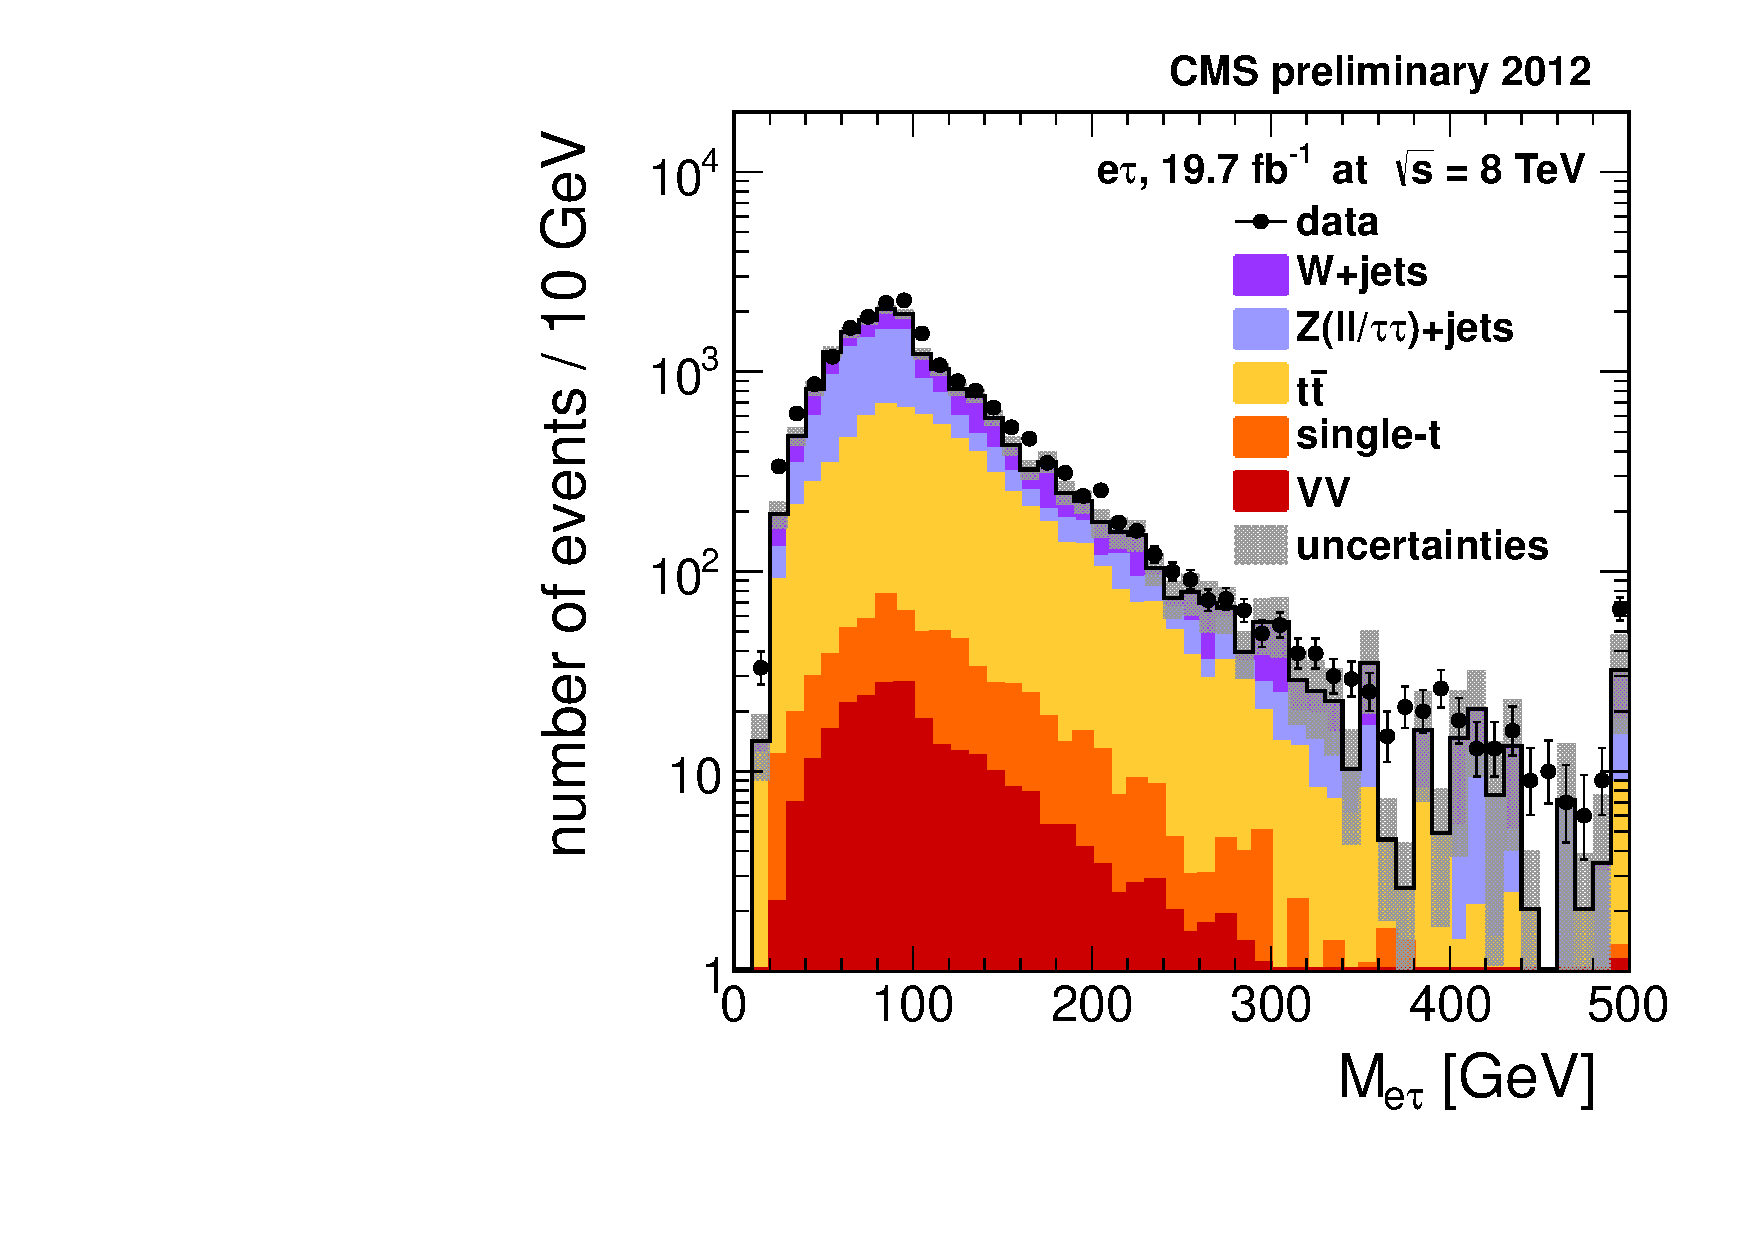
\includegraphics[width=0.465\textwidth]{figures/etau/etauMassMultJet.pdf}
    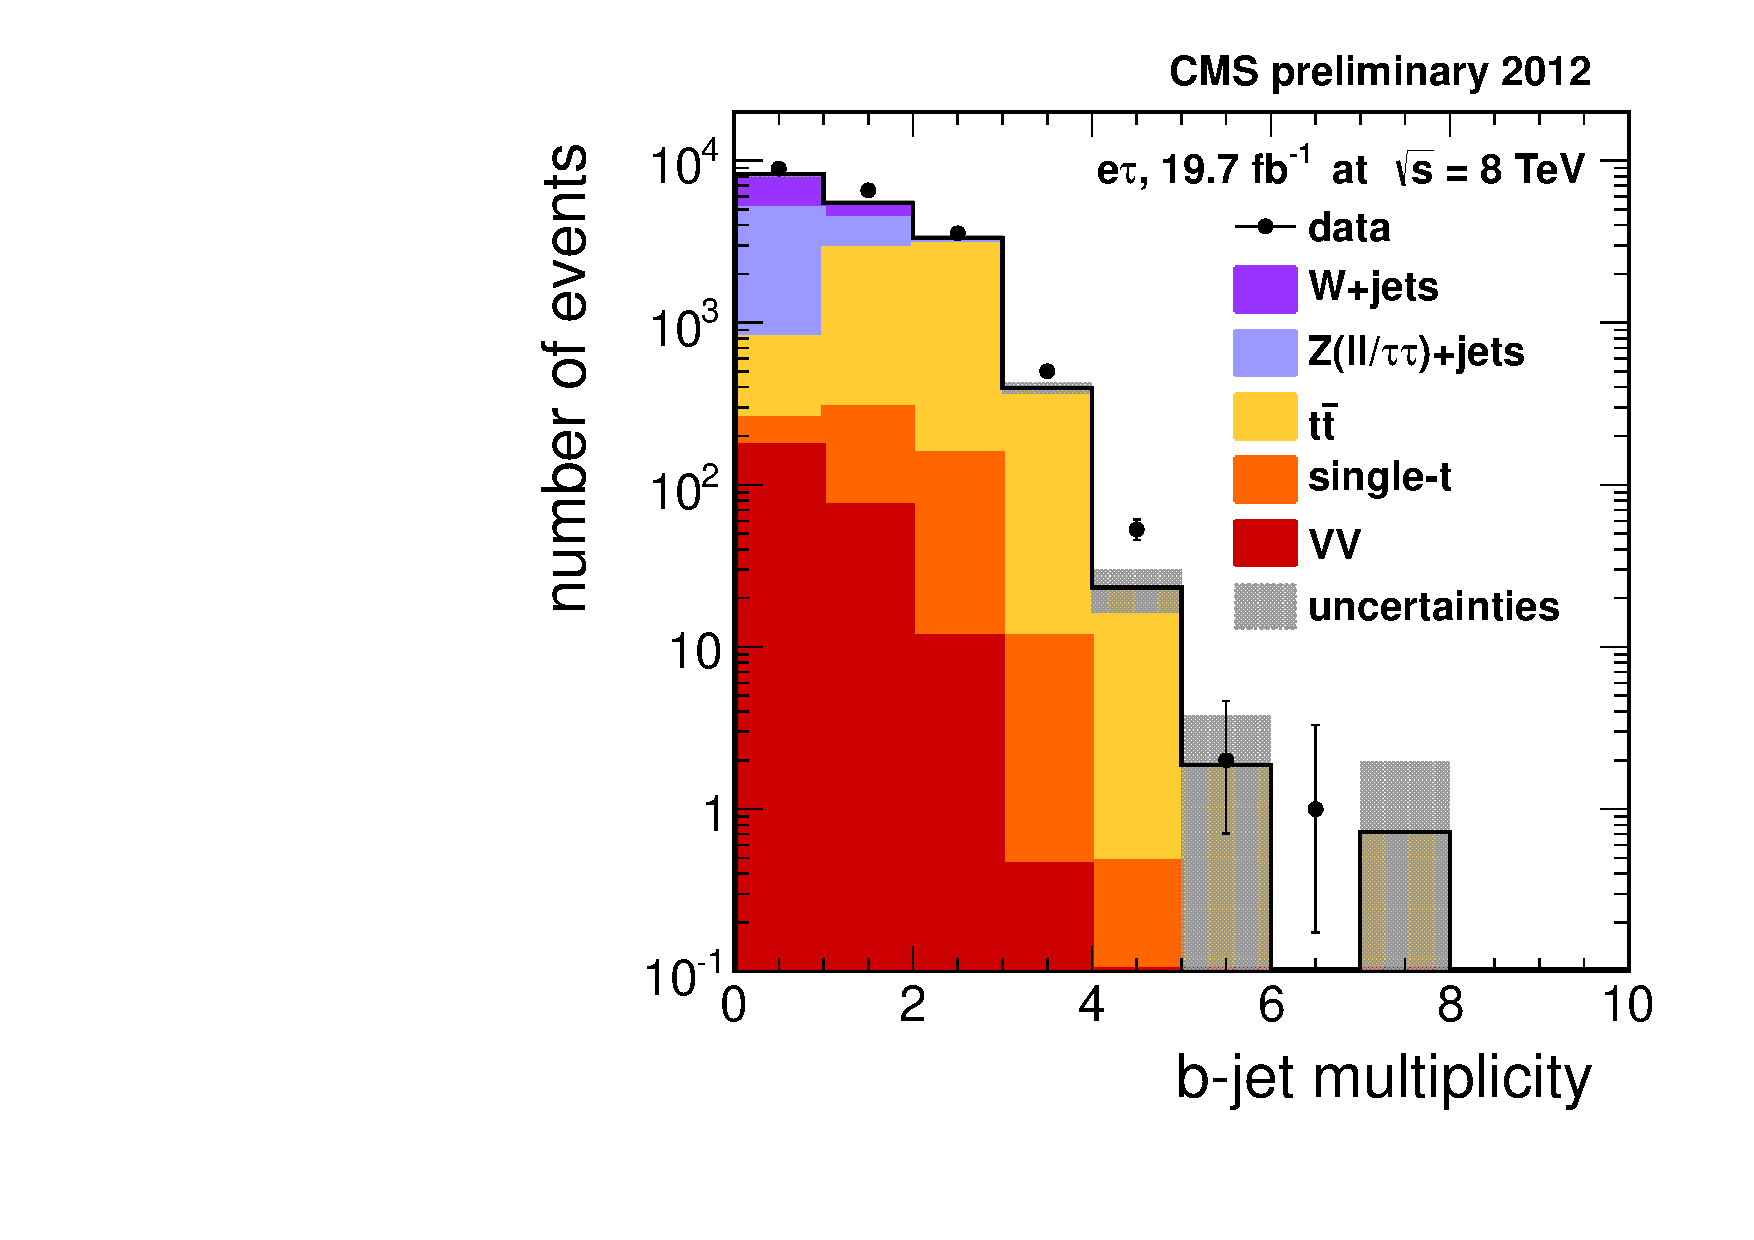
\includegraphics[width=0.465\textwidth]{figures/etau/nBJetMultJet.pdf} \\
    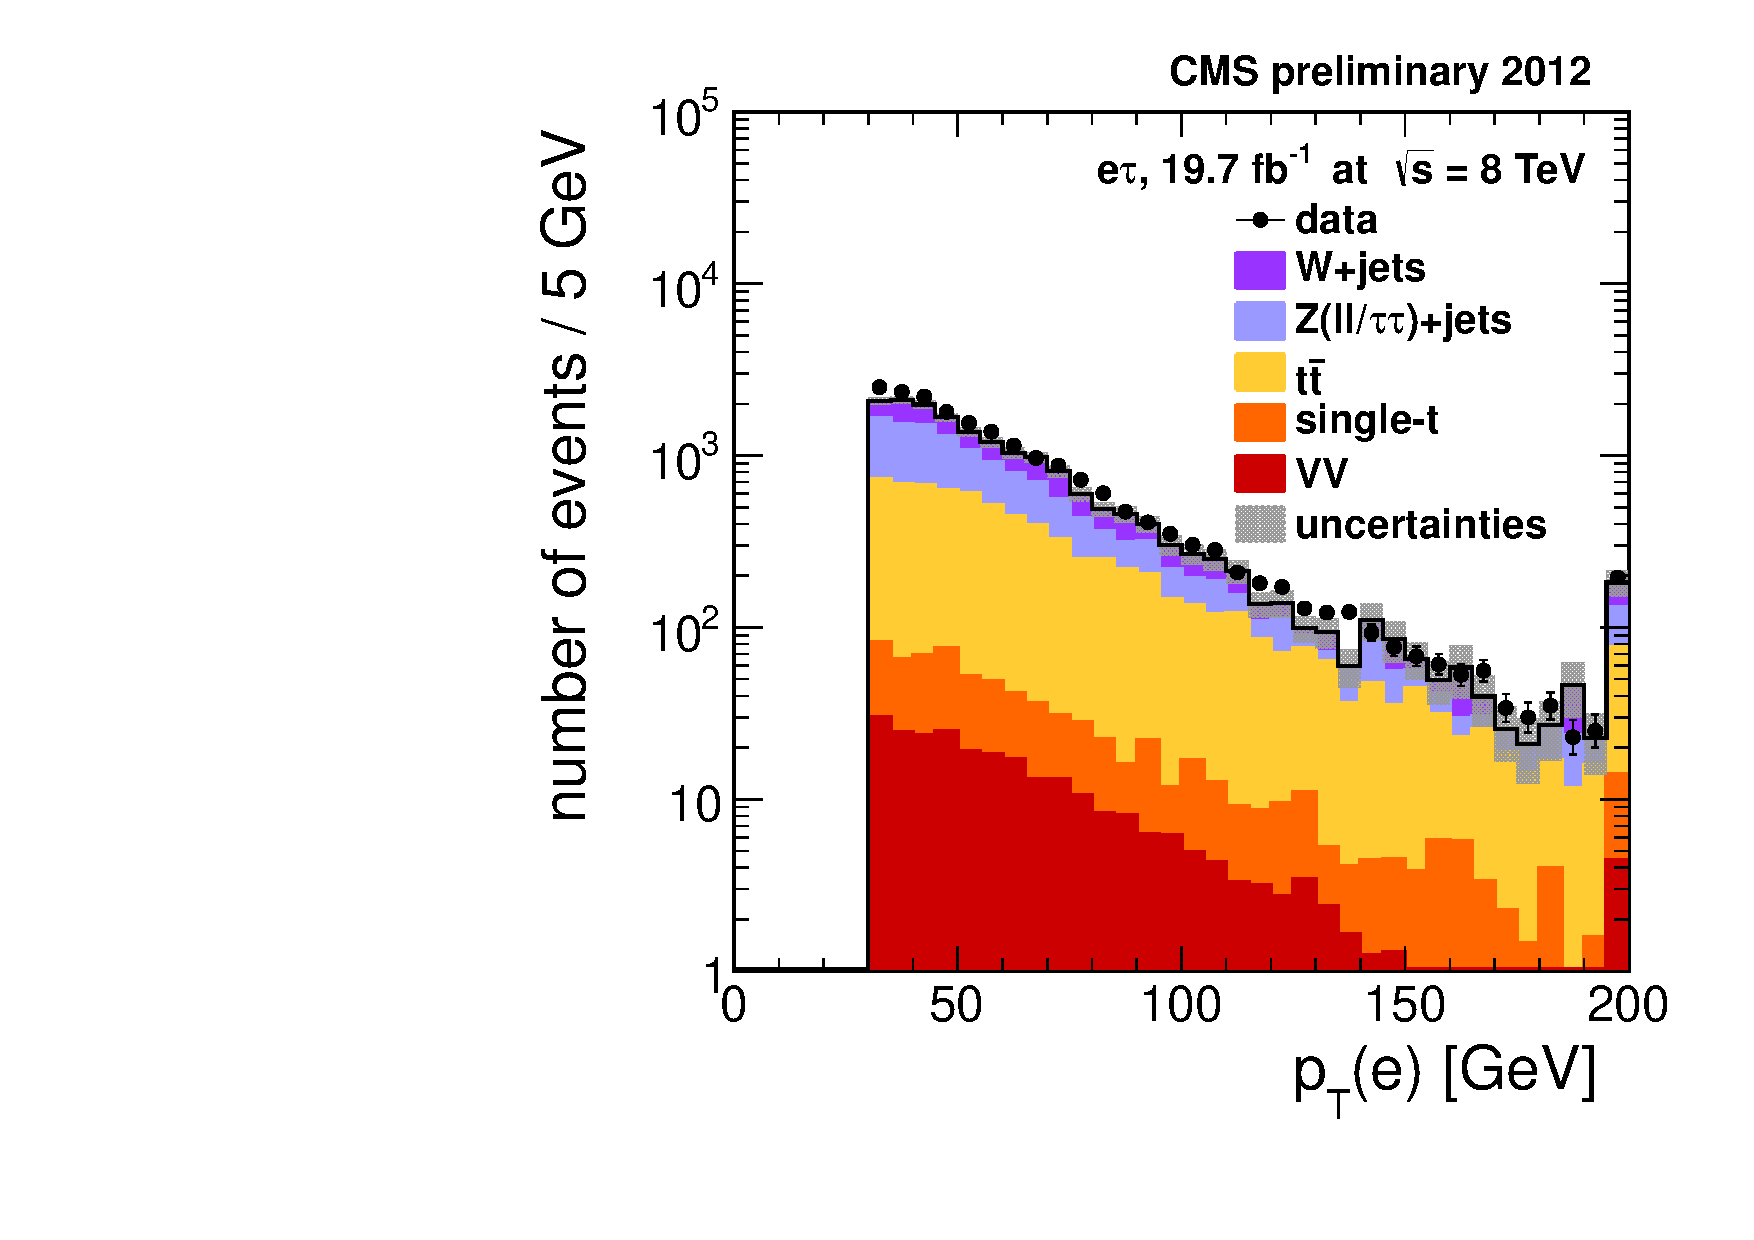
\includegraphics[width=0.465\textwidth]{figures/etau/elPtMultJet.pdf}
    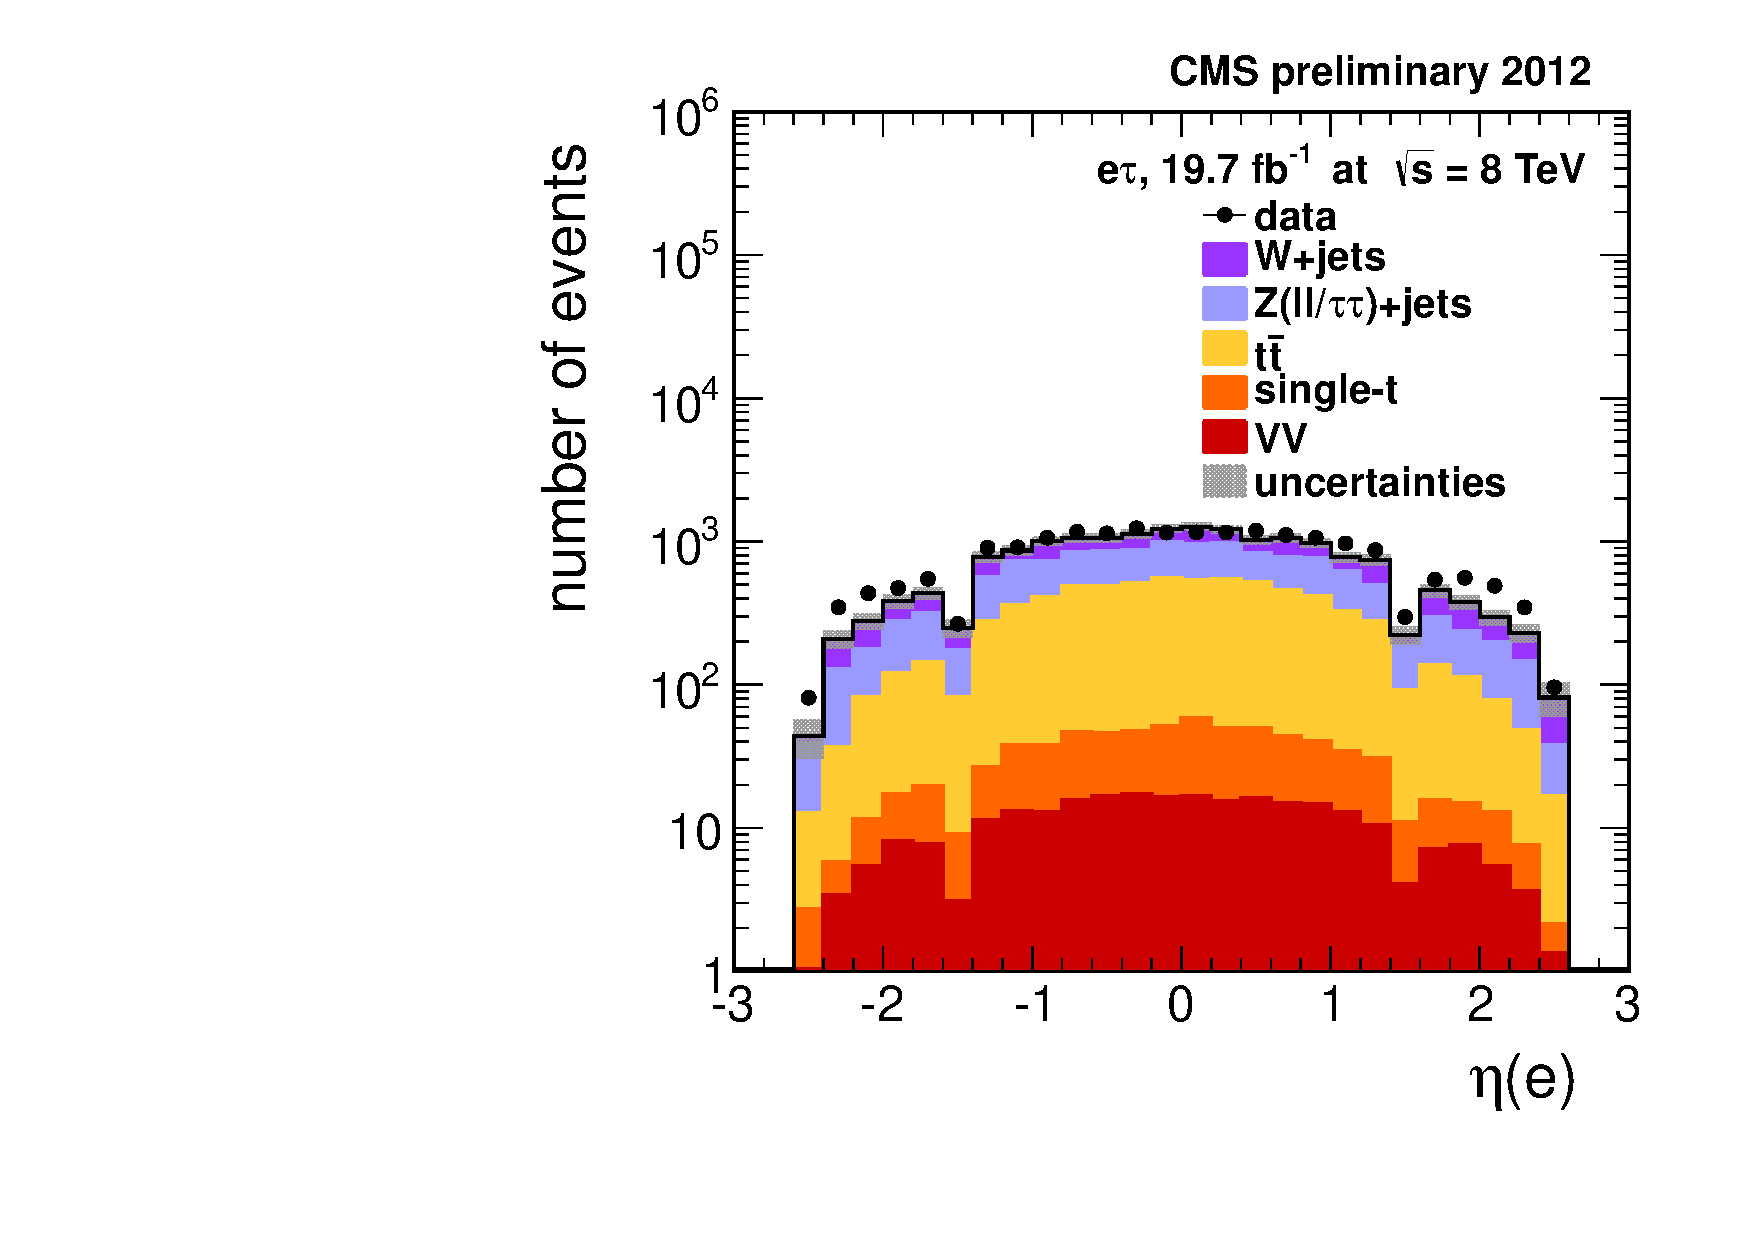
\includegraphics[width=0.465\textwidth]{figures/etau/elEtaMultJet.pdf} \\
    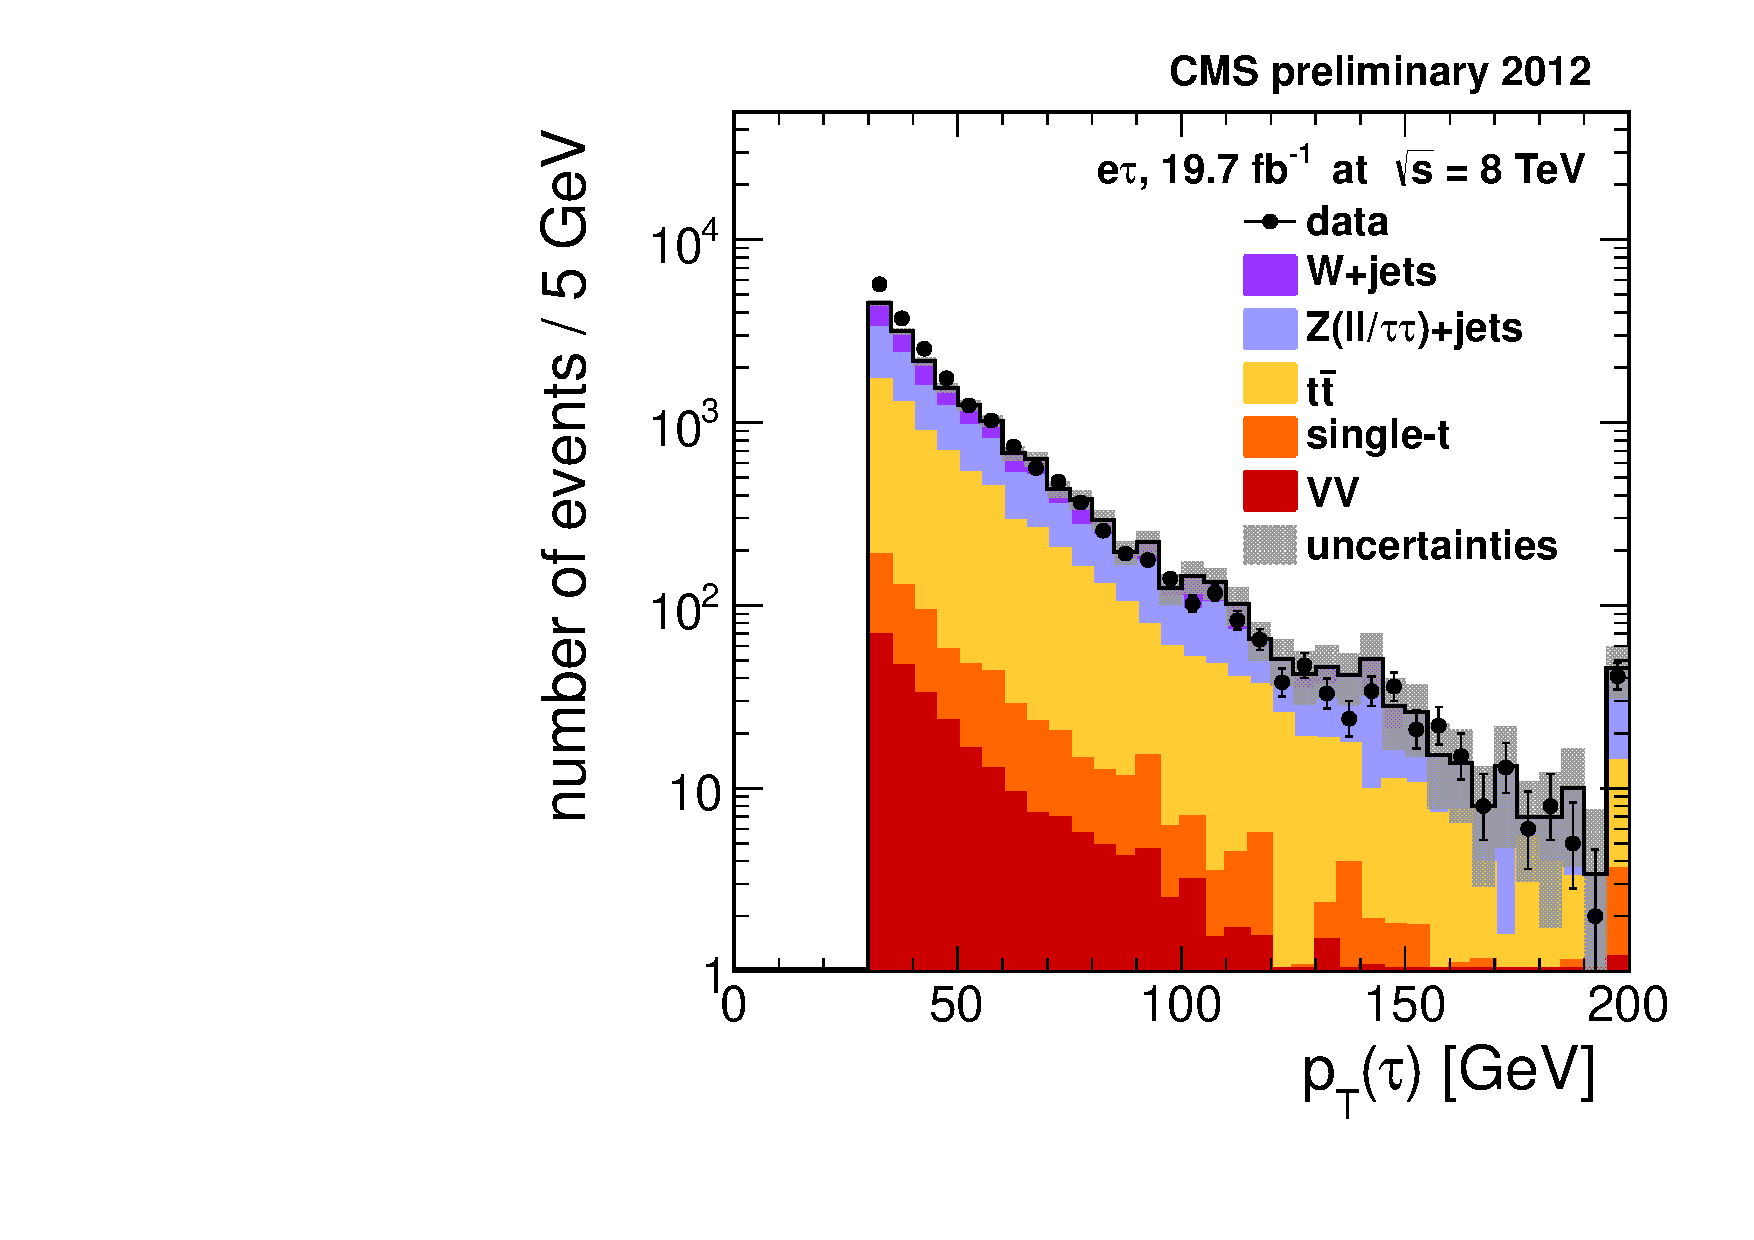
\includegraphics[width=0.465\textwidth]{figures/etau/tauPtMultJet.pdf}
    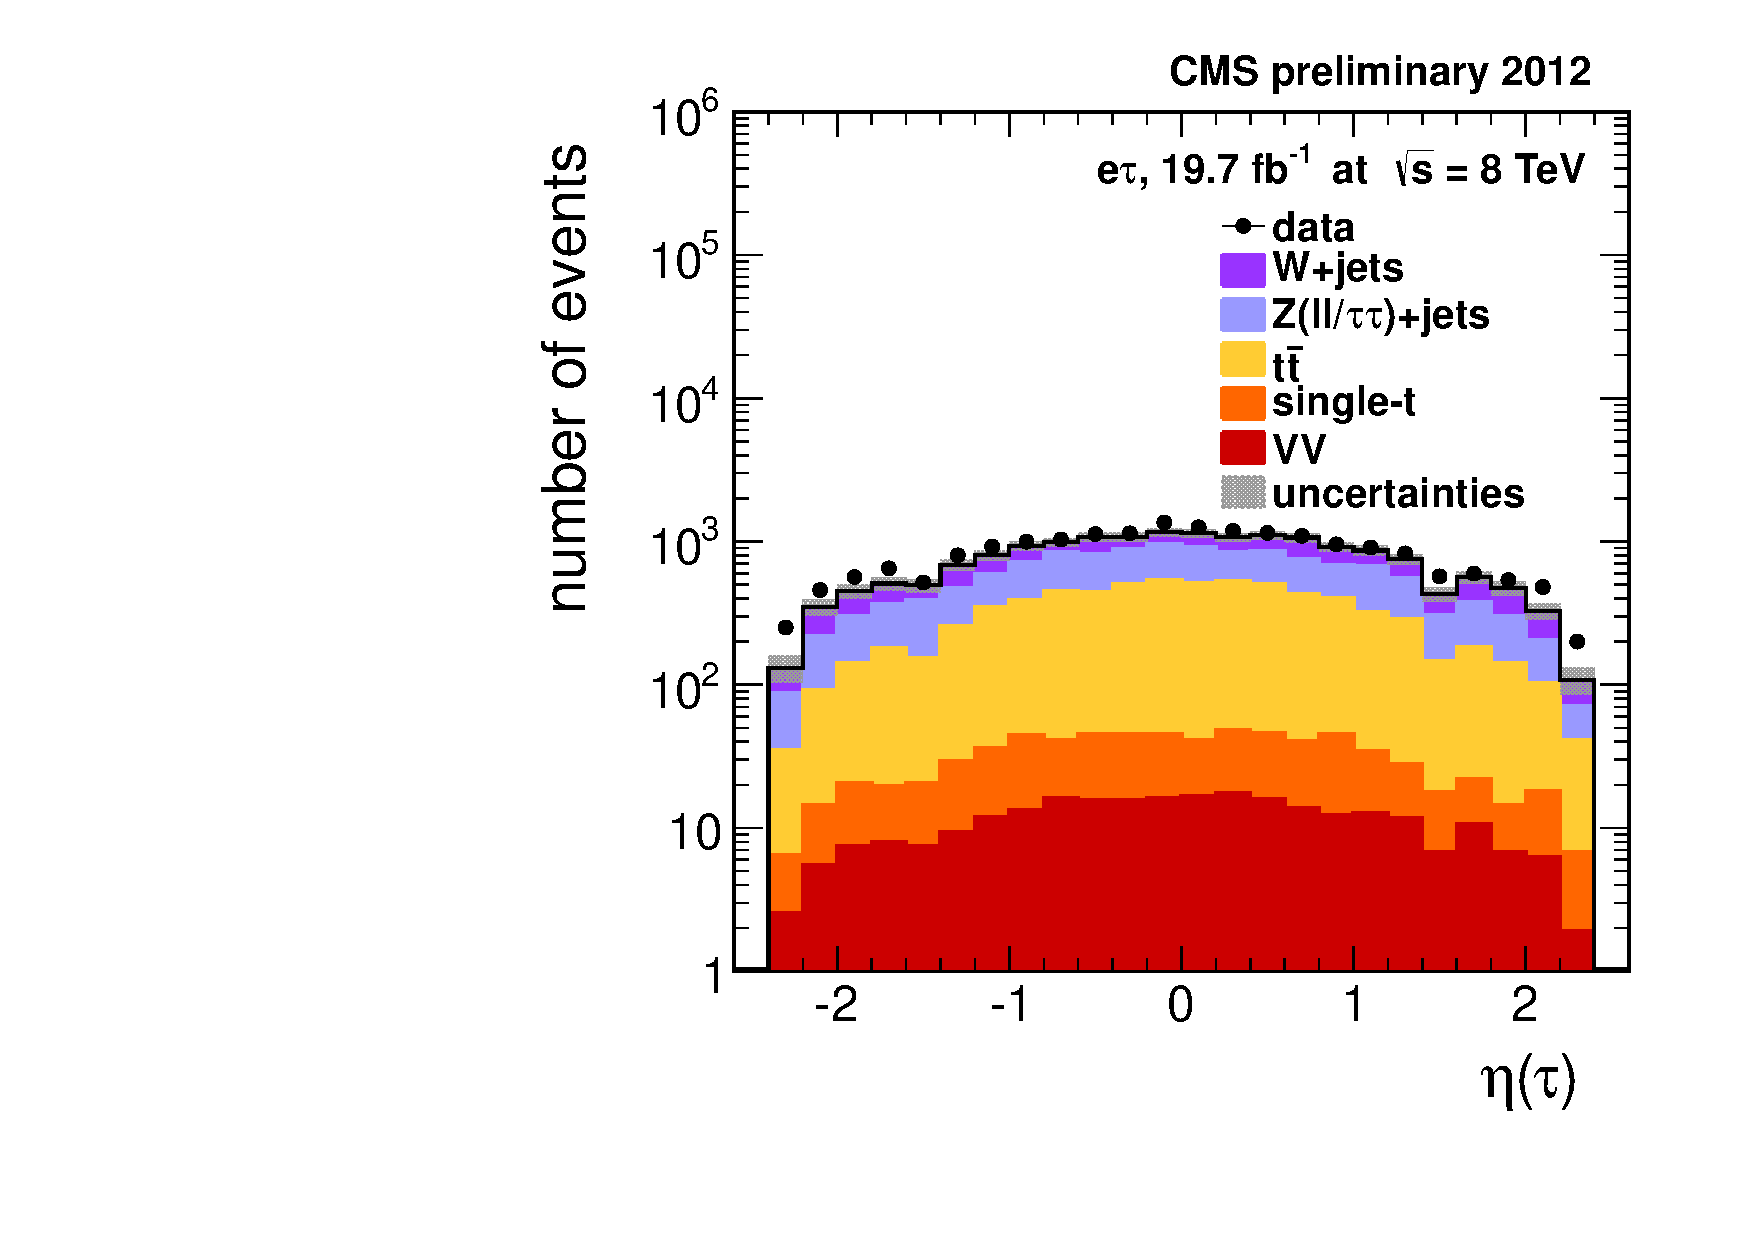
\includegraphics[width=0.465\textwidth]{figures/etau/tauEtaMultJet.pdf}
    \caption{Plots of various kinematic quantities comparing observed data and simulated backgrounds in the \etau channel after the preselection: the visible mass of the electron and hadronic tau (top left), the number of b-tagged jets (top right), the \pt (left) and $\eta$ (right) of the electron (middle) and hadronic tau (bottom). The uncertainty band reflects the statistical uncertainty in the simulated backgrounds.}
    \label{fig:preseletau}
  \end{center}
\end{figure}

\begin{figure}[hbtp]
  \begin{center}
    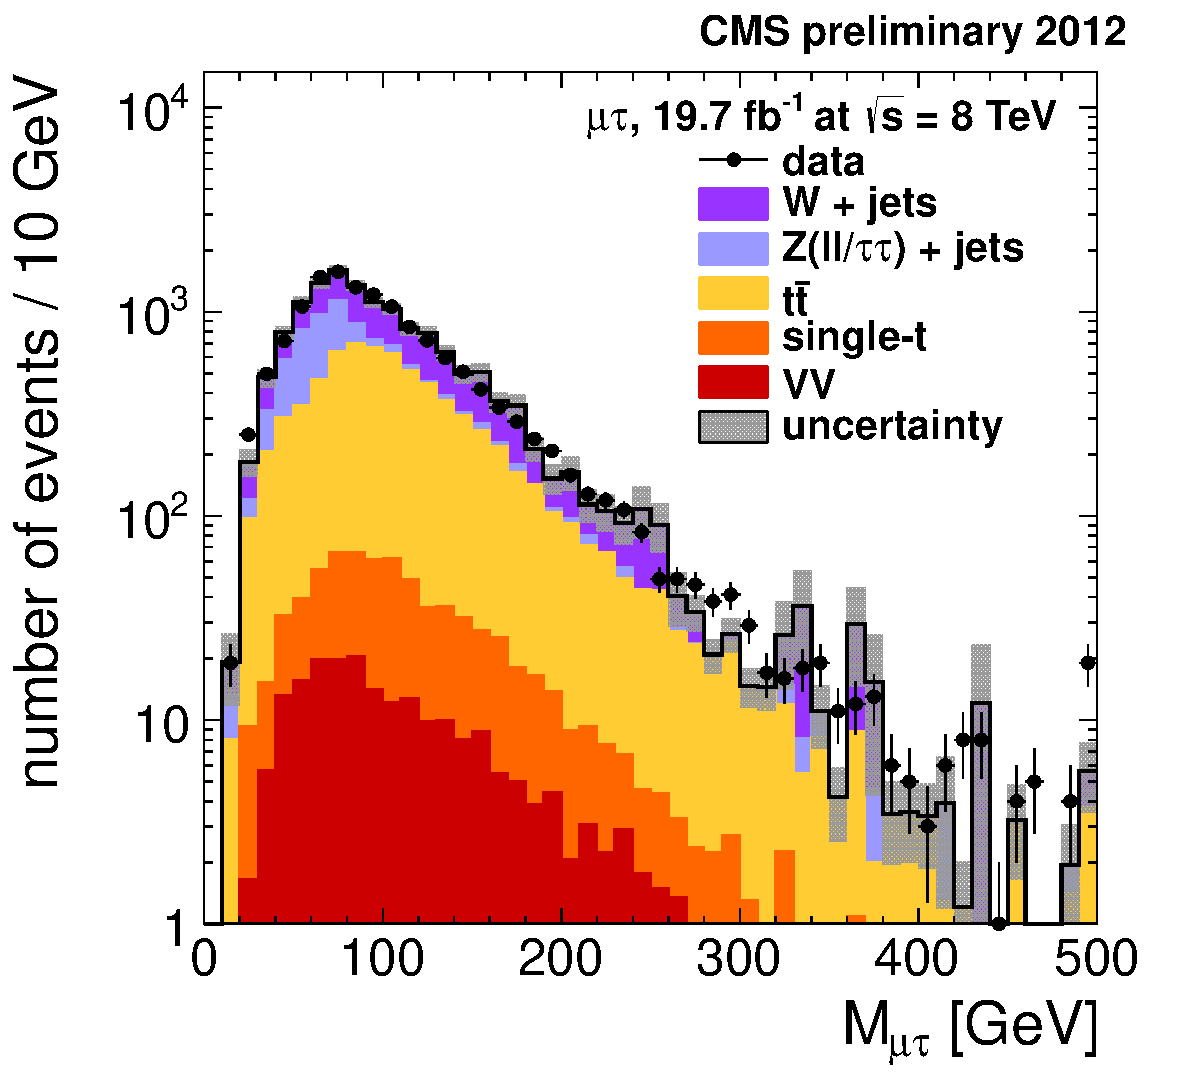
\includegraphics[width=0.465\textwidth]{figures/mutau/preselection/mass.pdf}
    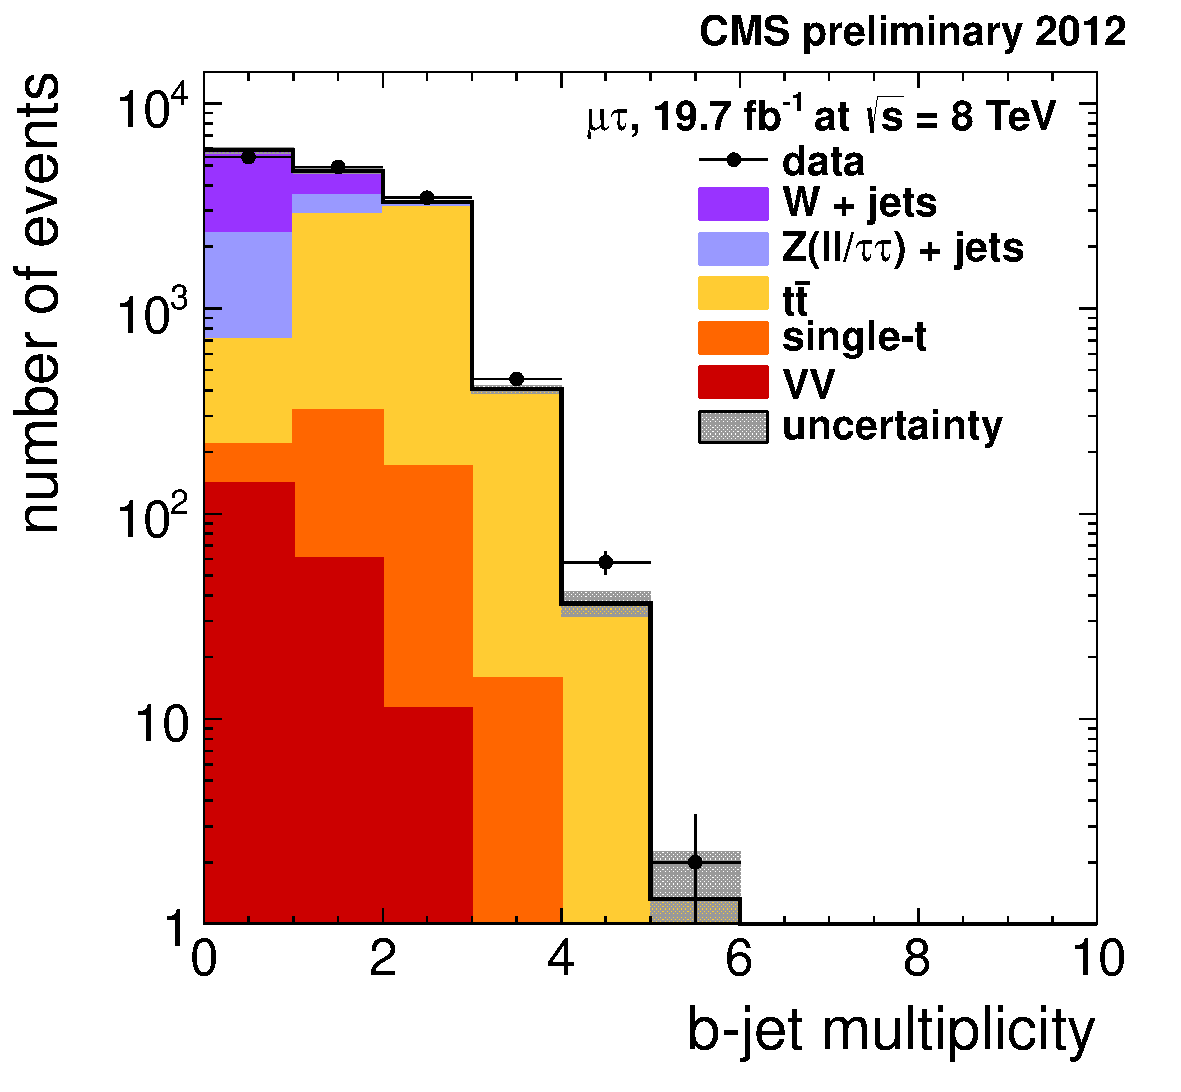
\includegraphics[width=0.465\textwidth]{figures/mutau/preselection/nbjet.pdf} \\
    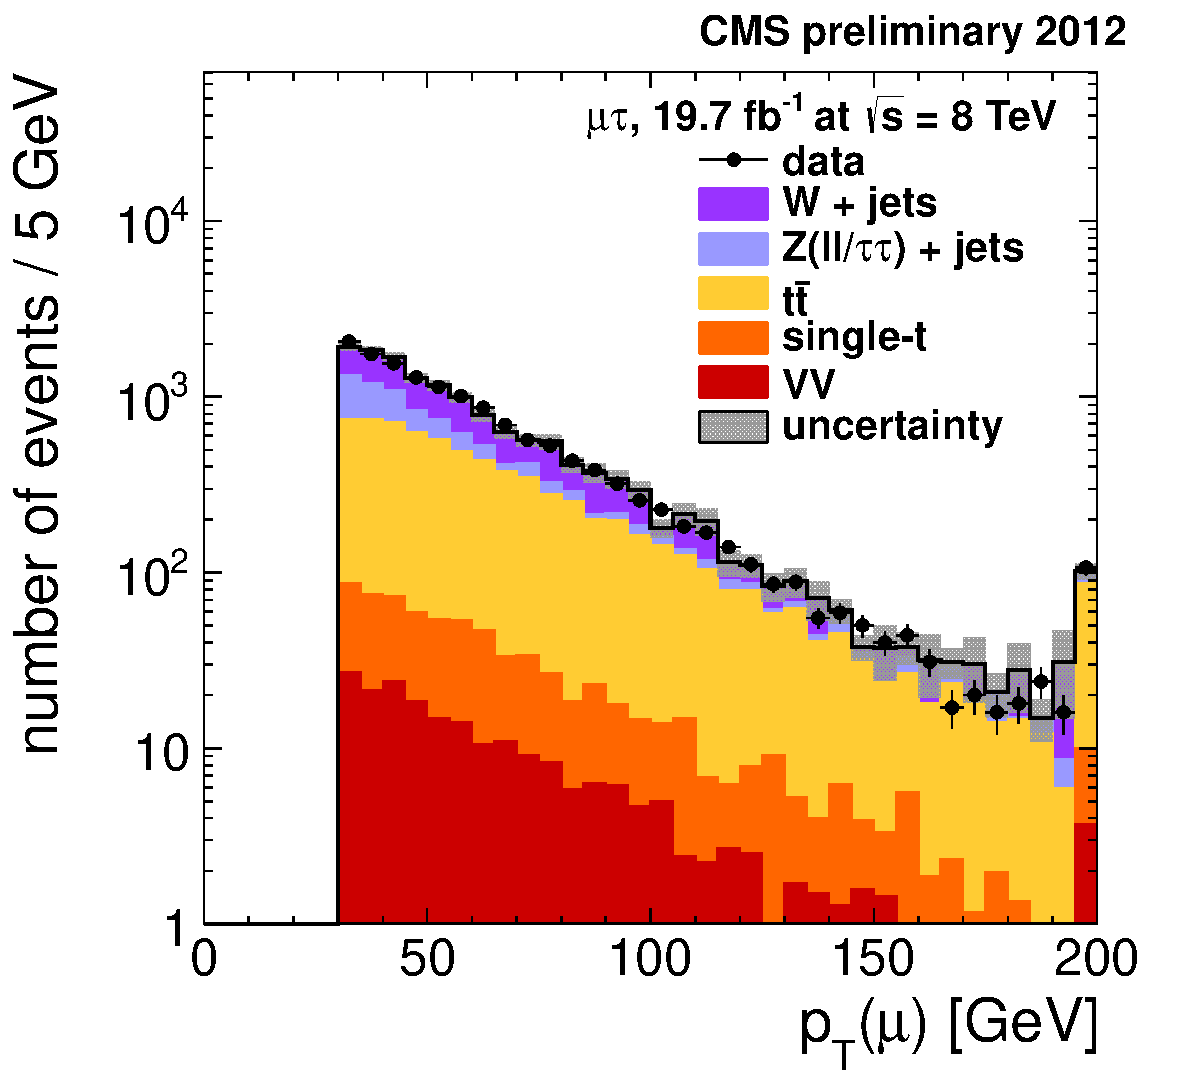
\includegraphics[width=0.465\textwidth]{figures/mutau/preselection/ptmu.pdf}
    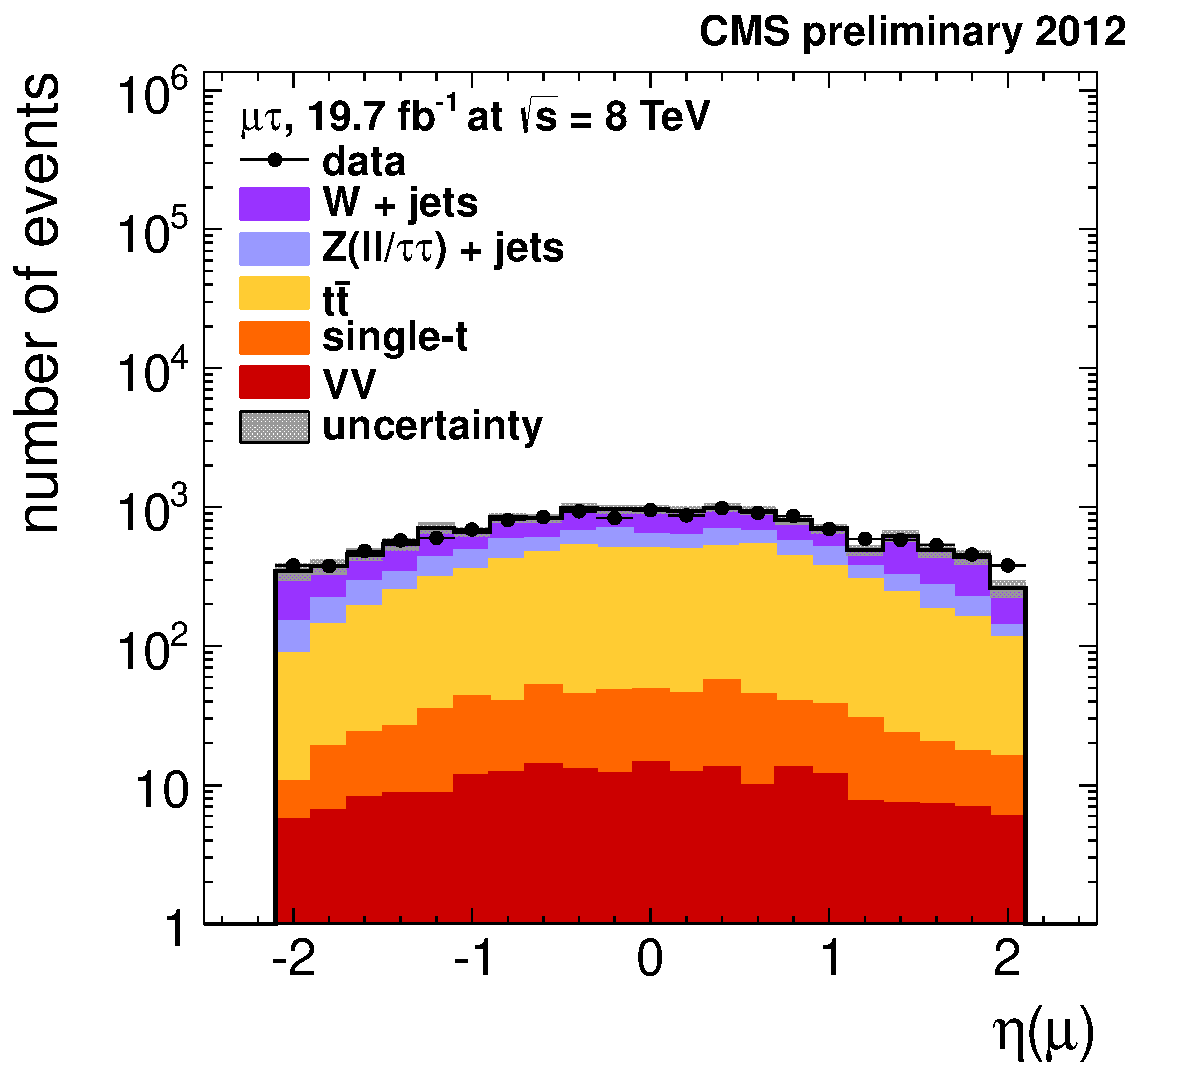
\includegraphics[width=0.465\textwidth]{figures/mutau/preselection/etamu.pdf} \\
    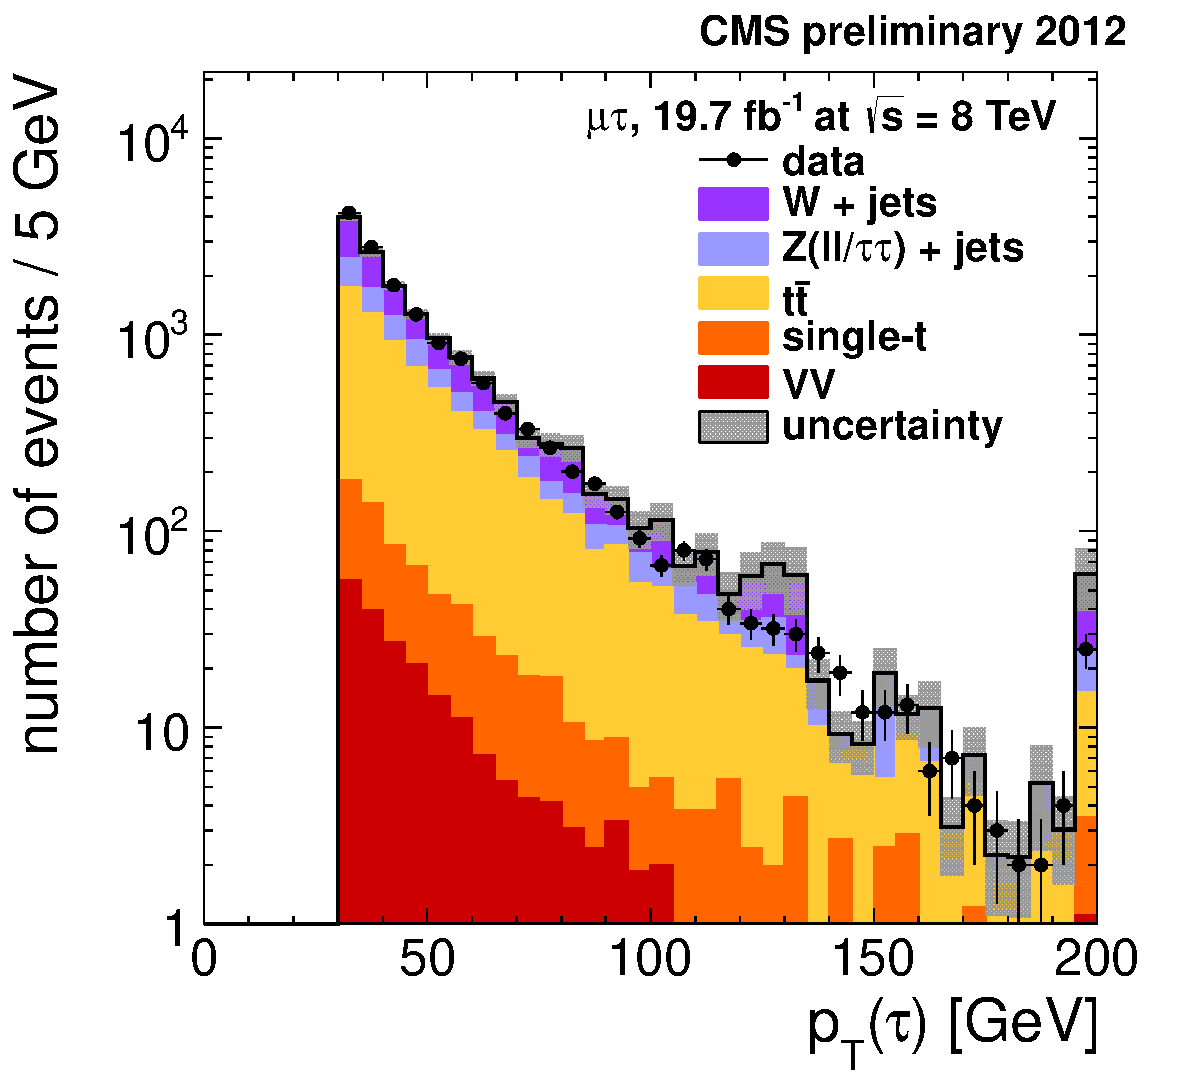
\includegraphics[width=0.465\textwidth]{figures/mutau/preselection/pttau.pdf}
    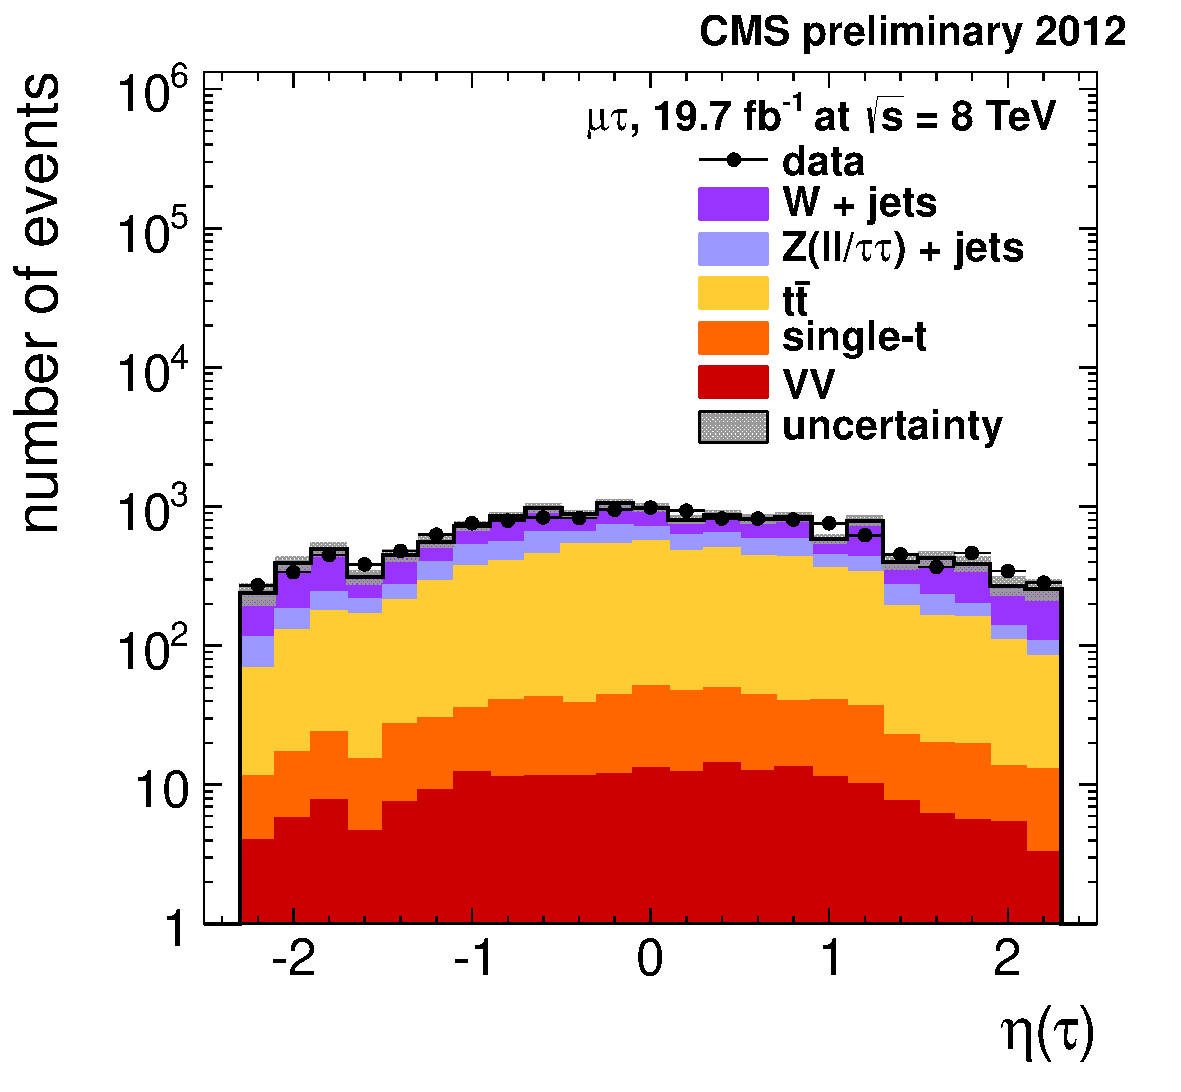
\includegraphics[width=0.465\textwidth]{figures/mutau/preselection/etatau.pdf}
    \caption{Plots of various kinematic quantities comparing observed data and simulated backgrounds in the \mutau channel after the preselection: the visible mass of the muon and hadronic tau (top left), the number of b-tagged jets (top right), the \pt (left) and $\eta$ (right) of the muon (middle) and hadronic tau (bottom). The uncertainty band reflects the statistical uncertainty in the simulated backgrounds.}
    \label{fig:preselmutau}
  \end{center}
\end{figure}

\begin{table}[hbt]
  \begin{center}
    \begin{tabular}{|l|r@{$\,\pm\,$}r|r@{$\,\pm\,$}r|}
      \hline
      & \multicolumn{2}{c|}{\etau channel} & \multicolumn{2}{c|}{\mutau channel} \\
      \hline
      \W + jets                       &  4221.6 & 188.1   & 4846.3 & 233.6  \\
      \Z + jets                       &  4766.7 & 85.1    & 2369.1 & 80.7   \\
      \ttbar                          &  6272.2 & 65.5    & 6430.5 & 69.8   \\
      Single \cPqt                    &  462.9 & 14.4     & 512.3 & 16.0    \\
      VV                              &  223.4 & 4.4      & 212.5 & 4.6     \\
      QCD multijets                   &  (2452.6 & 512.1)\neghphantom{)} & \multicolumn{2}{c|}{---} \\ 
      \hline                                                  
      Total Bkg. (no QCD)             & 15946.8 & 232.9   & 14370.8 & 257.3 \\
      \hline                                                  
      \hline                                                  
      Data                            & \multicolumn{1}{r@{\hphantom{$\,\pm\,$}}}{18177\hphantom{.0}} & & \multicolumn{1}{r@{\hphantom{$\,\pm\,$}}}{14351\hphantom{.0}} & \\
      \hline
    \end{tabular}
    \caption{The simulated background and observed event yields after the preselection in the \etau and \mutau channels. The statistical uncertainties are given for each simulated background. The contribution from the QCD multijets process is not taken into account in the total background yield. }
    \label{tab:eventyieldpresel}
  \end{center}
\end{table}

%\clearpage

\subsection{Main Selection}

A preselected event satisfies the main selection if at least one of the selected jets in the event is b-tagged. Though the expected final state from the signal includes two b-jets, it was found that requiring b-tagging for only one jet improved the signal yield in comparison to the SM backgrounds. This is expected due to the reduced efficiency of applying the CSV algorithm for b-tagging multiple times per event. The second jet in the event may or may not be b-tagged. Plots comparing observed data to the simulated backgrounds after the main selection are shown in Figs. \ref{fig:mainseletau} and \ref{fig:mainselmutau}, and event yields are given in Table \ref{tab:eventyieldmainsel}.

At this stage of the selection, several new observables are introduced. The first is the visible mass of the hadronic tau and a jet, \MassTJ. There are two possible pairings of the light lepton and the hadronic tau with the two selected jets. The pairing is chosen to minimize the difference between \MassTJ and \MassLJ. In signal events, these two values are expected to be similar, as both sets of correctly-paired particles will originate from the same mother particles, leptoquarks or top squarks. However, the visible mass variables will not directly measure the true mass of the mother particles; some of the energy will be lost in the form of neutrinos produced in tau lepton decays. According to the simulation of the signal process, this minimization selects the correct pairing in approximately 70\% of events. This observable will be used in the final selection for the leptoquark search.

The second new variable is \ST, which is defined as the scalar sum of \pt for all final-state objects:
\begin{equation}
\label{eq:STLQ}
\ST(\text{LQ}) = \pt(\ell) + \pt(\tauh) + \pt(\text{b-jet}) + \pt(\text{jet}).
\end{equation}
As indicated in Eq. \eqref{eq:STLQ}, this definition of \ST is appropriate for the leptoquark search, which requires four objects in the final state: a light lepton, a hadronic tau, a b-tagged jet, and another jet. Figures \ref{fig:mainseletau} and \ref{fig:mainselmutau} show this version of \ST. An alternate definition appropriate for the top squark search, which has a slightly different final state, is given in Eq. \eqref{eq:STstop}.

\begin{figure}[hbtp]
  \begin{center}
    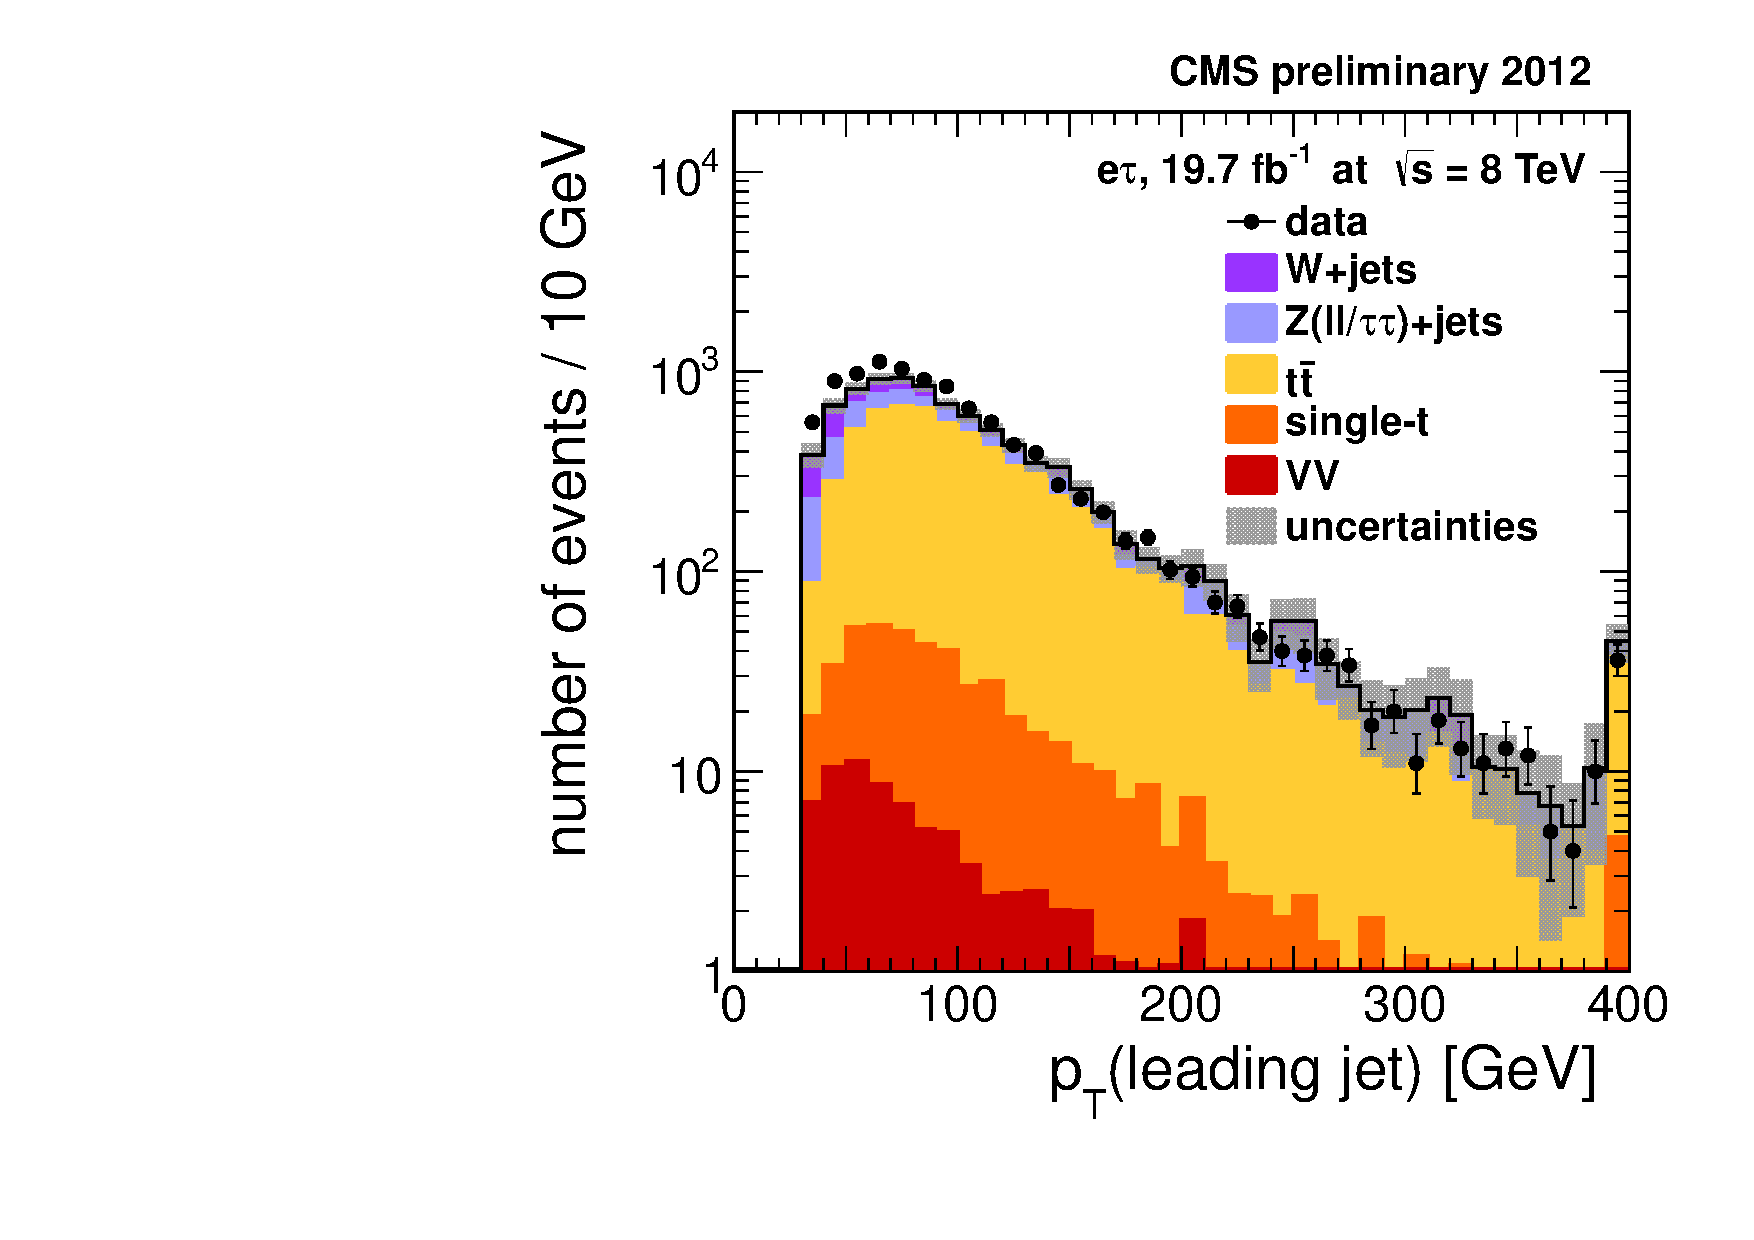
\includegraphics[width=0.49\textwidth]{figures/etau/jet1PtBTag.pdf}
    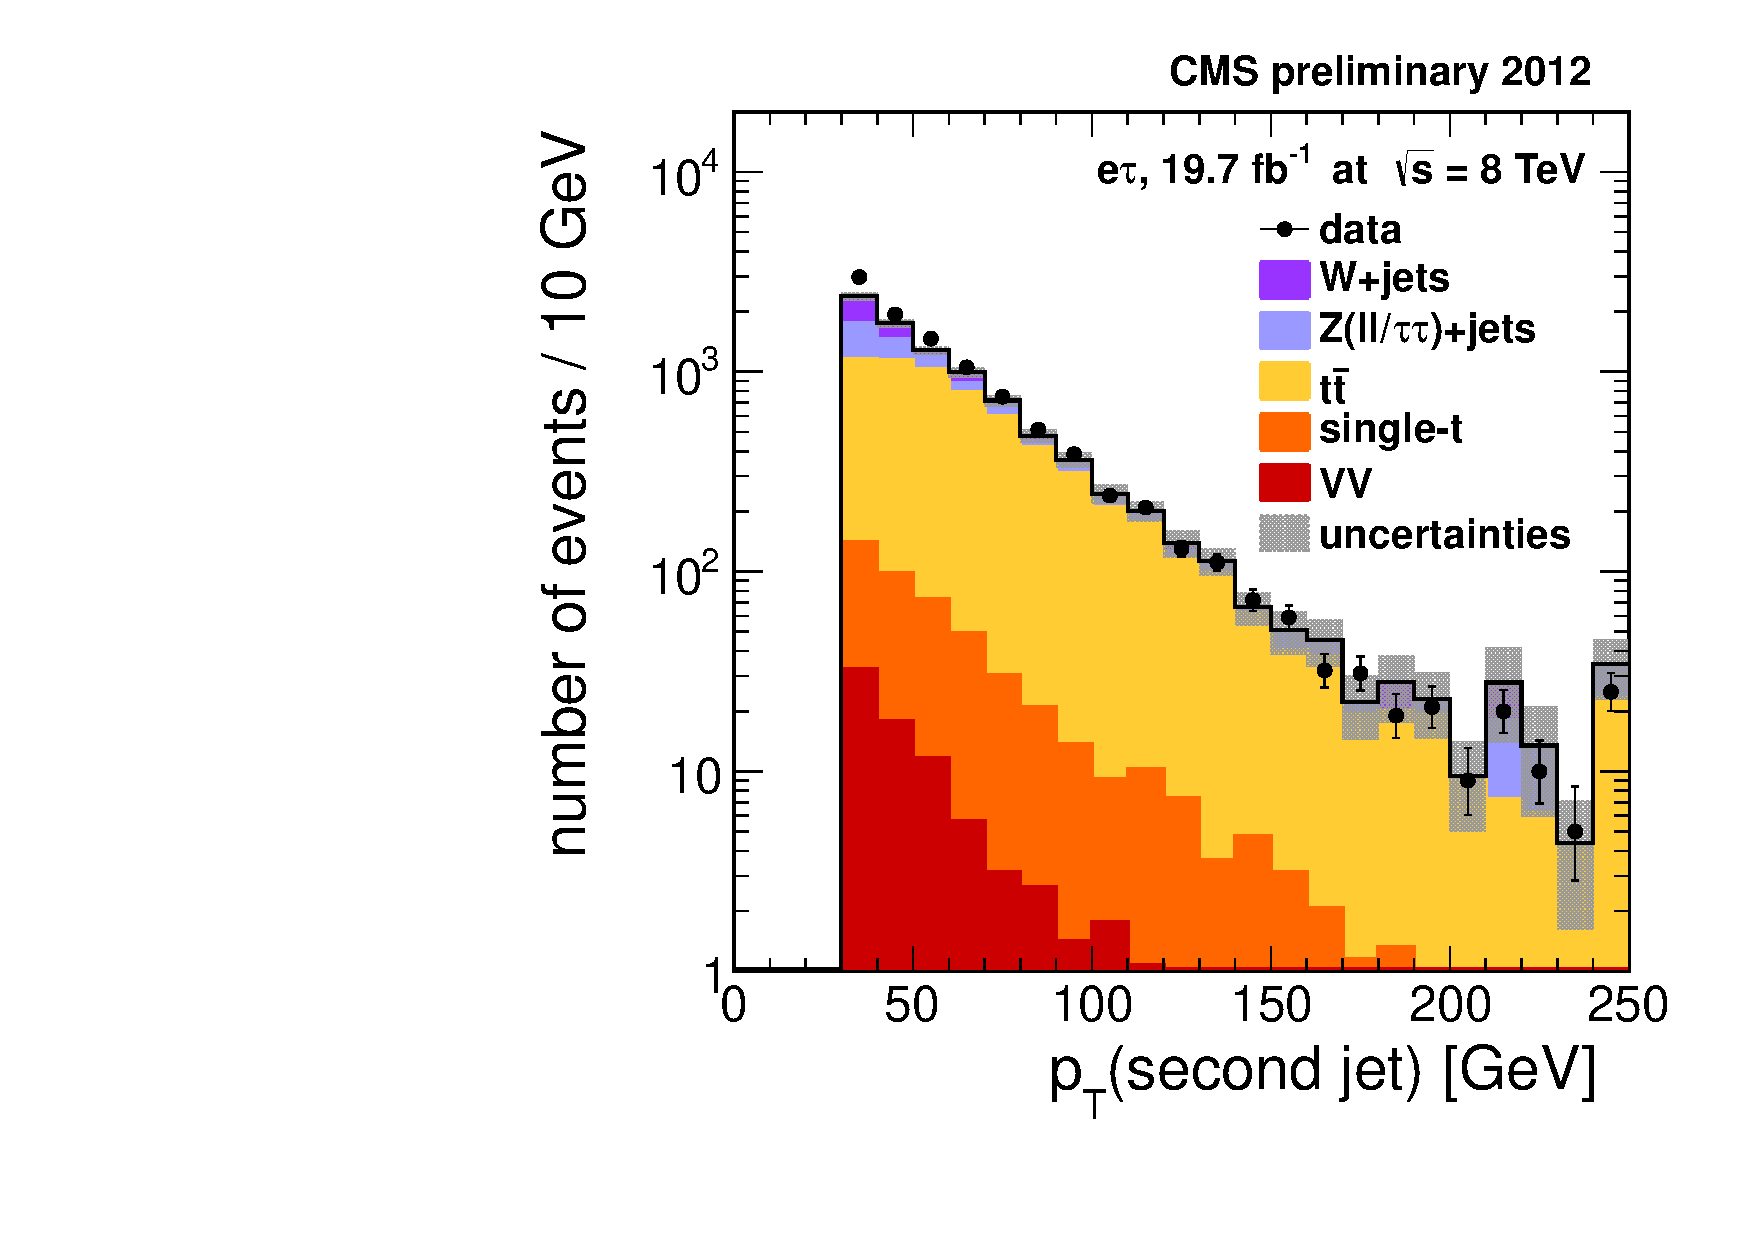
\includegraphics[width=0.49\textwidth]{figures/etau/jet2PtBTag.pdf} \\
    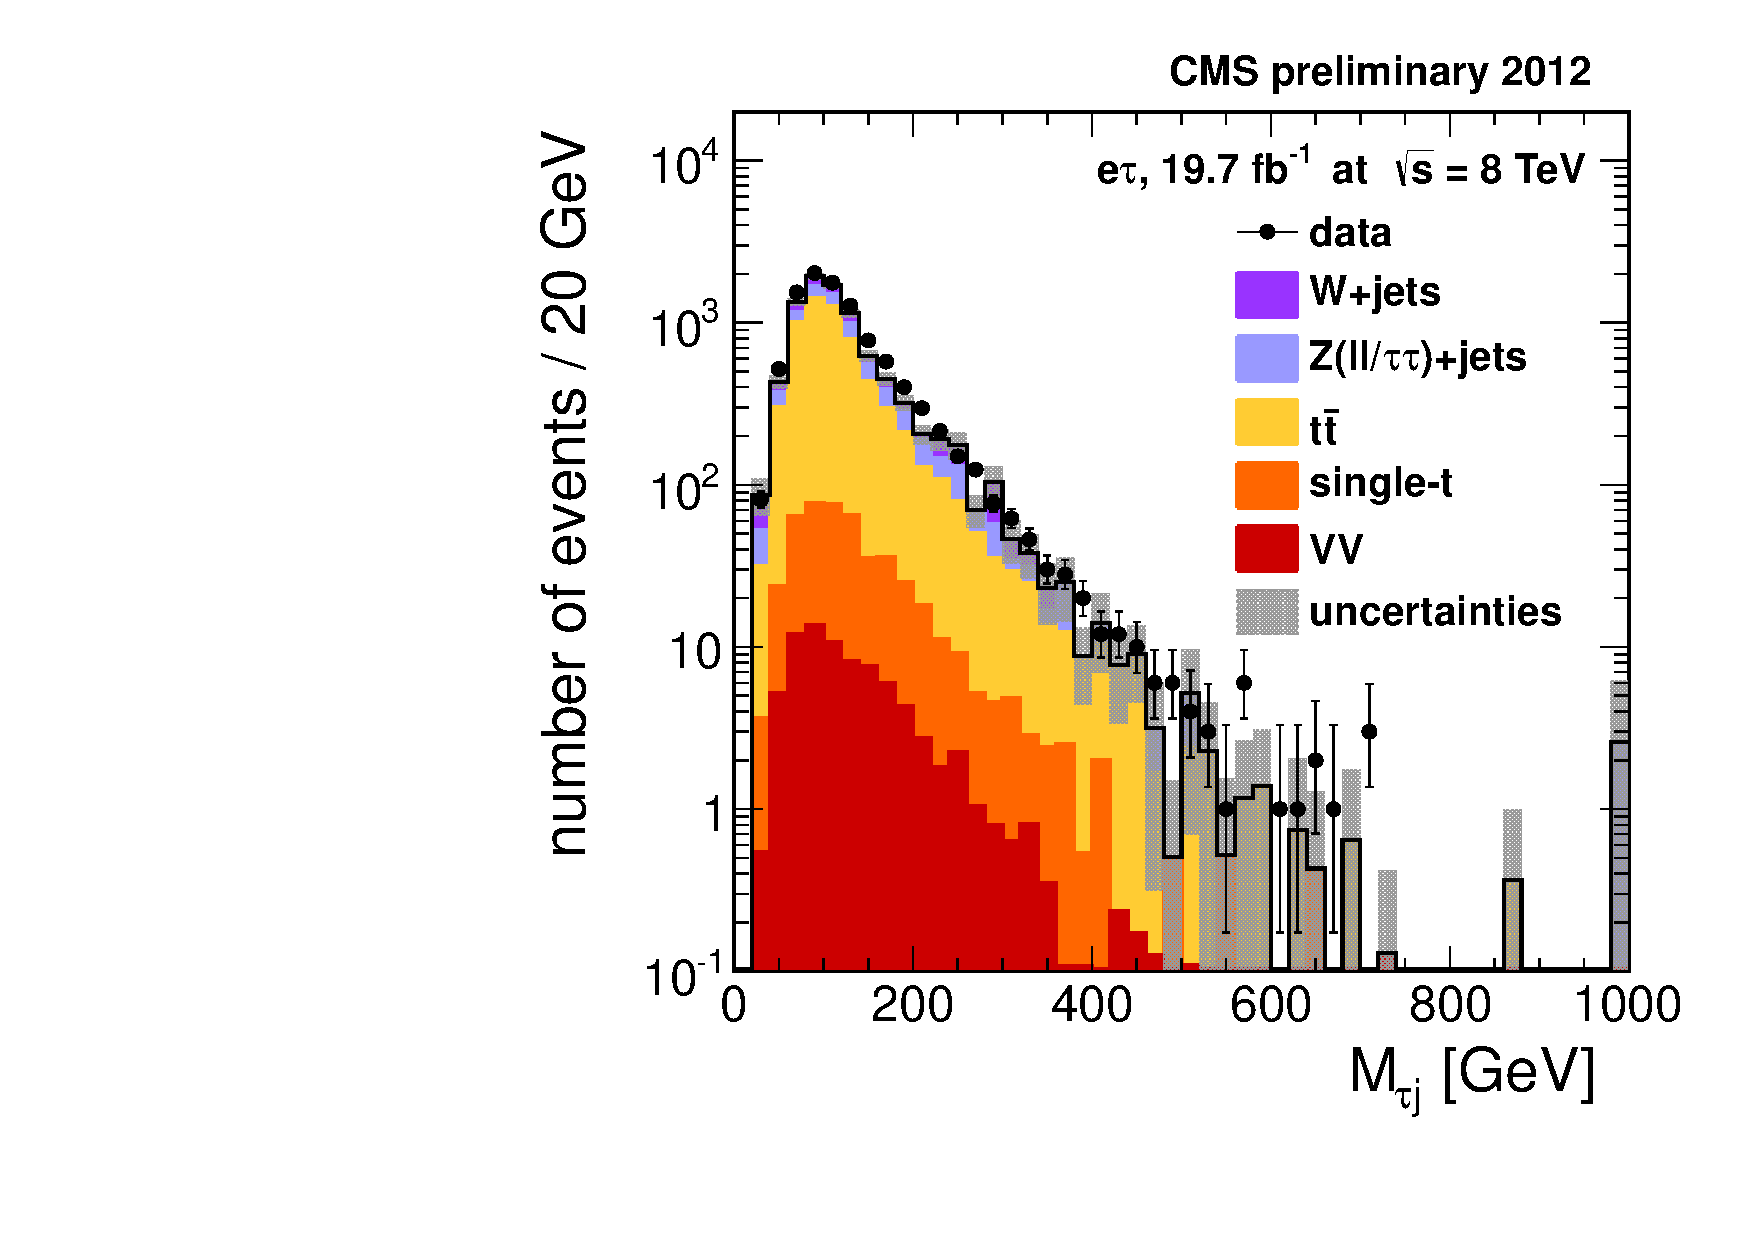
\includegraphics[width=0.49\textwidth]{figures/etau/finalMass.pdf}
    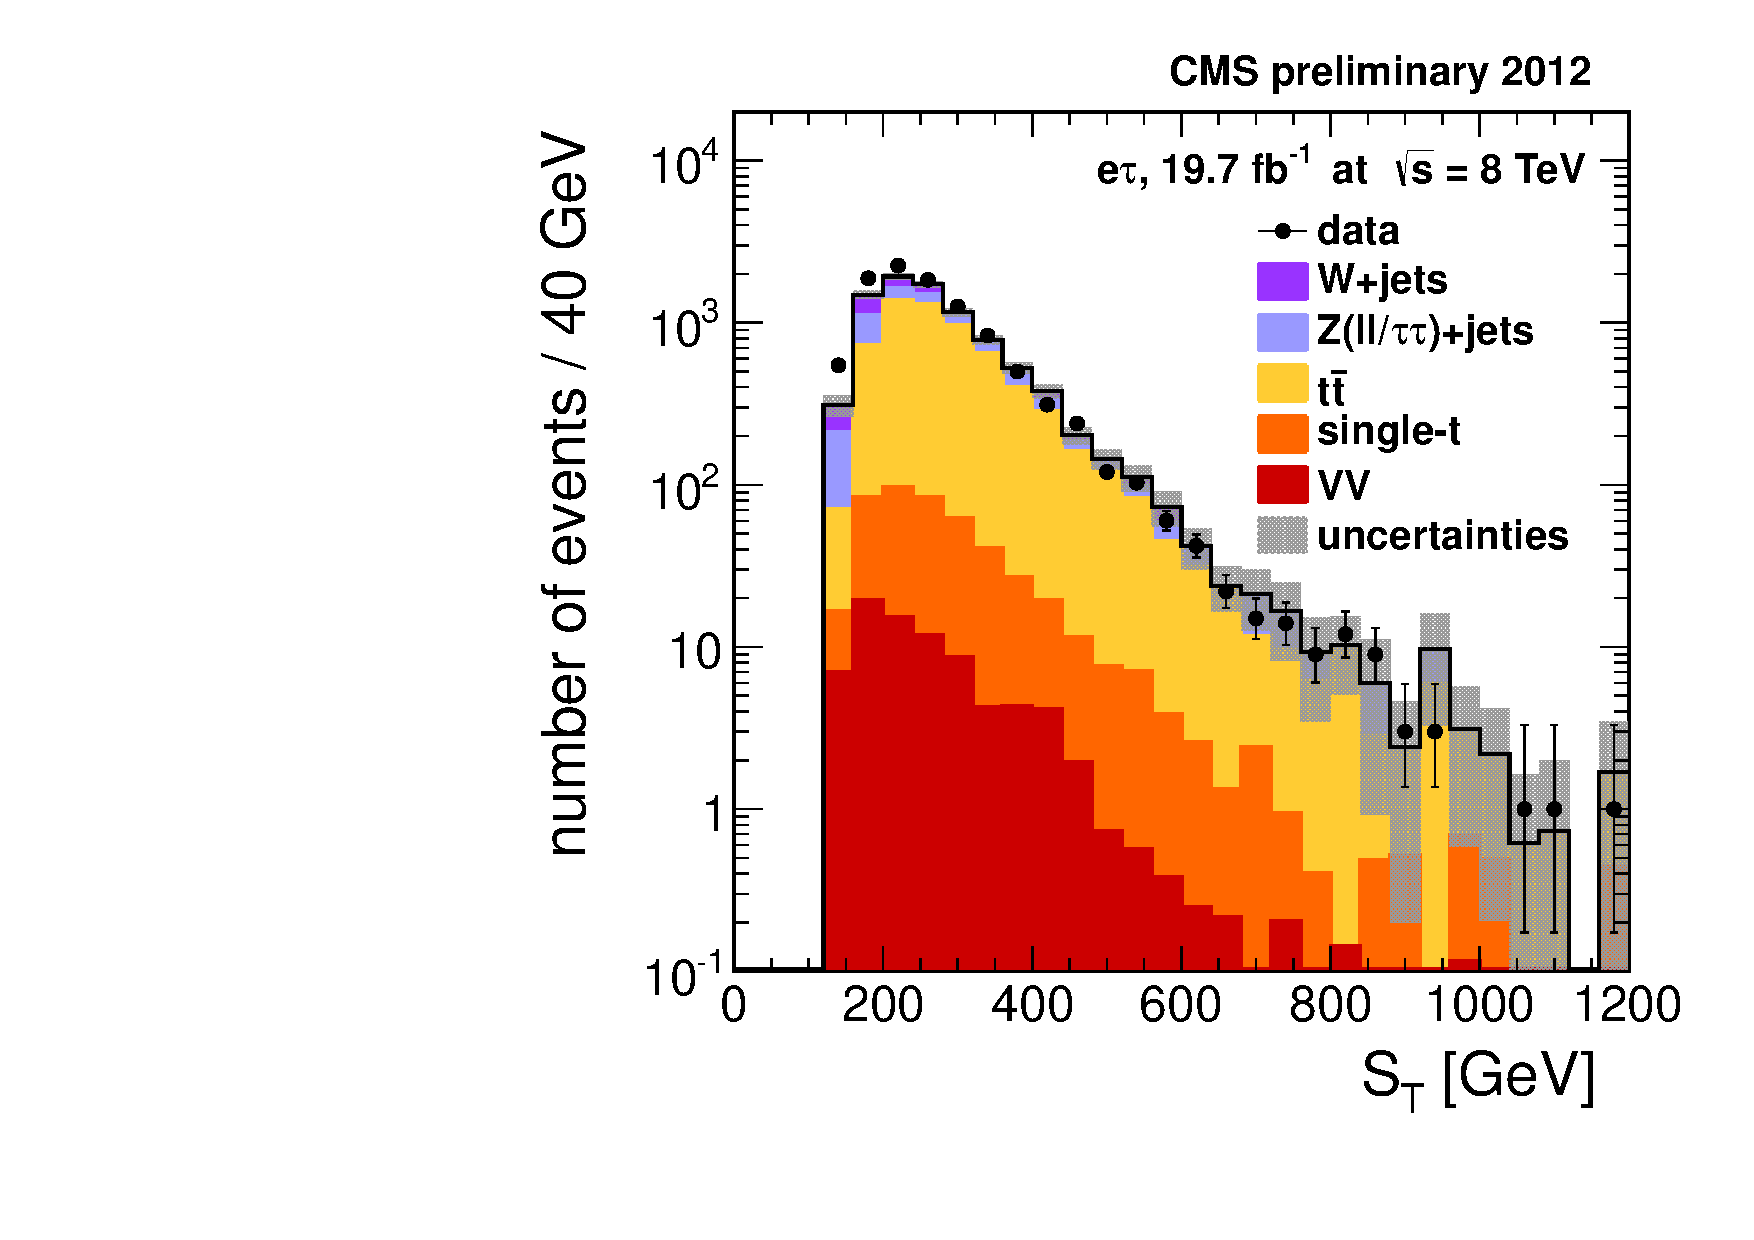
\includegraphics[width=0.49\textwidth]{figures/etau/STbjetBTag.pdf}
    \caption{Plots of various kinematic quantities comparing observed data and simulated backgrounds in the \etau channel after the main selection: the \pt spectra (top) of the first (left) and second (right) selected jets, \MassTJ (bottom left), and \ST (bottom right). The uncertainty band reflects the statistical uncertainty in the simulated backgrounds.}
    \label{fig:mainseletau}
  \end{center}
\end{figure}

\begin{figure}[hbtp]
  \begin{center}
    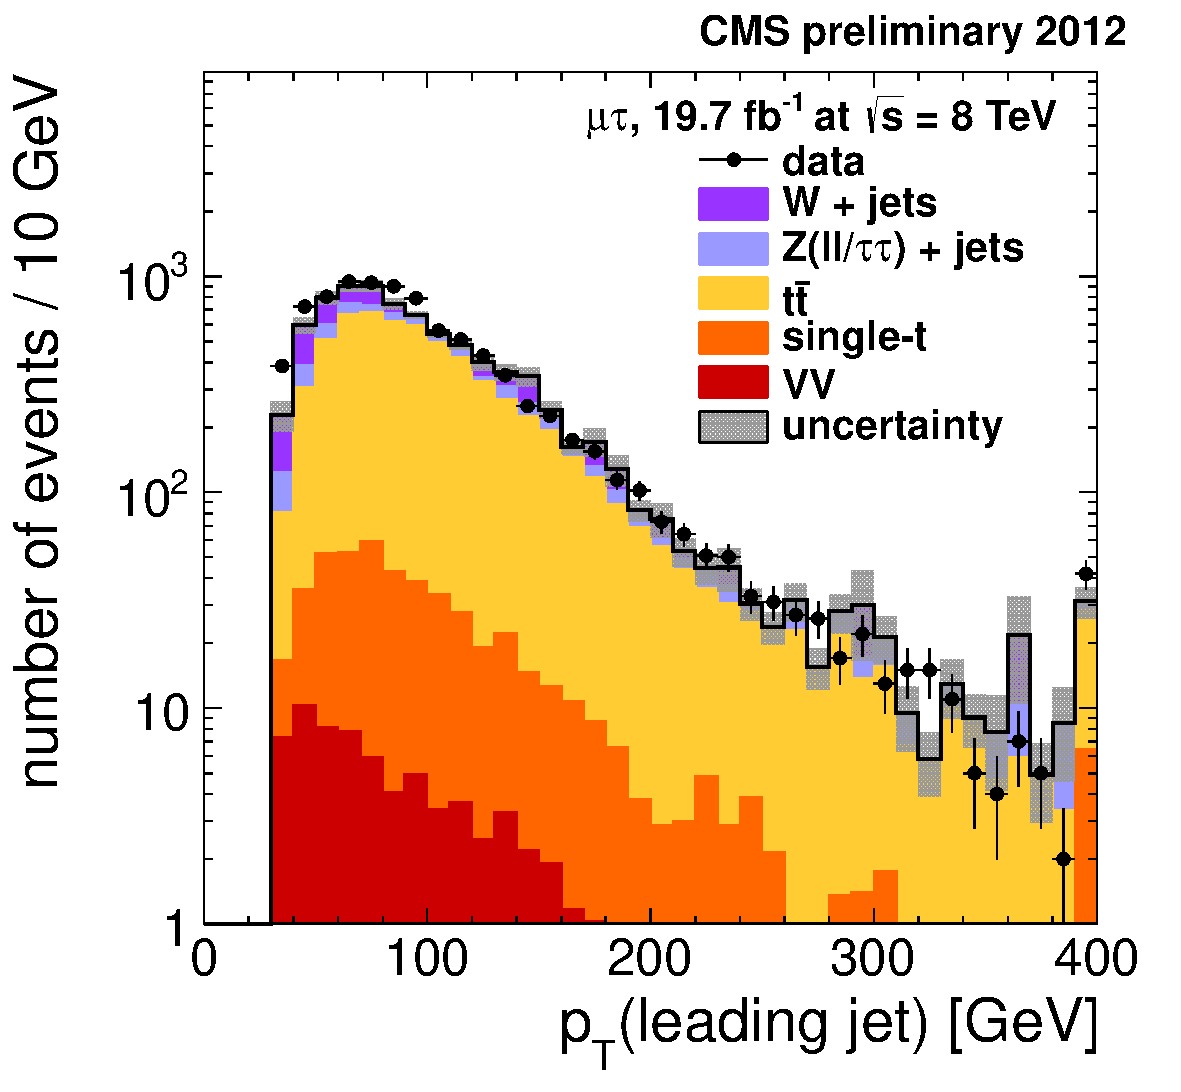
\includegraphics[width=0.49\textwidth]{figures/mutau/mainselection/leadseljetpt.pdf}
    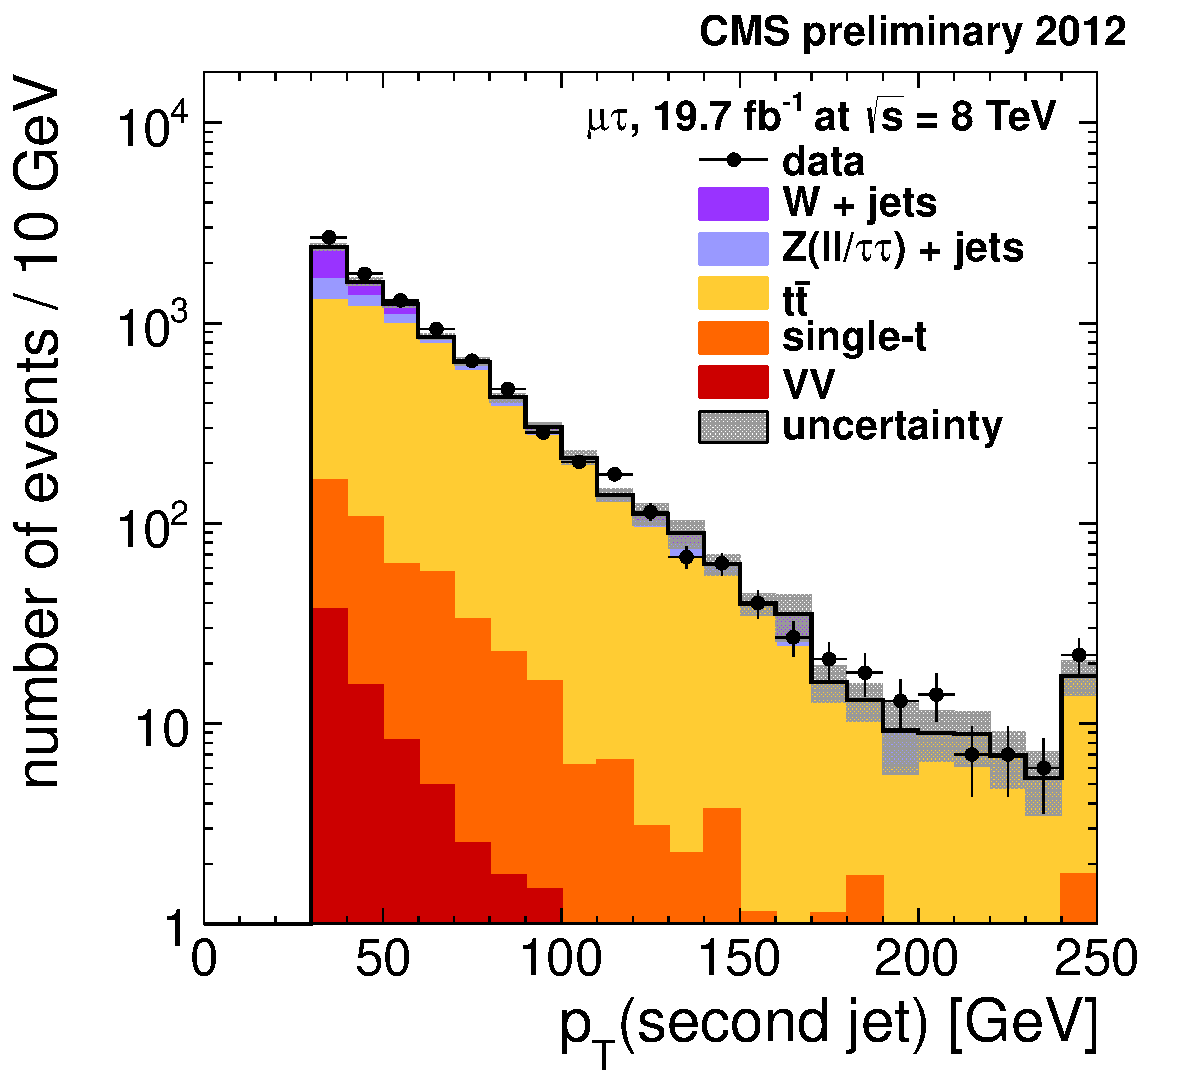
\includegraphics[width=0.49\textwidth]{figures/mutau/mainselection/secondseljetpt.pdf} \\
    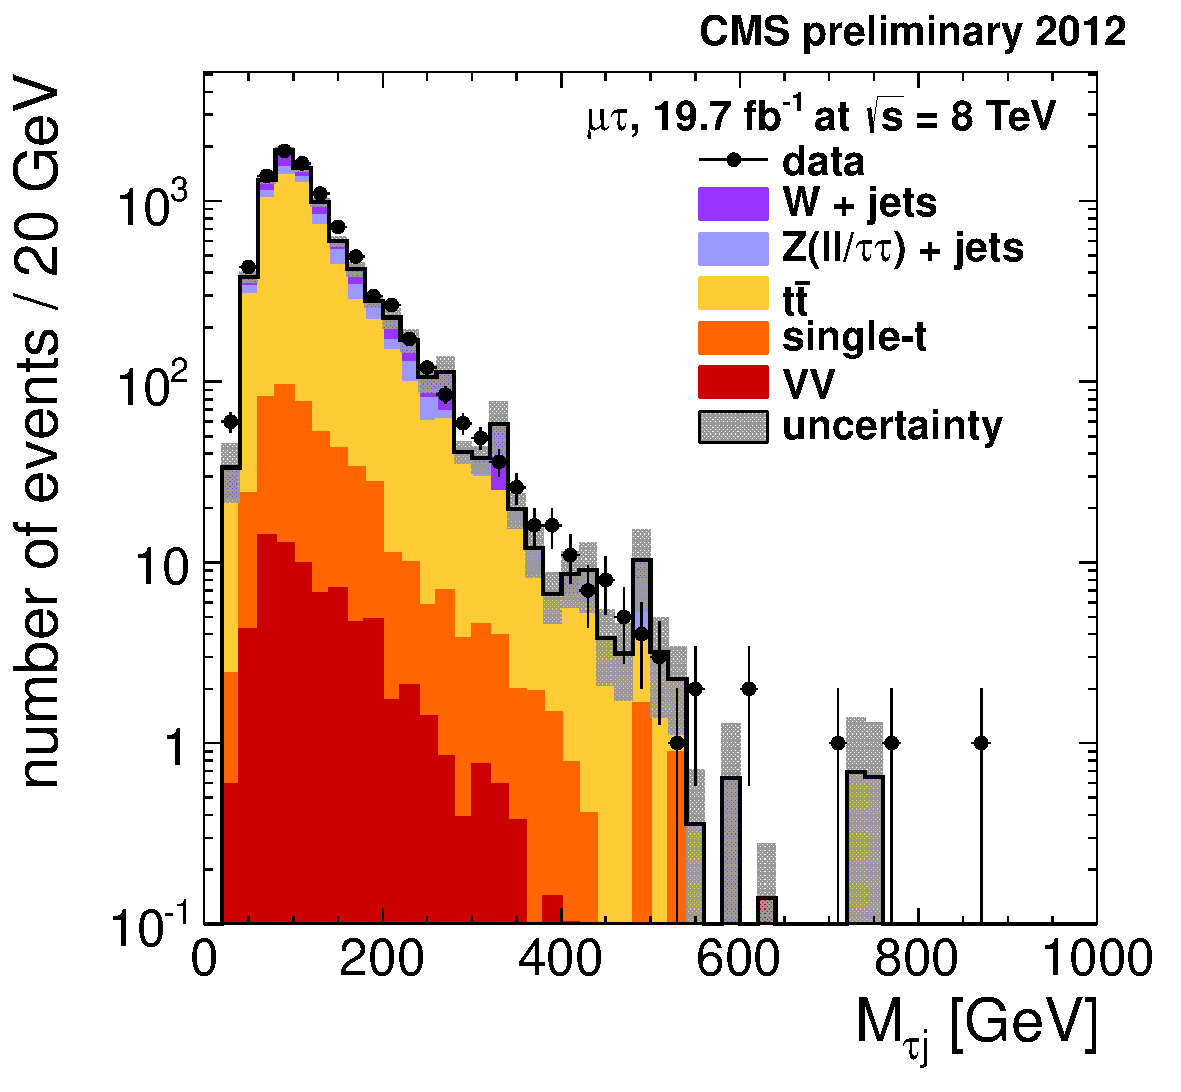
\includegraphics[width=0.49\textwidth]{figures/mutau/mainselection/masstaub.pdf}    
    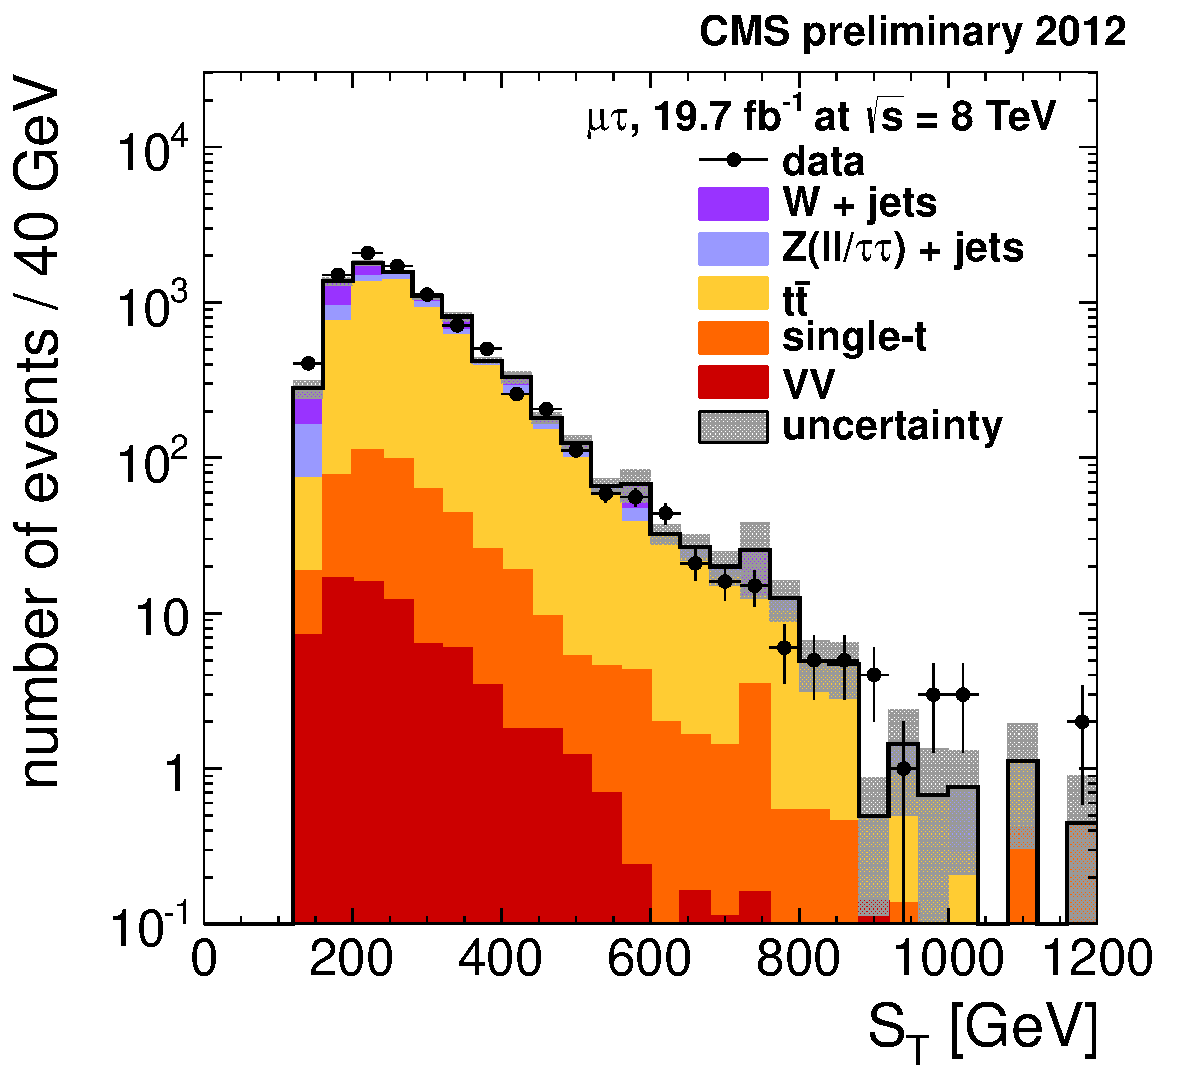
\includegraphics[width=0.49\textwidth]{figures/mutau/mainselection/st.pdf}
    \caption{Plots of various kinematic quantities comparing observed data and simulated backgrounds in the \mutau channel after the main selection: the \pt spectra (top) of the first (left) and second (right) selected jets, \MassTJ (bottom left), and \ST (bottom right). The uncertainty band reflects the statistical uncertainty in the simulated backgrounds.}
    \label{fig:mainselmutau}
  \end{center}
\end{figure}

\begin{table}[hbt]
  \begin{center}
    \begin{tabular}{|l|r@{$\,\pm\,$}r|r@{$\,\pm\,$}r|}
      \hline
      & \multicolumn{2}{c|}{\etau channel} & \multicolumn{2}{c|}{\mutau channel} \\
      \hline
      \W + jets                       & 1201.9 & 104.0   & 1285.8 & 122.7 \\
      \Z + jets                       & 1534.0 & 49.5    & 774.4 & 46.8   \\
      \ttbar                          & 5783.6 & 63.5    & 5699.5 & 64.4  \\
      Single \cPqt                    & 390.2  & 13.5    & 418.6 & 14.2   \\
      VV                              & 82.9   & 2.7     & 74.1 & 2.7     \\
      QCD multijets                   & (1226.0 & 131.0)\neghphantom{)}  & \multicolumn{2}{c|}{---}  \\
      \hline                                                 
      Total Bkg. (no QCD)             & 8992.6 & 141.2   & 8252.3 & 147.0 \\
      \hline
      \hline
      Data                            & \multicolumn{1}{r@{\hphantom{$\,\pm\,$}}}{10113\hphantom{.0}} & & \multicolumn{1}{r@{\hphantom{$\,\pm\,$}}}{8866\hphantom{.0}} &  \\
      \hline
    \end{tabular}
    \caption{The simulated background and observed event yields after the main selection in the \etau and \mutau channels. The statistical uncertainties are given for each simulated background. The contribution from the QCD multijets process is not taken into account in the total background yield. }
    \label{tab:eventyieldmainsel}
  \end{center}
\end{table}

%\clearpage

\subsection{Final Selections}

In the final stage of the selection for the leptoquark search, two additional requirements are applied. The selected hadronic tau must have $\pt>50\GeV$, and the selected events must have $\MassTJ>250\GeV$. This cut on the \MassTJ value is optimal for the expected limit based on the simulation for the entire range of leptoquark masses under consideration. The change in the kinematic properties of the signal for different mass values is taken into account when the \ST distribution is used to set $\text{CL}_{s}$ limits. The procedure for setting limits with a distribution is described in App. \ref{ch:limits}.

Slightly different final selection criteria are applied for the top squark search. Again, the selected hadronic tau must have $\pt>50\GeV$. Instead of a cut on \MassTJ, which is not a meaningful variable for the top squark $\lambda^{\prime}_{3jk}$ decay chain, the selected events are required to have $N_{\text{jets}}\geq5$. The expected final state of the top squark signal has $N_{\text{jet}}=6$, and though it was found that requiring $N_{\text{jets}}\geq6$ would maximize the expected limit based on the simulation, the number of both signal and background events passing that cut was greatly reduced. Because this would also reduce the number of events in the control regions used to estimate the major backgrounds, the corresponding increase in systematic uncertainty would render the limit indistinguishable from the $N_{\text{jets}}\geq5$ case. Thus, the slightly looser $N_{\text{jets}}$ cut was chosen. Given this cut, the \ST variable for the top squark search is defined as:
\begin{equation}
\label{eq:STstop}
\ST(\sTop) = \pt(\ell) + \pt(\tauh) + \pt(\text{b-jet}) + \sum_{i=1}^{4}\pt(\text{jet }i).
\end{equation}

Figure \ref{fig:finalcutscombined} shows the final selection variables for each search with both channels combined. Simulated signal distributions are added on top of the background to demonstrate the effect of the final selection cuts in removing background while preserving signal events. The common requirement $\pt(\tauh)>50\GeV$ is applied in these plots, and the major background yields are estimated from observed data. The background estimation techniques will be described in Sec. \ref{sec:background}.

\begin{figure}[hbt]
  \begin{center}
    \includegraphics[width=0.49\textwidth]{figures/final/mtj_lq_log.pdf}
    \includegraphics[width=0.49\textwidth]{figures/final/njets_lqd321_log.pdf}
    \caption{\MassTJ (left) and $N_{\text{jets}}$ (right) before the respective final selection cuts on these variables, with the \etau and \mutau channels combined. A signal sample for leptoquarks with a mass of 500\GeV (left) or top squarks with a mass of 300\GeV (right) is added on top of the background prediction. Both plots include the cut $\pt(\tauh)>50\GeV$ and the major backgrounds are estimated from observed data.}
    \label{fig:finalcutscombined}
  \end{center}
\end{figure}

% input: [backgrounds.tex]
\section{Background Estimations
\label{sec:background}}

Several SM processes can mimic the final-state signatures expected from leptoquark or top squark pair production and decay. In this dissertation, the backgrounds are divided into three groups, which are denoted as \ttbar irreducible, major reducible, and other. The \ttbar irreducible background comes from the pair production of top quarks when both the light lepton and \tauh are genuine, each produced from the decay of a \W boson. In this case, the light lepton can originate either directly from the \W boson decay or from a decay chain $\W \rightarrow \tau  \cPgn_{\tau} \rightarrow \ell\cPgn_{\ell} \cPgn_{\tau} \cPgn_{\tau}$. The major reducible background consists of events in which a quark or gluon jet is
misidentified as a \tauh. The processes contributing to the major reducible background are \W + jets, \Z + jets, and \ttbar. Additionally, a small contribution from the QCD multijet process is included, in which both the light lepton and the \tauh are misidentified jets. The contribution from QCD is only significant in the \etau channel of the leptoquark search. The third group, other backgrounds, consists of processes that make small contributions and may contain either genuine or misidentified tau leptons. The other backgrounds are estimated using the MC simulation, while the \ttbar irreducible and major reducible backgrounds are estimated using observed data. Both the major reducible and other backgrounds include events with both genuine and misidentified light leptons.

%This includes the diboson and single-top-quark processes, the \ttbar and \Z+jets processes when a light lepton is misidentified as a \tauh, and the \Z+jets process when the Z boson decays to a pair of tau leptons.

% input: [ttbarbkg.tex]
\subsection{\texorpdfstring{\ttbar}{ttbar} Irreducible Background}

% Special symbols for ttbar estimation
\newcommand{\Be}{\ensuremath{\mathcal{B}_{\W\Pe}}\xspace}
\newcommand{\Bm}{\ensuremath{\mathcal{B}_{\W\mu}}\xspace}
\newcommand{\Bl}{\ensuremath{\mathcal{B}_{\W\ell}}\xspace}
\newcommand{\Bte}{\ensuremath{\mathcal{B}_{\W\tau_{\Pe}}}\xspace}
\newcommand{\Btm}{\ensuremath{\mathcal{B}_{\W\tau_{\mu}}}\xspace}
\newcommand{\Btl}{\ensuremath{\mathcal{B}_{\W\tau_{\ell}}}\xspace}
\newcommand{\Bth}{\ensuremath{\mathcal{B}_{\W\tauh}}\xspace}
\newcommand{\Aem}{\ensuremath{\mathcal{A}_{\Pe\mu}}\xspace}
\newcommand{\Amte}{\ensuremath{\mathcal{A}_{\mu\tau_{\Pe}}}\xspace}
\newcommand{\Amtm}{\ensuremath{\mathcal{A}_{\mu\tau_{\mu}}}\xspace}
\newcommand{\Amtl}{\ensuremath{\mathcal{A}_{\mu\tau_{\ell}}}\xspace}
\newcommand{\Amth}{\ensuremath{\mathcal{A}_{\mu\tauh}}\xspace}
\newcommand{\Aete}{\ensuremath{\mathcal{A}_{\Pe\tau_{\Pe}}}\xspace}
\newcommand{\Aeth}{\ensuremath{\mathcal{A}_{\Pe\tauh}}\xspace}
\newcommand{\Aetm}{\ensuremath{\mathcal{A}_{\Pe\tau_{\mu}}}\xspace}
\newcommand{\Aetl}{\ensuremath{\mathcal{A}_{\Pe\tau_{\ell}}}\xspace}
\newcommand{\Alte}{\ensuremath{\mathcal{A}_{\ell\tau_{\Pe}}}\xspace}
\newcommand{\Altm}{\ensuremath{\mathcal{A}_{\ell\tau_{\mu}}}\xspace}
\newcommand{\Altl}{\ensuremath{\mathcal{A}_{\ell\tau_{\ell}}}\xspace}
\newcommand{\Alth}{\ensuremath{\mathcal{A}_{\ell\tauh}}\xspace}
%\newcommand{\Atete}{\ensuremath{\mathcal{A}_{\ell\tau e}}\xspace}
\newcommand{\Atetm}{\ensuremath{\mathcal{A}_{\tau_{\Pe}\tau_{\mu}}}\xspace}
%\newcommand{\Atetl}{\ensuremath{\mathcal{A}_{\ell\tau \ell}}\xspace}
\newcommand{\Atlth}{\ensuremath{\mathcal{A}_{\tau_{\ell}\tauh}}\xspace}
\newcommand{\Ee}{\ensuremath{\varepsilon_{\Pe}^{\text{ID}}}\xspace}
\newcommand{\Emu}{\ensuremath{\varepsilon_{\mu}^{\text{ID}}}\xspace}
\newcommand{\El}{\ensuremath{\varepsilon_{\ell}^{\text{ID}}}\xspace}
\newcommand{\Eth}{\ensuremath{\varepsilon_{\tauh}^{\text{ID}}}\xspace}
\newcommand{\Etl}{\ensuremath{\varepsilon_{\tau_{\ell}}^{\text{ID}}}\xspace}

A large fraction of the background from the \ttbar process is irreducible, due to its similar signature to the signal when both \W bosons produce one muon or electron and one hadronic tau. Thus, the \ttbar irreducible background is one of the dominant backgrounds and has to be estimated precisely. The use of single muon and single electron HLT criteria, along with extra lepton vetoes, enables the definition of a control region of observed events containing one electron and one muon. This \emu control region is used to extrapolate the yield of the \ttbar background in the signal region. It is defined using the selection from the \mutau channel, with the hadronic tau replaced by an electron. For example, the final cut on $\pt(\tauh)$ is applied to the electron in this selection. Figure \ref{fig:ttCC} shows the \ST distributions after the leptoquark final selection in the $\emu$ channel, with good agreement between the observed data and the simulation. The \emu sample consists of approximately 87\% \ttbar events; the residual background from other processes is simulated and subtracted from the observed data. The signal contamination in this sample has been found to be negligible for any signal mass hypothesis. This is expected due to the small branching fraction, only 3\%, for both tau leptons in the signal final state to decay leptonically.

%add more figures here?
\begin{figure}[hbt]
  \begin{center}
    \includegraphics[width=0.49\textwidth]{figures/bkgEstim/STbjetFinalEMu.pdf}
    \caption{The \ST distribution in the $\emu$ control region after the leptoquark final selection. The uncertainty band reflects the statistical uncertainty in the simulated backgrounds.}
    \label{fig:ttCC}
  \end{center}
\end{figure}


The \ttbar yields in the \emu control region, $N_{\emu}$, and in the signal regions, $N_{\ltau}$, are defined in Eqs. \eqref{eq:Nemu} and \eqref{eq:Nltau}. Throughout this section, the convention $\ell = \Pe, \mu$ will be used.
\begin{alignat}{2}
\label{eq:Nemu}
  N_{\emu} &= \sigma \mathcal{L} &&\times \left(\Ee \Emu \varepsilon^{\text{sel}}_{\emu} \rho^{\text{sel}}_{\emu} \right)  \nonumber \\
           &                     &&\times 2 \left[\vphantom{\Btm} \Aem\Be\Bm + \Amte\Bm\Bte \right. \\
           &                     &&+ \left. \Aetm\Be\Btm  + \Atetm\Bte\Btm \right],  \nonumber \\
 N_{\ltau} &= \sigma \mathcal{L} &&\times \left(\El \Eth \varepsilon^{\text{sel}}_{\ltau} \rho^{\text{sel}}_{\ltau} \right) \nonumber \\
           &                     &&\times 2 \left[\Alth\Bl\Bth + \Atlth\Btl\Bth \right].  \label{eq:Nltau}
\end{alignat}
Here, $\sigma$ is the \ttbar production cross section; $\mathcal{L}$ is the integrated luminosity; $\varepsilon_{x}^{\text{ID}}$ is the selection efficiency for the identification and isolation of a lepton $x$ in the simulation; $\varepsilon^{\text{sel}}_{i}$ is the analysis selection efficiency in the simulation, including the jet multiplicity cut, the b-tagging requirement, and so forth, for the channel $i$; and $\rho^{\text{sel}}_{i}$ is the simulation to data scale factor associated with the selection efficiency for the channel $i$. The branching fractions $\mathcal{B}$ of the \W boson decay for each leptonic decay channel are labeled as follows:
\begin{align}
\mathcal{B}(\W \rightarrow \ell \nu_{\ell}) &= \Bl, \\
\mathcal{B}(\W \rightarrow \tau\nu_{\tau} \rightarrow \ell \nu_{\tau} \nu_{\ell}) &= \Btl, \\
\mathcal{B}(\W \rightarrow \tau\nu_{\tau} \rightarrow \text{hadrons} + \nu_{\tau}) &= \Bth.
\end{align}
Similarly, the acceptance for a process creating one lepton $\ell$ and one lepton $\ell^{\prime}$ is called $\mathcal{A}_{\ell\ell^{\prime}}$. The acceptances are computed using the MC simulation of the \ttbar process and are defined for each leptonic decay channel:
\begin{equation}
  \mathcal{A} = \frac{N_{\text{sel}}(\ell\ell^{\prime})}{N_{\text{gen}}(\ell\ell^{\prime})}.
\end{equation}
$N_{\text{gen}}(\ell\ell^{\prime})$ is the number of generated events containing two leptons $\ell$ and $\ell^{\prime}$, and $N_{\text{sel}}(\ell\ell^{\prime})$ is the number of those generated events that are selected when kinematic requirements are imposed. The requirements used are the \pt and $\eta$ cuts used for the selection of the primary electrons, muons, and hadronic taus in the signal region. The acceptances for each decay channel are listed in Table \ref{tab:TTAcc}.

\begin{table}
  \begin{center}
    \begin{tabular}{|l|r|c|l|r|}
      \cline{1-2}\cline{4-5}
      channel & \multicolumn{1}{c|}{$\mathcal{A}$ (\%)} && channel & \multicolumn{1}{c|}{$\mathcal{A}$ (\%)} \\
      \cline{1-2}\cline{4-5}
      $\Pe\tauh$ & $23.6\pm0.3$ && $\mu\tauh$ & $23.7\pm0.3$ \\
      $\tau_{\Pe}\tauh$ & $10.4\pm0.5$ && $\tau_{\mu}\tauh$ & $10.5\pm0.4$ \\
      $\Pe\tau_{\mu}$ & $13.9\pm0.4$ && $\mu\tau_{\Pe}$ & $12.3\pm0.4$ \\
      $\Pe\mu$ & $41.6\pm0.3$ && $\tau_{\Pe}\tau_{\mu}$ & $3.4\pm0.5$ \\
      \cline{1-2}\cline{4-5}
    \end{tabular}
    \caption{Acceptances (in \%) for the \ttbar process in each leptonic decay channel of the \W boson produced by the top quark decays. Variations in the acceptances are mostly due to differences in the \pt distributions for each type of lepton.}
    \label{tab:TTAcc}
  \end{center}
\end{table}

Equations \eqref{eq:Nltau} and \eqref{eq:Nemu} can be combined to eliminate $\sigma\mathcal{L}$, which produces a formula to extrapolate the \ttbar yield from the \emu control region to the \ltau signal region:
\begin{align}
\label{eq:ttbartot}
N_{\ltau} &= N_{\emu} \times \frac{\El\Eth}{\Ee\Emu} \times \frac{\varepsilon^{\text{sel}}_{\ltau}\rho^{\text{sel}}_{\ltau}}{\varepsilon^{\text{sel}}_{\emu}\rho^{\text{sel}}_{\emu}} \nonumber \\
&\times \frac{\Alth\Bl\Bth + \Atlth\Btl\Bth}{\Aem\Be\Bm + \Amte\Bm\Bte + \Aetm\Be\Btm + \Atetm\Bte\Btm}.
\end{align}
$N_{\emu}$ is the yield from the \emu control region in the observed data, with the residual non-\ttbar background subtracted. The yield in the signal region $N_{\ltau}$ is extrapolated from $N_{\emu}$ via multiplication by selection and identification efficiencies, data/MC scale factors, acceptances, and branching fractions.

The selection efficiencies $\varepsilon$ and the data/MC scale factors $\rho$ are derived from several different sources. The standard efficiencies for the lepton identification algorithms are computed in \Z events. However, differences in topology between \ttbar and \Z events make these values inappropriate for the \ttbar background estimation. The identification efficiencies are therefore calculated using simulated \ttbar events. The reconstructed leptons in these events are required to be matched with genuine leptons at the generator level, and the results are listed in Table \ref{tab:ttlepeff}. The standard efficiencies for the HLT criteria are used. The standard data/MC scale factors for the lepton identification, HLT efficiency, and b-tagging are also used. The difference in performance between the observed data and the MC simulation is assumed to be due to inherent properties of the simulation without any dependence on the type of event.

\begin{table}
  \begin{center}
    \begin{tabular}{|c|c|c|}
      \hline
      lepton & $\varepsilon$ from \ttbar events (\%) & $\rho$ from \Z events \\
      \hline\hline
      \Pe     & $77.3 \pm 0.1$ & $1.011 \pm 0.001$ \\
      $\mu$   & $81.3 \pm 0.1$ & $0.995 \pm 0.001$ \\
      $\tauh$ & $35.5 \pm 4.9$ & $1.000\vphantom{{}\pm0.001}$ \\
      \hline
    \end{tabular}
    \caption{Lepton identification efficiencies $\varepsilon$ measured in simulated \ttbar events and associated scale factors $\rho$ measured in \Z events.}
    \label{tab:ttlepeff}
  \end{center}
\end{table}

The analysis selection efficiencies are calculated using the \ttbar simulation. The efficiencies are computed for each selection requirement, including: vertex matching between the two leptons, opposite charge between the two leptons, additional lepton veto, $N_{\text{jets}}\geq2$, $N_{\text{b-jets}}\geq1$, and $\pt(\tauh)>50\GeV$. The final selection cuts $\MassTJ>250\GeV$ for the leptoquark search and $N_{\text{jets}}\geq5$ for the top squark search are also considered. In order to compute the data/MC scale factors in a \ttbar enriched sample, the order of the selection cuts is altered. First, the jet multiplicity requirement is applied: $N_{\text{jets}}\geq2$ for the leptoquark search or $N_{\text{jets}}\geq5$ for the top squark search. Next, the b-tagging requirement is applied, and then the \MassTJ cut is applied for the leptoquark search. The other selection requirements are applied subsequently.

The overall data/MC scale factors associated with the vertex matching, opposite charge, lepton veto, and final hadronic tau \pt cut are computed in the control region defined by requiring events with two b-jets and $\MassTJ<120\GeV$. The separate control region with $120\GeV < \MassTJ < 250\GeV$ is used to check that the scale factors do not depend on the value of the $\MassTJ$ cuts. Due to the lack of a pure \ttbar control region to estimate the data/MC scale factor at the level of the jet multiplicity requirement, no scale factor is applied and an additional systematic uncertainty is assigned. For similar reasons, no scale factor is applied for the \MassTJ cut. The results of these selection efficiency and scale factor calculations are listed in Table \ref{tab:tteff}.

\afterpage{
\begin{landscape}
\begin{table}
  \begin{center}
    \begin{tabular}{|l|r|c|r|c|r|c|}
      \hline
      \multirow{2}{*}{Selection} & \multicolumn{2}{c|}{$\etau$ channel} & \multicolumn{2}{c|}{$\mutau$ channel} & \multicolumn{2}{c|}{$\emu$ channel} \\
      \cline{2-7}
      & \multicolumn{1}{c|}{$\varepsilon$ (\%)} & $\rho$ & \multicolumn{1}{c|}{$\varepsilon$ (\%)} & $\rho$ & \multicolumn{1}{c|}{$\varepsilon$ (\%)} & $\rho$ \\
      \hline \hline
      $\varepsilon_{\ell}\varepsilon_{\ell^{\prime}}$ & $27.4\pm0.1$ & $1.011\pm0.001$ & $28.9\pm0.1$ & $0.995\pm0.001$ & $62.8\pm0.1$ & $1.006\pm0.001$ \\
      $\varepsilon_{\text{HLT}}$ & $91.4\pm0.1$ & $-$ & $89.2\pm0.1$ & $-$ & $89.2\pm0.1$ & $-$ \\ 
      \hline
      & \multicolumn{6}{c|}{Leptoquark search} \\ 
      \hline
      $\varepsilon_{\text{jet}}$ & $76.1\pm0.5$ & $-$ & $74.1\pm0.5$ & $-$ & $79.5\pm0.2$ & $-$ \\
      $\varepsilon_{\text{b-tag}}$ & $94.2\pm0.3$ & $-$ & $92.7\pm0.4$ & $-$ & $94.0\pm0.1$ & $-$ \\
      $\varepsilon_{\text{vtx},~\text{OS},~\ell~\text{veto},~\pt(\tauh)}$ & $38.2\pm1.5$ & $0.987\pm0.042$ & $38.2\pm1.6$ & $0.947\pm0.038$ & $60.5\pm1.0$ & $1.002\pm0.020$ \\
      $\varepsilon_{\text{mass}}$ & $6.8\pm0.6$ & $-$ & $5.3\pm0.6$ & $-$ & $7.1\pm0.1$ & $-$ \\ 
      \hline
      & \multicolumn{6}{c|}{Top squark search} \\ 
      \hline
      $\varepsilon_{\text{jet}}$ & $3.7\pm0.2$ & $-$ & $2.8\pm0.2$ & $-$ & $4.2\pm0.2$ & $-$ \\
      $\varepsilon_{\text{b-tag}}$ & $98.3\pm0.3$ & $-$ & $99.0\pm0.3$ & $-$ & $98.0\pm0.1$ & $-$ \\
      $\varepsilon_{\text{vtx},~\text{OS},~\ell~\text{veto},~\pt(\tauh)}$ & $51.7\pm2.0$ & $0.987\pm0.042$ & $45.9\pm2.1$ & $0.947\pm0.038$ & $66.7\pm2.0$ & $1.002\pm0.020$ \\
      \hline
    \end{tabular}
    \caption{The relative selection efficiencies (in \%) and data/MC scale factors $\rho$ for the \ttbar process in each channel \etau, \mutau, and \emu. The total selection efficiency is the product of all the relative selection efficiencies for a given search.}
    \label{tab:tteff}
  \end{center}
\end{table}
\end{landscape}
}

The systematic uncertainty assigned to the jet multiplicity requirement is defined as the difference between data and simulation in the efficiency of the requirement. This difference is calculated in a control region consisting of 95\% \ttbar events, which is selected by requiring both \W bosons in each event to decay to muons. Additional requirements are applied to reduce the contamination from non-\ttbar processes: $\met > 50\GeV$, $20\GeV < M_{\mu\mu} < 70\GeV$ or $M_{\mu\mu} > 120\GeV$. The data/MC differences in the efficiency of the jet multiplicity requirements are found to be 1\% for $N_{\text{jets}}\geq2$ in the leptoquark search and 3\% for $N_{\text{jets}}\geq5$ in the top squark search. These differences are propagated through the \ttbar estimation method as systematic uncertainties.

The systematic uncertainty assigned to the \MassTJ requirement is calculated from two sources. The first source is the relative difference between the efficiencies in data and simulation in the $\ttbar \rightarrow \mu\mu$ control sample, which is found to be 6\%. The second source is the difference between the efficiencies obtained in data in the $\emu$ channel with and without the residual non-\ttbar background. This difference is also found to be 6\%. The two sources are taken to be independent, so they are added in quadrature to produce a total uncertainty of 8.5\%.

To describe the calculation of the total systematic uncertainty from the propagation of the uncertainty in the acceptances, efficiencies, and scale factors, it is instructive to assign shorthand notation to the factors in Eq. \eqref{eq:ttbartot}:
\begin{equation}
\label{eq:ttbartot2}
N_{\ltau} = N_{\emu} \times R_{\text{ID}} \times R_{\text{sel}} \times R_{\mathcal{A}\mathcal{B}}.
\end{equation}
As indicated by comparing Eq. \eqref{eq:ttbartot} and Eq. \eqref{eq:ttbartot2}, $R_{\text{ID}}$ is the ratio of the identification efficiencies, $R_{\text{sel}}$ is the ratio of the selection efficiencies and scale factors, and $R_{\mathcal{A}\mathcal{B}}$ is the ratio of the acceptances and branching fractions. Equation \eqref{eq:dsyst} shows a simplified version of the propagation of the uncertainties from these three ratio factors:
\begin{equation}
\label{eq:dsyst}
\delta_{\text{syst}} = \sqrt{ (\delta_{\text{ID}} \times R_{\text{sel}} \times R_{\mathcal{A}\mathcal{B}})^2 + (R_{\text{ID}} \times \delta_{\text{sel}} \times R_{\mathcal{A}\mathcal{B}})^2 + (R_{\text{ID}} \times R_{\text{sel}} \times \delta_{\mathcal{A}\mathcal{B}})^2}.
\end{equation}
The uncertainty in the ratio $R_x$ is written as $\delta_x$. In the particular case of $\delta_{\text{sel}}$, the uncertainty value is modified by the additional uncertainties assigned to the $N_{\text{jets}}$ and \MassTJ cuts, as discussed above:
\begin{equation}
\delta_{\text{sel}} \rightarrow \sqrt{ \delta_{\text{sel}}^2 + (R_{\text{sel}} \times U_{N_{\text{jets}}})^2 + (R_{\text{sel}} \times U_{\MassTJ})^2}.
\end{equation}
$U_x$ is the additional uncertainty associated with the cut $x$. In the top squark search, the uncertainty associated with the \MassTJ cut is not included, as that cut is not applied.

Using Eq. \ref{eq:ttbartot}, the extrapolated yield of the \ttbar irreducible background is computed for each \ltau channel. The results are summarized in Table \ref{tab:ttYieldsLQ} for the leptoquark search and in Table \ref{tab:ttYieldsLQD} for the top squark search. This estimation method is applied to a simulated \emu sample as a cross-check, and the results agree within one standard deviation when compared to the expectation from the direct simulation of the irreducible \ttbar contributions to the \ltau channels. The extrapolation from observed data is also in agreement with both the expectation from the direct \ttbar \ltau simulation and the extrapolation from the \emu simulation. For each \ltau channels, the \ttbar \ST distribution is estimated from the exclusive $\ttbar \rightarrow b\ell\nu b\ell\nu$ MC simulation.

\begin{table}[hbt]
  \begin{center}
    \begin{tabular}{|l|c|c|c|}
	  \multicolumn{4}{c}{Leptoquark search} \\
      \hline
      \multirow{3}{*}{} & \multicolumn{3}{c|}{$\emu$ channel} \\
      \cline{2-4}
      & \ttbar MC & data & data $-$ residual MC \\
      \cline{2-4}
      & $966.71\pm27.3$ & $1065 ({}\pm 32.6)$ & $920.0\pm8.3 \pm 32.6$  \\
      \hline\hline
      \multirow{2}{*}{} & \multicolumn{3}{c|}{$\ltau$ channel} \\
      \hline
      channel & \ttbar MC (genuine \tauh) & \ttbar MC extrap. & data extrap. \\
      \hline
      $\etau$         & $94.4\pm8.3$ & $94.0\pm2.7\pm14.9$ & $98.7\pm3.6\pm17.7$ \\ %2.6*1.3
      $\mutau$       & $72.8\pm8.5$ & $72.2\pm2.0\pm12.6$ & $64.2\pm2.3\pm12.4$ \\ %2.9*1.3
      \hline
    \end{tabular}
    \caption{The estimated \ttbar irreducible yields after the leptoquark final selection, from: direct simulation, extrapolation from the $\emu$ simulation, and extrapolation from the observed $\emu$ data. In the extrapolated results, the first uncertainty value corresponds to the statistical uncertainty in the simulation and observed data, while the second uncertainty value corresponds to the propagation of the uncertainties in the acceptances, efficiencies and scale factors. }
    \label{tab:ttYieldsLQ}
  \end{center}
\end{table}

\begin{table}[hbt]
  \begin{center}
    \begin{tabular}{|l|c|c|c|}
      \multicolumn{4}{c}{Top squark search} \\
      \hline
      \multirow{3}{*}{} & \multicolumn{3}{c|}{$\emu$ channel} \\
      \cline{2-4}
      & \ttbar MC & data & data $-$ residual MC \\
      \cline{2-4}
      & $823.9\pm26.3$ & $733 ({}\pm 27.1)$ & $700.0\pm7.2 \pm 27.1$ \\
      \hline\hline
      \multirow{2}{*}{} & \multicolumn{3}{c|}{$\ltau$ channel} \\
      \hline
      channel & \ttbar MC (genuine \tauh) & \ttbar MC extrap. & data extrap. \\
      \hline
      $\etau$         & $80.4\pm7.5$ & $81.7\pm2.6\pm12.5$ & $76.6\pm3.1\pm13.3$ \\
      $\mutau$       & $57.9\pm6.4$ & $65.8\pm2.1\pm10.3$ & $52.2\pm2.1\pm9.3$ \\
      \hline
    \end{tabular}
    \caption{The estimated \ttbar irreducible yields after the top squark final selection, from: direct simulation, extrapolation from the $\emu$ simulation, and extrapolation from the observed $\emu$ data. In the extrapolated results, the first uncertainty value corresponds to the statistical uncertainty in the simulation and observed data, while the second uncertainty value corresponds to the propagation of the uncertainties in the acceptances, efficiencies and scale factors. }
    \label{tab:ttYieldsLQD}
  \end{center}
\end{table}

This estimation of the \ttbar irreducible background estimation does not account for events with jets or leptons misidentified as hadronic taus, but does include events with jets or photons misidentified as electrons or muons. The yield from events in which an electron or a muon is identified as a hadronic tau is estimated from the simulation and added to the yield of the \ttbar irreducible background. This contribution is estimated to be $6.9\pm 2.1$ ($2.5\pm 1.3$) for the \etau (\mutau) channel in the leptoquark search and $11.7\pm 2.7$ ($2.8 \pm 1.3$) for the \etau (\mutau) channel in the top squark search. The estimation of the background from events with jets misidentified as hadronic taus will be discussed in the next section.

% input: [faketaubkg.tex]
\subsection{Major Reducible Background
\label{sec:faketaubkg}}

The major reducible background comes from events with jets misidentified as hadronic taus. This background has contributions from the \W + jets, \Z + jets, \ttbar, and QCD multijet processes. The contribution from \W + jets, \Z + jets, and \ttbar is estimated from observed data by measuring the misidentification probability or ``fake rate''. The QCD events contain mostly gluon jets, while the events from the other processes contain mostly quark jets. Gluon jets tend to be wider than quark jets, so they are less likely to pass isolation and therefore have a lower fake rate. The fake rate is measured in a control region that is appropriate for the quark jet processes. Therefore, this fake rate cannot produce an accurate estimate of the contribution from QCD. This contribution is estimated using a same-sign/opposite-sign (SS/OS) method, which is described in Sec. \ref{sec:qcdbkg}. The contribution from QCD is non-negligible only in the \etau channel of the leptoquark search. In this case, the reconstructed electron is also a misidentified jet. A jet is much less likely to be misidentified as a muon, so QCD does not contribute in the \mutau channel. In the top squark search, the high jet multiplicity requirement eliminates any significant contribution from QCD.

The probability for a jet to be misidentified as a hadronic tau is measured from the observed data in a \Zmm + jets control region. The selection of the primary muon uses the same criteria as the \mutau channel in the signal region. The second muon is selected using the loose working point for identification and isolation, along with looser kinematic cuts. The two muons are required to have the same vertex, opposite charges, and a separation of $\Delta R > 0.5$. This ensures the orthogonality of the control region because of the opposite-sign additional lepton veto in the signal region. The selection of hadronic tau candidates, which are misidentified jets in the \Zmm + jets control region, uses the same identification, discriminator working points, and kinematic cuts as the signal selection. However, the hadronic tau candidates are not required to be isolated, as the isolation variable is used to compute the fake rate. All selected hadronic taus must originate from the same vertex as the two muons and must be separated from each muon with $\Delta R > 0.5$. A cut on the invariant mass of the two muons is also applied, $M_{\mu\mu} > 50\GeV$, in order to match the generation of the simulated \Z + jets samples.

This selection produces a control region which consists of $95\%$ \Z + jets events. The simulated \Z + jets sample is normalized to the yield from the observed data, with the yield from the other simulated backgrounds subtracted. The normalization factor is: $N[\text{data}~-~\text{other MC}]/N[\text{Z + jets}] = 0.924 \pm 0.003$. Figure \ref{Bkg:fig:Zregion} shows the dimuon mass $M_{\mu\mu}$ and the multiplicity of extra jets, which are not misidentified as hadronic taus, in the \Zmm + jets control region. Good agreement is seen between data and simulation, demonstrating the validity of the control region. The majority of events contain no extra jets, but an appreciable percentage, around $40\%$, contain one or more extra jets.

\begin{figure}[hbt]
  \begin{center}
    \includegraphics[width=0.49\textwidth]{figures/bkgEstim/massdimuon.pdf}
    \includegraphics[width=0.49\textwidth]{figures/bkgEstim/njet.pdf}
    \caption{Comparison of observed data and simulation in the \Zmm + jets control region for $M_{\mu\mu}$ (left) and multiplicity of extra jets, which are not misidentified as hadronic taus (right). \label{Bkg:fig:Zregion}}
  \end{center}
\end{figure}

All hadronic tau candidates in the \Zmm + jets control region are considered when calculating the fake rate. These hadronic tau candidates are misidentified jets which pass all selection requirements for hadronic taus, except that isolation is not required. The subset of these candidates which also pass the isolation requirement would be fully misidentified as hadronic taus. The fake rate is therefore the rate at which the hadronic tau candidates pass the isolation requirement. It is parameterized as a function of the transverse momentum of the tau candidates, as shown in Eq. \eqref{Bkg:eq:FR}:
\begin{equation} f(\pt) = \frac{N_{\text{iso}~\tau}^{(\Zmm)}(\pt)}{N_{\text{all}~\tau}^{(\Zmm)}(\pt)} \label{Bkg:eq:FR} \end{equation}

%When calculating the fake rate from the observed data, the contribution from the residual backgrounds is subtracted from both the numerator and the denominator of Eq. \eqref{Bkg:eq:FR}. The residual backgrounds include the diboson and single top processes. The fake rate from the simulation includes both the \Z + jets and \ttbar contributions. The \ttbar contribution is included in the simulated fake rate rather than in the residual backgrounds because its contribution is enhanced in events with extra jets. Such events more closely resemble the main region where at least two jets are required. The observed data and simulated fake rates calculated from all \Zmm + jets events, from events with one or more extra jets, and from events with two or more extra jets are shown in Fig. \ref{Bkg:fig:fakerate}. The fake rate calculated from all \Zmm + jets events is called the inclusive fake rate, since it includes all events regardless of the number of extra jets.

When calculating the fake rate from the observed data, the contribution from the residual backgrounds is subtracted from both the numerator and the denominator of Eq. \eqref{Bkg:eq:FR}. The residual backgrounds include the \ttbar, diboson, and single top processes. The observed data and simulated fake rates calculated from all \Zmm + jets events, from events with one or more extra jets, and from events with two or more extra jets are shown in Fig. \ref{Bkg:fig:fakerate}. The fake rate calculated from all \Zmm + jets events is called the inclusive fake rate, since it includes all events regardless of the number of extra jets.

\begin{figure}[hbt]
  \begin{center}
    \includegraphics[width=0.32\textwidth]{figures/bkgEstim/tfr_dmc.pdf}
    \includegraphics[width=0.32\textwidth]{figures/bkgEstim/tfr_dmc_1jet.pdf}
    \includegraphics[width=0.32\textwidth]{figures/bkgEstim/tfr_dmc_2jet.pdf}
    \caption{The fake rates measured in the \Zmm + jets control region, using all events (left), only events with one or more extra jets (middle), only events with two or more extra jets (right). \label{Bkg:fig:fakerate}}
  \end{center}
\end{figure}

Events from semileptonic \ttbar decays make up a significant portion of the major reducible background. These events resemble events from the \W + jets process, but with higher jet multiplicities. The relative difference in the fake rate between \Zmm + jets events with $N_{\text{jet}} \geq 1$ and semileptonic \ttbar events is estimated from the simulation and found to be $18\%$. Figure \ref{fig:fakeratettbardiff} shows the simulated fake rates versus hadronic tau \pt and the calculation of the relative difference, which is independent of \pt. This relative difference is multiplied by the percentage of the major reducible background consisting of semileptonic \ttbar events, $35\%$ in the leptoquark search and $95\%$ in the top squark search according to the simulation, and applied as a systematic uncertainty to account for any differences between the types of processes.

\begin{figure}[hbt]
  \begin{center}
    \includegraphics[width=0.32\textwidth]{figures/bkgEstim/ttbar_fr_comp_final.pdf}
    \includegraphics[width=0.32\textwidth]{figures/bkgEstim/tfr_diff_ttbar_incl.pdf}
    \caption{Comparison of the fake rates between \Zmm + jets events with at least one extra jet and semileptonic \ttbar events, from the simulation (left). The difference in the two fake rates is found to be 18\%, independent of the hadronic tau \pt (right). \label{fig:fakeratettbardiff}}
  \end{center}
\end{figure}

To estimate the total yield of the major reducible background in the signal region, a second control region is needed. This control region is defined identically to the signal region, except that events are rejected if any selected hadronic tau passes isolation. This creates an orthogonal region of events in which all selected hadronic taus fail isolation, called the ``anti-isolated'' region. Figures \ref{Bkg:fig:antiiso} and \ref{Bkg:fig:antiiso-lqd321} shows the hadronic tau \pt spectrum and multiplicity in the anti-isolated region for both channels after the leptoquark and top squark final selections, respectively. There is good agreement between observed data and simulated backgrounds in the \mutau channel. In the \etau channel in the leptoquark search, there is an expected disagreement due to a contribution from QCD multijet events in the observed data, which will be addressed. The simulated contributions labeled \W + jets, \Z + jets, and \ttbar contain only events where the hadronic tau candidates are misidentified jets based on matching between the generated and reconstructed particles. The residual background is defined to include events from two categories. The first category consists of events from the diboson and single-top-quark processes, which are not included in the major reducible background. The second category consists of events from the \W + jets, \Z + jets, and \ttbar processes with genuine hadronic taus that fail isolation.

\begin{figure}[hbtp]
  \begin{center}
    \includegraphics[width=0.49\textwidth]{figures/bkgEstim/pttauantiisoall_mutau.pdf}
    \includegraphics[width=0.49\textwidth]{figures/bkgEstim/ntauantiiso_mutau.pdf} \\
    \includegraphics[width=0.49\textwidth]{figures/bkgEstim/pttauantiisoall_etau.pdf}
    \includegraphics[width=0.49\textwidth]{figures/bkgEstim/ntauantiiso_etau.pdf} 
    \caption{Plots of the anti-isolated control region after the leptoquark final selection, showing the hadronic tau \pt spectrum (left) and multiplicity (right) in the \mutau channel (top) and the \etau channel (bottom). \label{Bkg:fig:antiiso}}
  \end{center}
\end{figure}

\begin{figure}[hbtp]
  \begin{center}
    \includegraphics[width=0.49\textwidth]{figures/bkgEstim/pttauantiisoall_mutau_lqd321.pdf}
    \includegraphics[width=0.49\textwidth]{figures/bkgEstim/ntauantiiso_mutau_lqd321.pdf} \\
    \includegraphics[width=0.49\textwidth]{figures/bkgEstim/pttauantiisoall_etau_lqd321.pdf}
    \includegraphics[width=0.49\textwidth]{figures/bkgEstim/ntauantiiso_etau_lqd321.pdf}
    \caption{Plots of the anti-isolated control region after the top squark final selection, showing the hadronic tau \pt spectrum (left) and multiplicity (right) in the \mutau channel (top) and the \etau channel (bottom). \label{Bkg:fig:antiiso-lqd321}}
  \end{center}
\end{figure}

The fake rate is used to weight the anti-isolated events in order to extrapolate to the signal region. Because $f(\pt)$ is the probability for a fake hadronic tau candidate to be isolated, $1-f(\pt)$ is the probability for a fake hadronic tau candidate to fail isolation:
\begin{align}
P(\tau\text{ w/ given \pt is isolated}) &= f(\pt(\tau)), \\
P(\tau\text{ w/ given \pt is anti-isolated}) &= 1 - f(\pt(\tau)). \label{Bkg:eq:Pantiiso}
\end{align}
The signal region and the anti-isolated region are two complementary parts of a total region containing all events with hadronic tau candidates, passing or failing isolation. The probability that any given event in this total region is part of the anti-isolated region is equivalent to the probability that all hadronic taus in that event fail isolation. The isolation status of each tau in an event is independent, so this probability is given by the product of Eq. \eqref{Bkg:eq:Pantiiso} for each tau, shown in Eq. \eqref{Bkg:eq:Pantiisoall}. The signal region contains all events with at least one isolated hadronic tau. Therefore, the probability that an event in the total region is part of the signal region is given by the complement of the anti-isolated region probability, shown in Eq. \eqref{Bkg:eq:Piso1}.
\begin{align}
P(\text{all }\tau\text{s in event are anti-isolated}) &= \prod_{\tau}^{\text{(event)}}[1-f(\pt(\tau))] \label{Bkg:eq:Pantiisoall} \\
P(\text{at least 1 }\tau\text{ in event is isolated}) &= 1-\prod_{\tau}^{\text{(event)}}[1-f(\pt(\tau))] \label{Bkg:eq:Piso1}
\end{align}
Equation \eqref{Bkg:eq:faketauest} sums over all events in the anti-isolated region, using these complementary probabilities to produce a data-driven estimate of the major reducible background in the signal region.
\begin{equation} N_{\text{misID}~\tau} = \sum_{\text{events}}^{\text{(anti-iso)}} \frac{1 - \prod_{\tau}[1-f(\pt(\tau))]}{\prod_{\tau}[1-f(\pt(\tau))]} \label{Bkg:eq:faketauest} \end{equation}

Events in the signal region from the exclusive samples simulated for the \W + jets, \Z + jets, and \ttbar processes are used to predict the \ST distributions for the major reducible background. Because the dependency of the fake rate on \pt is similar in data and simulation, as shown in Fig. \ref{Bkg:fig:fakerate}, the simulated distributions are expected not to be biased with respect to the observed data. Only the events in which the leading selected hadronic tau is a misidentified jet, based on matching between reconstructed and generated particles, are considered. The simulated distributions are normalized to the data-driven estimation of the major reducible background yield.

In the leptoquark search, the central value for the yield estimation is calculated using the inclusive fake rate from the observed data and the observed events in the anti-isolated region. Systematic errors on this estimation are assigned based on variations in the fake rate and in the anti-isolated region. The inclusive fake rate is varied by the statistical uncertainty $\sigma_{\text{stat}}$ in both directions $f+1\sigma_{\text{stat}}$ and $f-1\sigma_{\text{stat}}$ separately for each bin. Each of the two variations is applied to the observed events in the anti-isolated region. The larger difference between the estimations from the two statistical variations and the central value is taken as a systematic uncertainty. Similarly, the $N_{\text{jet}} \geq 1$ fake rate from the observed data is applied to the observed events in the anti-isolated region, and the difference is taken as a systematic uncertainty. The contribution from residual backgrounds in the anti-isolated region is estimated using the inclusive fake rate from the observed data and included as an additional uncertainty. As mentioned previously, an uncertainty is also assessed due to the systematic difference in fake rates between \Zmm + jets events and semileptonic \ttbar events. In the top squark search, the systematic uncertainties are computed in the same way. However, the central value for the yield estimation is calculated using the $N_{\text{jet}} \geq 1$ fake rate from the observed data, in order to account for the higher jet multiplicity. Correspondingly, the $N_{\text{jet}} \geq 2$ fake rate from the observed data is used as a variation.

Tables \ref{Bkg:tab:faketauresultsmutauLQ} and \ref{Bkg:tab:faketauresultsmutauLQD} show the results of the major reducible background estimation in the \mutau channel for the leptoquark search and the top squark search, respectively. The predictions from the simulation are in agreement with the data-driven values and with the closure test performed using the simulated fake rate and simulated anti-isolated events. These predictions are taken from \W + jets, \Z + jets, and \ttbar events in the signal region with matching between generated jets and reconstructed hadronic taus, normalized to $\lumi = \thelumi$. When contributions from all sources of systematic uncertainty are added in quadrature, the overall uncertainties are $16\%$ for the leptoquark search and $23\%$ for the top squark search. The statistical uncertainty from the anti-isolated region is approximately $1-2\%$ in all cases, which is negligible in comparison.

\begin{table}[hbt]
  \begin{center}
    \begin{tabular}{|c|c|r|r|}
      \multicolumn{4}{c}{\mutau channel} \\
      \hline
      \multicolumn{2}{|c|}{Sources} & \multicolumn{2}{c|}{LQ Results} \\
      \hline
      anti-iso      & fake rate                                           & \multicolumn{1}{c|}{yield}  & \multicolumn{1}{c|}{variation}\\
      \hline
      data          & data (incl.)                                        & 117.3 & (central)\\
      data          & data (incl.) ${}\pm 1\sigma_{\text{stat}}$          & 128.3 & 11.0 \\
      data          & data ($N_{\text{jet}} \geq 1$)                      & 106.5 & 10.7    \\
      residual bkg. & data (incl.)                                        & ---   & 7.0     \\
      \multicolumn{2}{|c|}{\Zmm vs. \ttbar fake rates ($18\%\times35\%$)} & ---   & 7.4 \\
      \hline
      \multicolumn{2}{|c|}{Final Result}         & \multicolumn{2}{c|}{$117.3 \pm 18.5$}\\
      \multicolumn{2}{|c|}{Simulated Prediction} & \multicolumn{2}{c|}{$117.7 \pm 28.7$}\\
      \multicolumn{2}{|c|}{Closure Test}         & \multicolumn{2}{c|}{$121.7 \pm \hphantom{1}3.5$}\\
      \hline
    \end{tabular}
    \caption{The results of the data-driven major reducible background estimation for the leptoquark search in the \mutau channel. This table shows all sources of systematic uncertainty and a comparison to the simulated prediction. Only statistical uncertainty is given for the simulated prediction and the closure test.}
    \label{Bkg:tab:faketauresultsmutauLQ}
  \end{center}
\end{table}

\begin{table}[hbt]
  \begin{center}
    \begin{tabular}{|c|c|r|r|}
      \multicolumn{4}{c}{\mutau channel} \\
      \hline
      \multicolumn{2}{|c|}{Sources} & \multicolumn{2}{c|}{$\sTop$ Results} \\
      \hline
      anti-iso    & fake rate                                                    & \multicolumn{1}{c|}{yield}  & \multicolumn{1}{c|}{variation}\\
      \hline
      data        & data ($N_{\text{jet}} \geq 1$)                               & 59.8 & (central) \\
      data        & data ($N_{\text{jet}} \geq 1$) ${}\pm 1\sigma_{\text{stat}}$ & 67.0 & 7.2 \\
      data        & data ($N_{\text{jet}} \geq 2$)                               & 54.4 & 5.4     \\
      residual MC & data ($N_{\text{jet}} \geq 1$)                               & ---  & 2.1      \\
      \multicolumn{2}{|c|}{\Zmm vs. \ttbar fake rates ($18\%\times95\%$)}        & ---  & 10.2 \\
      \hline
      \multicolumn{2}{|c|}{Final Result}         & \multicolumn{2}{c|}{$59.8 \pm 13.8$}\\
      \multicolumn{2}{|c|}{Simulated Prediction} & \multicolumn{2}{c|}{$57.5 \pm \hphantom{1}6.5$} \\
      \multicolumn{2}{|c|}{Closure Test}         & \multicolumn{2}{c|}{$58.0 \pm \hphantom{1}1.3$} \\
      \hline
    \end{tabular}
    \caption{The results of the data-driven major reducible background estimation for the top squark search in the \mutau channel. This table shows all sources of systematic uncertainty and a comparison to the simulated prediction. Only statistical uncertainty is given for the simulated prediction and the closure test.}
    \label{Bkg:tab:faketauresultsmutauLQD}
  \end{center}
\end{table}

In the \etau channel, there is a significant contribution from QCD events in the anti-isolated region. As described previously at the beginning of Sec. \ref{sec:faketaubkg}, the fake rate measured in the \Zmm + jets control region is not appropriate for QCD events. The QCD contribution must be subtracted from the major reducible background estimation calculated using the fake rate. Tables \ref{Bkg:tab:faketauresultsetauLQ} and \ref{Bkg:tab:faketauresultsetauLQD} show the results of the estimation in the \etau channel for the leptoquark search and the top squark search, respectively. The QCD contribution is already subtracted in these tables; the details of the subtraction will be discussed in Sec. \ref{sec:qcdbkg}. The sources of systematic uncertainty are the same as those considered in the \mutau channel, with an additional systematic uncertainty from the uncertainty on the subtracted QCD contribution. The results from the data-drive estimations are consistent with the simulated predictions and closure tests. The total uncertainty on the \etau channel yield is $17\%$ for the leptoquark search and $24\%$ for the top squark search.

\begin{table}[hbt]
  \begin{center}
    \begin{tabular}{|c|c|r|r|}
      \multicolumn{4}{c}{\etau channel} \\
      \hline
      \multicolumn{2}{|c|}{Sources} & \multicolumn{2}{|c|}{LQ Results} \\
      \hline
      anti-iso    & fake rate                                             & \multicolumn{1}{c|}{yield}  & \multicolumn{1}{c|}{variation} \\
      \hline
      data        & data (incl.)                                          & 124.2 & (central)   \\
      data        & data (incl.) ${}\pm 1\sigma_{\text{stat}}$            & 138.5 & 14.3 \\
      data        & data ($N_{\text{jet}} \geq 1$)                        & 113.9 & 10.3         \\ 
      residual MC & data (incl.)                                          & ---   & 7.1              \\
      QCD         & data (incl.)                                          & ---   & 2.7  \\
      \multicolumn{2}{|c|}{\Zmm vs. \ttbar fake rates ($18\%\times35\%$)} & --- & 7.8 \\
      \hline
      \multicolumn{2}{|c|}{Final Result}         & \multicolumn{2}{c|}{$124.2 \pm 20.7$} \\
      \multicolumn{2}{|c|}{Simulated Prediction} & \multicolumn{2}{c|}{$106.8 \pm 27.3$} \\
      \multicolumn{2}{|c|}{Closure Test}         & \multicolumn{2}{c|}{$129.5 \pm \hphantom{1}3.6$} \\
      \hline
    \end{tabular}
    \caption{The results of the data-driven major reducible background estimation for the leptoquark search in the \etau channel. This table shows all sources of systematic uncertainty and a comparison to the simulated prediction. Only statistical uncertainty is given for the simulated prediction and the closure test.}
    \label{Bkg:tab:faketauresultsetauLQ}
  \end{center}
\end{table}

\begin{table}[hbt]
  \begin{center}
    \begin{tabular}{|c|c|r|r|}
      \multicolumn{4}{c}{\etau channel} \\
      \hline
      \multicolumn{2}{|c|}{Sources} & \multicolumn{2}{|c|}{$\sTop$ Results} \\
      \hline
      anti-iso    & fake rate                                                  & \multicolumn{1}{c|}{yield}  & \multicolumn{1}{c|}{variation} \\
      \hline
      data        & data ($N_{\text{jet}} \geq 1$)                               & 65.7 & (central) \\
      data        & data ($N_{\text{jet}} \geq 1$) ${}\pm 1\sigma_{\text{stat}}$ & 74.6 & 8.9 \\
      data        & data ($N_{\text{jet}} \geq 2$)                               & 59.8 & 5.9   \\
      residual MC & data ($N_{\text{jet}} \geq 1$)                               & ---  & 1.8      \\
      QCD         & data ($N_{\text{jet}} \geq 1$)                               & ---  & 0.1 \\
      \multicolumn{2}{|c|}{\Zmm vs. \ttbar fake rates ($18\%\times95\%$)}        & ---  & 11.2 \\
      \hline
      \multicolumn{2}{|c|}{Final Result}         & \multicolumn{2}{c|}{$65.7 \pm 15.6$}\\
      \multicolumn{2}{|c|}{Simulated Prediction} & \multicolumn{2}{c|}{$66.7 \pm \hphantom{1}7.6$} \\
      \multicolumn{2}{|c|}{Closure Test}         & \multicolumn{2}{c|}{$61.6 \pm \hphantom{1}1.4$} \\
      \hline
    \end{tabular}
    \caption{The results of the data-driven major reducible background estimation for the top squark search in the \etau channel. This table shows all sources of systematic uncertainty and a comparison to the simulated prediction. Only statistical uncertainty is given for the simulated prediction and the closure test.}
    \label{Bkg:tab:faketauresultsetauLQD}
  \end{center}
\end{table}

% input: [qcdbkg.tex]
\subsubsection{QCD Multijet Reducible Background}
\label{sec:qcdbkg}

The estimation of the contribution from the QCD multijet process in the \etau channel requires two steps. The presence of QCD events in the observed data in the \etau anti-isolated control region biases the previous estimation, as these events are weighted by the inappropriate quark-jet fake rate. Therefore, the first step must be to estimate the yield and \pt distribution of the QCD events in the anti-isolated observed data, in order to correct that bias by subtracting the inappropriate portion of the fake rate estimation. The second step is to perform an independent estimation of the QCD contribution in the signal region using the observed data.

In both steps, a same-sign/opposite-sign (SS/OS) method is used to estimate the number of QCD events in a given region of the data. A same-sign control region is defined by requiring that the light lepton and hadronic tau have the same electric charge, instead of the opposite charge. Because both objects are misidentified jets in QCD events, their charge assignments are expected to be random, so the number of events in which both objects have the same charge should be the same as for the opposite charge. In practice, a slight deviation between the numbers of same-sign and opposite-sign events is possible, for example due to charge asymmetries in proton-proton collisions. The scale factor relating the numbers of same-sign and opposite-sign events was measured to be 1.06 in Ref. \cite{CMS-AN-2013-178}.

The non-QCD background in the same-sign control region is estimated using the simulation and subtracted from the observed data; any remaining events are assumed to originate from the QCD process. The scale factor of 1.06 is applied to extrapolate from this yield $N_{\text{QCD}}^{\text{SS}}$ to the opposite-sign region $N_{\text{QCD}}^{\text{OS}}$:
\begin{align}
N_{\text{QCD}}^{\text{SS}} & = N_{\text{data}}^{\text{SS}} - N_{\text{MC}}^{\text{SS}}, \label{bkg:QCDss}\\
N_{\text{QCD}}^{\text{OS}} & = 1.06 N_{\text{QCD}}^{\text{SS}}. \label{bkg:QCDos}
\end{align}
The subtraction of non-QCD backgrounds can potentially involve a large number of events. In order to ensure the validity of the subtraction, the normalization of the simulated samples must be carefully checked.

To check the normalization of the simulated \W + jets, \Zll, and \Ztt samples, a region of data is defined using the preselection criteria without the cut $N_{\text{jets}}\geq2$. Most of the events at the preselection level are eventually eliminated from the signal region by the stricter main and final selections, so the contents of the signal region make up a relatively small portion of this larger region. The transverse mass of the electron and \met system, $\MT(\Pe,\met)$, is defined in Eq. \eqref{eq:MTdef}:
\begin{equation}
\MT(\Pe,\met) = \sqrt{2\pt^{(\Pe)}\met\left[1-\text{cos}\left(\Delta\phi\left(\Pe,\met\right)\right)\right]}. \label{eq:MTdef}
\end{equation}
This definition assumes both particles in the system are massless, which is a good approximation for highly relativistic electrons and neutrinos. The \MT distribution in the region defined above is used to determine normalization parameters for the simulated samples by comparing them to the observed data:
\begin{equation}
\MT^{\text{(data)}} = r_{\W}\MT^{\text{(\W + jets)}} + r_{\tau}\MT^{(\Ztt)} + r_{\ell}\MT^{(\Zll)} + \MT^{\text{(\ttbar,\cPqt,VV)}}. \label{Bkg:eq:MTmin}
\end{equation}
The difference between the sum of the simulated \MT distributions and the observed \MT distribution is minimized by varying the three normalization parameters $r_{\W}$, $r_{\tau}$, and $r_{\ell}$. The normalization of the other processes, \ttbar, single top, and diboson, is not addressed in this minimization. The observed distribution contains a contribution from QCD which is not modeled in the simulation. Therefore, at least one of the normalization parameters will be inflated during the minimization in order to include this contribution. Measurements of the inclusive \W and \Z production cross sections have demonstrated a similarity between the \MT distributions for \Zll and QCD events when using a selection tuned for \Wln events \cite{CMS-AN-2010-359,CMS:2011aa}. Hypothesizing that this similarity holds for the selection considered here, the parameter $r_{\ell}$ should scale the simulated \Zll yield to include the QCD yield.

The minimization in Eq. \eqref{Bkg:eq:MTmin} provides the following values for the $r$ parameters: $r_{W} = 0.86$, $r_{\tau} = 1.21$, $r_{\ell} = 2.02$. Using these parameters, corrected yields $N$ can be defined for the simulated samples, based on the uncorrected yields $N_{\text{MC}}$:
\begin{align}
N(\text{\W + jets}) &= r_{\W}N_{\text{MC}}(\text{\W + jets}), \\
N(\Ztt) &= r_{\tau}N_{\text{MC}}(\text{\Ztt}), \\
N(\Zll) + N(\text{QCD}) &= r_{\ell}N_{\text{MC}}(\text{\Zll}). \label{Bkg:eq:NZllQCD}
\end{align}
Equation \eqref{Bkg:eq:NZllQCD} arises from the hypothesis that the \Zll yield will be scaled to include the QCD yield. This can be used to check the validity of the \MT minimization method for correcting the simulated sample normalizations. The parameter $r_{\tau}$ is assigned to be the normalization correction for both the \Zll and \Ztt samples, in order to solve for $N(\text{QCD})$ in terms of known quantities:
\begin{align}
N(\Zll) &= r_{\tau}N_{\text{MC}}(\text{\Zll}), \label{eq:NZll} \\
N(\text{QCD}) &= r_{\ell}N_{\text{MC}}(\text{\Zll}) - r_{\tau}N_{\text{MC}}(\text{\Zll}). \label{eq:NQCDZ}
\end{align}
Equation \eqref{eq:NQCDZ} follows from the combination of Eqs. \eqref{Bkg:eq:NZllQCD} and \eqref{eq:NZll}. This equation produces the value $N(\text{QCD}) = 24765 \pm 1411$ for the region defined by the preselection criteria without the cut $N_{\text{jets}}\geq2$. In comparison, the SS/OS method applied directly to this region predicts the value $N(\text{QCD}) = 26424 \pm 1250$. These two values agree within uncertainties, validating the assumptions made in the \MT minimization method. The normalization parameters $r_{\W}$ and $r_{\tau}$ will be used for the \W + jets and \Z + jets normalizations in the various same-sign and anti-isolated control regions necessary to conduct the two steps of the QCD estimation in the signal region. A separate control region requiring $N_{\text{b-jet}}\geq2$ and $\MT>70\GeV$ is used to check the normalization of the \ttbar simulation, and no correction is found to be necessary.

To measure the QCD portion of the observed data in the anti-isolated region, the SS/OS method described by Eqs. \eqref{bkg:QCDss} and \eqref{bkg:QCDos} is applied, using the normalization parameters. Figure \ref{fig:QCDSSAiso} shows the \MT(\Pe,\met) distribution in the same-sign anti-isolated control region for the leptoquark search, with an overall excess in the observed data indicating the presence of QCD. This method predicts $3026\pm210$ QCD events after the leptoquark final selection and $152\pm15$ events after the top squark final selection. In order to subtract these events' contribution from the reducible background estimation, the \pt distribution of the hadronic tau candidates in the QCD events is needed. Figure \ref{Bkg:fig:antiiso} shows that the QCD events in the \etau anti-isolated region are found primarily in the single tau multiplicity bin. Therefore, it is sufficient to subtract the simulated tau \pt distribution from the observed tau \pt distribution to obtain the QCD tau \pt distribution. A simplified version of Eq. \eqref{Bkg:eq:faketauest} can be used to weight these single-tau events:
\begin{equation}
N_{\text{misID}~\tau}^{\text{(QCD)}} = N_{\text{anti-iso}}^{\text{(QCD)}} \sum_{\pt}{\frac{f(\pt)}{1-f(\pt)}}. \label{Bkq:eq:faketausubQCD}
\end{equation}
Using Eq. \eqref{Bkq:eq:faketausubQCD}, the QCD yield to subtract is found to be $38.5\pm2.7$ events in the leptoquark search and $1.5\pm0.1$ events in the top squark search. The subtraction of these QCD yields is already included in the results shown in Tables \ref{Bkg:tab:faketauresultsetauLQ} and \ref{Bkg:tab:faketauresultsetauLQ}, with the statistical uncertainties on the QCD yields included as additional systematic uncertainties on the final major reducible background estimation.

\begin{figure}[hbt]
  \begin{center}
    \includegraphics[width=0.6\textwidth]{figures/etau/eMETTMassSSAIsoFinal.pdf}
    \caption{The transverse mass of the electron and missing transverse energy system for the same-sign anti-isolated control region, after the leptoquark final selection. The overall excess in the observed data, not localized in a specific range of \MT values, indicates the presence of QCD events.}
    \label{fig:QCDSSAiso}
  \end{center}
\end{figure}

Having subtracted the improperly estimated QCD contribution, the actual contribution from QCD, if any, must be obtained. Again, the SS/OS method is used, now with the signal region. To decrease the statistical uncertainty in this estimation, the same-sign control region is defined before the final selection. For the leptoquark search, this means that the cut $\MassTJ>250\GeV$ is not applied. Figure \ref{fig:QCDSSMET} shows the \met distribution in this control region, with an excess in the observed data at low \met indicating the presence of QCD. Using the normalization corrections derived previously, the simulated yield in this control region is found to be $474\pm18$ events, while the observed yield is found to be $736\pm27$, which gives $N_{\text{QCD}}^{\text{SS}} = 262\pm32$ and correspondingly $N_{\text{QCD}}^{\text{OS}} = 277\pm34$. To extrapolate this QCD yield to the region defined by the leptoquark final selection, the efficiency of the cut $\MassTJ>250\GeV$ is measured in a same-sign control region which vetoes events containing one or more b-tagged jets, enhancing the contribution from QCD. The QCD yields before and after the mass cut are defined as the subtraction of the simulated yields from the observed yields:
\begin{alignat}{8}
N_{\text{QCD}}^{\text{before}} &= N_{\text{data}}^{\text{before}} &&- N_{\text{MC}}^{\text{before}} &&= (793 &&\pm 28) &&- (469 &&\pm 19) &&= 324 &&\pm 34, \\
N_{\text{QCD}}^{\text{after}} &= N_{\text{data}}^{\text{after}}   &&- N_{\text{MC}}^{\text{after}}  &&= (\hphantom{7}93  &&\pm 10) &&- (\hphantom{4}66  &&\pm \hphantom{1}7)  &&= \hphantom{3}27  &&\pm 12.
\end{alignat}
The ratio of these two yields is the efficiency of the cut, $\varepsilon_{\MassTJ}=8.5\%\pm4.0\%$. Thus, Eq. \eqref{eq:NQCDfinal} calculates the final yield from QCD in the leptoquark search:
\begin{equation}
N_{\text{QCD}}^{\text{final}} = N_{\text{QCD}}^{\text{OS}} \times \varepsilon_{\MassTJ} = (277\pm 34) \times (8.5\% \pm 4\%) = 23.6 \pm 12. \label{eq:NQCDfinal}
\end{equation}
To check this estimation, the SS/OS method is applied to the signal region after the cut $\MassTJ>250\GeV$. This check gives a less precise result $N_{\text{QCD}}^{\text{SS/OS}} = 31.8 \pm 21.2$, which is fully compatible with the above result within uncertainties.

\begin{figure}[hbt]
  \begin{center}
    \includegraphics[width=0.6\textwidth]{figures/etau/metPtSSIso.pdf}
    \caption{The missing transverse energy spectrum for the same-sign control region selected before the $\MassTJ>250\GeV$ requirement for the leptoquark search. The excess of observed events at low \met is an indication of the presence of QCD events.}
    \label{fig:QCDSSMET}
  \end{center}
\end{figure}

In addition to the yield, the \ST distribution for the QCD process has to be estimated from the observed data, as no simulated sample is available to produce it. The distribution is obtained by subtracting the simulated \ST distribution from the observed \ST distribution in the same-sign control region after the full leptoquark final selection, as shown in Fig. \ref{fig:residQCD}. The bins with negative values, all of which are equivalent to zero within their statistical uncertainties, are set to be zero to avoid unphysical values in the distribution. The QCD \ST distribution obtained from this method is then added to the major reducible \ST distribution for the \etau channel. The propagated statistical uncertainty on the QCD yield, $\pm 12$ events, is added in quadrature with the systematic uncertainty from the major reducible background estimation.

\begin{figure}[hbt]
  \begin{center}
    \includegraphics[width=0.6\textwidth]{figures/bkgEstim/residualQCD.pdf}
    \caption{The QCD \ST distribution estimated by subtracting the simulated distribution from the observed distribution in the same-sign control region after the leptoquark final selection. The negative values are set to zero when using the distribution.}
    \label{fig:residQCD}
  \end{center}
\end{figure}

In the top squark search, the QCD background is found to be $0 \pm 13$ using the SS/OS method with an extrapolation of the efficiency of the cut $N_{\text{jets}}\geq5$. Applying the SS/OS method after the final selection to check that prediction finds $0 \pm 18$. These predictions agree and are both equivalent to zero events, so no QCD background is added to the \etau channel in the top squark search. This lack of QCD background is expected due to the high jet multiplicity requirement in this selection.


\subsection{Other Backgrounds}

The \ttbar irreducible and major reducible backgrounds described above are the major backgrounds for the signal processes considered in this dissertation. Some background categories are not included in these data-driven estimations. These backgrounds contribute only a small number of events after the final selections. They are estimated from the simulation, normalized using the cross sections listed in Table \ref{tab:mcsamplesBG}. The contributions from the diboson and single-top-quark processes are entirely estimated using the simulation. Matching between the generator-level particles and the reconstructed tau object is used to identify the irreducible contribution from \Ztt + jets. The reducible contributions from \ttbar with two light leptons and \Zll + jets, when a light lepton is misidentified as a hadronic tau, are also estimated from the simulation.

\section{Systematic Uncertainties}

\section{Results}
% input: [conclusions.tex]
\chapter{Conclusions
\label{ch:conclusions}}

\appendix
   \titleformat{\chapter}
      {\normalfont\large}{Appendix \thechapter:}{1em}{}
% input: [limits.tex]
\chapter{Full CLs Shape-Based Limits
\label{ch:limits}}

To set limits using the modified frequentist $\text{CL}_{s}$ procedure \cite{Read:CLs}, two hypotheses are defined. The first is the null or background-only hypothesis $H_{0}$ or $b$, and the second is the alternate or signal plus background hypothesis $H_{1}$ or $s+b$.

$\mathcal{P}(\theta; N_{H_{i}})$ is defined as the Poisson probability to observe $\theta$ events in data given the hypothesis $H_{i}$ which predicts $N_{H_{i}}$ events. This probability can be defined generally for the whole sample, but also per bin for a histogram of some quantity, e.g. \ST, and/or per channel.

To obtain this probability, it is necessary to integrate over all of the nuisance parameters:
\begin{equation}
\mathcal{P}(\theta; N_{H_{i}}) = \int \mbox{Poisson}(\theta; N_{H_{i}},\eta)f(\eta)d\eta
\end{equation}
where $f$ is the probability density function (PDF) for the nuisance parameter $\eta$.

With those definitions, the test statistic $\mathcal{Q}$ is written as a ratio of likelihoods for a basic counting experiment:
\begin{equation}
\mathcal{Q} = \frac{\mathcal{P}(\theta; N_{H_{1}})}{\mathcal{P}(\theta; N_{H_{0}})}
\end{equation}
Splitting into \ST bins and two channels (\etau, \mutau) gives:
\begin{equation}
\mathcal{Q} = \prod_{i=\etau,\,\mutau}\prod_{j=0}^{n_{\text{bin}}} \frac{\mathcal{P}_{i,j}(\theta; N_{H_{1}})}{\mathcal{P}_{i,j}(\theta; N_{H_{0}})}
\end{equation}
For simplicity of computation, another form of the test statistic can be defined using the log likelihood ratio:
\begin{equation}
q = -2 \ln \mathcal{Q}
\end{equation}

To evaluate the test statistic as a function of the number of observed events $\theta$, many simulated pseudo-experiments are performed. For each hypothesis, $\theta$ is varied according to the probability distribution of that hypothesis, and the value of $\mathcal{Q}$ (or $q$) is kept for each $\theta$ value. To get $\mathcal{Q}$ for the actual number of observed events, $\mathcal{Q}_{\text{obs}}$, the same procedure is followed using $\theta=N_{\text{obs}}$. The $\text{CL}_{s+b}$ and $\text{CL}_{b}$ variables correspond to the probability for $\mathcal{Q_{\text{obs}}}$ to be greater than the $\mathcal{Q}$ values obtained for the hypotheses $H_1$ and $H_0$, respectively. When using $q$ as the test statistic, the observed value should be smaller than the value for the hypothesis. A visual example of these variables is shown in Fig. \ref{fig:q}.
\begin{align}
\text{CL}_{s+b} &= \mathcal{P}(\mathcal{Q}_{H_{1}} \leq \mathcal{Q}_{\text{obs}}) = \mathcal{P}(q_{H_{1}} \geq q_{\text{obs}}) \\
\text{CL}_{b} &= \mathcal{P}(\mathcal{Q}_{H_{0}} \leq \mathcal{Q}_{\text{obs}}) = \mathcal{P}(q_{H_{0}} \geq q_{\text{obs}}) \\
\text{CL}_{s} &= \text{CL}_{s+b}/\text{CL}_{b}
\end{align}

\begin{figure}[hbt]
\begin{center}
\includegraphics[width=0.95\textwidth]{figures/g21013-fig1.pdf}
\caption{Comparison of the observed value (red line) to the probability densities for $H_{0}$ (background only, blue line) and $H_{1}$ (signal + background, brown line) as a function of the log likelihood ratio. Green area: $\text{CL}_{s+b}$, yellow area: $1-\text{CL}_{b}$. From \cite{Read:presentation}.}
\label{fig:q}
\end{center}
\end{figure}

To set a mass limit on the signal hypothesis, the calculation of $\text{CL}_{s}$ is repeated for different signal masses. Masses with $\text{CL}_{s} < 1 - \alpha$ are excluded at the $\alpha$ confidence level, typically 95\%.
% input: [displays.tex]
\chapter{Event Displays
\label{ch:displays}}
% input: [datasets.tex]
\chapter{Table of Monte Carlo Datasets
\label{ch:datasets}}

Tables \ref{tab:mcsamplesLQ} and \ref{tab:mcsamplesBG} list all MC samples for the LQ signal and SM background processes, respectively. These samples are centrally produced by the CMS collaboration and stored in a database called the Data Aggregation System (DAS). The location of each sample in DAS is given by the ``Dataset Name'' field in the tables.

\afterpage{
\begin{landscape}
\begin{table}[hbt]
\begin{center}
{\footnotesize
\begin{tabular}{|l|l|c|l|}
\hline
\multicolumn{4}{|c|}{Signal Processes} \\
\hline
\MLQ [\GeVns] & Dataset Name & $\sigma$ [pb] & $\alpha_{s}$ order \\
\hline
200  & /LQToTauB\_M-200\_beta-1\_TuneZ2star\_8TeV-pythia6  & 17.4     & NLO \\
250  & /LQToTauB\_M-250\_beta-1\_TuneZ2star\_8TeV-pythia6  & 5.26     & NLO \\
300  & /LQToTauB\_M-300\_beta-1\_TuneZ2star\_8TeV-pythia6  & 1.89     & NLO \\
350  & /LQToTauB\_M-350\_beta-1\_TuneZ2star\_8TeV-pythia6  & 0.77     & NLO \\
400  & /LQToTauB\_M-400\_beta-1\_TuneZ2star\_8TeV-pythia6  & 0.342    & NLO \\
450  & /LQToTauB\_M-450\_beta-1\_TuneZ2star\_8TeV-pythia6  & 0.163    & NLO \\
500  & /LQToTauB\_M-500\_beta-1\_TuneZ2star\_8TeV-pythia6  & 0.082    & NLO \\
550  & /LQToTauB\_M-550\_beta-1\_TuneZ2star\_8TeV-pythia6  & 0.0431   & NLO \\
600  & /LQToTauB\_M-600\_beta-1\_TuneZ2star\_8TeV-pythia6  & 0.0235   & NLO \\
650  & /LQToTauB\_M-650\_beta-1\_TuneZ2star\_8TeV-pythia6  & 0.0132   & NLO \\
700  & /LQToTauB\_M-700\_beta-1\_TuneZ2star\_8TeV-pythia6  & 0.00761  & NLO \\
750  & /LQToTauB\_M-750\_beta-1\_TuneZ2star\_8TeV-pythia6  & 0.00448  & NLO \\
800  & /LQToTauB\_M-800\_beta-1\_TuneZ2star\_8TeV-pythia6  & 0.00269  & NLO \\
850  & /LQToTauB\_M-850\_beta-1\_TuneZ2star\_8TeV-pythia6  & 0.00164  & NLO \\
900  & /LQToTauB\_M-900\_beta-1\_TuneZ2star\_8TeV-pythia6  & 0.00101  & NLO \\
950  & /LQToTauB\_M-950\_beta-1\_TuneZ2star\_8TeV-pythia6  & 0.000634 & NLO \\
1000 & /LQToTauB\_M-1000\_beta-1\_TuneZ2star\_8TeV-pythia6 & 0.000401 & NLO \\
\hline
\end{tabular}
}
\caption{The full list of MC samples for the LQ signal used in the analysis. Each dataset name should be followed by \emph{/Summer12\_DR53X-PU\_S10\_START53\_V7A-v1/AODSIM}. Cross sections $\sigma$ are given at the specified perturbative order in $\alpha_{s}$ for each process.}
\label{tab:mcsamplesLQ}
\end{center}
\end{table}
\end{landscape}
}

\afterpage{
\begin{landscape}
\begin{table}[hbt]
\begin{center}
{\footnotesize
\begin{tabular}{|l|l|c|l|}
\hline
\multicolumn{4}{|c|}{Background Processes} \\
\hline
Process                            &   Dataset Name  & $\sigma$ [pb] & $\alpha_{s}$ order \\
\hline
$t\bar{t}$                                  & /TTJets\_MassiveBinDECAY\_TuneZ2star\_8TeV-madgraph-tauola  & 234      & NNLL \\
$t\bar{t} \rightarrow b\ell\nu b\ell\nu$    & /TTJets\_FullLeptMGDecays\_8TeV-madgraph-tauola             & 24.56    & NNLL  \\
$t\bar{t} \rightarrow b\ell\nu bqq^{\prime}$         & /TTJets\_SemiLeptMGDecays\_8TeV-madgraph-tauola    & 102.51   & NNLL  \\
$t\bar{t} \rightarrow bqq^{\prime} bqq^{\prime}$              & /TTJets\_HadronicMGDecays\_8TeV-madgraph  & 106.96   & NNLL  \\
$t\rightarrow b\ell\nu$ ($s$-channel)       & /T\_s-channel\_TuneZ2star\_8TeV-powheg-tauola               & 1.76     & NNLL \\
$t\rightarrow b\ell\nu$ ($t$-channel)       & /T\_t-channel\_TuneZ2star\_8TeV-powheg-tauola               & 30.7     & NNLL \\
$t\rightarrow X$ ($tW$)                     & /T\_tW-channel-DR\_TuneZ2star\_8TeV-powheg-tauola           & 11.1     & NNLL \\
$\bar{t}\rightarrow b\ell\nu$ ($s$-channel) & /Tbar\_s-channel\_TuneZ2star\_8TeV-powheg-tauola            & 3.79     & NNLL \\
$\bar{t}\rightarrow b\ell\nu$ ($t$-channel) & /Tbar\_t-channel\_TuneZ2star\_8TeV-powheg-tauola            & 56.4     & NNLL \\
$\bar{t}\rightarrow X$ ($tW$)               & /Tbar\_tW-channel-DR\_TuneZ2star\_8TeV-powheg-tauola        & 11.1     & NNLL \\
$W + \text{jets}$                           & /WJetsToLNu\_TuneZ2Star\_8TeV-madgraph-tarball              & 37509.0  & NNLO \\
$W + 1~\text{jet}$                          & /W1JetsToLNu\_TuneZ2Star\_8TeV-madgraph                     & 6440.58  & LO  \\
$W + 2~\text{jets}$                         & /W2JetsToLNu\_TuneZ2Star\_8TeV-madgraph                     & 2087.225 & LO  \\
$W + 3~\text{jets}$                         & /W3JetsToLNu\_TuneZ2Star\_8TeV-madgraph                     & 619.0113 & LO  \\
$W + 4~\text{jets}$                         & /W4JetsToLNu\_TuneZ2Star\_8TeV-madgraph                     & 255.2378 & LO  \\
$Z + \text{jets}$                           & /DYJetsToLL\_M-50\_TuneZ2Star\_8TeV-madgraph-tarball        & 3503.7   & NNLO \\
$Z + 1~\text{jet}$                          & /DY1JetsToLL\_M-50\_TuneZ2Star\_8TeV-madgraph               & 666.3    & LO \\
$Z + 2~\text{jets}$                         & /DY2JetsToLL\_M-50\_TuneZ2Star\_8TeV-madgraph               & 214.97   & LO \\
$Z + 3~\text{jets}$                         & /DY3JetsToLL\_M-50\_TuneZ2Star\_8TeV-madgraph               & 60.69    & LO \\
$Z + 4~\text{jets}$                         & /DY4JetsToLL\_M-50\_TuneZ2Star\_8TeV-madgraph               & 27.36    & LO \\
$WW$                                        & /WW\_TuneZ2star\_8TeV\_pythia6\_tauola                      & 55.47    & NLO \\
$WZ$                                        & /WZ\_TuneZ2star\_8TeV\_pythia6\_tauola                      & 33.59    & NLO \\
$ZZ$                                        & /ZZ\_TuneZ2star\_8TeV\_pythia6\_tauola                      & 8.27     & NLO \\
\hline
\end{tabular}
}
\caption{The full list of MC samples for the SM background used in the analysis. Each dataset name should be followed by \emph{/Summer12\_DR53X-PU\_S10\_START53\_V7A-v1/AODSIM}. Cross sections $\sigma$ are given at the specified perturbative order in $\alpha_{s}$ for each process.}
\label{tab:mcsamplesBG}
\end{center}
\end{table}
\end{landscape}
}
% input: [collaboration.tex]
\chapter{CMS Collaboration
\label{ch:collaboration}}

\renewcommand{\baselinestretch}{1}
%\begin{singlespace}
\newpage
\normalsize
\phantomsection
%*input: [mainthesis.bbl]
\providecommand{\href}[2]{#2}\begingroup\raggedright\begin{thebibliography}{100}%
\makeatletter
\providecommand{\hrefCMSnoop }[0]{\@secondoftwo}%
\makeatother
\providecommand{\doi}{\texttt{doi:}\begingroup \urlstyle{tt}\Url}

\bibitem{Griffiths}
D.~Griffiths, ``{Introduction to Elementary Particles}''.
\newblock Wiley-VCH, 2008.

\bibitem{Peskin}
M.~E. Peskin and D.~V. Schroeder, ``{An Introduction To Quantum Field
  Theory}''.
\newblock Westview Press, 1995.

\bibitem{MissMJ}
\hrefCMSnoop {} {{MissMJ} {et~al.}, ``Standard Model of Elementary
  Particles''.}
  \href{http://creativecommons.org/licenses/by/3.0/deed.en}{Creative Commons
  Attribution 3.0 Unported License}, July, 2014.
\newblock
  \url{http://en.wikipedia.org/wiki/File:Standard_Model_of_Elementary_Particles.svg}.

\bibitem{NewBoson}
\hrefCMSnoop {} {{ CMS} Collaboration, ``Observation of a new boson at a mass
  of 125 GeV with the {CMS} experiment at the {LHC}'',} \textit{ Phys. Lett. B}
  \textbf{ 716} (2012) 30,
  \href{http://dx.doi.org/http://dx.doi.org/10.1016/j.physletb.2012.08.021}{\doi{http://dx.doi.org/10.1016/j.physletb.2012.08.021}},
  \href{http://www.arXiv.org/abs/1207.7235}{\texttt{ arXiv:1207.7235}}.

\bibitem{Drexler}
\hrefCMSnoop {} {E.~Drexler, ``Elementary particle interactions in the Standard
  Model''.}
  \href{http://creativecommons.org/publicdomain/zero/1.0/deed.en}{Creative
  Commons CC0 1.0 Universal Public Domain Dedication}, May, 2014.
\newblock
  \url{http://en.wikipedia.org/wiki/File:Elementary_particle_interactions_in_the_Standard_Model.png}.

\bibitem{Morrissey20121}
\hrefCMSnoop {} {D.~E. Morrissey, T.~Plehn, and T.~M. Tait, ``Physics searches
  at the {LHC}'',} \textit{ Phys. Rept.} \textbf{ 515} (2012) 1,
  \href{http://dx.doi.org/10.1016/j.physrep.2012.02.007}{\doi{10.1016/j.physrep.2012.02.007}},
  \href{http://www.arXiv.org/abs/0912.3259}{\texttt{ arXiv:0912.3259}}.

\bibitem{BulletCluster}
D.~Clowe\hrefCMSnoop {} { {et~al.}, ``A Direct Empirical Proof of the Existence
  of Dark Matter'',} \textit{ ApJL} \textbf{ 648} (2006) L109,
  \href{http://dx.doi.org/10.1086/508162}{\doi{10.1086/508162}},
  \href{http://www.arXiv.org/abs/astro-ph/0608407}{\texttt{
  arXiv:astro-ph/0608407}}.

\bibitem{Supernova98}
A.~G. Riess\hrefCMSnoop {} { {et~al.}, ``Observational Evidence from Supernovae
  for an Accelerating Universe and a Cosmological Constant'',} \textit{ AJ}
  \textbf{ 116} (1998) 1009,
  \href{http://dx.doi.org/10.1086/300499}{\doi{10.1086/300499}},
  \href{http://www.arXiv.org/abs/astro-ph/9805201}{\texttt{
  arXiv:astro-ph/9805201}}.

\bibitem{Supernova99}
S.~Perlmutter\hrefCMSnoop {} { {et~al.}, ``Measurements of $\Omega$ and
  $\Lambda$ from 42 High-Redshift Supernovae'',} \textit{ ApJ} \textbf{ 517}
  (1999) 565, \href{http://dx.doi.org/10.1086/307221}{\doi{10.1086/307221}},
  \href{http://www.arXiv.org/abs/astro-ph/9812133}{\texttt{
  arXiv:astro-ph/9812133}}.

\bibitem{BICEP}
\hrefCMSnoop {} {{ BICEP2} Collaboration, ``Detection of $B$-Mode Polarization
  at Degree Angular Scales by BICEP2'',} \textit{ Phys. Rev. Lett.} \textbf{
  112} (Jun, 2014) 241101,
  \href{http://dx.doi.org/10.1103/PhysRevLett.112.241101}{\doi{10.1103/PhysRevLett.112.241101}},
  \href{http://www.arXiv.org/abs/1403.3985}{\texttt{ arXiv:1403.3985}}.

\bibitem{EvansSigGen}
\hrefCMSnoop {} {J.~A. Evans and Y.~Kats, ``LHC coverage of RPV MSSM with light
  stops'',} \textit{ JHEP} \textbf{ 4} (2013)
  \href{http://dx.doi.org/10.1007/JHEP04(2013)028}{\doi{10.1007/JHEP04(2013)028}},
  \href{http://www.arXiv.org/abs/1209.0764}{\texttt{ arXiv:1209.0764}}.

\bibitem{SU4}
\hrefCMSnoop {} {J.~C. Pati and A.~Salam, ``Lepton number as the fourth
  ``color'''',} \textit{ Phys. Rev. D} \textbf{ 10} (1974) 275,
  \href{http://dx.doi.org/10.1103/PhysRevD.10.275}{\doi{10.1103/PhysRevD.10.275}}.

\bibitem{GUT}
\hrefCMSnoop {} {H.~Georgi and S.~L. Glashow, ``Unity of All
  Elementary-Particle Forces'',} \textit{ Phys. Rev. Lett.} \textbf{ 32} (1974)
  438,
  \href{http://dx.doi.org/10.1103/PhysRevLett.32.438}{\doi{10.1103/PhysRevLett.32.438}}.

\bibitem{SUPERSTR}
\hrefCMSnoop {} {J.~L. Hewett and T.~G. Rizzo, ``{Low-Energy Phenomenology of
  Superstring Inspired $\text{E}_{6}$ Models}'',} \textit{ Phys. Rept.}
  \textbf{ 183} (1989) 193,
\href{http://dx.doi.org/10.1016/0370-1573(89)90071-9}{\doi{10.1016/0370-1573(89)90071-9}}.
%%CITATION = PRPLC,183,193;%%.

\bibitem{LQ3b}
\hrefCMSnoop {} {B.~Gripaios, ``{Composite leptoquarks at the LHC}'',} \textit{
  JHEP} \textbf{ 1002} (2010) 045,
  \href{http://dx.doi.org/10.1007/JHEP02(2010)045}{\doi{10.1007/JHEP02(2010)045}},
\href{http://www.arXiv.org/abs/0910.1789}{\texttt{ arXiv:0910.1789}}.
%%CITATION = ARXIV:0910.1789;%%.

\bibitem{TC3}
\hrefCMSnoop {} {E.~Eichten and K.~Lane, ``Dynamical breaking of weak
  interaction symmetries'',} \textit{ Phys. Lett. B} \textbf{ 90} (1980) 125,
  \href{http://dx.doi.org/10.1016/0370-2693(80)90065-9}{\doi{10.1016/0370-2693(80)90065-9}}.

\bibitem{BRW}
\hrefCMSnoop {} {W.~Buchm{\"u}ller, R.~R{\"u}ckl, and D.~Wyler, ``{Leptoquarks
  in lepton-quark collisions}'',} \textit{ Phys. Lett. B} \textbf{ 191} (1987)
  442,
  \href{http://dx.doi.org/10.1016/0370-2693(87)90637-X}{\doi{10.1016/0370-2693(87)90637-X}}.
  [Erratum: \doi{10.1016/S0370-2693(99)00014-3}].

\bibitem{ModelIndLQ}
\hrefCMSnoop {} {S.~Davidson, D.~Bailey, and B.~A. Campbell, ``Model
  independent constraints on leptoquarks from rare processes'',} \textit{ Z.
  Phys. C} \textbf{ 61} (1994) 613,
  \href{http://dx.doi.org/10.1007/BF01552629}{\doi{10.1007/BF01552629}},
  \href{http://www.arXiv.org/abs/hep-ph/9309310}{\texttt{
  arXiv:hep-ph/9309310}}.

\bibitem{Leurer:1993em}
\hrefCMSnoop {} {M.~Leurer, ``A comprehensive study of leptoquark bounds'',}
  \textit{ Phys. Rev. D} \textbf{ 49} (1994) 333,
  \href{http://dx.doi.org/10.1103/PhysRevD.49.333}{\doi{10.1103/PhysRevD.49.333}},
\href{http://www.arXiv.org/abs/hep-ph/9309266}{\texttt{ arXiv:hep-ph/9309266}}.
%%CITATION = HEP-PH/9309266;%%.

\bibitem{MuchAdo}
\hrefCMSnoop {} {J.~L. Hewett and T.~G. Rizzo, ``Much ado about leptoquarks: A
  comprehensive analysis'',} \textit{ Phys. Rev. D} \textbf{ 56} (Nov, 1997)
  5709,
  \href{http://dx.doi.org/10.1103/PhysRevD.56.5709}{\doi{10.1103/PhysRevD.56.5709}},
  \href{http://www.arXiv.org/abs/hep-ph/9703337}{\texttt{
  arXiv:hep-ph/9703337}}.

\bibitem{LQreview}
\hrefCMSnoop {} {D.~E. Acosta and S.~K. Blessing, ``LEPTOQUARK SEARCHES AT HERA
  AND THE TEVATRON'',} \textit{ Annu. Rev. Nucl. Part. Sci.} \textbf{ 49}
  (1999) 389,
  \href{http://dx.doi.org/10.1146/annurev.nucl.49.1.389}{\doi{10.1146/annurev.nucl.49.1.389}}.

\bibitem{LQPairHad}
\hrefCMSnoop {} {J.~Bl{\"u}mlein, E.~Boos, and A.~Kryukov, ``Leptoquark pair
  production in hadronic interactions'',} \textit{ Z. Phys. C} \textbf{ 76}
  (1997) 137,
  \href{http://dx.doi.org/10.1007/s002880050538}{\doi{10.1007/s002880050538}},
  \href{http://www.arXiv.org/abs/hep-ph/9610408}{\texttt{
  arXiv:hep-ph/9610408}}.

\bibitem{CTEQ6r1}
J.~Pumplin\hrefCMSnoop {} { {et~al.}, ``New Generation of Parton Distributions
  with Uncertainties from Global QCD Analysis'',} \textit{ JHEP} \textbf{ 10}
  (2002) 012,
  \href{http://dx.doi.org/10.1088/1126-6708/2002/07/012}{\doi{10.1088/1126-6708/2002/07/012}},
  \href{http://www.arXiv.org/abs/hep-ph/0201195}{\texttt{
  arXiv:hep-ph/0201195}}.

\bibitem{CTEQ6r2}
D.~Stump\hrefCMSnoop {} { {et~al.}, ``Inclusive jet production, parton
  distributions, and the search for new physics'',} \textit{ JHEP} \textbf{ 7}
  (2003) 046,
  \href{http://dx.doi.org/10.1088/1126-6708/2003/10/046}{\doi{10.1088/1126-6708/2003/10/046}},
  \href{http://www.arXiv.org/abs/hep-ph/0303013}{\texttt{
  arXiv:hep-ph/0303013}}.

\bibitem{LQxsec}
\hrefCMSnoop {} {M.~Kr{\"a}mer, T.~Plehn, M.~Spira, and P.~M. Zerwas, ``Pair
  production of scalar leptoquarks at the CERN LHC'',} \textit{ Phys. Rev. D}
  \textbf{ 71} (Mar, 2005) 057503,
  \href{http://dx.doi.org/10.1103/PhysRevD.71.057503}{\doi{10.1103/PhysRevD.71.057503}},
  \href{http://www.arXiv.org/abs/hep-ph/0411038}{\texttt{
  arXiv:hep-ph/0411038}}.

\bibitem{CMSLQ3}
\hrefCMSnoop {} {{CMS Collaboration}, ``Search for Pair Production of
  Third-Generation Leptoquarks and Top Squarks in $pp$ Collisions at
  $\sqrt{s}=7$~TeV'',} \textit{ Phys. Rev. Lett.} \textbf{ 110} (2013) 081801,
  \href{http://dx.doi.org/10.1103/PhysRevLett.110.081801}{\doi{10.1103/PhysRevLett.110.081801}},
  \href{http://www.arXiv.org/abs/1210.5629}{\texttt{ arXiv:1210.5629}}.

\bibitem{ATLASLQ3}
\hrefCMSnoop {} {{ATLAS Collaboration}, ``Search for third generation scalar
  leptoquarks in $pp$ collisions at $\sqrt{s}=7$~TeV with the ATLAS
  detector'',} \textit{ JHEP} \textbf{ 06} (2013) 033,
  \href{http://dx.doi.org/10.1007/JHEP06(2013)033}{\doi{10.1007/JHEP06(2013)033}},
  \href{http://www.arXiv.org/abs/1303.0526}{\texttt{ arXiv:1303.0526}}.

\bibitem{Primer}
\hrefCMSnoop {} {S.~P. Martin, ``{A Supersymmetry Primer}'',} \textit{ Adv.
  Ser. Direct. High Energy Phys.} \textbf{ 21} (2010) 1,
  \href{http://dx.doi.org/10.1142/9789814307505_0001}{\doi{10.1142/9789814307505_0001}},
\href{http://www.arXiv.org/abs/hep-ph/9709356}{\texttt{ arXiv:hep-ph/9709356}}.
%%CITATION = HEP-PH/9709356;%%.

\bibitem{Barbier}
R.~Barbier\hrefCMSnoop {} { {et~al.}, ``R-Parity-violating supersymmetry'',}
  \textit{ Phys. Rept.} \textbf{ 420} (2005) 1,
  \href{http://dx.doi.org/10.1016/j.physrep.2005.08.006}{\doi{10.1016/j.physrep.2005.08.006}},
  \href{http://www.arXiv.org/abs/hep-ph/0406039}{\texttt{
  arXiv:hep-ph/0406039}}.

\bibitem{NaturalSUSY}
\hrefCMSnoop {} {M.~Papucci, J.~T. Ruderman, and A.~Weiler, ``{Natural SUSY
  Endures}'',} \textit{ JHEP} \textbf{ 09} (2012) 035,
  \href{http://dx.doi.org/10.1007/JHEP09(2012)035}{\doi{10.1007/JHEP09(2012)035}},
\href{http://www.arXiv.org/abs/1110.6926}{\texttt{ arXiv:1110.6926}}.
%%CITATION = ARXIV:1110.6926;%%.

\bibitem{PDG}
\href {http://pdg.lbl.gov} {K.~A. Olive {et~al.}, ``The Review of Particle
  Physics'',} \textit{ Chin. Phys. C} \textbf{ 38} (2014) 090001.

\bibitem{NMSSM}
\hrefCMSnoop {} {U.~Ellwanger, C.~Hugonie, and A.~M. Teixeira, ``The
  Next-to-Minimal Supersymmetric Standard Model'',} \textit{ Phys. Rept.}
  \textbf{ 496} (2010) 1,
  \href{http://dx.doi.org/http://dx.doi.org/10.1016/j.physrep.2010.07.001}{\doi{http://dx.doi.org/10.1016/j.physrep.2010.07.001}},
  \href{http://www.arXiv.org/abs/0910.1785}{\texttt{ arXiv:0910.1785}}.

\bibitem{CMS-BSmumu}
\hrefCMSnoop {} {{ CMS} Collaboration, ``Measurement of the $\Bz_{\cPqs}
  \rightarrow \mu^{+} \mu^{-}$ branching fraction and search for $\Bz
  \rightarrow \mu^{+} \mu^{-}$ with the CMS experiment'',} \textit{ Phys. Rev.
  Lett.} \textbf{ 111} (Sep, 2013) 101804,
  \href{http://dx.doi.org/10.1103/PhysRevLett.111.101804}{\doi{10.1103/PhysRevLett.111.101804}},
  \href{http://www.arXiv.org/abs/1307.5025}{\texttt{ arXiv:1307.5025}}.

\bibitem{LHCb-BSmumu}
\hrefCMSnoop {} {{ LHCb} Collaboration, ``Measurement of the $B^{0}_{s}
  \rightarrow \mu^{+} \mu^{-}$ branching fraction and search for $B^{0}
  \rightarrow \mu^{+} \mu^{-}$ decays at the LHCb experiment'',} \textit{ Phys.
  Rev. Lett.} \textbf{ 111} (Sep, 2013) 101805,
  \href{http://dx.doi.org/10.1103/PhysRevLett.111.101805}{\doi{10.1103/PhysRevLett.111.101805}},
  \href{http://www.arXiv.org/abs/1307.5024}{\texttt{ arXiv:1307.5024}}.

\bibitem{CMS-SUSY-LIMITS}
\href {https://twiki.cern.ch/twiki/bin/view/CMSPublic/SUSYSMSSummaryPlots8TeV}
  {{ CMS} Collaboration, ``Summary of comparison plots in simplified models
  spectra for the 8 TeV dataset'',} (2014).

\bibitem{StopCrossSec}
W.~Beenakker\hrefCMSnoop {} { {et~al.}, ``{Squark and gluino
  hadroproduction}'',} \textit{ Int. J. Mod. Phys. A} \textbf{ 26} (2011) 2637,
  \href{http://dx.doi.org/10.1142/S0217751X11053560}{\doi{10.1142/S0217751X11053560}},
  \href{http://www.arXiv.org/abs/1105.1110}{\texttt{ arXiv:1105.1110}}.

\bibitem{Jared}
\href {http://pos.sissa.it/archive/conferences/180/287/EPS-HEP 2013_287.pdf}
  {J.~Evans and Y.~Kats, ``{LHC searches examined via the RPV MSSM}'',} in
  \textit{ The 2013 European Physical Society Conference on High Energy
  Physics}.
\newblock SISSA, 2013.
\newblock \href{http://www.arXiv.org/abs/1311.0890}{\texttt{ arXiv:1311.0890}}.

\bibitem{LHCmachine}
\hrefCMSnoop {} {L.~Evans and P.~Bryant, ``{LHC Machine}'',} \textit{ JINST}
  \textbf{ 3} (2008) S08001,
\href{http://dx.doi.org/10.1088/1748-0221/3/08/S08001}{\doi{10.1088/1748-0221/3/08/S08001}}.
%%CITATION = JINST,3,S08001;%%.

\bibitem{CMSJINST}
\hrefCMSnoop {} {{ CMS} Collaboration, ``{The CMS experiment at the CERN
  LHC}'',} \textit{ JINST} \textbf{ 3} (2008) S08004,
\href{http://dx.doi.org/10.1088/1748-0221/3/08/S08004}{\doi{10.1088/1748-0221/3/08/S08004}}.
%%CITATION = JINST,3,S08004;%%.

\bibitem{Jean-Luc:841573}
\href {http://cds.cern.ch/record/841573} {J.-L. Caron, ``{LHC Layout}'',}
  (September, 1997). AC Collection. Legacy of AC. Pictures from 1992 to 2002.

\bibitem{Jean-Luc:841568}
\href {http://cds.cern.ch/record/841568} {J.-L. Caron, ``{The LHC injection
  complex}'',} (May, 1993). AC Collection. Legacy of AC. Pictures from 1992 to
  2002.

\bibitem{Dailler:842253}
\href {http://cds.cern.ch/record/842253} {S.~Dailler, ``{LHC Dipole}'',} (July,
  1998). AC Collection. Legacy of AC. Pictures from 1992 to 2002.

\bibitem{LumiPublic}
\href {https://twiki.cern.ch/twiki/bin/view/CMSPublic/LumiPublicResults} {{
  CMS} Collaboration, ``{Public CMS Luminosity Information}'',} (Jan, 2014).

\bibitem{Veszpremi:2014hpa}
\hrefCMSnoop {} {{ CMS} Collaboration, ``{Operation and performance of the CMS
  tracker}'',} \textit{ JINST} \textbf{ 9} (2014) C03005,
  \href{http://dx.doi.org/10.1088/1748-0221/9/03/C03005}{\doi{10.1088/1748-0221/9/03/C03005}},
\href{http://www.arXiv.org/abs/1402.0675}{\texttt{ arXiv:1402.0675}}.
%%CITATION = ARXIV:1402.0675;%%.

\bibitem{CMS:2013ecal}
\href {https://cds.cern.ch/record/1528235} {{ CMS} Collaboration, ``{2012 ECAL
  detector performance plots}'',} CMS Detector Performance Summary
  CMS-DP-2013-007, CERN, 2013.

\bibitem{Brooke:2013hnf}
\hrefCMSnoop {} {{ CMS} Collaboration, ``{Performance of the CMS Level-1
  Trigger}'',} \textit{ PoS} \textbf{ ICHEP2012} (2013) 508,
\href{http://www.arXiv.org/abs/1302.2469}{\texttt{ arXiv:1302.2469}}.
%%CITATION = ARXIV:1302.2469;%%.

\bibitem{Trocino:2014jya}
\hrefCMSnoop {} {D.~Trocino, ``{The CMS High Level Trigger}'',} \textit{ J.
  Phys. Conf.} \textbf{ 513} (2014) 012036,
\href{http://dx.doi.org/10.1088/1742-6596/513/1/012036}{\doi{10.1088/1742-6596/513/1/012036}}.
%%CITATION = 00462,513,012036;%%.

\bibitem{CMS-PAS-LUM-12-001}
\href {https://cds.cern.ch/record/1482193} {{ CMS} Collaboration, ``{CMS
  Luminosity Based on Pixel Cluster Counting - Summer 2012 Update}'',} CMS
  Physics Analysis Summary CMS-PAS-LUM-12-001, CERN, Geneva, 2012.

\bibitem{CMS-PAS-LUM-13-001}
\href {https://cds.cern.ch/record/1598864} {{ CMS} Collaboration, ``{CMS
  Luminosity Based on Pixel Cluster Counting - Summer 2013 Update}'',} CMS
  Physics Analysis Summary CMS-PAS-LUM-13-001, CERN, Geneva, 2013.

\bibitem{CMS-slice}
\href {https://cms-docdb.cern.ch/cgi-bin/PublicDocDB/ShowDocument?docid=4172}
  {D.~Barney and E.~Quigg, ``{Interactive Slice of the CMS detector}'',} (July,
  2010).

\bibitem{TDR-software}
\href {https://cds.cern.ch/record/922757} {{ CMS} Collaboration, ``{CMS
  Physics: Technical Design Report Volume 1: Detector Performance and
  Software}'',} Technical Report CMS-TDR-8-1, CERN, Geneva, 2006.

\bibitem{MSTW09}
\hrefCMSnoop {} {A.~Martin, W.~Stirling, R.~Thorne, and G.~Watt, ``Parton
  distributions for the LHC'',} \textit{ Eur. Phys. J. C} \textbf{ 63} (2009)
  189,
  \href{http://dx.doi.org/10.1140/epjc/s10052-009-1072-5}{\doi{10.1140/epjc/s10052-009-1072-5}},
  \href{http://www.arXiv.org/abs/0901.0002}{\texttt{ arXiv:0901.0002}}.

\bibitem{QuarkGluon}
\hrefCMSnoop {} {J.~M. Campbell, J.~W. Huston, and W.~J. Stirling, ``Hard
  interactions of quarks and gluons: a primer for LHC physics'',} \textit{ Rep.
  Prog. Phys.} \textbf{ 70} (2007), no.~1, 89,
  \href{http://dx.doi.org/10.1088/0034-4885/70/1/R02}{\doi{10.1088/0034-4885/70/1/R02}}.

\bibitem{Sjostrand:2006za}
\hrefCMSnoop {} {T.~Sj{\"o}strand, S.~Mrenna, and P.~Skands, ``{PYTHIA} 6.4
  physics and manual'',} \textit{ JHEP} \textbf{ 05} (2006) 026,
  \href{http://dx.doi.org/10.1088/1126-6708/2006/05/026}{\doi{10.1088/1126-6708/2006/05/026}},
\href{http://www.arXiv.org/abs/hep-ph/0603175}{\texttt{ arXiv:hep-ph/0603175}}.
%%CITATION = HEP-PH/0603175;%%.

\bibitem{MadGraph}
J.~Alwall\hrefCMSnoop {} { {et~al.}, ``The automated computation of tree-level
  and next-to-leading order differential cross sections, and their matching to
  parton shower simulations'',} (2014).
\href{http://www.arXiv.org/abs/1405.0301}{\texttt{ arXiv:1405.0301}}.
%%CITATION = ARXIV:1405.0301;%%.

\bibitem{Alioli:2010xd}
\hrefCMSnoop {} {S.~Alioli, P.~Nason, C.~Oleari, and E.~Re, ``{A general
  framework for implementing NLO calculations in shower Monte Carlo programs:
  the POWHEG BOX}'',} \textit{ JHEP} \textbf{ 1006} (2010) 043,
  \href{http://dx.doi.org/10.1007/JHEP06(2010)043}{\doi{10.1007/JHEP06(2010)043}},
\href{http://www.arXiv.org/abs/1002.2581}{\texttt{ arXiv:1002.2581}}.
%%CITATION = ARXIV:1002.2581;%%.

\bibitem{TAUOLA}
\hrefCMSnoop {} {Z.~W\c{a}s, ``{TAUOLA} the library for $\tau$ lepton decay,
  and {KKMC/KORALB/KORALZ}\ldots status report'',} \textit{ Nucl. Phys. B,
  Proc. Suppl.} \textbf{ 98} (2001) 96,
  \href{http://dx.doi.org/10.1016/S0920-5632(01)01200-2}{\doi{10.1016/S0920-5632(01)01200-2}}.

\bibitem{geant4nim}
S.~Agostinelli\hrefCMSnoop {} { {et~al.}, ``Geant4 a simulation toolkit'',}
  \textit{ Nucl. Instrum. Meth. A} \textbf{ 506} (2003), no.~3, 250 -- 303,
  \href{http://dx.doi.org/10.1016/S0168-9002(03)01368-8}{\doi{10.1016/S0168-9002(03)01368-8}}.

\bibitem{geant4ieee}
J.~Allison\hrefCMSnoop {} { {et~al.}, ``Geant4 developments and
  applications'',} \textit{ {IEEE} Trans. Nucl. Sci.} \textbf{ 53} (February,
  2006) 270 --278,
  \href{http://dx.doi.org/10.1109/TNS.2006.869826}{\doi{10.1109/TNS.2006.869826}}.

\bibitem{TrackingJINST}
\hrefCMSnoop {} {{ CMS} Collaboration, ``{Description and performance of track
  and primary-vertex reconstruction with the CMS tracker}'',} (May, 2014).
  \href{http://www.arXiv.org/abs/1405.6569}{\texttt{ arXiv:1405.6569}}.
  Submitted to \emph{JINST}.

\bibitem{Tracking2012}
\hrefCMSnoop {} {D.~Giordano and G.~Sguazzoni, ``CMS reconstruction
  improvements for the tracking in large pile-up events'',} \textit{ J. Phys.
  Conf.} \textbf{ 396} (2012), no.~2, 022044,
  \href{http://dx.doi.org/10.1088/1742-6596/396/2/022044}{\doi{10.1088/1742-6596/396/2/022044}}.

\bibitem{CMS-PAS-TRK-10-005}
\href {http://cds.cern.ch/record/1279383/} {{ CMS} Collaboration, ``{Tracking
  and Primary Vertex Results in First 7 TeV Collisions}'',} CMS Physics
  Analysis Summary CMS-PAS-TRK-10-005, CERN, Geneva, 2010.

\bibitem{CMS-PAS-PFT-09-001}
\href {http://cds.cern.ch/record/1194487} {{ CMS} Collaboration,
  ``Particle-Flow Event Reconstruction in CMS and Performance for Jets, Taus,
  and MET'',} CMS Physics Analysis Summary CMS-PAS-PFT-09-001, CERN, 2009.

\bibitem{CMS-PAS-PFT-10-002}
\href {http://cdsweb.cern.ch/record/1279341} {{ CMS} Collaboration,
  ``Commissioning of the Particle-Flow Reconstruction in Minimum-Bias and Jet
  Events from {$\Pp\Pp$} Collisions at 7 {TeV}'',} CMS Physics Analysis Summary
  CMS-PAS-PFT-10-002, CERN, 2010.

\bibitem{CMS-PAS-PFT-10-003}
\href {http://cdsweb.cern.ch/record/1279347} {{ CMS} Collaboration,
  ``Commissioning of the particle-flow event reconstruction with leptons from
  {J}/$\Psi$ and {W} decays at 7 {TeV}'',} CMS Physics Analysis Summary
  CMS-PAS-PFT-10-003, CERN, 2010.

\bibitem{Beaudette:2014cea}
\hrefCMSnoop {} {F.~Beaudette, ``{The CMS Particle Flow Algorithm}'',} in
  \textit{ {Proceedings, International Conference on Calorimetry for the High
  Energy Frontier (CHEF 2013)}}, p.~295.
\newblock {\'{E}}cole Polytechnique, Paris, 2013.
\newblock
\href{http://www.arXiv.org/abs/1401.8155}{\texttt{ arXiv:1401.8155}}.
\newblock
%%CITATION = ARXIV:1401.8155;%%.

\bibitem{CMS-PAS-EGM-10-004}
\href {http://cdsweb.cern.ch/record/1299116} {{ CMS} Collaboration, ``{Electron
  reconstruction and identification at sqrt(s) = 7 TeV}'',} CMS Physics
  Analysis Summary CMS-PAS-EGM-10-004, CERN, Geneva, 2010.

\bibitem{ElectronReco}
S.~Baffioni\hrefCMSnoop {} { {et~al.}, ``Electron reconstruction in CMS'',}
  \textit{ Eur. Phys. J. C} \textbf{ 49} (2007), no.~4, 1099,
  \href{http://dx.doi.org/10.1140/epjc/s10052-006-0175-5}{\doi{10.1140/epjc/s10052-006-0175-5}}.

\bibitem{ElectronGSF}
\hrefCMSnoop {} {W.~Adam, R.~Fr�hwirth, A.~Strandlie, and T.~Todorov,
  ``Reconstruction of electrons with the Gaussian-sum filter in the CMS tracker
  at the LHC'',} \textit{ J. Phys. G} \textbf{ 31} (2005) N9,
  \href{http://dx.doi.org/10.1088/0954-3899/31/9/N01}{\doi{10.1088/0954-3899/31/9/N01}}.

\bibitem{ElectronCutBased}
\href
  {https://twiki.cern.ch/twiki/bin/viewauth/CMS/EgammaCutBasedIdentification}
  {{ CMS} Collaboration, ``{Cut Based Electron ID}'',} (2013).

\bibitem{EgammaShowerShape}
\href {https://twiki.cern.ch/twiki/bin/view/CMSPublic/SWGuideEgammaShowerShape}
  {{ CMS} Collaboration, ``{SW Guide Egamma Shower Shape}'',} (2011).

\bibitem{CMS-PAS-MUO-10-002}
\href {https://cds.cern.ch/record/1279140/} {{ CMS} Collaboration,
  ``{Performance of muon identification in pp collisions at $\sqrt{s}$ = 7
  TeV}'',} CMS Physics Analysis Summary CMS-PAS-MUO-10-002, CERN, Geneva, 2010.

\bibitem{Salam:2009jx}
\hrefCMSnoop {} {G.~P. Salam, ``{Towards jetography}'',} \textit{ Eur. Phys. J.
  C} \textbf{ 67} (2010) 637,
  \href{http://dx.doi.org/10.1140/epjc/s10052-010-1314-6}{\doi{10.1140/epjc/s10052-010-1314-6}},
\href{http://www.arXiv.org/abs/0906.1833}{\texttt{ arXiv:0906.1833}}.
%%CITATION = 0906.1833;%%.

\bibitem{Cacciari:2008gp}
\hrefCMSnoop {} {M.~Cacciari, G.~P. Salam, and G.~Soyez, ``The anti-$k_t$ jet
  clustering algorithm'',} \textit{ JHEP} \textbf{ 04} (2008) 063,
  \href{http://dx.doi.org/10.1088/1126-6708/2008/04/063}{\doi{10.1088/1126-6708/2008/04/063}},
  \href{http://www.arXiv.org/abs/0802.1189}{\texttt{ arXiv:0802.1189}}.

\bibitem{CMS-JEC}
\hrefCMSnoop {} {{ CMS} Collaboration, ``Determination of jet energy
  calibration and transverse momentum resolution in CMS'',} \textit{ JINST}
  \textbf{ 6} (2011) 11002,
  \href{http://dx.doi.org/10.1088/1748-0221/6/11/P11002}{\doi{10.1088/1748-0221/6/11/P11002}},
  \href{http://www.arXiv.org/abs/1107.4277}{\texttt{ arXiv:1107.4277}}.

\bibitem{CMS-AN-2010-003}
\hrefCMSnoop {} {N.~Saoulidou, ``Particle Flow Jet Identification Criteria'',}
  CMS Analysis Note CMS-AN-2010-003, CERN, Geneva, Jun, 2010.

\bibitem{PFJetID}
\href {https://twiki.cern.ch/twiki/bin/viewauth/CMS/JetID} {{ CMS}
  Collaboration, ``Jet Identification'',} (2012).

\bibitem{TauPerfCMS}
\hrefCMSnoop {} {{ CMS} Collaboration, ``Performance of t-lepton reconstruction
  and identification in CMS'',} \textit{ JINST} \textbf{ 7} (2012) P01001,
  \href{http://dx.doi.org/10.1088/1748-0221/7/01/P01001}{\doi{10.1088/1748-0221/7/01/P01001}}.

\bibitem{Calabria:1516071}
\href {https://cds.cern.ch/record/1516071} {C.~Calabria, ``{Tau trigger,
  reconstruction and identification at CMS}'',} CMS Conference Report
  CMS-CR-2012-344, CERN, Geneva, Nov, 2012.

\bibitem{CMS-AN-2014-008}
\hrefCMSnoop {} {{The Tau Physics Object Group}, ``Performance of tau
  reconstruction and identification in pp collisions at $\sqrt{s}$ = 8 TeV'',}
  CMS Analysis Note CMS-AN-2014-008, CERN, Geneva, Jun, 2014.

\bibitem{CMS-DP-2014-015}
\href {https://cds.cern.ch/record/1704439} {{ CMS} Collaboration, ``{Tau ID
  Performance Plots}'',} CMS Detector Performance Summary CMS-DP-2014-015,
  CERN, Geneva, Apr, 2014.

\bibitem{BTV-12-001}
\hrefCMSnoop {} {{ CMS} Collaboration, ``{Identification of b-quark jets with
  the CMS experiment}'',} \textit{ JINST} \textbf{ 8} (2013) P04013,
  \href{http://dx.doi.org/10.1088/1748-0221/8/04/P04013}{\doi{10.1088/1748-0221/8/04/P04013}},
\href{http://www.arXiv.org/abs/1211.4462}{\texttt{ arXiv:1211.4462}}.
%%CITATION = ARXIV:1211.4462;%%.

\bibitem{CMS-PAS-BTV-13-001}
\href {http://cds.cern.ch/record/1581306/} {{ CMS} Collaboration,
  ``{Performance of b tagging at $\sqrt{s} =$ 8 TeV in multijet, ttbar and
  boosted topology events}'',} CMS Physics Analysis Summary CMS-PAS-BTV-13-001,
  CERN, Geneva, 2013.

\bibitem{DataQuality}
\href {https://twiki.cern.ch/twiki/bin/view/CMSPublic/DataQuality} {{ CMS}
  Collaboration, ``{Public CMS Data Quality Information }'',} (Jun, 2013).

\bibitem{POWHEG2}
\hrefCMSnoop {} {S.~Frixione, P.~Nason, and C.~Oleari, ``Matching {NLO QCD}
  computations with parton shower simulations: the {POWHEG} method'',} \textit{
  JHEP} \textbf{ 11} (2007) 070,
  \href{http://dx.doi.org/10.1088/1126-6708/2007/11/070}{\doi{10.1088/1126-6708/2007/11/070}},
  \href{http://www.arXiv.org/abs/0709.2092}{\texttt{ arXiv:0709.2092}}.

\bibitem{POWHEG:singlet}
\hrefCMSnoop {} {S.~Alioli, P.~Nason, C.~Oleari, and E.~Re, ``{NLO single-top
  production matched with shower in POWHEG: $s$- and $t$-channel
  contributions}'',} \textit{ JHEP} \textbf{ 09} (2009) 111,
  \href{http://dx.doi.org/10.1088/1126-6708/2009/09/111}{\doi{10.1088/1126-6708/2009/09/111}},
  \href{http://www.arXiv.org/abs/0907.4076}{\texttt{ arXiv:0907.4076}}.
[Erratum: \doi{10.1007/JHEP02(2010)011}].
%%CITATION = ARXIV:0907.4076;%%.

\bibitem{POWHEG:singletW}
\hrefCMSnoop {} {E.~Re, ``{Single-top $Wt$-channel production matched with
  parton showers using the POWHEG method}'',} \textit{ Eur. Phys. J. C}
  \textbf{ 71} (2011) 1547,
  \href{http://dx.doi.org/10.1140/epjc/s10052-011-1547-z}{\doi{10.1140/epjc/s10052-011-1547-z}},
\href{http://www.arXiv.org/abs/1009.2450}{\texttt{ arXiv:1009.2450}}.
%%CITATION = ARXIV:1009.2450;%%.

\bibitem{TOPCrossSec}
\hrefCMSnoop {} {N.~Kidonakis, ``{Differential and total cross sections for top
  pair and single top production}'',} in \textit{ Proc. of {XX} Int. Workshop
  on Deep-Inelastic Scattering and Related Subjects}, p.~831.
\newblock 2012.
\newblock \href{http://www.arXiv.org/abs/1205.3453}{\texttt{ arXiv:1205.3453}}.
\newblock
\href{http://dx.doi.org/10.3204/DESY-PROC-2012-02/251}{\doi{10.3204/DESY-PROC-2012-02/251}}.
%%CITATION = ARXIV:1205.3453;%%.

\bibitem{FEWZ}
\hrefCMSnoop {} {K.~Melnikov and F.~Petriello, ``Electroweak gauge boson
  production at hadron colliders through $\mathcal{O}(\alpha_{s}^2)$'',}
  \textit{ Phys. Rev. D} \textbf{ 74} (2006) 114017,
  \href{http://dx.doi.org/10.1103/PhysRevD.74.114017}{\doi{10.1103/PhysRevD.74.114017}},
  \href{http://www.arXiv.org/abs/hep-ph/0609070}{\texttt{
  arXiv:hep-ph/0609070}}.

\bibitem{MCFM}
\hrefCMSnoop {} {J.~M. Campbell, R.~K. Ellis, and C.~Williams, ``Vector boson
  pair production at the {LHC}'',} \textit{ JHEP} \textbf{ 07} (2011) 018,
  \href{http://dx.doi.org/10.1007/JHEP07(2011)018}{\doi{10.1007/JHEP07(2011)018}},
  \href{http://www.arXiv.org/abs/1105.0020}{\texttt{ arXiv:1105.0020}}.

\bibitem{MuonRefEffs}
\href {https://twiki.cern.ch/twiki/bin/viewauth/CMS/MuonReferenceEffs} {{ CMS}
  Collaboration, ``Reference muon id and isolation efficiencies'',} (2013).

\bibitem{EgammaTagAndProbe}
\hrefCMSnoop {} {{The Egamma ID Group}, ``Tag and probe methodology for
  analyses using electrons and photons'',} CMS Analysis Note CMS-AN-2012-116,
  CERN, Geneva, May, 2012.

\bibitem{EgammaScaleFactors}
\href {https://twiki.cern.ch/twiki/bin/view/Main/EGammaScaleFactors2012} {{
  CMS} Collaboration, ``{Single Electron efficiencies and Scale-Factors for cut
  based Id - 2012}'',} (2013).

\bibitem{TauID}
\href {https://twiki.cern.ch/twiki/bin/viewauth/CMS/TauIDRecommendation} {{
  CMS} Collaboration, ``TauID: recommendation from the Tau POG'',} (2013).

\bibitem{BTagSFMethods}
\href {https://twiki.cern.ch/twiki/bin/viewauth/CMS/BTagSFMethods} {{ CMS}
  Collaboration, ``Methods to apply b-tagging efficiency scale factors'',}
  (2013).

\bibitem{CMS-AN-2013-178}
A.~Apyan\hrefCMSnoop {} { {et~al.}, ``Search for Higgs to Tau Tau in the
  Muon-Tau and Electron-Tau Channels'',} CMS Analysis Note CMS-AN-2013-178,
  CERN, Geneva, Oct, 2013.

\bibitem{CMS-AN-2010-359}
\hrefCMSnoop {} {M.~Marionneau, ``Missing transverse energy studies for events
  with W and Z bosons decaying into electrons channels using 2010 data'',} CMS
  Analysis Note CMS-AN-2010-359, CERN, Geneva, Feb, 2011.

\bibitem{CMS:2011aa}
\hrefCMSnoop {} {{ CMS} Collaboration, ``{Measurement of the inclusive W and Z
  production cross sections in pp collisions at $\sqrt{s}=7$ TeV with the CMS
  experiment}'',} \textit{ JHEP} \textbf{ 1110} (2011) 132,
  \href{http://dx.doi.org/10.1007/JHEP10(2011)132}{\doi{10.1007/JHEP10(2011)132}},
\href{http://www.arXiv.org/abs/1107.4789}{\texttt{ arXiv:1107.4789}}.
%%CITATION = ARXIV:1107.4789;%%.

\bibitem{Read:CLs}
\href {http://cdsweb.cern.ch/record/451614} {A.~L. Read, ``Modified frequentist
  analysis of search results (the CLs method)'',} {CERN} Report
  CERN-OPEN-2000-005, CERN, 2000.

\bibitem{Read:presentation}
\hrefCMSnoop {} {A.~L. Read, ``{Presentation of search results: the $CL_{s}$
  technique}'',} \textit{ J. Phys. G} \textbf{ 28} (2002) 2693,
  \href{http://dx.doi.org/10.1088/0954-3899/28/10/313}{\doi{10.1088/0954-3899/28/10/313}}.

\end{thebibliography}\endgroup
%FLATEX-REM:\bibliographystyle{lucas_unsrt} 
%FLATEX-REM:\bibliography{mybib}
%\end{singlespace}

\end{document}
